\documentclass[a4paper, 11pt, openany]{book}

\usepackage[margin=2cm]{geometry}

\usepackage{amsfonts, amsmath, amssymb, amsthm}
%\usepackage{graphicx}
\usepackage{tikz}
\usepackage{hyperref}
\usepackage[caption=false]{subfig}


\usepackage{fouriernc}

\numberwithin{equation}{section}

\theoremstyle{plain}
\newtheorem{theorem}	[equation]	{Theorem}
\newtheorem{conjecture}	[equation]	{Conjecture}
\newtheorem{corollary}	[equation]	{Corollary}
\newtheorem{definition}	[equation]	{Definition}
\newtheorem{example}	[equation]	{Example}
\newtheorem{lemma}		[equation]	{Lemma}
\newtheorem{problem}	[equation]	{Problem}
\newtheorem{proposition}[equation]	{Proposition}
\newtheorem{remark}		[equation]	{Remark}

\theoremstyle{definition}
\newtheorem{claim}		[equation]	{Claim}
\newtheorem{exercise}   {Exercise}  [section]
\newtheorem{answer}     {Answer}    [section]

\usepackage[noend]{algpseudocode}
\usepackage{algorithm}

%\usepackage{tabto}
%\NumTabs{8}
\usepackage{menukeys}

\newcommand{\GF}{\mathrm{GF}}
\newcommand{\rk}{\mathrm{rk}}
\newcommand{\id}{\mathrm{id}}
\newcommand{\dH}{d_\mathrm{H}}
\newcommand{\dmin}{d_{\min}}
\newcommand{\wH}{w_\mathrm{H}}
\newcommand{\wmin}{w_{\min}}
\newcommand{\lcm}{\mathrm{lcm}}

\newcommand{\N}{\mathbb{N}}
\newcommand{\Z}{\mathbb{Z}}
\newcommand{\Q}{\mathbb{Q}}
\newcommand{\R}{\mathbb{R}}

\renewcommand{\i}{\mathrm{i}}
\newcommand{\e}{\mathrm{e}}

\newcommand{\divides}{\,|\,}

\newcommand{\probability}{\mathbb{P}}
\newcommand{\expectation}{\mathbb{E}}


	\newcommand{\Important}[1]{\textcolor{red}{#1}}
	\newcommand{\Structure}[1]{\textcolor{blue}{#1}}
	\newcommand{\Reference}[1]{\textcolor{teal}{#1}}
	\newcommand{\Define}[1]{\textcolor{purple}{#1}}


% Pretty colours!
\usepackage{sectsty}
\chapterfont{\color{orange}}
\sectionfont{\color{purple}}
\subsectionfont{\color{blue}}
\paragraphfont{\color{teal}}

\newcommand{\alphabet}[1]{\mathcal{#1}}

\newcommand{\code}[1]{\mathsf{#1}}
\newcommand{\Paritycheck}           {\code{PC}}
\newcommand{\Repetition}            {\code{R}}
\newcommand{\Hamming}               {\code{H}}
\newcommand{\Golay}                 {\code{G}}
\newcommand{\ReedMuller}            {\code{RM}}
\newcommand{\ReedSolomon}           {\code{RS}}
\newcommand{\GeneralizedReedSolomon}{\code{GRS}}
\newcommand{\Alternant}             {\code{A}}
\newcommand{\Goppa}                 {\code{\Gamma}}

% Needed for large matrices
\setcounter{MaxMatrixCols}{30}

%\usepackage{remreset}

\makeatletter
  \@removefromreset{section}{chapter}
\makeatother

\renewcommand{\thesection}{\arabic{section}}

% Change date format to use it for version number
\usepackage[yyyymmdd]{datetime}
\renewcommand{\dateseparator}{.}


\title{COMP3491 Codes and Cryptography\\ Academic year 2020-21}
\date{\Important{Version \today}}
\author{Maximilien Gadouleau}

\begin{document}

\maketitle

\tableofcontents

%\setcounter{chapter}{-1}

\chapter{Data Compression}

Data compression is the art and science of removing redundancy from data efficiently. There are two main kinds of data compression: lossless (the data can be fully recovered after compression/decompression) and lossy (the data cannot be fully recovered, but instead some loss of quality is tolerated).

The first five sections deal with lossless compression; the last five deal with lossy compression.

\section{Statistical compression I: Huffman coding}
\label{sec:01}

\subsection{Prefix codes}

\paragraph{Memoryless sources}

We have some data that we wish to encode. It could be anything: Spoken English, Data from a digital camera sensor, DNA string, etc.

We model our data as coming from a memoryless source $X$. We imagine that symbols are emitted at random according to the probability distribution of $X$. In other words, we view our data as a random string $X_1, X_2, \dots$ over some alphabet $\mathcal{X}$. Our memoryless assumption is that those form a sequence of independent identically distributed (i.i.d.) random variables: $X_i \sim X$ for all $i$.

More concretely, for any $x \in \mathcal{X}$ and any $i$, the probability 
\[
    \probability(X_i = x)
\]
is independent of $i$, and of all previous or future emitted symbols.

Note that this is not always a valid assumption. We will look into source modelling into more detail in the next lectures.



\paragraph{The coding problem}


We have a source emitting symbols in $\mathcal{X} = \{x_1, \dots, x_n\}$ with respective probabilities  $\{p_1, \dots, p_n\}$.


Question: If  $\mathcal{D}$ is an alphabet of  $D$ code symbols, how can we encode the source symbols using code words (finite strings of code symbols) as economically as possible?

Formally: a \Define{source code} is a map $C : \mathcal{X} \to \mathcal{D}^*$
where  $\mathcal{D}^*$     is the set of all finite strings of symbols in  $\mathcal{D}$.

The words $C(x)$ are called the \Define{codewords}, and the integers $|C(x)|$ (the length of $C(x)$) are the \Define{word lengths}.


We can extend the code to messages as follows. A \Define{message} is any finite string of source symbols $m = m_1 \dots m_k \in \mathcal{X}^*$ and its encoding is the obvious concatenation 
\[
    C(m) = C(m_1) C(m_2) \dots C(m_k).
\]



\paragraph{Prefix codes}


A code $C$ is \Define{uniquely decodable} (a.k.a. uniquely decipherable) if every finite string in $\mathcal{D}^*$ is the image of at most one message. 

A prefix of a word $w = w_1 \dots w_k \in \mathcal{D}^*$ is any word of the form $w_1 \dots w_l$ for some $0 \le l \le k$ (for $l=0$, we obtain the empty word). A code is \Define{prefix} (a.k.a. instantaneous or prefix-free) if there are no two distinct source symbols $x, y \in \mathcal{X}$ such that $C(x)$ is a prefix of  $C(y)$         .

\begin{theorem}
A prefix code is uniquely decodable.
\end{theorem}

\begin{proof}
Let $C$ be a prefix code, and let $w = C(m)$ for some message $m = m_1 \dots m_k \in \mathcal{X}^*$. We give a decoding algorithm which, given $w$, determines $m$. Let $w = w_1 \dots w_l$.

Let $i$ be the smallest integer such that $w_1 \dots w_i$ is a codeword, say $w_1 \dots w_i = C(x)$. Then the $m_1 = x$. Indeed, if $m_1 = y \ne x$, then $C(x)$ is a prefix of $C(y)$, which is a contradiction. Then repeat this step, beginning with $w_{i+1}$ and hence determining $m_2$, and so on until $w$ is empty.
\end{proof}

\begin{example}
Let $\mathcal{X} = \{a, b, c, d, e\}$, $\mathcal{D} = \{0,1\}$ and 
\begin{align*}
    C(a) &= 01\\
    C(b) &= 100\\
    C(c) &= 101\\
    C(d) &= 1101\\
    C(e) &= 1111.
\end{align*}

Suppose we need to decode the word $C(m) = w = 10010111011111100101$. We proceed as follows. We read the word until we reach a codeword:
\begin{align*}
    w_1 &= 1\\
    w_1 w_2 &= 10\\
    w_1 w_2 w_3 &= 100 = C(b). 
\end{align*}
Therefore $m_1 = b$. We continue until we reach a codeword:
\begin{align*}
    w_4 &= 1\\
    w_4 w_5 &= 10\\
    w_4 w_5 w_6 &= 101 = C(c). 
\end{align*}
Therefore $m_2 = c$. And so on... Exercise \ref{exercise:prefix} asks you to finish this simple example.
\end{example}




\subsection{Huffman codes}


\paragraph{Compact codes}

Our main aim is to design codes where the typical length of messages is reduced dramatically. The basic idea is to assign short codewords to more frequent symbols and longer codewords to less frequent ones.


More formally, the \Define{average length} (a.k.a. expected length) of the code is 
\[
    L(C) = \expectation( |C(X)| ) = \sum_{x \in \mathcal{X}} |C(x)| \probability(X = x).
\]

A code is \Define{compact} (for a given source $X$) if it is uniquely decodable and it minimises the average length of codewords over all uniquely decodable codes.


\begin{theorem}
A uniquely decodable code with prescribed word lengths exists if and only if a prefix code with the same word lengths exists.
\end{theorem}

We shall prove this result in Lecture \ref{sec:35}.

\begin{corollary}
For any source $X$, there is a compact prefix code for $X$.
\end{corollary}


\paragraph{Binary Huffman code}


The key is to construct a tree where the leaves correspond to the symbols in  $\mathcal{X}$ and the paths from the root to the leaves give the codewords.

The tree is constructed iteratively. Suppose $\mathcal{X} = \{x_1, \dots, x_n\}$ with $p_1 \ge p_2 \ge  \dots \ge p_{n-1} \ge p_n$. Then merge $x_{n-1}$ and $x_n$ into a new symbol, say $x_{n-1, n}$ with probability $p_{n-1} + p_n$, and let $x_{n-1}$ and $x_n$ be the children of $x_{n-1, n}$ on the tree. Label the edges from $x_{n-1, n}$ to its children as $0$ and $1$, respectively. Repeat for the new source $X^{(1)} = \{x_1, \dots, x_{n-2}, x_{n-1, n} \}$ (making sure to order the symbols in non-decreasing probability). Repeat until the final source $X^{(n-1)}$ only has one symbol left with probability $1$; that symbol is the root of the tree. 

Once the tree is built, read off the labels on the path from the root to a leaf to get the corresponding codeword.

\begin{example} \label{example:huffman}
Let $X$ with respective probabilities $a: 0.4, b: 0.2, c: 0.15, d:0.15, e:0.1$.

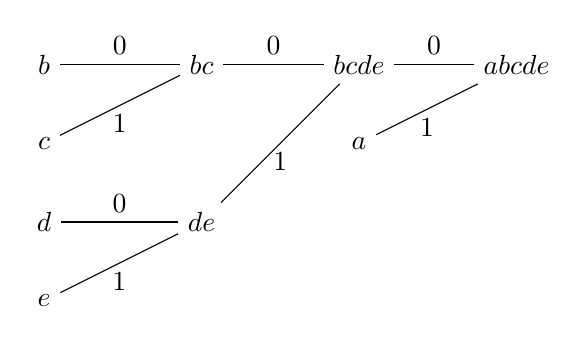
\begin{tikzpicture}[xscale=2]
    %\node (a0) at (0,4) {$a$}; %0.4
    %\node (b0) at (0,3) {$b$}; %0.2
    %\node (c0) at (0,2) {$c$}; %0.15
    \node (d0) at (1,2) {$d$}; %0.15
    \node (e0) at (1,1) {$e$}; %0.1
    
    %\node (a1) at (1,4) {$a$}; %0.4
    %\node (de1) at (1,3) {$de$}; %0.25
    \node (b1) at (1,4) {$b$}; %0.2
    \node (c1) at (1,3) {$c$}; %0.15
    
    %\node (a2) at (2,4) {$a$}; %0.4
    \node (bc2) at (2,4) {$bc$}; %0.35
    \node (de2) at (2,2) {$de$}; %0.25

    \node (bcde3) at (3,4) {$bcde$}; %0.6
    \node (a3) at (3,3) {$a$}; %0.4

    \node (abcde4) at (4,4) {$abcde$}; %1

\draw (de2) -- node[above] {$0$} ++(d0);
\draw (de2) -- node[below] {$1$} ++(e0);

\draw (bc2) -- node[above] {$0$} ++(b1);
\draw (bc2) -- node[below] {$1$} ++(c1);

\draw (bcde3) -- node[above] {$0$} ++(bc2);
\draw (bcde3) -- node[below] {$1$} ++(de2);

\draw (abcde4) -- node[above] {$0$} ++(bcde3);
\draw (abcde4) -- node[below] {$1$} ++(a3);


\end{tikzpicture}

The code is then
\begin{align*}
    C(a) &= 1\\
    C(b) &= 000\\
    C(c) &= 001\\
    C(d) &= 010\\
    C(e) &= 011
\end{align*}
The average length is then $2.2$ bits per symbol.
\end{example}


Note that there is no need for general tie-breaking rules. Indeed, different merges may yield different codes, and maybe even different code lengths, but always the same expected length. Similarly, the assignment of $0$ or $1$ does not change the code lengths.



\paragraph{Huffman codes are compact} Clearly, Huffman codes are prefix. The proof that they are compact is by induction on the number of symbols and omitted. It can be found in \cite[Section 5.8]{CT06}.


\paragraph{Non-binary Huffman codes}

Huffman codes can be extended to non-binary alphabets: If we have an alphabet of $D$ characters, we group the $D$ least likely symbols at each stage of reducing the source. When expanding the code we append each of the $D$ characters to one of the least likely symbols' codewords.

We must end up with exactly $D$ symbols in the final source, so we may need to pad the original source up to $D+k(D-1)$ by adding symbols of probability $0$.

\subsection{See further}

\paragraph{Codes and Automata} The mathematical theory of uniquely decodable codes is reviewed in \cite{BPR10}, where they are simply referred to as codes. The language generated by a prefix code can be recognised by very a simple deterministic finite automaton; in fact, the relation between codes and automata is very deep and explored throughout the book. Note that this book hardly talks about data compression!

\paragraph{Canonical Huffman codes} As we shall see in Exercise \ref{exercise:huffman_unequal_lengths}, there can be several different Huffman trees for the same source. However, there is always a so-called canonical Huffman tree (and hence code) with a special shape that can be easily computed; see \cite[3.2.2]{Say12}. We shall encounter a similar idea in Lecture \ref{sec:35}.

\paragraph{Adaptive Huffman coding} Huffman coding is based on a source $X$ with given probabilities. In general, the probability of an element is computed by its relative frequency in the message; for instance, if the message has 100 characters, 34 of them are ``e'', then the probability of ``e'' is 34\%. Computing those probabilities then requires scanning the whole document before building the tree. Adaptive Huffman coding, on the other hand, builds the Huffman tree as the document is scanned, making small updates (if any) each time a new character is scanned.

\subsection{Exercises}

\begin{exercise} \label{exercise:not_prefix}
Let $\mathcal{X} = \{x_1, \dots, x_q\}$ for $q \ge 2$. Give a binary code $C : \mathcal{X} \to \{0,1\}^*$ that is uniquely decodable but neither prefix nor suffix.
\end{exercise}

\begin{exercise} \label{exercise:prefix}
Finish the example of decoding a prefix code.
\end{exercise}

\begin{exercise} \label{exercise:decoding_prefix}
How could you make the decoding algorithm of prefix codes more efficient? Would you use that modification for decoding Huffman codes? How would you include the decision problem: given $w \in \mathcal{D}^*$, determine whether $w$ is a codeword.
\end{exercise}

\begin{exercise} \label{exercise:huffman}
Construct a binary Huffman code for $X$ with probabilities $0.5, 0.2, 0.15, 0.1, 0.05$. What is the average length, and how does it compare with the one in Example \ref{example:huffman}?
\end{exercise}

\begin{exercise} \label{exercise:huffman_unequal_lengths}
Let $X$ have probabilities $(1/3, 1/3, 1/4, 1/{12})$. Show that, depending on how you merge, the binary Huffman coding procedure may lead to different code lengths, namely $(2,2,2,2)$ or $(1,2,3,3)$. Verify that the average length remains the same, though.
\end{exercise}


\section{Statistical compression II: Arithmetic coding} 
\label{sec:02}

%\subsection{Adaptive Huffman coding}


\subsection{Arithmetic coding}


\paragraph{Limitation of Huffman coding} Consider a source with a heavily imbalanced distribution: say $a :0.99$ and $b: 0.01$. Suppose we want to encode the sequence 
\[
    m = aaaaaaaaaa
\]
(of length $10$) using Huffman coding. Then we would require $10$ bits (the length of the message). 

However, if you compute the probability of that particular $10$-character sequence, we get 
\[
    p(m) = p(a)^{10} \approx 0.904.
\]
So if we were to compute the Huffman code based on all $2^{10}$ possible sequences, $m$ would be encoded as only one bit!

The main limitation of Huffman is then apparent: the codewords are only defined for symbols, not messages. Arithmetic coding offers a way of working at the \Important{sequence level}, thereby assigning a particular tag to any sequence, without working out all the tags for all sequences of the same length.

Suppose $X = \{a_1, \dots, a_n\}$ with respective probabilities $p_1, \dots, p_n$. We want to encode the message $m = a_{i_1} \dots a_{i_k}$. The output of the arithmetic encoder will be a \Important{number} in the range $[0,1)$ that uniquely describes $m$.

\begin{example} \label{example:arithmetic}
Let $X = \{a_1, a_2, a_3\}$ with probabilities $p_1 = 0.4, p_2 = 0.5, p_3 = 0.1$. The interval $[0,1)$ is subdivided among the three symbols as 
\[
    a_1 : [0, 0.4), \quad a_2 : [0.4, 0.9), \quad a_3 : [0.9, 1). 
\]
The interval is then recursively subdivided in the same fashion, e.g. $a_1 : [0, 0.4)$ is subdivided into 
\[
    a_1a_1 : [0, 0.16), \quad a_1a_2 : [0.16, 0.36), \quad a_1a_3 : [0.36, 0.4). 
\]
The final code for $a_1a_3$ could be any number in the range $[0.36, 0.4)$. The decoding is performed by iteratively performing the splits and choosing the interval where the code belongs. For instance, say we send $c = 0.36$ (obviously, we only send $36$), then the decoder first finds out that $c \in [0, 0.4)$ hence $m_1 = a_1$; then $c \in [0.36, 0.4)$ hence $m_2 = a_2$.
\end{example}




For each symbol processed, the current interval gets smaller and requires more bits to express it, but the final output is a single number for the whole sequence, which is not simply the concatenation of the codewords for its symbols. We illustrate the encoding and decoding processes in more detail by using a slightly more complex example.



We show the compression steps for the string ``SWISS\textvisiblespace MISS''. This time, the probabilities directly arise from the character frequencies, which are computed as a preliminary step to the encoding process.\\
~\\

\begin{tabular}{l|l|l|l}
    Character $x$    & Frequency  & Probability          & Range  $[L(x), H(x) )$     \\
    \hline
    S       & 5     & 0.5    & [0.5, 1.0)         \\ 
    W       & 1     & 0.1    & [0.4, 0.5)         \\ 
    I       & 2     & 0.2    & [0.2, 0.4)         \\ 
    M       & 1     & 0.1    & [0.1, 0.2)         \\ 
    \textvisiblespace       & 1     & 0.1     & [0.0, 0.1)       
\end{tabular}
~\\
~\\

The encoding process begins by defining two variables $Low$ and $High$ and setting them to $0$ and $1$, respectively.They define an interval $[Low, High)$. As symbols are being input and processed, the values of $High$ and $Low$ are moved closer together. As the symbol $x$ is being input and processed, $Low$ and $High$ are updated according to
\begin{align*}
    High    &\gets Low + (High - Low) H(x),\\
    Low     &\gets Low + (High - Low) L(x).
\end{align*}
~\\

\begin{tabular}{l|l|l|l|l}
    $x$   & $L(x)$  & $H(x)$  & $Low$     & $High$     \\
    \hline
        &       &       & 0     & 1     \\
    S   & 0.5   & 1.0     & 0.5   & 1.0     \\
    W   & 0.4   & 0.5   & 0.70   & 0.75     \\
    I   & 0.2   & 0.4   & 0.71   & 0.72     \\
    S   & 0.5   & 1.0     & 0.715   & 0.72     \\
    S   & 0.5   & 1.0     & 0.7175   & 0.72     \\
    \textvisiblespace   & 0.0   & 0.1     & 0.7175   & 0.71775     \\
    M   & 0.1   & 0.2   & 0.717525   & 0.717550     \\
    I   & 0.2   & 0.4   & 0.717530   & 0.717535     \\
    S   & 0.5   & 1.0     & 0.7175325   & 0.717535     \\
    S   & 0.5   & 1.0     & 0.71753375   & 0.717535     
\end{tabular}
~\\

The final code is the final value of $Low$, $0.71753375$ of which only the eight digits $71753375$ need to be written.


The decoder first inputs the symbols and their range, and reconstructs the table of frequencies and probabilities. It then inputs the rest of the code. The first digit is $7$, so the number is $0.7\ldots \in [0.5, 1)$: the first symbol is then S. It carries on, updating the code number to remove the effect of the character it just input. More explicitly, after the character $x$, it performs the update
\[
    C \gets \frac{C - L(x)}{H(x) - L(x)}.
\]
The decoder carries on until $C = 0$, in which case there should be a way to make it stop (either an end-of-file symbol is part of the input, or the length of the input was given in the header of the code).\\
~\\

\begin{tabular}{l|l|l|l}
    $x$   & $L(x)$      & $H(x)$      & $C$     \\
    \hline
        &           &           & 0.71753375     \\
    S   & 0.5       & 1.0       & 0.4350675     \\
    W   & 0.4       & 0.5       & 0.350675     \\
    I   & 0.2       & 0.4      & 0.753375     \\
    S   & 0.5      & 1.0      & 0.50675     \\
    S   & 0.5      & 1.0      & 0.0135     \\
    \textvisiblespace   & 0.0      & 0.1      & 0.135     \\
    M   & 0.1      & 0.2      & 0.35     \\
    I   & 0.2      & 0.4      & 0.75     \\
    S   & 0.5      & 1.0      & 0.5     \\
    S   & 0.5      & 1.0      & 0     
\end{tabular}


\subsection{Implementation details}

\paragraph{Using integers} The encoding as described before is not practical, since it uses numbers of unlimited precision for $Low$ and $High$. The decoder process is also impractical: the number $C$ can be a very long integer.


Any practical implementation of arithmetic coding should only use integers and should not be very long. Here is an implementation that uses integers with only four digits (We only give the encoder, but the decoder can be worked out as ``doing the same in reverse,'' as we are getting used to seeing.)

The main idea is that once the leftmost digits of $Low$ and $High$ are equal, then they remain equal henceforth. So we should ``forget about'' the leftmost digit once the encoder has output it. This is done by shifting the digits. Using four digits, we first initialise $L^* = 0000$ (corresponding to $Low = 0.0000\dots = 0$) and $H^* = 9999$ (corresponding to $High = 0.9999\dots = 1$), and we proceed as follows.\\
~\\

\begin{tabular}{l|l|l|l|l|l}
    $x$   & $Low$     & $High$     & Digit & $L^*$ & $H^*$ \\
    \hline
        & 0     & 1     &       & 0000  & 9999 \\
    S   & 0.5   & 1     &       & 5000  & 9999 \\
    W   & 0.7   & 0.75  & 7     & 0000  & 4999 \\
    I    & 0.1 & 0.2 &  1     & 0000  & 9999 \\
    S    & 0.5 & 1.0 &       & 5000  & 9999 \\
    S    & 0.75 & 1.0 &       & 7500  & 9999 \\
    \textvisiblespace    & 0.75 & 0.775 &  7    & 5000  & 7499 \\
    M    & 0.525 & 0.55 &  5     & 2500  & 4999 \\
    I    & 0.3 & 0.35 & 3      & 0000  & 4999 \\
    S    & 0.25 & 0.5 &       & 2500  & 4999 \\
    S    & 0.375 & 0.5 & 3750   &   & 4999  
\end{tabular}
~\\

In this toy example, we used four digits, but in practice we should be using enough to make sure that enough information is conveyed by $H^*$ and $L^*$ at all times. Another potential issue is that of underflow, when for instance $High$ decreases too fast and loses its significant digits. Scaling is then performed to avoid this situation.

\paragraph{Using binary strings} Firstly, note that we can choose to output any number in the range $[Low, High)$, ans not necessarily $Low$ per se. A certain choice of value may have fewer digits in its binary expansion, and hence require less space than $Low$. Moreover, obviously operations should be carried out in binary instead of decimal.

It can be shown that, if one uses the number $(Low + High)/2$, then one only needs to transmit the first
\[
    l = \left\lceil \log \frac{1}{p(m)} \right\rceil + 1
\]
bits of that number, where $p(m)$ is the probability of the input sequence $m$. As we shall see in Lecture \ref{sec:35}, this is very close to optimality indeed.


\subsection{Exercises}

\begin{exercise} \label{exercise:arithmetic}
With the same source as in Example \ref{example:arithmetic}, encode the message $m = a_2a_3a_1a_1a_3$.
\end{exercise}



\begin{exercise} \label{exercise:swiss_miss}
Work out a decoder for the four-digit implementation of arithmetic coding, and decode the output of the SWISS MISS example.
\end{exercise}


% \subsection{Answers}

\section{Lempel-Ziv I: LZ77}
\label{sec:03}


\subsection{Limitations of statistical compression}

In Lectures \ref{sec:01} and \ref{sec:02} we looked at compact codes for data being emitted by a memoryless source - a random process.

This week we look at encoding a fixed file of data efficiently. Rather than having estimates for the probabilities of each symbol, we can look at the whole message and determine the frequency of each symbol. Compact codes for memoryless sources are guaranteed to be optimal on average, but we may not have an average message. If the encoding is not determined in advance (as can be done for known sources), but is message dependent, then we must transmit the code as well as the encoded message.

Recall, memoryless sources emit each symbol independently of any previous symbols. There is no 'pattern' to the data beyond the frequency of each symbol. For instance, consider the message 
\[
    abbaeadcaadccbaabaaa
\]
(20 characters). The letter frequencies are a:10/20, b:4/20, c:3/20, d:2/20, e:1/20. These agree exactly with the probabilities in Exercise \ref{exercise:huffman}. Using the Huffman code $abbaeadcaadccbaabaaa$ becomes
\[
    100001011110110010110110010010001100111
\]
(39 characters, as expected - 1.95 bits on average). 

It is not obvious that we can do better here, and in general for randomly chosen messages with these frequencies we simply can't! But what about: 
\[
    aaaaaaaaaabbbbcccdde
\]
or: 
\[
    ababababacacacadadae ?
\]
Again, Huffman coding would yield 39 characters. Clearly, those messages have more than just statistical redundancy; they also have a form of structural redundancy to which statistical methods such as Huffman coding are oblivious.





\paragraph{Source modelling}

A lot of work was done in the early days of text compression to model natural languages and to understand their redundancy. The first work is Shannon's statistical analysis of English text \cite{Sha51}, and it has been significantly refined over the years (see Cover and King \cite{CK78} for a survey of techniques). 

Using a completely different approach, Zipf \cite{Zip49} exhibited a remarkable variety of hyperbolic laws in social sciences; in particular the distribution of words in a natural language approximately satisfies the beautiful law described below. Suppose a natural language has $N$ words, sorted in non-increasing frequency ($p(1) \ge p(2) \ge \dots p(r) \dots \ge p(N)$). Then the probability of the word at the $r$-th rank is
\[
    p(r) = \frac{ \mu }{ r },
\]
with
\[
    \mu \approx \frac{ 1 }{ \log_e N + \gamma },
\]
where $\gamma = 0.577\dots$ is the Euler-Mascheroni constant. Finer models have been proposed, e.g. by Mandelbrot \cite{Man52}.

We have already looked at modelling English as a sequence of random letters with frequencies. This is called the \Define{first-order model} of English. Random text from this model (plus space) would look like:
\begin{quote}
    \texttt{ocroh hli rgwr nmielwis eu ll nbnesebya th eei alhenhttpa oobttva nah brl}
\end{quote}



We could do better by regarding English not as 26 letters, but as $26^2$ pairs of letters (\Define{digrams}), E.g. AB QU ZA QZ. If we analyse the frequencies of digrams, we can choose the next letter based upon the previous letter and the digram frequencies. E.g. Q will almost certainly be followed by U, T is most likely to be followed by H. This is called the \Define{second-order model} of English.  Random text from this model (plus space) would look like:
\begin{quote}
    \texttt{on ie antsoutinys are t inctore st be s deamy achin d ilonasive tucoowe at teasonare fuso tizin andy tobe seace ctisbe}
\end{quote}

Random text from the third-order model of English would look like:
\begin{quote}
\texttt{in no ist lat whey cratict froure birs grocid pondenome of demonstures of the reptagin is regoactiona of cre}
\end{quote}
There are finer and finer models of the English language, some based on $n$-gram frequencies, other (more accurate), based on frequencies of sequences of words. Examples of text generated from $12$-gram model (for letters) and $6$-gram model (for text) can be found in \cite[Chapter 4]{BCW90}.

One could then consider using Huffman coding (or any other statistical technique) with finer and finer models. There are two major issues with this approach.
\begin{enumerate}
    \item The alphabet of the source $X$ explodes! If we consider just the $4$-gram model (for letters), then the alphabet is of size $26^4 = 456,976$. In general, the alphabet size grows exponentially with $n$ for $n$-grams.
    
    \item The model is only appropriate for a particular sort of text. The model for English is inappropriate for German or French, let alone Greek, Russian or Chinese. So that strategy is not easily portable.
\end{enumerate}



\subsection{Lempel-Ziv}

The main idea of dictionary based compression is to construct a table (dictionary) of commonly used subsequences and refer to this to build the coded message. The main idea behind Lempel-Ziv (LZ77) is to use the message itself as a dictionary.

The LZ77 encoding algorithm works as follows. The encoding scans the message from first to last character. For implementation purposes, it uses a sliding window, of size $W$ and a look-ahead buffer of size $L$. Consider the message $m_1 \dots m_n$. When encoding at character $i$, look for the largest $l$ such that the first $l$ characters of the look-ahead buffer match $l$ consecutive characters in the sliding window, i.e. 
\[
    m_i \dots m_{i+l-1} = m_{i-d} \dots m_{i-d+l-1}
\]
where   $d \le W$ and $l \le L$. Append the coded message with $(d,l,m_{i+l})$. Resume encoding at character $i+l+1$.

The L77 decoding algorithm reads a list of triplets $(d,l,m_{i+l})$, which it interprets as the instruction: 
\begin{quote}
Print out $m_{i-d} \dots m_{i-d+l-1} m_{i+l}$ (the $l$ successive characters of $m$ starting from $d$ positions ago, and then $m_{i+l}$).
\end{quote}


\begin{example}
Encoding the sequence
\[
    ABRACADABRA
\]
using LZ77 (with say infinite $W$ and $L$) yields
\[
(0,0,A) \quad
(0,0,B) \quad
(0,0,R) \quad
(3,1,C) \quad
(2,1,D) \quad
(7,4,-)
\]
\end{example}

\begin{example}
A longer example now:
\begin{quote}
    Peter Piper picked a peck of pickled peppers;\\
    A peck of pickled peppers Peter Piper picked;\\
    If Peter Piper picked a peck of pickled peppers,\\
    Where's the peck of pickled peppers Peter Piper picked?
\end{quote}

We obtain:
\begin{align*}
&(0,0,P) (0,0,e)(0,0,t)(2,1,r)(0,0, )(6,1,i)(0,0,p)(6,3,p)(6,1,c)(0,0,k)(7,1,d)\\
&(7,1,a) (9,2,e)(9,2, )(0,0,o)(0,0,f)(17,5,l)(18,3,p)(4,1,p)(32,3,s)(0,0,;)\\
&(0,0,A)(26,24, )(71,18,;)(0,0,I)(38,2,P)(93,43,,)\\
&(0,0,W)(0,0,h)(6,2,e)(0,0,')(75,2,t)(8,2, ) (103,42,?)
\end{align*}


193 characters encoded as 34 triples.
If each triple is 3 bytes - that is 193 bytes reduced to 102 bytes.

\end{example}




\paragraph{How much space do we need?}

Each triple in the encoding includes $d \le W$, $l \le L$ and a character. For ASCII, the character takes $8$ bits. In total, we need 
\[
    \log_2 ( W + 1 ) + \log_2 (L + 1) + 8
\]
bits to encode a triple.

Typical values are $W = 2^{16} - 1 = 65535$, and $L = 2^8 - 1 = 255$, so we need $16+8+8$ bits per triple, i.e. $4$ bytes. This much can be wasteful, especially if the value of $l$ is very low ($l=0$ means that this is a new character for instance).


\subsection{Applications of LZ77}

\paragraph{LZSS} Lempel-Ziv-Storer-Szymanski (\Define{LZSS}) is a popular variant of LZ77 introduced in 1982. The main improvement is that it includes a flag to distinguish between new characters and tokens. That way, a new character does not need to be encoded as a full token, and tokens only have two fields instead of three.

\paragraph{DEFLATE} \Define{Deflate} is a lossless compression technique that combines LZSS and Huffman coding. The key idea is that Lempel-Ziv removes structural redundancy from the data, but its output still has some statistical redundancy; the latter is then removed by Huffman coding.

Deflate is everywhere: in \texttt{gzip}, in the \Important{ZIP} file format, in \Important{PNG}, etc. (Technically, ZIP allows for many different compression techniques, but Deflate is the one that's used most of the time.)

\paragraph{LZMA} The Lempel-Ziv-Markov chain algorithm (\Define{LZMA}) was developed for 7z. Its description is out of the scope of these lectures.

\subsection{See further}

\paragraph{Variants} There are many variants of LZ77, e.g. LZX, LZRW1, LZRW4. Have a look!

\paragraph{VCDIFF} \Define{File differencing} refers to any method that compresses the differences between two files (say the source and the target files). The term \Important{delta compression} is also used. VCDIFF is a method for file differencing based on LZ77. The basic idea is very simple: 
\begin{enumerate}
    \item append the target file to the source file to make one massive file

    \item use LZ77 to compress that massive file
    
    \item only save the part relating to the target file of the output of LZ77.
\end{enumerate}
The implementation is more involved; see \cite{KMMV02}. In general, delta compression is an important problem that is still the subject of ongoing research.


\subsection{Exercises}

\begin{exercise}
Decode the following string encoded with LZ77.
\begin{align*}
&(0,0,r)(0,0,i)(0,0,n)(0,0,g)(0,0, ) \\ 
& (0,0,a)(2,1,r)(7,4,o)(7,2,o)(0,0,s)(9,1,e)(3,1, )\\
& (16,2,p)(9,1,c)(0,0,k)(9,1,t)(7,1,f)(0,0,u)(0,0,l)(1,1, )\\
& (11,1,f)(15,3,s)(24,5,t)(6,1,s)(0,0,h)(11,1,o)(8,9,w)(20,1, )\\
& (11,1,l)(33,2,f)(5,4,d)(15,1,w)(0,0,n)
\end{align*}
\end{exercise}


\begin{exercise}
Watch this youtube video on the repetitiveness of pop music: \href{https://www.youtube.com/watch?v=_tjFwcmHy5M}{\textcolor{blue}{Pop Music is Stuck on Repeat}}. Can you guess which is the most repetitive song in the history of the Billboard Hot 100? 
\end{exercise}

\begin{exercise}
Write your own LZ77 encoder (in Python, Java, or any other language). Can you find famous pieces of fiction that compresses massively, or hardly at all?
\end{exercise}


\section{Lempel-Ziv II: LZ78}
\label{sec:04}


\subsection{LZ78}

\paragraph{Basic idea} The \Define{LZ78} method does not use any search buffer, look-ahead buffer, or sliding window. Instead, it simply keeps a dictionary of previously encountered strings. The dictionary starts with the empty string at position zero and its size is only limited by the memory size.

The encoder outputs \Important{two-field tokens} (instead of three-field tokens in LZ77). Each token simply corresponds to a new string in the dictionary: it is of the form
\[
    (i, x),
\]
where $i$ is the position of the longest match in the dictionary and $x$ is the final character of the string.

Nothing is ever deleted from the dictionary:
\begin{itemize}
    \item Advantage over LZ77: future strings will be compressed even if they only match strings in the distant past;
    
    \item Drawback: the dictionary can become very large!
\end{itemize}

\paragraph{Example} Once again, it is best explained via a simple example. Say we want to compress
\begin{quote}
    sir\textvisiblespace sid\textvisiblespace eastman\textvisiblespace easily%\textvisiblespace teases\textvisiblespace sea\textvisiblespace sick\textvisiblespace seals
\end{quote}

The tokens are then (in order!):\\
~\\
\begin{tabular}{l|l|l}
     Dictionary position    & String    & Token  \\
     \hline
     0                      &  $\epsilon$         &        \\
     1                        & s           &  (0, s)      \\
     2                   & i          & (0,i)       \\
     3                   &  r         & (0,r)       \\
     4                   &  \textvisiblespace         & (0,\textvisiblespace)       \\
     5                   &  si         &    (1,i)    \\
     6                   &  d         & (0,d)       \\
     7                   &  \textvisiblespace e         &  (4,e)      \\
     8                   &  a         & (0,a)       \\
     9                   &  st         &    (1,t)    \\
     10                   & m          &    (0,m)    \\
     11                   & an          &   (8,n)     \\
     12                   & \textvisiblespace ea          & (7,a)       \\
     13                   & sil          &  (5,l)      \\
     14                   & y          &    (0,y)    
\end{tabular}
~\\
And the compressed output is the list of tokens
\begin{quote}
    (0,s) (0,i) (0,r) (0,\textvisiblespace) (1,i) (0,d) (4,e) (0,a) (1,t) (0,m) (8,n) (7,a) (5,l) (0,y)
\end{quote}

Once again, the decoder sees these tokens as ``instructions.'' But following these instructions means searching in the dictionary. A useful data structure for the dictionary is a \Important{tree}, where the root is the empty string and a new string is added to the tree as a child of the string it refers to on its token. Such a tree is called a \Define{trie}.

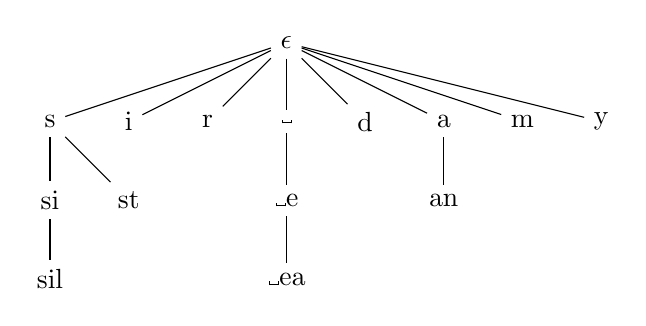
\begin{tikzpicture}
    \node (0) at (3,0) {$\epsilon$};
    
    \node (1) at (0,-1) {s};
    \node (2) at (1,-1) {i};
    \node (3) at (2,-1) {r};
    \node (4) at (3,-1) {\textvisiblespace};
    \node (5) at (0,-2) {si};
    \node (6) at (4,-1) {d};
    \node (7) at (3,-2) {\textvisiblespace e};
    \node (8) at (5,-1) {a};
    \node (9) at (1,-2) {st};
    \node (10) at (6,-1) {m};
    \node (11) at (5,-2) {an};
    \node (12) at (3,-3) {\textvisiblespace ea};
    \node (13) at (0,-3) {sil};
    \node (14) at (7,-1) {y};
    
    \draw (0) -- (1);
    \draw (0) -- (2);
    \draw (0) -- (3);
    \draw (0) -- (4);
    \draw (1) -- (5);
    \draw (0) -- (6);
    \draw (4) -- (7);
    \draw (0) -- (8);
    \draw (1) -- (9);
    \draw (0) -- (10);
    \draw (8) -- (11);
    \draw (7) -- (12);
    \draw (5) -- (13);
    \draw (0) -- (14);
    
    
\end{tikzpicture}



\subsection{LZW}


\paragraph{Basic idea} Lempel-Ziv-Welch (\Define{LZW}) is a variant of LZ78, with two main differences.
\begin{enumerate}
    \item The dictionary is \Important{initialised with all possible characters}. If we are compressing an ASCII file, then positions 0 to 255 are filled at initialisation.
    
    \item The tokens only have \Important{one field}! Since we always work with at least one character (that can always be found in the dictionary), there is no need to output the next character.
\end{enumerate}

Let us go back to our example:
\begin{quote}
    sir\textvisiblespace sid\textvisiblespace eastman\textvisiblespace easily%\textvisiblespace teases\textvisiblespace sea\textvisiblespace sick\textvisiblespace seals
\end{quote}

The dictionary is initialised with all 256 ASCII characters in positions 0 to 255, e.g. a is in position 97, b in 98, s in 115, z in 122. The first character in the string is s (in the dictionary at position 115). Since si does not appear in the dictionary, we add si to the dictionary at 256, and we continue with the character i. Again, since ir is not in the dictionary, we add ir at 257 and continue with the character r.

The dictionary (omitting positions 0 to 255) and the tokens look like this:\\
~\\
\begin{tabular}{l|l|l|l}
     Position & String & Token & What the token encodes \\
     \hline
     256 & si & 115 & s\\
     257 & ir & 105 & i\\
     258 & r\textvisiblespace & 114 & r\\
     259 & \textvisiblespace a & 32 & \textvisiblespace\\
     260 & sid & 256 & si\\
     261 & d\textvisiblespace & 100 & d\\
     262 & \textvisiblespace e & 32 & \textvisiblespace\\
     263 & ea & 101 & e\\
     264 & as & 97 & a\\
     265 & st & 115 & s\\
     266 & tm & 116 & t\\
     267 & ma & 109 & m\\
     268 & an & 97 & a\\
     269 & n\textvisiblespace & 110 & n\\
     270 & \textvisiblespace ea & 262 & \textvisiblespace e\\
     271 & asi & 264 & as\\
     272 & il & 105 & i\\
     273 & ly & 108 & l\\
        &   & 121 & y
\end{tabular}
~\\~\\
The output is then
\[
    115, 105, 114, 32, 256, 100, 32, 101, 97, 115, 116, 109, 97, 110, 262, 264, 105, 108, 121
\]

The dictionary can once again be stored as a tree, but the implementation is more complex than for LZ78. A thorough description is given in \cite[3.13.2]{Sal04}.


\subsection{Applications of LZW}

\paragraph{GIF} The ubiquitous Graphics Interchange Format (\Define{GIF}) uses a variation of LZW. It uses a dynamic, growing dictionary. It starts with the number of bits per pixel $b$: $b=2$ for monochromatic images, $b=8$ for an image with $256$ colours of shades of grey. The dictionary starts with $2^{b+1}$ entries and is doubled in size every time it fills up until it reaches $2^{12} = 4,096$ entries. At that point, the encoder may want to start a new dictionary!

GIF is not actually that good at image compression because it is unidimensional. It scans the image row after row, so it can detect similarities within a row but has trouble dealing with similarities across rows instead.

\paragraph{Limitations} One major issue of using LZW (e.g. for GIF), is that LZW is \Important{patented}. In response to that, the Portable Network Graphics format was created in the mid-90s (finalised in 96). It is based on DEFLATE (and hence LZSS) instead.

Another application of LZW was the Unix shell compression utility \texttt{compress}, that was used in the 80s. However, it was superseded by \texttt{gzip}, which typically outperforms it in terms of compression ratio.

\subsection{See further}

\paragraph{Variants} LZ78 and LZW also have a few variants, notably LZMW, LZAP and LZY. Have another look!

\paragraph{Kolmogorov complexity} The principle of Lempel-Ziv encoding is to construct a list of instructions to the decoder of the form ``Copy that string (and add that character).'' But what if we allowed any sort of instructions?

The \Define{Kolmogorov complexity} is a concept that predates Lempel-Ziv. It aims at evaluating the ``intrinsic'' complexity of a binary string. Simply put, the Kolmogorov complexity of a string $x$ w.r.t. a Turing machine $U$, denoted $K_U(x)$, is the shortest length of a program for $U$ that prints out $x$ and halts. Obviously, $K_U(x)$ is not computable. But still, we can say a lot about the Kolmogorov complexity of a random string: it's about the length of the string. Therefore, almost any string is incompressible! The study of Kolmogorov complexity and associated concepts (e.g. Solomonoff's universal probability or Chaitin's Omega number) is very intriguing but outside the scope of this course.



 \subsection{Exercises}

\begin{exercise}
Encode the string
\begin{quote}
    sir\textvisiblespace sid\textvisiblespace eastman\textvisiblespace easily\textvisiblespace teases\textvisiblespace sea\textvisiblespace sick\textvisiblespace seals
\end{quote}
with LZ78: give the dictionary table, the trie, and the output.

Encode the same string with LZW.
\end{exercise}


\begin{exercise}
Select a few (small) images, and compare the file sizes for those when saved as .bmp, .gif and .png.
\end{exercise}





\section{Context-based compression}
\label{sec:05}



\subsection{Context}

\paragraph{Context-based compression} Statistical compression (mainly for text, but not only) can be based on two properties. The first property is the frequency of symbols: the model assigns probabilities to the symbol according to their frequency in the document. 

The second one is the \Important{context}. In practice, the context a symbol consists of the $N$ symbols preceding it (note that we cannot use symbols succeeding it, as the decoder typically does not know them yet!). Context-based compression then uses the context of a symbol to \Important{predict} it (i.e. to assign it a probability). 

For instance, let's use a context of only one character. The letter h occurs in typical English text only about 5\% of the time. However, if the current symbol is t, then there is a much higher probability (around 30\%) that the next symbol will be h, since the digram th is very common in English. Note that the prediction is about assigning probabilities, not trying to figure out the next symbol exactly (which is impossible).

\paragraph{Static v Adaptive contexts} A static context-based modeler always uses the same probabilities, which are stored in some large table. Those probabilities are usually obtained by crawling through many documents (say typical English texts). There are issues with that approach, notably the fact that this might assign zero probabilities to some strings.

An adaptive context-based modeler also maintains tables of probabilities of all the possible digrams (or trigrams, or even longer $n$-grams). But this time the tables are updated all the time as more data are input, which adapts the probabilities to the particular data being compressed. \Important{Adaptive context-based compression} might be slower, but typically results in better compression.



\paragraph{Context length} One may think at first that the larger the number $N$ of symbols in the context, the better the compression. However, this might not be the case:
\begin{enumerate}
    \item A large $N$ requires to write the first $N$ symbols in plain text, which might hurt the overall compression.
    
    \item If $N$ is too large, then there are simply too many contexts, which makes storing, reading off, and writing on the table of probabilities infeasible.
    
    \item A very long context contains information about the nature of old data. It is not uncommon to have files where different parts have different symbol distributions.
\end{enumerate}
Therefore, in practice relatively small contexts are used in practice (for text compression, traditional methods use no more than 10 characters).


\subsection{PPM}

\paragraph{Basic idea} Prediction by Partial Matching (\Define{PPM}) is based on an encoder that keeps a statistical model of the text. It starts with an order-$N$ context. It searches its data structure for an occurrence of the current context $C$ followed by the next symbol $S$. If it finds no such occurrence, if decreases the order of the context to $N-1$ and tries again (the new context $C'$ is the final $N-1$ characters of $C$). It keeps \Important{shortening the context} until it is successful. 

The encoder reads the next symbol $S$ from the input stream, looks at the current order-$N$ context $C$ (the last $N$ symbols read), and based on the previous input data, computes the probability $P$ that $S$ will appear following $C$. The encoder then calls an adaptive arithmetic encoder to encode $S$ with probability $P$. If the probability $P$ is zero, the PPM encoder tries with a smaller context; it reduces the context until $P \ne 0$. What if the symbol $S$ has not been seen yet (and hence, even with order-$0$ context, we still have $P = 0$)? Then the PPM encoder enters \Define{order-$(-1)$ context}, where the probability of $S$ is simply $1/$(size of alphabet).

\begin{example} \label{example:ppm_contexts}
Let us look at the contexts and frequency counts for the following string with $11$ symbols:
\begin{quote}
    xyzzxyxyzzx
\end{quote}

\begin{tabular}{r l | r l | r l | r l | r l}
    Order 4 & & Order 3 & & Order 2 & & Order 1 & & Order 0 &   \\
    \hline
    xyzz $\to$ x & 2 & xyz $\to$ z & 2 & xy $\to$ z & 2 & x $\to$ y & 3 & x & 4\\
    yzzx $\to$ y & 1 & yzz $\to$ x & 2 & xy $\to$ x & 1 & y $\to$ z & 2 & y & 3\\
    zzxy $\to$ x & 1 & zzx $\to$ y & 1 & yz $\to$ z & 2 & y $\to$ x & 1 & z & 4\\
    zxyx $\to$ y & 1 & zxy $\to$ x & 1 & zz $\to$ x & 2 & z $\to$ z & 2 &  & \\
    xyxy $\to$ z & 1 & xyx $\to$ y & 1 & zx $\to$ y & 1 & z $\to$ x & 2 &  & \\
    yxyz $\to$ z & 1 & yxy $\to$ z & 1 & yx $\to$ y & 1 & & &  & 
\end{tabular}
\end{example}


Now, how does the encoder tell the decoder which order context it is currently using (and hence what the decoder should be using too)? The answer is to have a dedicated \Important{escape symbol}, which we'll denote esc, which should be output whenever the context size is decreased. Since this is a new character, we should also assign a probability for the escape symbol for every encountered context. There are various ways (heuristics) of assigning such probabilities. Here, we will use the so-called Method A, where the escape symbol is assigned a frequency of 1.


We are now in position to give a more explicit example. Encoding a full sequence is actually quite tedious to explain so we'll only encode a few characters. We use contexts of order at most 2. Let us consider
\begin{quote}
    this\textvisiblespace is\textvisiblespace the\textvisiblespace tithe
\end{quote}
The first few symbols are not very interesting, so let us skip forward. Let's assume we have already encoded ``this\textvisiblespace is'' and we wish to encode the next character \textvisiblespace. 

We assume the word length for arithmetic coding is six bits (we used four decimal digits in our example in Lecture \ref{sec:02}). For the sake of simplicity, we have $Low = 0$ and hence $L^* = 000000$ and $High = 1$ hence $H^* = 111111$. (As we shall see, the low and high values may vary over time.)

Here is what the table of contexts looks like\\
~\\
\begin{tabular}{lr | lr | lr}
    Order 2 &           & Order 1 & & Order 0   \\
    \hline
    th $\to$ i      & 1 & t $\to$ h & 1 & t & 1\\
    th $\to$ esc    & 1 & t $\to$ esc & 1 & h & 1 \\
    hi $\to$ s      & 1 & h $\to$ i & 1 & i & 2\\
    hi $\to$ esc    & 1 & h $\to$ esc & 1 & s & 2 \\
    \Important{is $\to$ \textvisiblespace}      & \Important{1} & i $\to$ s & 2 & \textvisiblespace & 1\\
    \Important{is $\to$ esc}    & \Important{1} & i $\to$ esc & 1 & esc & 1 \\
    s\textvisiblespace $\to$ i      & 1 & \textvisiblespace $\to$ i & 1 \\
    s\textvisiblespace $\to$ esc    & 1 & \textvisiblespace $\to$ esc & 1 \\ 
    \textvisiblespace i $\to$ s      & 1 & s $\to$ \textvisiblespace & 1 \\
    \textvisiblespace i $\to$ esc    & 1 & s $\to$ esc & 1  
\end{tabular}
~\\
~\\
The  second-order context is ``\Important{is}''. We use characters in the order of the table: the first row gives the first interval and so on. In this context, the probability of the space sign ``\textvisiblespace'' and the probability of the escape symbol esc are both equal to 1/2, and
\[
    L(\text{\textvisiblespace}) = 0, H(\text{\textvisiblespace}) = 1/2 = L(esc), H(esc) = 1. 
\]    
    The update equations for the new $Low$ and $High$ are
\begin{align*}
    Low &\gets Low + (High - Low) L(x) = 0,\\
    L^* &\gets 000000,\\
    High & \gets Low + (High - Low) H(x) = 1/2,\\
    H^* &\gets 011111.
\end{align*}
Since the first (most significant) bit of $L^*$ and $H^*$ coincide, we shift that bit out and shift $0$ into $L^*$ and shift $1$ into $H^*$. So we obtain:
\begin{enumerate}
    \item Encoded sequence for ``\textvisiblespace'': $0$,
    
    \item Lower bound $L^* = 000000$,
    
    \item Higher bound $H^* = 111111$.
\end{enumerate}

The table of contexts now becomes:\\
~\\
\begin{tabular}{lr | lr | lr}
    Order 2 &           & Order 1 & & Order 0   \\
    \hline
    th $\to$ i      & 1 & t $\to$ h & 1 & \Structure{t} & \Structure{1}\\
    th $\to$ esc    & 1 & t $\to$ esc & 1 & h & 1 \\
    hi $\to$ s      & 1 & h $\to$ i & 1 & i & 2\\
    hi $\to$ esc    & 1 & h $\to$ esc & 1 & s & 2 \\
    is $\to$ \textvisiblespace      & 2 & i $\to$ s & 2 & \textvisiblespace & 2\\
    is $\to$ esc    & 1 & i $\to$ esc & 1 & esc & 1 \\
    \Structure{s\textvisiblespace $\to$ i}      & \Structure{1} & \Structure{\textvisiblespace $\to$ i} & \Structure{1} \\
    \Structure{s\textvisiblespace $\to$ esc}    & \Structure{1} & \Structure{\textvisiblespace $\to$ esc} & \Structure{1} \\ 
    \textvisiblespace i $\to$ s      & 1 & s $\to$ \textvisiblespace & 2 \\
    \textvisiblespace i $\to$ esc    & 1 & s $\to$ esc & 1  
\end{tabular}
~\\
~\\
The next symbol is ``t''. The second-order context is ``\Structure{s\textvisiblespace }''. Since ``t'' has zero frequency in this context, we need to encode the escape symbol. By a similar argument as above, we obtain
\begin{enumerate}
    \item Encoded escape symbol sequence: $1$,
    
    \item Lower bound $L^* = 000000$,
    
    \item Higher bound $H^* = 111111$.
\end{enumerate}
We need to look at the first-order context, which is ``\Structure{\textvisiblespace}''. Again, ``t'' does not appear with this context, so we encode another escape symbol. We obtain
\begin{enumerate}
    \item Encoded escape symbol sequence: $1$,
    
    \item Lower bound $L^* = 000000$,
    
    \item Higher bound $H^* = 111111$.
\end{enumerate}
We need to look at the zero-th order context. This time, ``t'' has already appeared, and is assigned the interval $[0, 1/9 )$. We then have 
\begin{align*}
    Low &\gets Low + (High - Low) L(x) = 0,\\
    L^* &\gets 000000,\\
    High & \gets Low + (High - Low) H(x) = 1/9,\\
    H^* &\gets 000111.
\end{align*}
Since the three leftmost bits are equal, we shift them out. We finally obtain
\begin{enumerate}
    \item Encoded sequence: for ``t'': $000$,
    
    \item Lower bound $L^* = 000000$,
    
    \item Higher bound $H^* = 111111$.
\end{enumerate}
So, to encode ``\textvisiblespace t'', we have transmitted $011000$.

Note that there would be a slight difference in practice: to keep everything integral, we would use $High = 63$, $Low = 0$ and perform an update of the form
\begin{align*}
    Low &\gets Low + \left\lfloor (High - Low + 1) \frac{ 1 }{ 9 }  \right\rfloor  = 0 = 000000\\
    High & \gets High + \left\lfloor (High - Low + 1) \frac{ 1 }{ 9 }  \right\rfloor - 1  = 6 = 000110
\end{align*}
Then we would have: Higher bound $H^* = 110111$.



\paragraph{Methods B and C} Two other main ways of assigning frequencies to the escape symbols aim to make the escape symbol more probable, which typically reduces the size of the resulting sequence for that symbol. The main idea is that if a context is followed by many different characters, then you are likely to encounter yet another character following that same context. For instance, think of the context ``s'' in English, which can be followed by virtually any other letter. \Important{Methods B and C} give the escape symbol a count equal to the number of symbols following the context; Method B then subtracts the count of every other symbol by one, while Method C does not amend those.


\subsection{See further}

\paragraph{RAR} The main application of PPM is in the Roshal Archive (\Define{RAR}) file format. 


\paragraph{Context mixing} In \Define{context mixing}, the next-symbol predictions of two or more statistical models are combined to yield a prediction that is often more accurate than any of the individual predictions. The \Important{PAQ} series of data compression programs use context mixing; they are the cutting edge in lossless compression in terms of compression ratio (at the expense of speed and memory usage) \cite{KF11}. 

Note that the problem of mixing different contexts is a very challenging issue in machine learning; that could be a very interesting topic for a project...


\paragraph{BWT} The Burrows-Wheeler transform (\Define{BWT}) is a very clever way of converting a list of symbols into one that is much more structured. You only need a little more information to make sure that the transform does not lose any information. By structured, we mean that it is ``almost sorted.'' After the transform, one can use very simple techniques to efficiently encode the structured list. Unfortunately, BWT-based compression requires to scan and to manipulate the whole message, which is an important drawback compared to the adaptive PPM.


\subsection{Exercises}


\begin{exercise} \label{exercise:ppm_contexts}
Update the table in Example \ref{example:ppm_contexts} if the following character is x.
\end{exercise}

\begin{exercise}
Finish the encoding of the sequence ``this\textvisiblespace is\textvisiblespace the\textvisiblespace tithe''. To update $High$ and $Low$, you may use our simple technique based on rational numbers, or use the version with integers instead.
\end{exercise}

















\section{Transform coding I: Mathematical background}
\label{sec:06}



\subsection{Fourier series and Fourier transform}

\paragraph{Fourier series}
The representation of periodic functions in terms of a series of sines and cosines was first used by Fourier in 1812. This idea has spread like wildfire across mathematics and its applications and is used in a ridiculous range of areas under different guises.

In this section, we want to give an introduction to Fourier series. We shall be rather informal: we will not prove many of the claimed results, and we will not worry about the precise assumptions we make.

Let $f$ be a periodic function of period $T$, i.e.
\[
    f(t) = f(t + nT) \quad \forall t \in \R, n \in \Z.
\]
Then we can write $f(t)$ as
\[
    f(t) = \sum_{k=-\infty}^\infty c_k e^{\i k \omega t},
\]
where $\i = \sqrt{-1}$ and
\[
    \omega = \frac{2 \pi}{ T }.
\]
Equivalently, we have
\[
    f(t) = a_0 + \sum_{k=1}^\infty a_k \cos ( k \omega t ) + \sum_{k=1}^\infty b_k \sin ( k \omega t ).
\]
In other words, the periodic functions of period $T$ form a vector space, and $\{ e^{\i n \omega t} \}$ forms a basis. In fact, this basis is orthonormal w.r.t. the inner product
\[
    \langle f(t), g(t) \rangle = \frac{1}{T} \int_0^T f(t) g^*(t) \ dt, 
\]
where $g^*(t)$ denotes the complex conjugate of $g$. The coefficients can then be obtained as follows:
\begin{equation} \label{eq:fourier}
    c_k = \langle f(t), e^{\i k \omega t} \rangle = \frac{1}{T} \int_0^T f(t) e^{-\i k \omega t} dt. 
\end{equation}

The intuition behind this representation is as follows. Suppose we have a periodic signal $f$. Then its $c_k$ Fourier coefficients decompose the signal into basic fluctuating signals; each $e^{\i k \omega t}$ fluctuates at a frequency of $k \omega/(2 \pi)$. As such, these coefficients give us a measure of the different amounts of fluctuation in the signal.

\paragraph{Discrete Fourier transform}
We want to handle signals that are not periodic, but instead limited in time. Suppose we have a signal $f(t)$ that is limited in time (say from $t=0$ to $t = t_1$). Then we can extend it to a periodic signal by doing
\[
    f_P(t) = \sum_{n \in \Z} f(t - nT),
\]
where $T > t_1$. This is the so-called periodic extension of $f$.

Moreover, we are dealing with discrete signals: instead of $f(t)$, we are considering $\{f_0, f_1, \dots, f_{N-1} \}$. We can discretise Equation \eqref{eq:fourier} as follows:
\[
    F_k = \frac{1}{\sqrt{N}} \sum_{n=0}^{N-1}  f_n e^{-\i \frac{2 \pi k n }{N}} \quad k = 0, 1, \dots, N-1.
\]
The coefficients $F_k$ are called the discrete Fourier transform (\Define{DFT}) of $f$. We can recover the signal from its DFT by
\[
    f_n = \frac{1}{\sqrt{N}} \sum_{k=0}^{N-1} F_k e^{\i \frac{2 \pi k n }{N}} \quad n = 0, 1, \dots, N-1.
\]

\paragraph{Matrix representation of DFT}
Let $f = (f_0, f_1, \dots, f_{N-1})$ and let $F = (F_0, \dots, F_{n-1})$ be its DFT. Then we have
\[
    F = {\bf A} f,
\]
where ${\bf A}$ is an $N \times N$ matrix with coefficients 
\[
    a_{i,j} = \frac{1}{\sqrt{N}} e^{- \i \frac{2\pi}{N} ij}.
\]
For example, with $N = 4$ we obtain
\[
    {\bf A} = \frac{1}{\sqrt{4}} \begin{pmatrix}
    1 & 1 & 1 & 1\\
    1 & -\i & -1 & \i\\
    1 & -1 & 1 & -1\\
    1 & \i & -1 & -\i
    \end{pmatrix}
\]

\paragraph{Unitary and orthogonal transforms}
The matrix ${\bf A}$ from the DFT is \Define{unitary}: it satisfies
\[
    {\bf A}^\dagger = {\bf A}^{-1},
\]
where ${\bf A}^\dagger$ is its conjugate transpose: $a^\dagger_{i,j} = a_{j,i}^*$. It is easily shown that the following are equivalent for a matrix ${\bf U}$:
\begin{enumerate}
    \item ${\bf U}$ is unitary;
    
    \item ${\bf U}$ preserves the inner product, i.e.
    \[
        \langle x,y \rangle = \langle {\bf U} x, {\bf U}y \rangle;
    \]

    \item ${\bf U}$ preserves the norm, i.e.
    \[
         \| x \|^2 = \sum_{i=0}^{N-1} |x_i|^2 = \langle x,x \rangle = \langle {\bf U} x, {\bf U}x \rangle = \sum_{i=0}^{N-1} |({\bf U}x)_i|^2 = \| {\bf U} x \|^2.
    \]
\end{enumerate}

We will not actually use the DFT and instead we will restrict ourselves to real matrices. A real unitary matrix is called \Define{orthogonal}. So an orthogonal matrix is a real matrix ${\bf A}$ such that 
\[
    {\bf A}^{-1} = {\bf A}^\top.
\]



\subsection{Two-dimensional transforms}

\paragraph{Two-dimensional data}
In general, in one dimension, we could apply any orthogonal transform as such:
\[
    \theta = {\bf A}x, \quad x = {\bf A}^\top \theta.
\]
We will use transforms for two-dimensional data (small blocks of pixels). How are we going to apply a one-dimensional transform to two-dimensional data? The answer is actually easy: we apply the transform column-wise and row-wise.

\paragraph{Matrix form} More succinctly, let ${\bf X}$ be an $N \times N$ matrix with entries $\{x_{i,j} : i,j = 0, \dots, N-1\}$. We then perform
\[
    \Theta = {\bf A} {\bf X} {\bf A}^\top.
\]
($\Theta$ is another $N \times N$ matrix.) Multiplying on the left by ${\bf A}$ performs the transform column-wise, while multiplying on the right by ${\bf A}^\top$ performs the transform row-wise. By associativity, 
\[
    \Theta = ({\bf A} {\bf X}) {\bf A}^\top = {\bf A} ( {\bf X} {\bf A}^\top ),
\]
and hence the order does not matter!

Note that the inverse is straightforward:
\[
    {\bf X} = {\bf A}^\top \Theta {\bf A}.
\]

\paragraph{Basis matrices}
Let ${\bf X}$ be an $N \times N$ matrix. For all $i,j \in \{0, \dots, N-1\}$, let ${\bf E}_{i,j}$ be the matrix with a single $1$ in position $(i,j)$ and $0$ everywhere else. Then those matrices form a basis for the vector space of all $N \times N$ matrices, and we have the decomposition
\[
    {\bf X} = \sum_{i=0}^{N-1} \sum_{j=0}^{N-1} x_{i,j} {\bf E}_{i,j}.
\]
(Trivial, isn't it?)

Any two-dimensional orthogonal transform also yields a similar decomposition. We still denote $\Theta = {\bf A} {\bf X} {\bf A}^\top$, and we denote the entries of $\Theta$ as $\theta_{i,j}$. We then have
\begin{align*}
    {\bf X} &= {\bf A}^\top \Theta {\bf A}\\
            &= {\bf A}^\top \left( \sum_{i,j} \theta_{i,j} {\bf E}_{i,j} \right) {\bf A}\\
            &= \sum_{i,j} \theta_{i,j} {\bf A}_{i,j},
\end{align*}
where the matrices ${\bf A}_{i,j} := {\bf A}^\top {\bf E}_{i,j} {\bf A}$ are the \Define{basis matrices} of the transform. More concretely, denote the $k$-th row of ${\bf A}$ as $a_k$, then
\[
    {\bf A}_{i,j} = a_i^\top a_j.
\]

For instance, let 
\[
    {\bf A} =  \frac{1}{ \sqrt{2} }
    \begin{pmatrix}
    1 & 1\\
    1 & -1
    \end{pmatrix}.
\]
Then the four basis matrices are given by
\begin{alignat*}{3}
    {\bf A}_{0,0} &= \frac{1}{2}
    \begin{pmatrix}
    1 & 1\\
    1 & 1
    \end{pmatrix} & 
    \qquad & &
    {\bf A}_{0,1} &= \frac{1}{2}
    \begin{pmatrix}
    1 & -1\\
    1 & -1
    \end{pmatrix} \\
    {\bf A}_{1,0} &= \frac{1}{2}
    \begin{pmatrix}
    1 & 1\\
    -1 & -1
    \end{pmatrix} & 
    \qquad & &
    {\bf A}_{1,1} &= \frac{1}{2}
    \begin{pmatrix}
    1 & -1\\
    -1 & 1
    \end{pmatrix}.
\end{alignat*}




\subsection{Modus operandi of transform coding}


\paragraph{Norm and energy} 
The square of the norm of a vector can be viewed as its \Important{energy}. Orthogonal transforms preserve the energy (as they are unitary matrices). The efficacy of a transform depends on how much energy compaction is provided by the transform. Intuitively, the transform helps to accumulate the energy on a few symbols; those symbols should be kept, while the other ones can be discarded at little loss. 

One measure of the energy compaction offered by a transform is the \Define{transform coding gain}, defined as follows (for simplicity, we define it for one-dimensional data). Let $\sigma_i^2$ be the variance of the transformed coefficient $\theta_i$ for $i=0, \dots, N-1$, then the transform coding gain is the ration of the arithmetic mean of variances over their geometric mean:
\[
    G_{\mathrm{TC}} := \frac{ \frac{1}{N} \sum_{i=0}^{N-1} \sigma_i^2 }{ \left(\sum_{i=0}^{N-1} \sigma_i^2 \right)^{\frac{1}{N}} }.
\]
(The derivation of this gain is out of the scope of this course.)


\paragraph{Three steps of transform coding}
Transform coding consists of three steps.
\begin{description}
\item[Step 1: Transform] First, the data is split into blocks of size $N$. Each block is mapped into a transform sequence using a reversible transform (usually orthogonal).

\item[Step 2: Quantization] Secondly, the transformed sequence is quantized. The quantization strategy depends on three main factors:
\begin{enumerate}
    \item the desired average bit rate
    
    \item the statistics of the various elements of the transformed sequence
    
    \item the effect of distortion in the transformed coefficients on the reconstructed sequence.
\end{enumerate}
Quantization is an important problem with some nice maths behind it, but we will skip the details here.

\item[Step 3: Encoding] Thirdly, the quantized value is encoded using some binary encoding technique, e.g. Huffman or arithmetic coding.
\end{description}









\subsection{See further}

\paragraph{FFT} The Fast Fourier Transform (\Define{FFT}) is, as its name suggests, a very efficient way of computing the DFT via divide and conquer. It was due to Cooley and Tuckey in 1965\dots even though Gauss had already discovered it in 1805!


\paragraph{Karhunen-Lo\`eve transform}
The \Define{KL} transform is the one that maximises the transform coding gain. However, it is based on the actual data and is impractical for our purposes.













\subsection{Exercises}

\begin{exercise}
Walsh-Hadamard transform. For all $N$ a power of $2$, the discrete Walsh-Hadamard transform (\Define{DWHT}) is defined as follows. For $N = 1$, let ${\bf H}_1 = (1)$. For $N \ge 1$, let
\[
    {\bf H}_{2N} = C \begin{pmatrix}
    {\bf H}_N & {\bf H}_N\\
    {\bf H}_N & - {\bf H}_N
    \end{pmatrix}.
\]
(This transform comes under different names; to make matters worse, those matrices are sometimes called Sylvester matrices.)
\begin{enumerate}
    \item Verify that the Discrete Walsh-Hadamard Transform is indeed orthogonal for the right choice of constant $C$. 

    \item Give ${\bf H}_2$, ${\bf H}_4$ and ${\bf H}_8$.
    
    \item Give all sixteen basis matrices for $N = 4$.
    
    \item Find a closed form formula for the $(i,j)$ entry of ${\bf H}_N$.
\end{enumerate}
\end{exercise}


\begin{exercise}
Give the sixteen basis matrices for the DFT with $N = 4$.
\end{exercise}

\begin{exercise}
Consider the data
\[
    {\bf X} = \begin{pmatrix}
    4 & 3 & 2 & 1\\
    3 & 2 & 1 & 1\\
    2 & 1 & 1 & 0\\
    1 & 1 & 0 & 1
    \end{pmatrix}.
\]
\begin{enumerate}
    \item Compute its two-dimensional DFT.
    
    \item Compute its two-dimensional DWHT.
\end{enumerate}
\end{exercise}










\section{Transform coding II: JPEG}
\label{sec:07}


\subsection{Operations before transform coding}

\paragraph{Color space transformation}
First, the image should be converted from RGB into a different color space called \Important{$Y'C_BC_R$} (a.k.a. YCbCr). It has three components $Y'$, $C_B$ and $C_R$: the $Y'$ component represents the \Important{brightness} of a pixel, and the $C_B$ and $C_R$ components represent the \Important{chrominance} (split into blue and red components). 

Mathematically, let $R, B, G$ be the red, green and blue signals, which all take a value between $0$ and $1$. Then
\begin{align*}
    Y' &= K_R R + K_G G + K_B B,\\
    C_B &= \frac {1}{2} \frac {B-Y'}{1-K_B},\\
    C_R &=\frac {1}{2} \frac {R-Y'}{1-K_R},
\end{align*}
where $K_R$, $K_G$, and $K_B$ are constants that satisfy $K_R + K_G +K_B = 1$. For instance, 
\begin{align*}
    K_R &= 0.299,\\
    K_G &= 0.587,\\
    K_B &=0.114.
\end{align*}

The YCbCr colour space conversion allows greater compression without a significant effect on perceptual image quality (or greater perceptual image quality for the same compression). The compression is more efficient because the brightness information, which is more important to the eventual perceptual quality of the image, is confined to a single channel. This more closely corresponds to the perception of color in the human visual system.


\includegraphics[height=10cm]{DataCompression/YCbCr.jpg}


\paragraph{Downsampling}
Humans can see considerably more fine detail in the brightness of an image (the Y' component) than in the hue and color saturation of an image (the Cb and Cr components). As such, the next step is \Important{chroma downsampling}, which reduces the spatial resolution of the Cb and Cr components. 



\paragraph{Block splitting} 
JPEG splits an image into $8 \times 8$ blocks of pixels and applies transform coding to each block. We will focus on one channel and see the data as an $8 \times 8$ matrix of integers ${\bf X}$. We will use a running example with
\[
    {\bf X} = \begin{pmatrix}
    124 & 125 & 122 & 120 & 122 & 119 & 117 & 118\\
    121 & 121 & 120 & 119 & 119 & 120 & 120 & 118\\
    126 & 124 & 123 & 122 & 121 & 121 & 120 & 120\\
    124 & 124 & 125 & 125 & 126 & 125 & 124 & 124\\
    127 & 127 & 128 & 129 & 130 & 128 & 127 & 125\\
    143 & 142 & 143 & 142 & 140 & 139 & 139 & 139\\
    150 & 148 & 152 & 152 & 152 & 152 & 150 & 151\\
    156 & 159 & 158 & 155 & 158 & 158 & 157 & 156
    \end{pmatrix}.
\]


\subsection{Step 1: Transform}

\paragraph{DCT}
The discrete cosine transform (\Define{DCT}) is similar to the DFT, but only takes the cosines into consideration. More precisely, the transform matrix is ${\bf C}$, where
\[
    c_{i,j} = C_i \sqrt{ \frac{1}{N} } \cos \left( \frac{(2j+1)i \pi}{2 N} \right),
\]
where $C_0 = 1$ and $C_i = 2$ for all $i \in \{1, \dots, N-1\}$. The basis matrices for the DCT ($N=8$) are given below.

\begin{center}
\includegraphics[width=10cm]{DataCompression/DCT-8x8.png}
\end{center}

Technically, JPEG does not apply the DCT to ${\bf X}$ directly. Instead, it subtracts $128$ to each value (so that for instance, the top left value is now -4) before applying the DCT. Following our running example, we obtain
\[
    \Theta = \begin{pmatrix}
    39.88 & 6.56 & -2.24 & 1.22 & -0.37 & -1.08 & 0.79 & 1.13\\
    -102.43 & 4.56 & 2.26 & 1.12 & 0.35 & -0.63 & -1.05 & -0.48\\
    37.77 & 1.31 & 1.77 & 0.25 & -1.50 & -2.21 & -0.10 & 0.23\\
    -5.67 & 2.24 & -1.32 & -0.81 & 1.41 & 0.22 & -0.13 & 0.17\\
    -3.37 & -0.74 & -1.75 & 0.77 & -0.62 & -2.65 & -1.30 & 0.76\\
    5.98 & -0.13 & -0.45 & -0.77 & 1.99 & -0.26 & 1.46 & 0.00\\
    3.97 & 5.52 & 2.39 & -0.55 & -0.051 & -0.84 & -0.52 & -0.13\\
    -3.43 & 0.51 & -1.07 & 0.87 & 0.96 & 0.09 & 0.33 & 0.01
    \end{pmatrix}.
\]



\paragraph{DCT over DFT} Why use the DCT instead of the DFT? Let's use the one-dimensional case to explain this. The DFT has a major problem: it ``presumes'' that the signal $(f_0, \dots, f_{N-1})$ has period $N$, since it uses a basis a functions that are periodic of period $N$. But there could be a large \Important{discontinuity} in our signal: $f_0$ may differ from $f_{N-1}$. The DFT needs accounts for that discontinuity by adding a term of high frequency and in turn modifying all the lower frequency terms: that can ruin everything. On the other hand, the DCT ``presumes'' that the signal has period $2N$ by effectively working on a new signal $(f_0, \dots, f_{N-1}, f_{N-1}, f_{N-2}, \dots, f_0)$. That signal does not have such discontinuity anymore. See below for an example; note that there are four main kinds of DCT and that JPEG uses DCT-II.

\begin{center}
\includegraphics[width=10cm]{DataCompression/DCT.png}
\end{center}




\subsection{Step 2: Quantization}

\paragraph{Zigzag scan}

The basis matrices of the DCT represent different fluctuations of frequency increasing with both $i$ and $j$. In particular, the $\theta_{0,0}$ coefficient is referred to as the \Define{DC} coefficient as it corresponds to zero frequency and is proportional to the average value of $x_{i,j}$. The other coefficients are referred to as the \Define{AC} coefficients.  The coefficients are sorted according to a \Important{zigzag scan}, displayed below.

\begin{center}
\includegraphics[width=6cm]{DataCompression/JPEG_ZigZag.png}
\end{center}


\paragraph{Quantization}
The JPEG algorithm uses so-called ``uniform midtread quantization.'' The quantization steps are organized in a quantization table; an example is given in the following matrix.
\[
    {\bf Q} = \begin{pmatrix}
    16 & 11 & 10 & 16 & 24 & 40 & 51 & 61\\
    12 & 12 & 14 & 19 & 26 & 58 & 60 & 55\\
    14 & 13 & 16 & 24 & 40 & 57 & 69 & 56\\
    14 & 17 & 22 & 29 & 51 & 87 & 80 & 62\\
    18 & 22 & 37 & 56 & 68 & 109 & 103 & 77\\
    24 & 35 & 55 & 64 & 81 & 104 & 113 & 92\\
    49 & 64 & 78 & 87 & 103 & 121 & 120 & 101\\
    72 & 92 & 95 & 98 & 112 & 100 & 103 & 99
    \end{pmatrix}
\]
These values are actually determined by a quality coefficient specified by the user.

The quantized value of $\theta_{i,j}$ is
\[
    l_{i.j} = \left\lfloor \frac{ \theta_{i,j} }{ Q_{i,j} } \right\rceil,
\]
where $\lfloor x \rceil$ denotes the integer nearest to $x$: $\lfloor x \rceil = \lfloor x + 0.5 \rfloor$. 


We can see that the step size increases as we move from the DC coefficient to higher frequency coefficients. Therefore, more quantization error will be introduced at higher-frequency levels. This is because quantization errors in the DC and lower AC coefficients are more easily detectable by the human visual system than quantization errors in the higher AC frequencies.

Following our example, we obtain the following quantized coefficients
\[
    {\bf L} = \begin{pmatrix}
    2 & 1 & 0 & 0 & 0 & 0 & 0 & 0\\
    -9 & 0 & 0 & 0 & 0 & 0 & 0 & 0\\
    3 & 0 & 0 & 0 & 0 & 0 & 0 & 0\\
    0 & 0 & 0 & 0 & 0 & 0 & 0 & 0\\
    0 & 0 & 0 & 0 & 0 & 0 & 0 & 0\\
    0 & 0 & 0 & 0 & 0 & 0 & 0 & 0\\
    0 & 0 & 0 & 0 & 0 & 0 & 0 & 0\\
    0 & 0 & 0 & 0 & 0 & 0 & 0 & 0
    \end{pmatrix}
\]

All coefficients with magnitude less than half the corresponding step size will be set to zero. Because the step sizes at the end of the zigzag scan are larger, we typically see a \Important{long run of zeroes} toward the end of the scan. The entire run of zeroes at the end of the scan can be code by an end of block (\Important{EOB}) code after the last nonzero label.


Reconstruction at the decoder's end is straightforward: the reconstructed value $\hat{\theta}_{i,j}$ is given by 
\[
    \hat{\theta}_{i,j} = l_{i,j} Q_{i,j}.
\]
In our example, we obtain
\[
    \hat{\Theta} = \begin{pmatrix}
    32 & 11 & 0 & 0 & 0 & 0 & 0 & 0\\
    -108 & 0 & 0 & 0 & 0 & 0 & 0 & 0\\
    42 & 0 & 0 & 0 & 0 & 0 & 0 & 0\\
    0 & 0 & 0 & 0 & 0 & 0 & 0 & 0\\
    0 & 0 & 0 & 0 & 0 & 0 & 0 & 0\\
    0 & 0 & 0 & 0 & 0 & 0 & 0 & 0\\
    0 & 0 & 0 & 0 & 0 & 0 & 0 & 0\\
    0 & 0 & 0 & 0 & 0 & 0 & 0 & 0
    \end{pmatrix}.
\]
The reconstructed data is then
\[
    \hat{\bf X} = \begin{pmatrix}
    123 & 122 & 122 & 121 & 120 & 120 & 119 & 119\\
    121 & 121 & 121 & 120 & 119 & 118 & 118 & 118\\
    121 & 121 & 120 & 119 & 119 & 118 & 117 & 117\\
    124 & 124 & 123 & 122 & 122 & 121 & 120 & 120\\
    130 & 130 & 129 & 129 & 128 & 128 & 128 & 127\\
    141 & 141 & 140 & 140 & 139 & 138 & 138 & 137\\
    152 & 152 & 151 & 151 & 150 & 149 & 149 & 148\\
    159 & 159 & 158 & 157 & 157 & 156 & 155 & 155
    \end{pmatrix}.
\]

\subsection{Step 3: Encoding}

There are two distinct forms of encoding, one for the DC coefficient and one for the AC coefficients.

\paragraph{Encoding the DC coefficient} 
The DC coefficient is directly related to the average value of the data in the block. As such, it typically does not change massively from one block to the next. We then use \Important{differential encoding}, where we encode the difference between the current block and the previous one.

Values of the change are grouped in \Important{Categories}. Intuitively, the $n$-th category contains all changes that need $n$ bits to be written. Formally,
\begin{enumerate}
    \item for $n=0$, the category $C_0$ is $C_0 = \{0\}$;
    
    \item  then for all $1 \le n \le 15$, the category $C_n$ is defined as
    \[
        C_n = \{ -(2^n - 1), \dots, -2^{n-1} \} \cup \{ 2^{n-1}, \dots, 2^n - 1 \};
    \]
    (hence $C_1 = \{-1,1\}$, $C_2 = \{-3, -2, 2, 3\}$, and so on)
    
    \item finally, for $n=16$, $C_{16} = 2^{15}$.
\end{enumerate}
The category numbers are encoded using \Important{Huffman coding}; we then use $n$ bits to specify a particular value in category $n$. For instance, if the difference is $6$, then we would send the Huffman codeword for category $3$ and then $3$ bits to specify that the value is $6$.


\paragraph{Encoding the AC coefficients}
The AC coefficients also use the grouping into categories but they are encoded according to a different Huffman code. The key idea is that we are likely to encounter long runs of zeros in the zigzag scan (even before the EOB), so we want to encode a whole run of zeros at a time. Therefore, we not only encode the category number $C$, but also the number $Z$ of zero-valued labels since the last nonzero label. The pair $C/Z$ forms a pointer to a predetermined Huffman code. 

For instance, suppose the value is $-2$ (Category $C = 2$) and there have been $Z = 5$ zero-valued labels prior to this label in the zigzag scan. Then we would send the Huffman codeword for $2/5$ and then send $2$ more bits to identify the value $2$.







\subsection{See further}


\paragraph{JFIF} JPEG is the algorithm to compress images; the JPEG File Interchange Format (\Define{JFIF}) is the most common file format for storing JPEG encoded images. It contains all the necessary supplementary information, such as the image size.

\paragraph{Run Length Encoding} The idea of encoding lengths of runs (used in the encoding of AC coefficients) is actually a very basic form of compression, called Run Length Encoding (\Define{RLE}). It is the base of the \Important{Bitmap} image format.

\paragraph{QM coder} The \Important{QM} coder is a binary adaptive arithmetic encoder. It can be used as an alternative to Huffman coding. Using QM may yield a higher compression rate but at a cost of higher complexity; as such it is seldom used. The QM coder has variants, notably the MQ coder and the M coder.



\subsection{Exercises}

\begin{exercise} \label{exercise:transform_coder}
Write a program simulating an $8 \times 8$ transform coder and decoder without quantization. This should work for the DCT, DFT and DWHT. You may pre-compute and store the transform matrices.
\end{exercise}

\begin{exercise}
Using the program for Exercise \ref{exercise:transform_coder}, perform a very crude quantization: only keep the first $M$ coefficients in the zigzag scan,  where $M$ is a parameter that can be set from $1$ to $N$. Compare the quality of the reconstruction for DFT, DCT, and DWHT. Try to use continuous tone image blocks or random image blocks. 
\end{exercise}























\section{Wavelet coding I: Mathematical background}
\label{sec:08}


\subsection{The Continuous Wavelet Transform}

\paragraph{Mathematical definitions} 
The continuous wavelet transform (\Define{CWT}) of a function $f(t)$ involves a \Important{mother wavelet} $\psi(t)$. The mother wavelet is scaled by a factor $a$ and translated by $b$ as such:
\[
    \psi_{a,b}(t) = \frac{1}{\sqrt{|a|}} \psi \left( \frac{t-b}{a} \right).
\]
We view the $\psi_{a,b}$ functions as a basis, and we naturally compute the inner product
\[
    W(a,b) := \langle f(t), \psi_{a,b}(t)  \rangle = \int_{-\infty}^\infty f(t) \psi^*_{a,b}(t) \ dt.
\]
The mother wavelet needs to satisfy three properties.
\begin{enumerate}
    \item It has zero average:
    \[
        \int_{-\infty}^\infty \psi(t) \ dt = 0.
    \]
    
    \item It has finite energy:
    \[
        \int_{-\infty}^\infty |\psi(t)|^2 \ dt < \infty. 
    \]
    
    \item The admissibility condition. Let
    \begin{align*}
        \Psi(\omega) &:= \int_{-\infty}^\infty \psi(t) \e^{-\i \omega t} \ dt,\\
        C &:= \int_{-\infty}^\infty \frac{ |\Psi(\omega)^2| }{ |\omega| } \ d\omega.
    \end{align*}
    Then the admissibility condition requires that $0 < C < \infty$. This technical condition ensures that the inverse CWT exists. You needn't remember the details.
\end{enumerate}

\paragraph{Intuition}
The CWT provides a \Important{time-frequency representation} of a signal. Let us consider the signal $f(t) = \sin (t)$ as a basic example. 

Firstly, note that due to the finite energy condition, the mother wavelet amplitude decreases rapidly when $t$ tends to plus or minus infinity. A good example is the \Define{Mexican hat} wavelet:

\begin{center}
\includegraphics[width=10cm]{DataCompression/mexican.png}
\end{center}

The Mexican hat wavelet is similar to having one oscillation.


For a fixed $a$, the set $\{ \psi_{a,b} : b \in \R \}$ is a sequence of the same function translated over time. If the Mexican hat is placed in phase with the sinusoid, then the inner product will be a large positive number; if it is in opposite phase it will be a large negative number. So it will create oscillations.

On the other hand, for a fixed $b$, the set $\{ \psi_{a,b} : a \in \R \}$ is a sequence of the same function stretched and squeezed. For the Mexican hat, it means changing the frequency of its one oscillation. If the frequency matches that of the sinusoid, it will oscillate a lot. If the frequencies do not match, the oscillations will have a much lower amplitude.

This yields the following time-frequency diagram.

\begin{center}
\includegraphics[width=10cm]{DataCompression/time-frequency.png}
\end{center}

\subsection{The Haar transform}

Once again, we will be dealing with two-dimensional, discrete time signals. Let us consider the simplest wavelet in discrete form: the \Important{Haar transform}. It is based on the \Define{Haar wavelet}
\[
    \psi(t) = \begin{cases}
    1 & \text{if } 0 \le t < 1/2,\\
    -1 & \text{if } 1/2 \le t < 1,\\
    0 & \text{otherwise.}
    \end{cases}
\]
It also needs the \Important{scaling function}
\[
    \phi(t) = \begin{cases}
    1 & \text{if } 0 \le t < 1,\\
    0 & \text{otherwise}
    \end{cases}
\]
to take the DC term into account.

\begin{center}
\includegraphics[width=10cm]{DataCompression/haar_wavelet.png}
\end{center}


Leaving out some details, here's how we can discretise this. Let $N = 2^n$, then the Haar matrix ${\bf H}_N$ is defined recursively as follows. Firstly,
\[
    {\bf H}_2 = \frac{1}{\sqrt{2}} \begin{pmatrix}
    1 & 1\\
    1 & -1
    \end{pmatrix}.
\]
Then
\[
    {\bf H}_{2N} = \frac{1}{\sqrt{2}} \begin{pmatrix}
    {\bf H}_N  \otimes (1,1)\\
    {\bf I}_N \otimes (1,-1)
    \end{pmatrix},
\]
where ${\bf I}_N$ is the identity matrix and $\otimes$ denotes the Kronecker product.

Note: the Kronecker product of two matrices ${\bf A}$ and ${\bf B}$ is (informally) defined as follows. Say ${\bf A}$ is $m \times n$ and ${\bf B}$ is $r \times s$, then ${\bf K} = {\bf A} \otimes {\bf B}$ is an $mr \times ns$ matrix, where every entry $a_{i,j}$ of ${\bf A}$ has been replaced by the whole matrix $a_{i,j}{\bf B}$.

For instance, we have
\begin{align*}
    {\bf H}_4 &= \frac{1}{\sqrt{2}} \begin{pmatrix}
     \begin{pmatrix}
    \frac{1}{\sqrt{2}} & \frac{1}{\sqrt{2}}\\
    \frac{1}{\sqrt{2}} & -\frac{1}{\sqrt{2}}
    \end{pmatrix} \otimes (1,1)\\
    \begin{pmatrix}
    1 & 0\\
    0 & 1
    \end{pmatrix} \otimes (1, -1)
    \end{pmatrix}\\
    &= \frac{1}{\sqrt{2}} \begin{pmatrix}
    \frac{1}{\sqrt{2}} \cdot (1,1) & \frac{1}{\sqrt{2}} \cdot (1,1)\\
    \frac{1}{\sqrt{2}} \cdot (1,1) & -\frac{1}{\sqrt{2}} \cdot (1,1)\\
    1 \cdot (1, -1) & 0 \cdot (1, -1)\\
    0 \cdot (1, -1) & 1 \cdot (1, -1)
    \end{pmatrix}\\
    &= \frac{1}{ \sqrt{2} } \begin{pmatrix}
    \frac{1}{\sqrt{2}}           & \frac{1}{\sqrt{2}}         & \frac{1}{\sqrt{2}}         & \frac{1}{\sqrt{2}}\\
    \frac{1}{\sqrt{2}}           & \frac{1}{\sqrt{2}}         & -\frac{1}{\sqrt{2}}        & -\frac{1}{\sqrt{2}}\\
    1    & -1 & 0         & 0\\
    0           & 0         & 1  & -1
    \end{pmatrix}.
\end{align*}


We then have
\begin{align*}
    {\bf H}_4 &= \frac{1}{ \sqrt{4} } \begin{pmatrix}
    1           & 1         & 1         & 1\\
    1           & 1         & -1        & -1\\
    \sqrt{2}    & -\sqrt{2} & 0         & 0\\
    0           & 0         & \sqrt{2}  & -\sqrt{2}
    \end{pmatrix}\\
    %
    {\bf H}_8 &= \frac{1}{ \sqrt{8} } \begin{pmatrix}
    1           & 1         & 1         & 1         & 1         & 1         & 1         & 1\\
    1           & 1         & 1         & 1         & -1        & -1        & -1        & -1\\
    \sqrt{2}    & \sqrt{2}  & -\sqrt{2} & -\sqrt{2} & 0         & 0         & 0         & 0\\
    0           & 0         & 0         & 0         & \sqrt{2}  & \sqrt{2}  & -\sqrt{2} & -\sqrt{2}\\
    2           & -2        & 0         & 0         & 0         & 0         & 0         &  0\\
    0           & 0         & 2         & -2        & 0         & 0         & 0         &  0\\
    0           & 0         & 0         & 0         & 2         & -2        & 0         &  0\\
    0           & 0         & 0         & 0         & 0         & 0         & 2         &  -2
    \end{pmatrix}.
\end{align*} 
(Yes, it is the same as for the DWHT for $N = 2$. But it's different for $N = 4$ and after that!)

The Haar matrix can be decomposed into ``computing averages and differences'' as follows. For all $N$ powers of $2$, let
\[
    \Delta_N = \frac{1}{\sqrt{N}} \begin{pmatrix}
    1 & 1 & 0 & 0 & \dots & 0 & 0\\ 
    0 & 0 & 1 & 1 & \dots & 0 & 0\\
    \vdots & \ddots & \dots & \dots & \dots & 1 & 1\\
    1 & -1 & 0 & 0 & \dots & 0 & 0\\ 
    0 & 0 & 1 & -1 & \dots & 0 & 0\\
    \vdots & \ddots & \dots & \dots & \dots & 1 & -1
    \end{pmatrix},
\]
so that
\begin{align*}
    \Delta_2 &= \frac{1}{\sqrt{2}} \begin{pmatrix}
    1 & 1\\
    1 & -1
    \end{pmatrix},\\
    \Delta_4 &= \frac{1}{\sqrt{4}} \begin{pmatrix}
    1 & 1 & 0 & 0\\
    0 & 0 & 1 & 1\\
    1 & -1 & 0 & 0\\
    0 & 0 & 1 & -1
    \end{pmatrix},\\
    \Delta_8 &= \frac{1}{\sqrt{8}} \begin{pmatrix}
    1 & 1 & 0 & 0 & 0 & 0 & 0 & 0\\
    0 & 0 & 1 & 1 & 0 & 0 & 0 & 0\\
    0 & 0 & 0 & 0 & 1 & 1 & 0 & 0\\
    0 & 0 & 0 & 0 & 0 & 0 & 1 & 1\\
    1 & -1 & 0 & 0 & 0 & 0 & 0 & 0\\
    0 & 0 & 1 & -1 & 0 & 0 & 0 & 0\\
    0 & 0 & 0 & 0 & 1 & -1 & 0 & 0\\
    0 & 0 & 0 & 0 & 0 & 0 & 1 & -1
    \end{pmatrix}.
\end{align*}

We can then decompose, e.g. ${\bf H}_8$ as follows:
\begin{align*}
    {\bf H}_8 &= \left(\begin{array}{c|c}
    \Delta_2 & {\bf 0}\\
    \hline
    {\bf 0} & {\bf I}_6
    \end{array} \right)
    \left(\begin{array}{c|c}
    \Delta_4 & {\bf 0}\\
    \hline
    {\bf 0} & {\bf I}_4
    \end{array} \right)
    \left(\begin{array}{c|c}
    \multicolumn{2}{c}{\Delta_8}
    \end{array} \right)\\
    %
    {\bf H}_8 &=
        \left( \begin{array}{cc|cccccc}
    c & c & 0 & 0 & 0 & 0 & 0 & 0\\
    c & -c & 0 & 0 & 0 & 0 & 0 & 0\\
    \hline
    0 & 0 & 1 & 0 & 0 & 0 & 0 & 0\\
    0 & 0 & 0 & 1 & 0 & 0 & 0 & 0\\
    0 & 0 & 0 & 0 & 1 & 0 & 0 & 0\\
    0 & 0 & 0 & 0 & 0 & 1 & 0 & 0\\
    0 & 0 & 0 & 0 & 0 & 0 & 1 & 0\\
    0 & 0 & 0 & 0 & 0 & 0 & 0 & 1
    \end{array} \right)
    \left( \begin{array}{cccc|cccc}
    b & b & 0 & 0 & 0 & 0 & 0 & 0\\
    0 & 0 & b & b & 0 & 0 & 0 & 0\\
    b & -b & 0 & 0 & 0 & 0 & 0 & 0\\
    0 & 0 & b & -b & 0 & 0 & 0 & 0\\
    \hline
    0 & 0 & 0 & 0 & 1 & 0 & 0 & 0\\
    0 & 0 & 0 & 0 & 0 & 1 & 0 & 0\\
    0 & 0 & 0 & 0 & 0 & 0 & 1 & 0\\
    0 & 0 & 0 & 0 & 0 & 0 & 0 & 1
    \end{array} \right)
    \left( \begin{array}{cccccccc}
    a & a & 0 & 0 & 0 & 0 & 0 & 0\\
    0 & 0 & a & a & 0 & 0 & 0 & 0\\
    0 & 0 & 0 & 0 & a & a & 0 & 0\\
    0 & 0 & 0 & 0 & 0 & 0 & a & a\\
    a & -a & 0 & 0 & 0 & 0 & 0 & 0\\
    0 & 0 & a & -a & 0 & 0 & 0 & 0\\
    0 & 0 & 0 & 0 & a & -a & 0 & 0\\
    0 & 0 & 0 & 0 & 0 & 0 & a & -a
    \end{array} \right),
\end{align*}
where $c = \frac{1}{\sqrt{2}}$, $b = \frac{1}{\sqrt{4}}$, and $a = \frac{1}{\sqrt{8}}$.

This product should be read from right to left: ${\bf H}_8 = {\bf C}{\bf B}{\bf A}$. First, ${\bf A}$ computes the four averages of adjacent of points, and keeps their differences in order to remain reversible. Second, ${\bf B}$ does the same as ${\bf A}$, but only for the four averages (and leaves the differences untouched), thus creating two more differences. Finally, ${\bf C}$ computes the average of the remaining two averages, to get one final average and seven other differences.

We associate with each iteration a quantity called \Define{resolution}, which is defined as the number of remaining averages at the end of the iteration. The resolutions after each of the three iterations above are $4(= 2^2)$, $2(= 2^1)$, and $1(= 2^0)$.

We can think of the averages as a coarse resolution representation of
the original image, and of the details as the data needed to reconstruct the original image from this coarse resolution. If the pixels of the image are correlated, the coarse representation will resemble the original pixels, while the details will be small.

Here are the basis matrices of the Haar transform for $N = 8$.

\begin{center}
\includegraphics[width=10cm]{DataCompression/haar.png}
\end{center}

\paragraph{The Haar transform in 2D}
The simplest way of applying the Haar transform in 2D is the standard image wavelet transform, where we simply apply the 1D-transform row-wise and then column-wise. That is, we do
\[
    \Theta = {\bf H} ({\bf X}{\bf H}^\top).
\]

Another, much more common, technique is the \Important{pyramid} image wavelet transform. The idea is to decompose the Haar matrix as a chain of ``averages and differences'' computations and alternate row and column operations. 

\begin{center}
\includegraphics[width=10cm]{DataCompression/pyramid.png}
\end{center}


Typically, the averages (that end up in the top left hand region) have large values, while the differences (in the three other regions) tend to have small values. Those regions are called \Define{subbands}. Subbands actually reflect different geometrical artifacts of the image:
\begin{itemize}
    \item  the upper-right subband (usually referred to as LH) corresponds to vertical artifacts;

    \item the lower-left subband (usually referred to as HL) corresponds to horizontal artifacts;
    
    \item the lower-right subband (usually referred to as HH) corresponds to diagonal artifacts.
\end{itemize}

Below is a typical image decomposition using the pyramid decomposition.

\begin{center}
    \includegraphics[width=10cm]{DataCompression/Lenna_Haar.png}
\end{center}

%\subsection{Image decompositions}

\subsection{See further}

\paragraph{Filter banks}
The most common way of implementing the Discrete Wavelet Transform (not just for Haar, but for any wavelet) is via the use of \Important{filter banks}. Here's a rapid explanation of the intuition. We can view ${\bf H}_2$ as using two filters:
\[
    {\bf H}_2 = \frac{1}{\sqrt{2}} \begin{pmatrix}
    1 & 1\\
    1 & -1
    \end{pmatrix},
\]
the first row corresponds to a lowpass filter, that only takes the DC term (low frequency); the second row corresponds to a highpass filter, that only takes the high frequency term. In general, the ``averages and differences'' computation can be viewed as applying two simple filters on different parts of the data; those filters are then placed in series to compute the whole transform.

\paragraph{Various image decompositions}
Even though the pyramid image decomposition is by far the most common, many different image decompositions have been proposed, e.g. Laplacian pyramid, line, quincux, (adaptive) wavelet packet transform, full wavelet decomposition, etc.



\paragraph{Other wavelets}
We will see two other wavelets in the next lecture. But many other wavelets have been proposed: Meyer, Morlet, Shannon, the large family of Daubechies wavelets, that of Coifman, etc. Their definition can range from easy (e.g. Morlet) to highly involved (Daubechies). 



\subsection{Exercises}

\begin{exercise}
What is the number of nonzero entries in ${\bf H}_N$?
\end{exercise}

\begin{exercise}
What is the inverse of ${\bf H}_N$? Is that matrix orthogonal?
\end{exercise}

\begin{exercise}
Compute the two-dimensional Haar transform of the ${\bf X}$ data from Lecture \ref{sec:07} using the pyramid decomposition.
\end{exercise}
















\section{Wavelet coding II: JPEG 2000}
\label{sec:09}


\subsection{Objectives of JPEG 2000}

\begin{itemize}
    \item High compression efficiency. Bitrates of less than 0.25 bpp are expected for highly detailed grayscale images.

\item The ability to handle large images, up to $2^{32} \times 2^{32}$ pixels (the original JPEG can handle images of up to $2^{16} \times 2^{16}$).

\item Progressive image transmission. The proposed standard can decompress an image progressively by SNR, resolution, color component, or region of interest.

\item Easy, fast access to various points in the compressed stream.
The decoder can pan/zoom the image while decompressing only parts of it. The decoder can rotate and crop the image while decompressing it.

\item Error resilience. Error-correcting codes can be included in the compressed stream, to improve transmission reliability in noisy environments.
\end{itemize}


\begin{center}
    \includegraphics[width=10cm]{DataCompression/Jpeg2000.png}
\end{center}



\subsection{Operations before wavelet transform coding}


A colour image consists of three colour components (typically RGB). First of all, we perform a DC level shifting on each component. If the pixel values range in the interval $[0, 2^k - 1]$, then we subtract $2^k - 1$ to each pixel value. Then we transform the components by means of either a reversible component transform (\Important{RCT}) or an irreversible component transform (\Important{ICT}). Both are very similar to the YCbCr conversion used in JPEG. The RCT is used for \Important{lossless compression}; the ICT is used for \Important{lossy compression}. Each transformed component is then compressed separately.

More precisely, let $I_0, I_1, I_2$ denote the three colour components of a certain pixel (after DC shifting). Then the RCT is the triple $(Y_0, Y_1, Y_2)$ given by
\begin{align*}
    Y_0 &= \left\lfloor \frac{I_0 + 2 I_1 + I_2}{4} \right\rfloor,\\
    Y_1 &= I_2 - I_1,\\
    Y_2 &= I_0 - I_1.
\end{align*}
The ICT is given by
\begin{align*}
    Y_0 &= 0.299 I_0 + 0.587 I_1 + 0.144 I_2,\\
    Y_1 &= -0.16875 I_0 - 0.33126 I_1 + 0.5 I_2,\\
    Y_2 &= 0.5 I_0 - 0.41869 I_1 - 0.08131 I_2.
\end{align*}

\paragraph{Tiling}
Each transformed colour component of the image is partitioned into rectangular, nonoverlapping \Important{tiles}. Since the colour components may have different resolutions, they may use different tile sizes. Tiles may have any size, up to the size of the entire image (i.e. one tile). All the tiles of a given colour component have the same size, except those at the edges. Each tile is compressed individually.




\subsection{The wavelets used}

JPEG 200 used two different wavelets, one for lossy compression and the other for lossless compression. The details are given below, but of course you needn't remember them.

We now denote a row of extended pixels in a tile by $P(k), P(k+1), \dots , P(m)$. Since the pixels have been extended, index values below $k$ and above $m$ can be used. The LeGall-Tabatabai 5/3 (\Define{LGT 5/3}) transform computes wavelet coefficients $C(i)$ by executing the following two steps successively:
\begin{alignat*}{4}
    C(2i + 1) &= P(2i + 1) - \left\lfloor \frac{P(2i) + P(2i + 2)}{2} \right\rfloor &\quad& k - 1 \le 2i + 1 < m+ 1 &\quad& \text{step 1}\\
    C(2i) &= P(2i) + \left\lfloor \frac{ C(2i - 1) + C(2i + 1) + 2 }{4} \right\rfloor &\quad&  k \le 2i < m+ 1 &\quad& \text{step 2}.
\end{alignat*}
The Cohen-Daubechies-Feauveau 9/7 (\Define{CDF 9/7}) wavelet transform is computed by executing the following six steps successively:
\begin{alignat*}{4}
C(2i + 1) &= P(2i + 1) +  \alpha [P(2i) + P(2i + 2)], &\quad & k-3 \le 2i+1 < m+3 & \quad& \text{step 1}\\
C(2i) &= P(2i) + \beta[C(2i - 1) + C(2i + 1)], &\quad& k-2 \le 2i < m+2 &\quad& \text{step 2}\\
C(2i + 1) &= C(2i + 1) + \gamma[C(2i) + C(2i + 2)], &\quad& k-1 \le 2i+1 < m+1 &\quad& \text{step 3}\\
C(2i) &= C(2i) + \delta[C(2i - 1) + C(2i + 1)], &\quad& k \le 2i < m &\quad& \text{step 4}\\
C(2i + 1) &= -K C(2i + 1), &\quad& k \le 2i + 1 < m &\quad& \text{step 5}\\
C(2i) &=  \frac{1}{K} C(2i), &\quad& k \le 2i < m &\quad& \text{step 6}
\end{alignat*}
where the five constants (wavelet filter coefficients) used by JPEG 2000 are given by
$\alpha = -1.586134342$, $\beta = -0.052980118$, $\gamma = 0.882911075$, $\delta = 0.443506852$, and $K = 1.230174105$.



\subsection{JPEG 2000 encoding}

In this section, we give a brief overview of how JPEG 2000 encodes an image. We shall skip many details.

\paragraph{Basic idea} 
The basic idea is similar to transform coding: transform, quantise, and encode. In JPEG, this idea was applied to every 8x8 pixel block. On the other hand, JPEG 2000 uses a sophisticated means of partitioning the image, using tiles, precincts and code-blocks. Also, the binary encoding in JPEG 2000 is much more sophisticated than the Huffman coding used in JPEG.

\paragraph{Wavelet transform}
The one-dimensional wavelet transforms described above are applied $L$ times, where $L$ is a parameter (either user-controlled or set by the encoder), and are interleaved on rows and columns to form $L$ resolutions of subbands. Resolution $L - 1$ is the original image, and resolution $0$ is the lowest-frequency subband.

\paragraph{Quantization}
Each subband can have a different quantization step size. Each
wavelet coefficient in the subband is divided by the quantization step size and the result is truncated. The quantization step size may be determined iteratively in order to achieve a target bitrate (i.e., the compression factor may be specified in advance by the user) or in order to achieve a predetermined level of image quality.

\paragraph{Precincts and Code-Blocks}

Consider a tile in a colour component. The original pixels are wavelet transformed, resulting in subbands of $L$ resolution levels. A grid of rectangles known as \Define{precincts} is now imposed on the entire image. The origin of the precinct grid is anchored at the top-left corner of the image and the dimensions of a precinct (its width and height) are powers of $2$. Notice that subband boundaries are generally not identical to precinct boundaries. 

\begin{center}
    \includegraphics[width=10cm]{DataCompression/precincts.png}
\end{center}

We now examine the three subbands of a certain resolution and pick three precincts located in the same regions in the three subbands (the three gray rectangles in the figure above). These three precincts constitute a \Define{precinct partition}. The grid of precincts is now divided into a finer grid of \Define{code-blocks}, which are the basic units to be arithmetically coded. 

In our example, each precinct is subdivided into 15 code-blocks; therefore, a precinct partition consists of 45 code-blocks. Think of the tiles, precincts, and code-blocks as coarse, medium, and fine partitions of the image, respectively. Partitioning the image into smaller and smaller units helps in creating memory-efficient implementations, streaming, and allowing easy access to many points in the bitstream.  However, most implementations may ignore this partitioning and just use one tile, one precinct and one code-block for the image.

\paragraph{Entropy coding}
The wavelet coefficients of a given code-block are then encoded. The method used by JPEG 2000 is called Embedded Block Coding with Optimized Truncation (\Important{EBCOT}). It is a context-based compression algorithm, based on the arithmetic encoder MQ (a variant of QM). We shall skip this part entirely.



\paragraph{Packets and layers}

After all the bits of all the coefficients of all the code-blocks of a precinct
partition have been encoded into a short bitstream, a header is added to that bitstream, thereby turning it into a \Important{packet}. A packet can be considered a
quality increment for one level of resolution at a certain spatial location.

A \Important{layer} is a set of packets, one from each precinct partition of each resolution level. Thus, a layer is a quality increment for the entire
image at full resolution.

\paragraph{Progressive Transmission}
This is an important feature of JPEG 2000. The
standard provides four ways of progressively transmitting and decoding an image: by
resolution, quality, spatial location, and component. Progression is achieved simply
by storing the packets in a specific order in the bitstream. 

For example, quality  progression can be achieved by arranging the packets in layers, within each layer by component, within each component by resolution level, and within each resolution level by precinct partition. Resolution progression is achieved when the packets are arranged by precinct partition (innermost nesting), layer, image component, and resolution level (outermost nesting). 

When an image is encoded, the packets are placed in the bitstream in a certain order, corresponding to a certain progression. If a user or an application require a different progression (and thus a different order of the packets), it should be easy to read the bitstream, identify the packets, and rearrange them. This process is known as \Important{parsing}, and is an easy task because of the many markers embedded in the bitstream. Thus, the bitstream can be parsed without having to decode
any of it.




\subsection{See further}

\paragraph{DjVu} 
\Important{DjVu} is a wavelet-based compression algorithm and file format used for digitized books. Using wavelets makes sense for such pictures, Indeed, JPEG is designed for continuous-tone images (little variations); other techniques were designed for discrete-tone images (e.g. FABD); but digitized books have both features.

\paragraph{Fingerprint images} 
The Wavelet Scalar Quantization algorithm (\Define{WSQ}) is a compression algorithm used for gray-scale fingerprint images. It has become a standard for the exchange and storage of fingerprint images. This method is preferred over JPEG because at the same compression ratios WSQ doesn't present the ``blocking artifacts'' and loss of fine-scale features that are not acceptable for identification in financial environments and criminal justice.

\subsection{Exercises}

\begin{exercise}
Write a program that visualises the Haar, LGT 5/3 and CDF 9/7 wavelet pyramid image decomposition.
\end{exercise}




\section{Video compression}
\label{sec:10}


\subsection{The main tenets of video compression}


Video compression is based on two principles:
\begin{enumerate}
    \item \Important{spatial redundancy:} in each frame because of pixel correlation
    
    \item \Important{temporal redundancy:} a video frame is very similar to its immediate neighbours (predecessor and successor).
\end{enumerate}

A typical technique for video compression starts by encoding the first frame using a still image compression method. It should then encode several successive frames by identifying the differences between a frame and
its predecessor, and encoding these differences. Those are referred to as an inter frame (or non intra frame) If a frame is very different from its predecessor, it should be coded independently of any other frame. Such a frame is called an intra frame. 

Encoding a frame $F_i$ in terms of its predecessor
$F_{i-1}$ introduces some distortions. Using a long sequence of inter frames may lead to accumulated errors. This
is why intra frames should be used from time to time inside a sequence, not just at its
beginning. Therefore, a inter frame could be encoded based on both past and future frames: those are called bidirectional.

In short, we have three kinds of frames:
\begin{itemize}
    \item \Important{Intra frames}, usually labelled $I$. An $I$ frame is decoded independently of all the other frames.
    
    \item \Important{Predictive frames}, labelled $P$. A $P$ frame is decoded using the preceding $P$ frame.
    
    \item \Important{Bidirectional frames}, labelled $B$. A $B$ frame is decoded using the preceding and following $I$ or $P$ frames.
\end{itemize}

The encoding and decoding is then done in a different order to the display order.

\subsection{Motion compensation}

\paragraph{Motion compensation}
The difference between consecutive frames is usually small because it is the result of moving the scene, the camera, or both between frames. This feature can therefore be exploited to achieve better compression. If the encoder discovers that a part $P$ of the preceding frame has been rigidly moved to a different location in the current frame, then $P$ can be compressed
by writing the following three items on the compressed stream: its previous location,
its current location, and information identifying the boundaries of $P$. 

Motion compensation is effective if objects are just translated, not scaled or rotated.
Drastic changes in illumination from frame to frame also reduce the effectiveness of this
method.

In principle, such a part can have any shape. In practice, we are limited to equal size square
blocks. The encoder scans the current frame block by block. For each block $B$ it searches the preceding frame for a similar block $C$. Finding such a block, the encoder writes the difference between its past and present locations on the output. This difference is of the form
\[
    (C_x - B_x, C_y - By) = ( \Delta_x, \Delta_y),
\]
so it is called a \Define{motion vector}. 

\paragraph{Block Search} 
If $B$ is the current block in the current frame, then the previous frame has to be
searched for a block similar to $B$. The search is normally restricted to
a small area (called the \Important{search area}) around $B$, defined by the maximum displacement parameters $dx$ and $dy$. These parameters specify the maximum horizontal and vertical distances, in pixels, between B and any matching block in the previous frame. If $B$ is a square with side $b$, the search area will contain $(b + 2dx)(b + 2dy)$ pixels and will consist of $(2dx+1)(2dy +1)$ distinct, overlapping $b \times b$ squares. The number of
candidate blocks in this area is therefore proportional to $dxdy$.

\paragraph{Distortion measure}
This is the most sensitive part of the encoder. The distortion
measure selects the best match for block B. It has to be simple and fast, but also
reliable. Here are a few choices.

The \Define{mean absolute error} (or mean absolute difference) calculates the average of the
absolute differences between a pixel $B_{i,j}$ in $B$ and its counterpart $C_{i,j}$ in a candidate block $C$:
\[
    \frac{1}{b^2} \sum_{i=1}^b \sum_{j=1}^b \left| B_{i,j} - C_{i,j}  \right|.
\]
This measure is calculated for each of the $(2dx+1)(2dy +1)$ distinct, overlapping
$b \times b$ candidate blocks, and the smallest distortion (say, for block $\hat{C}$) is examined. If it is smaller than the search threshold, then $\hat{C}$ is selected as the match for $B$. Otherwise, there is no match for $B$, and $B$ has to be encoded without motion compensation. The \Define{mean square difference} is similar:
\[
    \frac{1}{b^2} \sum_{i=1}^b \sum_{j=1}^b ( B_{i,j} - C_{i,j}  )^2.
\]
The \Define{pel difference classification} (PDC) counts how many differences $|B_{i,j} - C_{i,j}|$ are below a given PDC parameter $p$.

\paragraph{Motion Vector Correction}
Once a block $C$ has been selected as the best match for $B$, a \Important{motion vector} is computed as the difference between the upper-left corner of $C$ and the upper-left corner of $B$. 

Regardless of how the matching was determined, the motion vector may be wrong because of noise, local minima in the frame, or because the matching algorithm is not perfect. It is possible to apply smoothing techniques to the motion vectors after they have been calculated, in an attempt to improve the matching. Spatial correlations in the image suggest that the motion vectors should also be correlated. If certain vectors are found to violate this, they can be \Important{corrected}.

\paragraph{Coding motion vectors}
A large part of the current frame (perhaps close to
half of it) may be converted to motion vectors, which is why the way these vectors are
encoded is crucial; it must also be lossless. Two properties of motion vectors help in
encoding them: 
\begin{enumerate}
    \item they are correlated;
    \item their distribution is nonuniform.
\end{enumerate}
Therefore they can be efficiently coded using e.g. Huffman or arithmetic coding.


\begin{center}
    \includegraphics[width=10cm]{DataCompression/motion_compensation.png}
\end{center}



\paragraph{Coding  the prediction error}
Motion compensation is lossy, since a block $B$ is normally matched to a slightly different block $C$. Compression can be improved by coding the difference between the current uncompressed and compressed frames on a block by block basis and only for blocks that differ much. This is usually done by \Important{transform coding}. The difference is then written on the output, following each frame.




\subsection{MPEG-1}

This section gives a brief overview of the MPEG-1 standard. We focus on the video compression part; MPEG also compresses audio. MPEG uses $I$, $P$, and $B$ pictures (frames). The pictures are arranged in a certain order, called the coding order, but (after being decoded) they are output and displayed in a different order, called the display order.

\paragraph{Macroblocks and slices}
The basic building block of an MPEG picture is the \Important{macroblock}. It
consists of a $16 \times 16$ block of luminance (grayscale) samples and two $8 \times 8$ blocks of the matching chrominance samples. The MPEG compression of a macroblock consists mainly in passing each of the six blocks through a DCT, then quantizing and encoding the results. It is very similar to JPEG compression (but with different quantization and code tables).

A picture in MPEG is organized in \Important{slices}, where each slice is a contiguous set of
macroblocks (in raster order) that have the same luminance component. The concept of slices makes sense because a picture may often contain large uniform areas, causing many contiguous macroblocks to have the same luminance. Each square in the picture below is a macroblock; those are ordered in slices. Notice that a slice can continue from scan line to scan line.

\begin{center}
    \includegraphics[width=6cm]{DataCompression/macroblocks.png}
\end{center}

\paragraph{Transform coding}
When a picture is encoded in nonintra mode (i.e., it is encoded by means of another
picture, normally its predecessor), the MPEG encoder generates the differences between the pictures, then applies the DCT to the differences. In such a case, the DCT does not
contribute much to the compression, because the differences are already decorrelated.
Nevertheless, the DCT is useful even in this case, since it is followed by quantization,
and the quantization in nonintra coding can be quite deep. The precision of the numbers processed by the DCT in MPEG also depends on whether intra or nonintra coding is used.

The actual quantization step is more sophisticated than in JPEG, so we will not go through it here. The quantized numbers QDCT are Huffman coded, using the nonadaptive Huffman method and Huffman code tables that were computed by gathering statistics from many training image sequences. The particular code table being used depends on the type of picture being encoded. The encoding part is similar to that of JPEG, using a zigzag scan, the EOB symbol, etc.


\paragraph{Layer structure}
The output of the encoder is arranged into layers: sequence, group of pictures (GOP), picture, slice, macroblock, and block. (Note that, on top of $I$, $P$ and $B$ pictures, MPEG also allows for $D$ pictures, where only the DC information is kept; those are very rare.)

\begin{center}
    \includegraphics[width=12cm]{DataCompression/mpeg_layers.png}
\end{center}


\subsection{See further}

\paragraph{Suboptimal search methods}
In motion compensation, instead of searching all the candidate blocks in the search area, some algorithms only search some of them. These suboptimal search methods are heuristics that trade compression efficiency for speed.

\paragraph{MP3} MPEG-1 had to include a way of compressing audio. The MPEG-1 Audio Layer III (\Important{MP3}) audio compression format then became massively popular, and has outlived the video part of MPEG-1!

\paragraph{MPEG-4 and H.264} The MPEG standard has evolved over time. After MPEG-1 came MPEG-2, used in DVDs. A leap forward was made in \Important{MPEG-4}, with the ability to define objects and to code on the object level. This was further improved in \Important{H.264}, also referred to as Advanced Video Coding (AVC), or MPEG-4 Part 10, or Advanced Video Coding (MPEG-4 AVC). H.264 is the standard now, used in e.g. BluRay, and is still under maintenance and improvement.



\subsection{Exercises}
\begin{exercise}
We could generalise the mean absolute and squared error as follows. Let $x = (x_0, \dots, x_{N-1})$ be a vector, and let $p \ge 1$, then its \Define{$p$-norm} is defined as
\[
    \| x \|_p := \left( \sum_{i=0}^{N-1} |x_i|^p \right)^{\frac{1}{p}}.
\]
(Forgetting the scaling factor $1/b^2$, the absolute error is given by $\| B - C \|_1$.)
\begin{enumerate}
    \item Prove that the $p$-norm is indeed a norm, i.e. for all vectors $x$ and $y$ and any scalar $a$,
    \begin{align*}
        \| x \|_p &\ge 0\\
        \| x \|_p &=0 \implies x = 0\\
        \|x + y \|_p &\le \| x \|_p + \| y \|_p\\
        \| ax \|_p &= |a| \| x \|_p.
    \end{align*}
    
    \item Comment on the ``fairness'' of the $p$-norm, as $p$ varies from $1$ towards infinity.
    
    \item In particular, what is $\lim_{p \to \infty} \| x\|_p$?
    
    \item What happens when $0 < p < 1$?
    
    \item What do you get for $p = 0$?
\end{enumerate}
\end{exercise}


\begin{exercise}
We mentioned that motion vectors were correlated and with a nonuniform distribution. How could one take advantage of these two properties when encoding? (You needn't come up with the solution that's actually used in MPEG, just think of a few different approaches and try to assess their benefits/drawbacks.)
\end{exercise}


\chapter{Cryptography}




\section{Introduction to cryptography}
\label{sec:11}


\subsection{Fundamentals of cryptography}

\paragraph{Basic set-up}

All messages are sent through an external channel:

\begin{center}
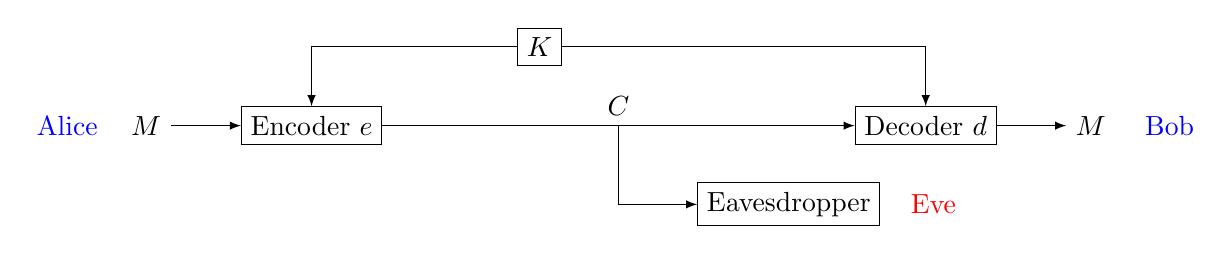
\begin{tikzpicture}
	%\draw (0,0) rectangle (4,4);
	
	\node                       (A)     at (-1,1)   {\Structure{Alice}};
	\node                       (B)     at (13,1)   {\Structure{Bob}};
	\node                       (E)     at (10,0)   {\Important{Eve}};
	
	\node 						(M)		at (0,1)	{$M$};
	\node[draw, left] 			(Enc)	at (3,1) 	{Encoder $e$};
	\node[draw] 				(K) 	at (5,2) 	{$K$};
	\node[draw, right] 			(Dec)	at (9,1) 	{Decoder $d$};
	\node 						(HM)	at (12,1) 	{$M$};
	\node[draw, right] 			(Eve)	at (7,0) 	{Eavesdropper};
	
	\draw[-latex] (M) 	-- (Enc);
	\draw[-latex] (Enc) -- (Dec) node[pos=0.5, above]{$C$};
	\draw[-latex] (Dec)	-- (HM);
	
	\draw[-latex] (K) -| (Enc);
	\draw[-latex] (K) -| (Dec);	
	\draw[-latex] (6,1) |- (Eve);
\end{tikzpicture}
\end{center}

Now we are interested in protecting the contents of the message from eavesdroppers, known as Eve. The message sender, and encoder, is traditionally called Alice.
The receiver, and decoder, is traditionally called Bob.





\paragraph{Notation}

The message $M \in \alphabet{M}$ is known as the \Define{plaintext}. Alice and Bob have some secret information $K \in \alphabet{K}$, known as the \Define{key}.
Alice encrypts using an encryption function $e : \alphabet{M} \times \alphabet{K} \to \alphabet{C}$.
The transmitted sequence
\[
    C = e(M,K) \in \alphabet{C}
\]
is called the \Define{ciphertext}. Bob receives $C$, and decrypts using the decryption function $d : \alphabet{C} \times \alphabet{K} \to \alphabet{M}$. We require that
\[
    d( e(M,K), K ) = M
\]
for all plaintexts $M$. This implies that for a given key $K$, the encryption function is injective:
\[
    e(M_1, K) = e(M_2, K) \implies M_1 = M_2.
\]




\paragraph{Kerchoff's principles}

Clearly, if Eve knows both the decoding algorithm $d$ and the key $K$, then she can decipher the ciphertext. So at least one of the two should be kept secret. Auguste Kerchoffs argued that only the key should be kept secret:
\begin{quote}
    The cipher method must not be required to be secret, and it must be able to fall into the hands of the enemy without inconvenience.
\end{quote}
This is known as \Define{Kerchoff's principle}.

There are three main arguments supporting Kerchoff's principle:
\begin{enumerate}
    \item It is much easier to maintain secrecy of a short key than to keep secret the (more complex) algorithm they are using. (Imagine using encryption to secure the communication between all pairs of employees in some organisation.)
    
    \item If the shared, secret information is ever exposed, then it will be much easier to change a key than to replace an encryption scheme.
    
    \item For large-scale deployment, it is much easier for users to all rely on the same encryption algorithm or software (with different keys) than for everyone to use their own custom algorithm. In fact, it is desirable for encryption schemes to be standardise so that compatibility is ensured by default and users will use a scheme that has undergone public scrutiny without weaknesses being found.
\end{enumerate}

Kerchoff's principle leads us to use cryptosystems whose designs are completely public, instead of trying to rely on ``security by obscurity.''


\paragraph{Breaking a cryptosystem}
The enemy (Eve) is assumed to know the encryption function $e$, the decryption function $d$, and also to have various additional information, such as language statistics etc.
She will certainly have some ciphertext $C$.
All she lacks to decipher to message is the key $K$.

There are three standard forms of attack:
\begin{enumerate}
    \item Ciphertext-only attack.
    
    \item Known-plaintext attack.
Eve is assumed to also have a sample of plaintext and its encryption.

    \item Chosen-plaintext attack.
Eve is able to acquire chosen samples of plaintext/ciphertext pairs.
\end{enumerate}
Current cryptosystems are required to be secure against chosen-plaintext attacks.




\subsection{Examples of cryptosystems}

\paragraph{Early history}
Aeneas Tacticus has a chapter ``On secret messages'' in his classic military manual on the art of war (c. 360BC).
His most secret method was to thread a string through holes in a piece of bone in an order corresponding to the letters of the message.


In the \Important{Caesar cipher}, allegedly used by Julius Caesar, involves shifting all the letters of the alphabet a fixed number of letters later in the alphabet (wrapping from z round to a). For instance, shifting by four characters, ``\texttt{pinkfloyd}'' becomes ``\texttt{tmrojpsch}''.


\paragraph{Substitution cipher}

In the \Define{substitution cipher}, the key is a permutation of the letters of the alphabet:
\begin{align*}
          &\texttt{ABCDEFGHIJKLMNOPQRSTUVWXYZ}\\
       K = \ &\texttt{QWERTYUIOPASDFGHJKLZXCVBNM}
\end{align*}
Encryption is achieved by applying the permutation letter-wise. For instance, using the key above,
\begin{align*}
    M &= \texttt{SENDMORETROOPS}\\
    C &= \texttt{LTFRDGKTZKGGHL}
\end{align*}

This scheme is highly vulnerable to \Important{frequency analysis} for large texts. As we saw earlier, the letter frequencies are heavily biased in text. Since the substitution cipher preserves the character frequencies, the attacker can guess the key by analysing the frequencies in the text. For instance, the most frequent letter in the ciphertext is probably the image of \texttt{E} under the permutation, and so on.




\paragraph{Vigen\`ere cipher}
    
The \Define{Vigen\`ere cipher} is a polyalphabetic substitution cipher, an extension of the Caesar and (simple) substitution ciphers. The key is a sequence of letters, e.g. $K = \texttt{BOTTLEOFRUM}$
The key is repeated until it is as long as the message, and corresponding message and key characters are added (mod 26).
\begin{align*}
    M &= \texttt{THETREASUREISUNDERTHEROCKBYTHETHIRDPALMTREE}\\
    K &= \texttt{BOTTLEOFRUMBOTTLEOFRUMBOTTLEOFRUMBOTTLEOFRU}\\
    C &= \texttt{VWYNDJPYMMRKHOHPJGZZZEQREVKYWKLCVTSJUXRIXWZ}
\end{align*}
If the length of the key is guess right, then the attacker can still use frequency analysis.



\paragraph{Autokey Vig\`enere cipher}
The basic idea is to break the frequency analysis by having a non-repeating key. Again, the key is a sequence of letters e.g. $K = \texttt{BOTTLEOFRUM}$. The key is repeated only once, instead it is augmented to $K^*$ with the start of the message.
\begin{align*}
    M &= \texttt{THETREASUREISUNDERTHEROCKBYTHETHIRDPALMTREE}\\
    K &= \texttt{BOTTLEOFRUM}\\
    K^* &= \texttt{BOTTLEOFRUMTHETREASUREISUNDERTHEROCKBYTHETH}\\
    C &= \texttt{VWYNDJPYMMRCAZHVJSMCWWXVFPCYZYBMAGGACKGBWYM}
\end{align*}

This system was considered unbreakable for nearly 300 years. Then in 1863, a Prussian major discovered that the the length of the keyword can be accurately determined by looking at the separation of repeated digrams. Once the key length is known, frequency analysis can be used to determine the Caesar shift for that set of character positions.

For instance, let us guess a key length of $11$.
Frequency test each letter of alphabet as candidates for first letter of $K$. When we hit \texttt{B} we decode \texttt{T}, use \texttt{T} to decode \texttt{I}, \texttt{I} to get \texttt{O}, \texttt{O} to get \texttt{R}, etc.









\subsection{Perfect cryptosystems}

\paragraph{Perfect cryptosystems}
A cryptosystem is \Define{perfect} if knowledge of the ciphertext $C$ gives absolutely no information about the plaintext $M$.

\begin{theorem}
In a perfect cryptosystem there must be at least as many possible keys as possible plaintexts. 
\end{theorem}

\begin{proof}
Suppose $|\alphabet{K}| < |\alphabet{M}|$ and let $C$ be a ciphertext. Let $d(C)$ denote the set of plaintexts that be decrypted from $C$:
\[
    d(C) = \{M \in \alphabet{M} : \exists K \in \alphabet{K} e(M,K) = C\}.
\]
We then have $d(C) \subseteq \alphabet{M}$. Also, since for every key $K$ encryption is injective, we have $|d(C)| \le |\alphabet{K}| < |\alphabet{M}|$. Thus, $d(C) \subset \alphabet{M}$ and there exists $M^* \in \alphabet{M} \setminus d(C)$: the ciphertext $C$ gives away the information that the plaintext is not $M^*$.
\end{proof}


\paragraph{One-time pad}
In the \Define{one-time pad}, the key length of the Vigen\`ere cipher is extended to be as long as the plaintext. The key characters are generated uniformly at random.
\begin{align*}
    M &= \texttt{THETREASUREISUNDERTHEROCKBYTHETHIRDPALMTREE}\\
    K &= \texttt{BHMNHRPBHQOILQWDBWPQCJNMYPKIPBZPWFZMDFNRBUC}\\
    C &= \texttt{VPRHZWQUCITRELKHGOJYHBCPJRJCXGTXFXDCERALTZH}
\end{align*}

Each character of $C$ is now a uniformly random letter, independently of all others. Thus each ciphertext $C$ is equally likely, no matter what the plaintext $M$ is. The One-time pad is a perfect cryptosystem.

There are two main problems with the one-time pad:
\begin{enumerate}
    \item Key generation. In theory, one would need to generate a very large amount of random characters. Alternatively, one could use a cryptographically secure pseudo-random number generator.
    
    \item Key distribution. The keys are usually not shared amongst only two people, but a whole book of keys is deployed to many agents in the same organisation. This deployment of a large amount of data to many people is not secure in itself.
\end{enumerate}




\subsection{See further}

\paragraph{Enigma}
Mechanical cipher machines came into wide use by World War II. The most famous is the German Enigma machine.

Enigma was a polyalphabetic substitution cipher based on electromechanical rotors that changed the substitution cipher after each letter. The substitution cipher would not repeat for 16900 characters. Probably would have been unbreakable if better procedures had been followed during use.

Work on breaking the Enigma cipher led to major advances in computing, in large part by Alan Turing and Gordon Welchman. 




\subsection{Exercises}

\begin{exercise} \label{exercise:substitution1}
I have used a simple substitution cipher to encode some text; the ciphertext is the file \texttt{ciphertext1.txt}. Compute the letter frequencies in the paragraph. Look up the letter frequencies for common English on the web. Use this knowledge to decipher the paragraph. If it is too much work to compute letter frequencies for the whole paragraph, you could use a short part of the paragraph. Think about how this would affect the results.
\end{exercise}


\begin{exercise} \label{exercise:substitution2}
I did the same with another text to get \texttt{ciphertext2.txt}. This one may be a bit more difficult - the letter frequencies are a bit odd.
\end{exercise}











\section{Symmetric cryptography I: Block ciphers}
\label{sec:12}


An $n$-bit \Define{block cipher} is a function $e : \{0,1\}^n \times \mathcal{K} \to \{0,1\}^n$, such that for each
key $K \in \alphabet{K}$, $e(M,K)$ is an invertible permutation of $\{0,1\}^n$ (the encryption function for $K$).



\subsection{Modes of operations}

A block cipher is not a cryptosystem per se. It is only used to encrypt a particular block of data. It forms a cryptosystem when the mode of operation is specified.

\paragraph{Electronic Codebook} 
The simplest of the encryption modes is the electronic codebook (\Define{ECB}) mode (named after conventional physical codebooks). The message is divided into blocks, and each block is encrypted separately.

\begin{center}
    \includegraphics[width=15cm]{Cryptography/ECB_encryption.png}
    \includegraphics[width=15cm]{Cryptography/ECB_decryption.png}
\end{center}


The disadvantage of this method is a lack of diffusion. Because ECB encrypts identical plaintext blocks into identical ciphertext blocks, it does not hide data patterns well Therefore, global patterns across the plaintext are still kept in the ciphertext. As such, ECB is not recommended for use in cryptographic protocols.


\begin{center}
    \includegraphics[width=5cm]{Cryptography/Tux.jpg} \hspace{2cm} \includegraphics[width=5cm]{Cryptography/Tux_ecb.jpg}
\end{center}

\paragraph{Cipher Block Chaining}
In the cipher block chaining (\Define{CBC}) mode of operation, each block of plaintext is XORed with the previous ciphertext block before being encrypted. This way, each ciphertext block depends on all plaintext blocks processed up to that point. To make each message unique, an initialization vector (\Important{IV}) must be used in the first block.


\begin{center}
    \includegraphics[width=15cm]{Cryptography/CBC_encryption.png}
    \includegraphics[width=15cm]{Cryptography/CBC_decryption.png}
\end{center}


\paragraph{Cipher Feedback}
The cipher feedback (\Define{CFB}) mode, in its simplest variation is using the entire output of the block cipher. In this variation, it is very similar to CBC, makes a block cipher into a self-synchronizing stream cipher. 



\begin{center}
    \includegraphics[width=15cm]{Cryptography/CFB_encryption.png}
    \includegraphics[width=15cm]{Cryptography/CFB_decryption.png}
\end{center}












\subsection{Data Encryption Standard}

\paragraph{Feistel cipher}
A \Define{Feistel cipher} is an iterated cipher mapping a $2t$-bit plaintext $(L_0,R_0)$, for
$t$-bit blocks $L_0$ and $R_0$, to a ciphertext $(R_r, L_r)$, through an $r$-round process where $r \ge 1$.

For $1 \le i \le r$, round $i$ maps $(L_{i-1}, R_{i-1}), K_i \to (L_i,R_i)$ as follows: 
\begin{align*}
    L_i &= R_{i-1},\\
    R_i &= L_{i-1} \oplus f(R_{i-1}, K_i),
\end{align*}
where each subkey $K_i$ is derived from the cipher key $K$.


Typically in a Feistel cipher, $r \ge 3$ and often is even. The Feistel structure specifically
orders the ciphertext output as $(R_r, L_r)$ rather than $(L_r,R_r)$; the blocks are exchanged
from their usual order after the last round. Decryption is thereby achieved using the same
$r$-round process but with subkeys used in reverse order, $K_r$ through $K_1$.

The $f$ function of the Feistel cipher need not be invertible to allow inversion of
the Feistel cipher. We illustrate that successive rounds of a Feistel cipher operate on alternating halves of the ciphertext, while the other remains constant. 

\begin{center}
    \includegraphics[width=10cm]{Cryptography/feistel.png}
\end{center}

The Data Encryption Standard (\Important{DES}) is a Feistel cipher which processes plaintext blocks of $n = 64$ bits, producing $64$-bit ciphertext blocks. 

\paragraph{DES key schedule}
The effective size of the secret key $K$ is $k = 56$ bits. More precisely, the input key $K$ is specified as a $64$-bit key, $8$ bits of which (bits $8, 16, \dots, 64$) are used as odd-parity bits:
\[
    k_8 = k_1 \oplus k_2 \oplus k_3 \oplus k_4 \oplus k_5 \oplus k_6 \oplus k_7 \oplus 1
\]
(and so on for $k_{16}, k_{24}, \dots, k_{64}$). The $2^{56}$ keys implement (at most) $2^{56}$ of the $2^{64}!$ possible bijections on $64$-bit blocks. A widely held belief is that the parity bits were introduced to reduce the effective key size from $64$ to $56$ bits, to intentionally reduce the cost of exhaustive key search by a factor of $256$.\\
~\\
Algorithm DES key schedule\\
INPUT: 64-bit key $K = k_1 \dots k_{64}$.\\
OUTPUT: sixteen $48$-bit keys $K_i$, $1 \le i \le 16$.\\
1. Define $v_i$, $1 \le i \le 16$ as follows: $v_i = 1$ for $i \in \{1, 2, 9, 16\}$; $v_i = 2$ otherwise.\\
2. $(C_0,D_0) \gets PC1(K)$. \\
3. For $i$ from $1$ to $16$, let $X^{\gets v}$ denote $X$ shifted cyclically to the left $v$ times, then do
\begin{align*}
    C_i &\gets C_{i-1}^{\gets v_i},\\
    D_i &\gets D_{i-1}^{\gets v_i},\\
    K_i &\gets PC2(C_i,D_i).
\end{align*}


\begin{tabular}{ccccccc}
\multicolumn{7}{c}{$PC1$}\\
57 & 49 & 41 & 33 & 25 & 17 & 9\\
1 & 58 & 50 & 42 & 34 & 26 & 18\\
10 & 2 & 59 & 51 & 43 & 35 & 27\\
19 & 11 & 3 & 60 & 52 & 44 & 36\\
\multicolumn{7}{c}{above for $C_i$; below for $D_i$}\\
63 & 55 & 47 & 39 & 31 & 23 & 15\\
7 & 62 & 54 & 46 & 38 & 30 & 22\\
14 & 6 & 61 & 53 & 45 & 37 & 29\\
21 & 13 & 5 & 28 & 20 & 12 & 4
\end{tabular}
\hfill
\begin{tabular}{cccccc}
\multicolumn{6}{c}{$PC2$}\\
14 & 17 & 11 & 24 & 1 & 5\\
3 & 28 & 15 & 6 & 21 & 10\\
23 & 19 & 12 & 4 & 26 & 8\\
16 & 7 & 27 & 20 & 13 & 2\\
41 & 52 & 31 & 37 & 47 & 55\\
30 & 40 & 51 & 45 & 33 & 48\\
44 & 49 & 39 & 56 & 34 & 53\\
46 & 42 & 50 & 36 & 29 & 32
\end{tabular}



\paragraph{Feistel function for DES}

Encryption proceeds in $16$ stages or rounds. From the input key $K$, sixteen $48$-bit
subkeys $K_i$ are generated, one for each round. Within each round, $8$ fixed, $6$-to-$4$ bit substitution mappings (S-boxes) $S_i$, collectively denoted $S$, are used. The $64$-bit
plaintext is divided into $32$-bit halves $L_0$ and $R_0$. Each round is functionally equivalent, taking $32$-bit inputs $L_{i-1}$ and $R_{i-1}$ from the previous round and producing $32$-bit outputs
$L_i$ and $R_i$ for $1 \le i \le 16$, as follows:
\begin{align*}
    L_i &= R_{i-1},\\
    R_i &= L_{i-1} \oplus f(R_{i-1}, K_i),
\end{align*}
where 
\[
    f(R_{i-1}, K_i) = P( S( E( R_{i-1} ) \oplus K_i ) ).
\]
Here $E$ is a fixed expansion permutation mapping $R_{i-1}$ from $32$ to $48$ bits. $P$ is another fixed permutation on $32$ bits. The tables below give $E$ and $P$, that is 
\begin{align*}
    E(r_1, r_2, r_3, \dots, r_{31}, r_{32}) &= (r_{32}, r_1, r_2, \dots, r_{32}, r_1)\\
    P(t_1, t_2, t_3, \dots, t_{31}, t_{32}) &= (t_{16}, t_7, t_{20}, \dots, t_4, t_{25}). 
\end{align*}

\begin{tabular}{cccccc}
\multicolumn{6}{c}{$E$}\\
32 & 1 & 2 & 3 & 4 & 5\\
4 & 5 & 6 & 7 & 8 & 9\\
8 & 9 & 10 & 11 & 12 & 13\\
12 & 13 & 14 & 15 & 16 & 17\\
16 & 17 & 18 & 19 & 20 & 21\\
20 & 21 & 22 & 23 & 24 & 25\\
24 & 25 & 26 & 27 & 28 & 29\\
28 & 29 & 30 & 31 & 32 & 1
\end{tabular}
\hfill
\begin{tabular}{cccc}
\multicolumn{4}{c}{$P$}\\
16 & 7 & 20 & 21\\
29 & 12 & 28 & 17\\
1 & 15 & 23 & 26\\
5 & 18 & 31 & 10\\
2 & 8 & 24 & 14\\
32 & 27 & 3 & 9\\
19 & 13 & 30 & 6\\
22 & 11 & 4 & 25
\end{tabular}

The $S_i$ S-boxes are given in the table below. The \Important{S-boxes} are the only \Important{nonlinear} components of the encryption, and as such are the crucial component of its security. In DES, the S-boxes were introduced as lookup tables, with no indication of why they were chosen like that in the first place.

They are applied as follows. First, let $B_i = (b_1, b_2, b_3, b_4, b_5, b_6)$, then $\text{row} = 2b_1 + b_6$, $\text{column} = 8b_2 + 4b_3 + 2b_4 + b_5$. Then look-up the table and write the entry in binary (on four bits). Four instance, here is how to compute $S_1(011011)$:
\begin{align*}
    B &= 011011\\
    \text{row} &= 1\\
    \text{column} &= 13\\
    S_1[1,13] &= 5 = 0101.
\end{align*}

\begin{center}
    \includegraphics[width=15cm]{Cryptography/dess.png}
\end{center}



Here is how to compute the Feistel function $f$:
\begin{enumerate}
    \item Expand $R_{i-1} = r_1 r_2 \dots r_{32}$ from $32$ to $48$ bits using $E$:
$T \gets E(R_{i-1})$. (Thus $T = r_{32} r_1 r_2 \dots r_{32} r_1$.)

    \item $T \gets T \oplus K_i$. Represent $T$ as eight $6$-bit character strings: $(B_1, \dots ,B_8) = T$.
    
    \item $T \gets (S_1(B_1), S_2(B_2), \dots, S_8(B_8))$.
    
    \item $T \gets P(T)$.
\end{enumerate}

\begin{center}
    \includegraphics[width=10cm]{Cryptography/desf.png}
\end{center}





\paragraph{The whole DES algorithm}
An initial bit permutation ($IP$) precedes the first round; following the last round, the left and right halves are exchanged and, finally, the resulting string is bit-permuted by the inverse of $IP$, sometimes referred to as final bit permutation $FP = IP^{-1}$. Similarly to the tables above, we have
\begin{align*}
    IP(m_1, m_2, \dots, m_{64}) &= (m_{58}, m_{50}, \dots, m_7)\\
    FP(b_1, b_2, \dots, b_{64}) &= (b_{40}, b_8, \dots, b_{25}).
\end{align*}

\begin{tabular}{cccccccc}
\multicolumn{8}{c}{$IP$}\\
58 & 50 & 42 & 34 & 26 & 18 & 10 & 2\\
60 & 52 & 44 & 36 & 28 & 20 & 12 & 4\\
62 & 54 & 46 & 38 & 30 & 22 & 14 & 6\\
64 & 56 & 48 & 40 & 32 & 24 & 16 & 8\\
57 & 49 & 41 & 33 & 25 & 17 & 9 & 1\\
59 & 51 & 43 & 35 & 27 & 19 & 11 & 3\\
61 & 53 & 45 & 37 & 29 & 21 & 13 & 5\\
63 & 55 & 47 & 39 & 31 & 23 & 15 & 7
\end{tabular}
\hfill
\begin{tabular}{cccccccc}
\multicolumn{8}{c}{$FP$}\\
40 & 8 & 48 & 16 & 56 & 24 & 64 & 32\\
39 & 7 & 47 & 15 & 55 & 23 & 63 & 31\\
38 & 6 & 46 & 14 & 54 & 22 & 62 & 30\\
37 & 5 & 45 & 13 & 53 & 21 & 61 & 29\\
36 & 4 & 44 & 12 & 52 & 20 & 60 & 28\\
35 & 3 & 43 & 11 & 51 & 19 & 59 & 27\\
34 & 2 & 42 & 10 & 50 & 18 & 58 & 26\\
33 & 1 & 41 & 9 & 49 & 17 & 57 & 25
\end{tabular}
~\\
~\\
Algorithm Data Encryption Standard (DES)\\
INPUT: plaintext $M = (m_1, \dots, m_{64})$; $64$-bit key $K = (k_1, \dots, k_{64})$.\\
OUTPUT: $64$-bit ciphertext block $C = (c_1, \dots, c_{64})$. \\
1. Compute sixteen $48$-bit round keys $K_i$ from $K$.\\
2. $(L_0, R_0) \gets IP(M)$. \\
3. for $i$ from $1$ to $16$, compute $L_i$ and $R_i$ as above.\\
4. $B = (b_1, b_2, \dots, b_{64}) \gets (R_{16}, L_{16})$. \\
5. $C \gets FP(B)$.


Decryption involves the same key and algorithm, but with subkeys applied to the internal rounds in the reverse order.



\begin{center}
    \includegraphics[width=5cm]{Cryptography/des.png}
\end{center}





\subsection{See further}

\paragraph{Other modes of operation}
A few other modes of operation have been proposed. We can mention Output feedback (\Define{OFB}), similar to CFB, but where the output of the encryption block function (rather than the ciphertext) serves as the feedback. Another related mode of operation is Counter (\Define{CTR}), which encrypts successive values of a counter.


\paragraph{AES}
The Advanced Encryption Standard (\Define{AES}) was introduced in 2002 in order to replace DES as the new standard for block ciphers. Unlike DES, where some details were kept secret, AES was selected using a competition where all the algorithms had to explain all the details and design choices.

Overview of AES: 128 bit message block represented as a 4 by 4 array of bytes. It applies 10 rounds of: 
\begin{itemize}
    \item S-box transformation
    \item ShiftRows
    \item MixColumns
    \item Add sub-key.
\end{itemize}
The first three operations are all fixed. The fourth one is the only use of the key. Again, the S-box substitutions are the key non-linear element. The rest helps diffuse uncertainty.



\subsection{Exercises}


\begin{exercise} \label{exercise:feistel}
By hand, encrypt the following plaintext $M = 01110001$ ($8$ bits) using a Feistel cipher with 4 rounds and function
\[
    f(x_1, x_2, x_3, x_4) = x_1x_2 + x_2x_3 + x_3x_4 + x_4x_1 \mod 2. 
\]
For simplicity, we apply $f$ to $R_{i-1} \oplus K_i$, so that the actual Feistel function is
\[
f(r_1, r_2, r_3, r_4, k_1, k_2, k_3, k_4) = (r_1 + k_1)(r_2 + k_2) + (r_2 + k_2)(r_3 + k_3) + (r_3 + k_3)(r_4 + k_4)  + (r_4 + k_4) (r_1 + k_1) \mod 2.
\]
You can choose anything you want for the four $4$-bit subkeys $K_1, K_2, K_3, K_4$.

Decrypt the ciphertext and verify that you get the right plaintext.
\end{exercise}


\begin{exercise} \label{exercise:weak_keys}
A DES weak key is a key $K$ such that $E_K(E_K(x)) = x$ for all $x$, i.e., defining
an involution.
Verify that the four keys in the table below are indeed weak keys. I give $K$ in hexadecimal and the corresponding $C_0$ and $D_0$; note that the subkeys are easy to determine in those cases!\\
~\\
\begin{tabular}{lll}
weak key (hexadecimal) & $C_0$ & $D_0$\\
0101 0101 0101 0101 & $0\dots0$ & $0\dots0$\\
FEFE FEFE FEFE FEFE & $1\dots1$ & $1\dots1$\\
1F1F 1F1F 0E0E 0E0E & $0\dots0$ & $1\dots1$\\
E0E0 E0E0 F1F1 F1F1 & $1\dots1$ & $0\dots0$
\end{tabular}

Those actually are the only weak keys of DES.
\end{exercise}









\section{Symmetric cryptography II: Cryptanalysis}
\label{sec:13}


\subsection{Weaknesses of DES}


\paragraph{Attacking DES}
Even in 1977 the key size (56 bits) was considered 'low'.
The NSA 'encouraged' the dropping of key size from 128 to 56 bits at the time - could they mount a brute force attack even then?
Proposed machines to break DES by brute force are:
\begin{itemize}
    \item 1977. Diffie and Hellman outline a \$20million machine to crack DES in 1 day.
    
    \item 1993. Wiener proposed a \$1million machine to crack DES in 7 hours.
    
    \item 1997. RSA corp. sponsored a competition to crack DES. It was won by a program using downtime of home PCs connected to the internet. 1 PC would have taken 2285 years to search the key space. They had 78,000 PCs signed up by the time they found the key, after searching 1/4 of the key space.
    
    \item 1998. The EFF built a \$250,000 machine that cracks DES in 2 days.
    
    \item 2006. A \$10,000 machine (COPACOBANA) is built from off-the-shelf kit that cracks DES in less than a week.
\end{itemize}



\paragraph{Key size}
If our key size is 56 bits, there are $2^{56}$ possible keys and testing randomly we would expect to test about $2^{55}$ before we cracked it. Suppose we can test a billion ($2^{30}$) possible keys per second. There are $2^{25}$ seconds per year, so we test about $2^{55}$ keys per year. 

The amount of time required to break a 128-bit key is very much greater. About 
\[
    2^{127} = 170,141,183,460,469,231,731,687,303,715,884,105,728
\]
possibilities must be checked. A device that checks a billion billion keys ($2^{60}$) per second would require about $10^{13}$ years to exhaust the key space. This is a thousand times longer than the age of the universe.

AES permits the use of $256$-bit keys. Breaking a symmetric $256$-bit key by brute force requires $2^{128}$ times more computational power than a $128$-bit key. A device that could check a billion billion ($10^{18}$) AES keys per second would require about $10^{51}$ years to exhaust the 256-bit key space.





\paragraph{TripleDES and DES-X}
Two main variants of DES were introduced to increase the key space/size.

\Define{TripleDES}: Take three DES keys $K_1$, $K_2$, $K_3$. Encrypt a block $M$ as 
\[
    C = e( d( e(M, K_1), K_2), K_3), 
\]
where $e$ is the standard DES encryption, and $d$ is the standard DES decryption. The key size is now $3 \times 56 = 168$ bits, but effective security is only ca. 112 bits due to meet-in-the-middle attacks. TripleDES is backwards compatible taking $K_1 = K_2 = K_3$.

\Define{DES-X}: Take a DES key $K$, and two supplementary 64 bit keys $K_1$, $K_2$. Encrypt a block $M$ as 
\[
    C = K_2 + e( M + K_1, K ).
\]
The  Key size is now 184 bits, but effectively ca. 119 bits. Since only one DES encryption is performed, this is much faster than TripleDES.



\subsection{Cryptanalysis of block ciphers}

\paragraph{Meet-in-the-middle}
Suppose we are using a $k$-bit cryptosystem with encryption function $e$ and decryption function $d$. We decide to increase security by encrypting twice as follows.: choose two keys $K_1$ and $K_2$ each of $k$ bits, and then do
\[
    C = e( e(M,K_1) , K_2).
\]

The effective security is not $2k$ bits. Suppose a plaintext/ciphertext pair $M$, $C$ is publicly known. The attacker could compute a table of $e(M,K)$ for all $2^k$ possible keys $K$. Then she can compute $d(C,K')$ for all possible keys $K'$, checking for a match:
\[
    e(M,K) = d(C,K'). 
\]
This gives a pair of keys such that 
\[ 
    e( e(M,K) , K') = C.
\]
The total encryptions/decryptions performed is $2^{k+1}$. The space required is only enough to store $2^k$ keys and text snippets.


\paragraph{Linear cryptanalysis}
Linear cryptanalysis is quite involved, so we only give the basic ideas.

Suppose that it is possible to find a probabilistic linear relationship between a subset of plaintext bits and a subset of state bits immediately after the substitutions performed in the last round, In other words, there exists a subset of bits whose exclusive-or behaves in a \Important{non-random fashion} (it takes the value $0$ with probability bounded away from $1/2$).

Now assume that an attacker has a large number of plaintext-ciphertext pairs for the same unknown key $K$ (i.e. this is a known-plaintext attack). For each of the plaintext-ciphertext pairs, we begin to decrypt the ciphertext, using all possible candidate keys for the last round of the cipher. We keep track of when the linear relationship does hold for each key. At the end of this process, we hope that the candidate key with the most biased count (furthest away from $1/2$ of the number of pairs) contains the correct value for these bits.

Performing a linear attack involves computing a linear approximation of the S-boxes. Therefore, a secure S-box must have a high \Important{nonlinearity}, defined as the distance to any linear or affine function.

\Define{Linear cryptanalysis} was introduced by Matsui in 1994. He actually performed a linear attack on DES the same year. The linear cryptanalysis of DES is a known-plaintext attack using $2^{43}$ plaintext-ciphertext pairs, all of which are encrypted using the same unknown key. This actual attack did not have any impact on the security of DES due to the large number of pairs required. Nonetheless, AES was designed to resit linear cryptanalysis.


\paragraph{Differential cryptanalysis}
Differential cryptanalysis is similar to linear cryptanalysis in many respects. The main difference is that it involves comparing the \Important{xor of two inputs} to the xor of the corresponding two outputs. 

Differential cryptanalysis is a chosen-plaintext attack. The attacker has a large number of tuples $(x, x^*, y, y^*)$ (input, input, output, output), where the value $x' = x \oplus x^*$ is fixed and $x$ and $x^*$ are encrypted using the same key.

\Define{Differential cryptanalysis} was discovered in the late 1980s by Biham and Shamir. They noted that DES was resistant to differential cryptanalysis. In fact, IBM and the NSA knew about differential cryptanalysis since the mid-70s and hence designed DES to be robust against this sort of attack.



\subsection{See further}

\paragraph{Design of S-boxes}
Mathematically, an S-box is a function $\{0,1\}^n \to \{0,1\}^m$ for some $m$ and $n$. It can then be viewed as a tuple of $m$ Boolean functions $(s_1, \dots, s_m)$, where $s_i : \{0,1\}^n \to \{0,1\}$ is a Boolean function.

The security of the block cipher depends on the S-box, and hence on its component Boolean functions. As such, different parameters of Boolean functions have been introduced: nonlinearity, balancedness, resiliency, correlation immunity, algebraic degree, etc.





\subsection{Exercises}

\begin{exercise}
Perform a meet-in-the-middle attack on the simple Feistel cipher of Exercise \ref{exercise:feistel}. (You can choose the solution of that exercise as your publicly known plaintext-ciphertext pair.)
\end{exercise}






\section{RSA I: The system}
\label{sec:14}


\subsection{Public-key cryptography}

\paragraph{One-way functions}
A function $f$ is said to be a \Define{one-way function} if:
\begin{enumerate}
    \item For all inputs $x$ it is easy to compute $f(x)$.

    \item Given some (random) $y$, it is hard to find an $x$ such that $y = f(x)$. 
\end{enumerate}

By easy, we usually mean that it may be computed in time polynomial in $\log x$. Hardness is not so easy to define. At first, you may want inverting $f$ to be an NP-hard problem. But note that NP-hardness is a worst case criterion; random cases, or the majority of cases may still be easy (Knapsack encryption suffers from that drawback). Also, hardness is time dependent: what was in feasible in 1977 is relatively easy today. The minimum requirement for hardness is that there is no known efficient algorithm that works on random instances.




\paragraph{One-way functions}
    
We will look at two candidate one-way functions: multiplication and exponentiation modulo a prime. In this lecture, we focus on multiplication.

\begin{description}
\item [Multiplication] Given two integers $a$, $b$, it is easy (polynomial time) to compute the product $ab$.

\item[Inverting (factoring)] Given a large integer $c$, is it difficult to find integers $a$, $b$ such that $ab = c$?
\end{description}

Not in general. If you pick $a$, $b$ randomly then each is even with probability $1/2$. So $c = a \cdot b$ is even with probability $3/4$. You can often return $c = 2 \cdot (c/2)$.
Better to pick two $k$ bit primes, $a$, $b$. Now it is usually hard to invert.
The decision problem (Does $c$ have a factor less than $m$?) is not thought to be in P. It is in both NP and co-NP (given a prime factorisation of $c$ you can check both membership and non-membership). The best known algorithm (general number field sieve), for an $n$ bit number runs in time 
\[
    \exp \{ (1.92 + o(1)) (\ln n)^{1/3} (\ln \ln n)^{2/3} \}. 
\]





\paragraph{Public-key cryptography}
A \Define{trapdoor function} is a one-way function that can be easily inverted with a secret key. A public-key cryptosystem uses a trapdoor function as follows:
\begin{enumerate}
    \item Alice encrypts her message $M$, using a one-way function $f$: $C = f(M)$.

    \item Bob has a secret method of opening the trapdoor and inverting $f$.

    \item Even if Eve intercepts $f(M)$, she cannot invert without knowing Bob's secret trapdoor.
\end{enumerate}
Trapdoor functions were first proposed by James Ellis at GCHQ in 1969. The first public key cryptosystem was developed by Clifford Cocks, also at GCHQ, in 1973. Both developments remained secret until 1997.



\paragraph{RSA cryptosystem}
Rivest, Shamir and Adleman rediscovered, and published, Cocks' scheme in 1977. 
It relies on the difficulty of factoring for security.

\begin{description}
\item[Key generation]~
\begin{enumerate}
    \item Bob chooses two large primes $p$ and $q$.

    \item Bob computes the public modulus $n = pq$, and the public exponent $e$ co-prime to $\phi(n) = (p-1)(q-1)$. ($e< \phi(n)$.)

    \item Bob publishes his public key $(n,e)$.
    
    \item His private key is the unique integer $d$ such that $ed = 1 \mod \phi(n)$.
\end{enumerate}

\item [Encryption]~
\begin{enumerate}
    \item Alice breaks her message into blocks so that each block $M$ satisfies $M<n$.

    \item Alice encrypts $M$ as $C = M^e \mod n$.
\end{enumerate}

\item[Decryption]~
\begin{enumerate}
    \item Bob can decrypt using $C^d = M \mod n$.
\end{enumerate}
\end{description}


\paragraph{Proof that RSA works}
The correctness of decryption is nontrivial. It follows from this simple number theoretic result, which can be viewed as a simple case of Lagrange's theorem on the order of subgroups of a finite group.

\begin{theorem}
For any integer $n$ and any $a \in \Z_n^*$,
\[
    a^{\phi(n)} = 1 \mod n.
\]
\end{theorem}
Therefore, the decryption is correct:
\[
    C^d = M^{ed} = M^{ed + k \phi(n)} = M \mod n.
\]


\paragraph{Computing time of RSA}
All the operations (key generation, encryption and decryption) are done in expected polynomial time.

Primality testing is very fast using randomised algorithms, and possible using a deterministic polynomial time algorithm. If we select random odd $k$-bit numbers, we expect to test polynomially many before we find a prime.

Computing $n = pq$ and $\phi(n) = (p-1)(q-1)$ is simple multiplication.

Finding $e$ by random sampling and testing (Euclid's Algorithm), we expect to take polynomially many tests. We can also pick $e$ to be a prime number, then we just need to check it does not divide $\phi(n)$. In practice, we often use the prime number
\[
    e = 65537 = 2^{16}+1.
\]
Finding $d$ is again \Important{Euclid's Algorithm}. Encryption and decryption can be achieved by \Important{repeated squaring}.



\paragraph{Generating random prime numbers}
In practice, one uses the \Important{Miller-Rabin primality test}. It is a yes-biased Monte Carlo algorithm, that is it always give an answer, and never returns ``$n$ is composite'' when $n$ is actually prime. The algorithm runs very fast. The probability of getting it wrong is exponentially small. 



\paragraph{TLS}
Amongst the many applications of RSA, let us mention Transport Layer Security (\Define{TLS}). This is the newer version of SSL, used as the protocol for secure websites (https). Here is a massively reduced summary: 
\begin{enumerate}
	\item Client contacts server and they agree to use the highest level cryptography suite they both know.
	
	\item The client generates a random number and communicates it to the server using public key cryptography (RSA) and the server's public key.
	
	\item The server and client both compute a secret master key from the random number.
	
	\item The master key is used to communicate using symmetric cryptography (AES).
\end{enumerate}
Why? Because symmetric cryptography is about 1000 times faster than RSA.




\subsection{See further}

\paragraph{The Rabin cryptosystem}
RSA is not the only publick-key cryptosystem based on the complexity of factoring. Another example is the \Define{Rabin cryptosystem}, described below.
\begin{description}
    \item[Key generation] Let $n = pq$, where $p$ and $q$ are primes and $p,q = 3 \mod 4$. Then $n$ is the public key, while $(p,q)$ is the private key.
    
    \item[Encryption] Let $x \in \Z_n^*$, then
    \[
        e(x) = x^2 \mod n.
    \]
    
    \item[Decryption] Let $y \in \Z_n^*$, then
    \[
        d(x) = \sqrt{y} \mod n.
    \]
\end{description}
(The restriction $p,q = 3 \mod n$ can actually be omitted.)

The one main drawback of the Rabin cryptosystem is that encryption is not injective. Indeed, any ciphertext $y$ has four possible square roots, and hence corresponds to four possible plaintexts! For instance, let $p = 7$, $q = 11$, $y = 23$. Then a bit of algebra shows that
\[
    10^2, 67^2, 32^2, 45^2 = 23 \mod 77.
\]

\subsection{Exercises}

\begin{exercise} \label{exercise:rsa}
Alice and Bob decide to communicate using RSA. Bob picks primes $p = 5$ and $q = 13$, and public exponent $e = 19$.
\begin{enumerate}
    \item What information does Bob publish as his public key? Give the specific values from this example.

    \item What information comprises Bob's private key? Compute it in this example.
    
    \item What is the process for Alice to send a message to Bob? Alice first coverts each character into a number  (as given in the character - number conversion table attached). She then encrypts each number using Bob's public information, and converts it back to a character to send to Bob. Illustrate how she would encrypt the message "Hell".
    
    \item Explain the process for Bob to decrypt messages he receives and decrypt the message ':Uo'.
    
    \item What would the encryption of the numbers 0, 1 and 64 be? Why aren't they used in the character conversion table?
\end{enumerate}


\begin{tabular}{cccccccccccccccccccc}
0 & 1 & 2 & 3 & 4 & 5 & 6 & 7 & 8 & 9 & 10 & 11 & 12 & 13 & 14 & 15 & 16 & 17 & 18 & 19\\
- & - & \textvisiblespace & \return & A & B & C & D & E & F & G & H & I & J & K & L & M & N & O & P\\
20 & 21 & 22 & 23 & 24 & 25 & 26 & 27 & 28 & 29 & 30 & 31 & 32 & 33 & 34 & 35 & 36 & 37 & 38 & 39\\
Q & R & S & T & U & V & W & X & Y & Z & a & b & c & d & e & f & g & h & i & j \\
40 & 41 & 42 & 43 & 44 & 45 & 46 & 47 & 48 & 49 & 50 & 51 & 52 & 53 & 54 & 55 & 56 & 57 & 58 & 59\\
k & l & m & n & o & p & q & r & s & t & u & v & w & x & y & z & . & , & ? & !\\
60 & 61 & 62 & 63 & 64\\
: & ; & ' & \tab & -
\end{tabular}
\end{exercise}




\section{RSA II: Cryptanalysis}
\label{sec:15}
\subsection{Vulnerabilities of RSA}

\paragraph{General vulnerabilities}

Due to its popularity, RSA has been the subject of much research trying to break the cryptosystem.

Several schemes are known for attacking the system, which perform well if special conditions are met, for instance:
\begin{itemize}
    \item Primes $p$ and $q$ are 'too close' (searching from $\sqrt{n}$ up to $(p+q)/2$ reveals a factor).
    
    \item If $d$ is too small $(< n^{0.25})$, then $d$ can be recovered from $(n,e)$.
    
    \item Sending the same message to different people with the same $e$ is insecure.
\end{itemize}

No scheme for cracking RSA in general, except by factoring $n$, is known.


\paragraph{Other issues}
Problem of non-random messages: If you only send a limited range of messages, Eve can try encrypting each to see which gives the intercepted cryptogram. For instance, if you always send 'Transfer X pounds into my account' or 'My 3-digit card security code is X'.

This is why Alice should always pad messages with random bits.



\subsection{Factorisation algorithms}

\paragraph{Trial division}
The naive factoring algorithm, called \Define{trial division}: ``check all numbers $p$ up to $\sqrt{n}$ to see if $p \divides n-1$'' runs in exponential time. Indeed, the size of the input is $\log n$, while the algorithm would run in $\Omega(\sqrt{n}) = \Omega( c^{\log n} )$ for some constant $c$. There are no polynomial time algorithms known for factoring, but below we present three algorithms that can be much more efficient than the naive factoring algorithm.

\paragraph{Pollard's $p-1$ algorithm}

\Define{Pollard's $p-1$ algorithm} has two inputs: the odd integer $n$ to be factored, and a prescribed bound $B$.


\begin{algorithm}[H]
\caption{Pollard $p-1$ factoring algorithm$(n,B)$}
\begin{algorithmic}[1]
	\State{$a \gets 2$}
	\For{$j \gets 2$ to $B$}
	    \State{$a \gets a^j \mod n$}
    \EndFor
    \State{$d \gets \gcd(a-1, n)$}
    \If{$1 < d < n$}
        \State{\Return{$d$}}
    \Else{}
        \State{\Return{"failure"}}
    \EndIf
\end{algorithmic}
\end{algorithm}

Here's a simple explanation of why this works. Suppose $p$ is a prime divisor of $n$, and suppose that $p-1$ is \Define{$B$-smooth}: $r \le B$ for every prime power $r \divides (p-1)$. That is, we assume that $p-1$ only has \Important{small factors} in its factorisation. For example, the number $2,000$ is $B$-smooth for any $B \ge 125$, since it factors as
\[
    2000 = 2^4 \times 5^3 = 16 \times 125.
\]

\begin{theorem}\label{th:pollard_p-1}
If $p$ is a prime divisor of $n$, and $r \le B$ for every prime power $r \divides (p-1)$, then Pollard's $p-1$ algorithm$(n,B)$ returns $d$, a nontrivial factor of $n$.
\end{theorem}


\begin{proof}
The key idea in the proof is that $p \divides a-1$. Let us prove this now.

At the end of the for loop, we have
\[
    a = 2^{B!} \mod n.
\]
Since $p \divides n$, we have
\[
    a = 2^{B!} \mod p.
\]
Since all the terms in the factorisation of $p-1$ belong to $\{1, 2, 3, \dots, B\}$, we must have
\[
    p-1 \divides 1 \times 2 \times 3 \times \dots \times B = B!.
\]
Say $B! = \gamma (p-1)$. By Fermat's theorem, $a^{p-1} = 1 \mod p$, hence
\[
    a = 2^{B!} \mod p = \left( 2^{p-1} \right)^\gamma \mod p = 1^\gamma \mod p = 1 \mod p.
\]
Thus $p \divides a-1$.

We can now finish the proof. Since $p \divides n$ and $p \divides a-1$, we have $p | d$, where $d = \gcd(a-1,n)$. By definition, $d \divides n$ and, unless $a = 1$, $1 < d < n$; that is, $d$ is a nontrivial divisor of $n$.
\end{proof}

The running time is clearly of the form $O(B \text{poly}(\log n))$. So if $B$ itself is $O(\text{poly}(\log n))$, the $p-1$ algorithm runs in polynomial time. However, it may not work: if $p-1$ has a factor greater than $B$, then the algorithm may return a failure. (Note that if $B = \sqrt{n}$, then the $p-1$ algorithm is sure to work, but that's no improvement compared to the naive algorithm.)

Pollard's $p-1$ algorithm can then be thwarted by constructed $n = pq$ without small factors as follows. First, choose a large prime $p_1$ such that $p = 2p_1 + 1$ is also prime, and similarly a large prime $q_1$ such that $q = 2q_1 + 1$ is also prime. (That task is not actually onerous.) Then the RSA modulus $n = pq$ will be resistant to factorisation using Pollard's $p-1$ algorithm.


\paragraph{Pollard's rho algorithm}

Let $p$ be the smallest prime divisor of $n$. Suppose there exist two integers $x, x' \in \Z_n$ such that $x \ne x'$ and $x = x' \mod p$. Then $p \le \gcd(x-x',n) < n$, hence the gcd is a nontrivial factor of $n$. To find such a collision, one can take a random set $X$ of size $|X| \approx 1.17 \sqrt{p}$: by the birthday paradox, we would find a collision with probability $50\%$. However, we would need to compute $\Theta(|X|^2) = \Theta(p) = \Theta(\sqrt{n})$ gcds.

The \Define{Pollard rho} algorithm is a clever heuristic to find collisions without that many gcds.Let $f(x)$ be a polynomial with integer coefficients. A popular choice is 
\[
    f(x) = x^2 + 1.
\]
We will presume that the mapping $x \mapsto f(x) \mod p$ behaves like a random mapping. That way we can start with a particular value of $x$, say $x_0$ and search for a collision on its \Important{orbit} $X = \{x_0, x_1, \dots, x_k\}$, where
\[
    x_1 = f(x_0) \mod n, x_2 = f(x_1) = f^2(x_0) \mod n, \dots, x_k = f^k(x_0) \mod n.
\]

There must be a collision somewhere on the orbit. Indeed, the mapping $x \mapsto f(x) \mod n$ is a self-map of $\Z_n$, so there are $i$ and $j$ such that $f^i(x_0) \mod n = f^j(x_0) \mod n$. Therefore, there exist $\lambda$ and $\pi$ such that 
\[
    x_\lambda = x_{\lambda + \pi} \mod p.
\]
We say $\lambda$ is the \Define{pre-period} of $x_0$ and $\pi$ is its \Define{period}. If we draw the directed graph $D = (X \mod p, A)$ with arcs $A = \{ (x_i \mod p, x_{i+1} \mod p) \}$, we get a rho-like shape, hence the name of the algorithm.

Let $i'$ satisfy $i' \ge i$ and $i' = 0 \mod \pi$, then
\[
    x_{2i'} = x_{i'} \mod p.
\]
Consider the sequences $B = (x_0, x_1, x_2, \dots)$ and $C = (x_0, x_2, x_4, \dots)$. We then have $b_{i'} = x_{i'}$ and $c_{i'} = x_{2i'} = b_{i'} \mod p$: we can find a collision simply by following those two sequences. We expect $i'$ to be at most $\sqrt{p}$.

\begin{algorithm}[H]
\caption{Pollard $\rho$ factoring algorithm$(n,x_1)$}
\begin{algorithmic}[1]
	\State{$x \gets x_0$}
	\State{$x' \gets f(x) \mod n$}
	\State{$p \gets \gcd(x-x', n)$}
	\While{$p=1$}
	    \State{$x \gets f(x) \mod n$}
	    \State{$x' \gets f^2(x') \mod n$}
	    \State{$p \gets \gcd(x-x',n)$}
    \EndWhile
    \If{$p < n$}
        \State{\Return{$p$}}
    \Else{}
        \State{\Return{"failure"}}
    \EndIf
\end{algorithmic}
\end{algorithm}

Note that there is a small chance of failure if the collision $x = x' \mod p$ actually satisfies $x = x'$. This occurs with probability roughly $p/n$, which is very small in practice. And in any case, if this occurs, then one can simply re-run the algorithm with a different initial point $x_0$.

\paragraph{Quadratic sieve algorithm}

Given $x,y$ with \Important{$x^2 = y^2 \mod n$} and $x \ne \pm y \mod n$, we obtain
\[
    0 = x^2 - y^2 = (x-y)(x+y) \mod n,
\]
and hence $n | (x-y)(x+y)$. But $n$ neither divides $x+y$ nor $x-y$, thus $\gcd(x-y,n)$ is one of the prime factors of $n$.

The \Define{quadratic sieve} algorithm tries to generate such a pair $x$, $y$. The key idea is to select a sequence of elements $x_i \in \Z_n$ and generate the corresponding sequence of values
\[
    q_i = x_i^2 \mod n.
\]
We choose $x_i = \left\lceil \sqrt{n} \right\rceil + i$ (or some choose a double-indexed sequence $x_{i,j} = \left\lceil \sqrt{jn} \right\rceil + i$) because then $x_i^2 \mod n$ is a small number. In fact, we select a bound $B$ and we only keep the $q_i$'s that are $B$-smooth, so we can factor them efficiently. 

Let $p_1, \dots, p_k$ denote the $k$ prime numbers less than or equal to $B$. We then obtain
\begin{align*}
    q_1 &= x_1^2 \mod n = \prod_{j=1}^k p_j^{e_{1,j}}\\
    q_2 &= x_2^2 \mod n = \prod_{j=1}^k p_1^{e_{2,j}}\\
    \vdots\\
    q_l &= x_l^2 \mod n = \prod_{j=1}^k p_j^{e_{l,j}}.
\end{align*}


The next step is to find a subset of the $\{q_i\}$ whose product is a square (in $\N$). If we take the subset $S$, the product is
\[
    z = \prod_{i \in S} q_i = \prod_{j=1}^k p_j^{\sum_{i \in S} e_{i,j}}.
\]
The number $z$ is a square if and only if $\sum_{i \in S} e_{i,j}$ is an even number for all $j$. Finding an $S$ that satisfies this property is actually easy! (This is based on linear algebra over the binary field $\GF(2)$, we'll look at that stuff in Lecture \ref{sec:23}.) Suppose we find the right $S$, then we obtain
\[
    z = \left( \prod_{i \in S} x_i  \right)^2 \mod n.
\]
This gives us two square roots modulo $n$ of $z$: $x^2 = y^2 = z \mod n$. This pair of square roots may not be valid (we may have $x = \pm y \mod n$), but if we use $l > k+1$, we ensure to have multiple sets $S$ and hence multiple pairs of square roots; heuristically this will yield at least one valid pair.

The running time of the quadratic sieve algorithm depends on $B$. A careful analysis of the number of $B$-smooth numbers yields a subexponential $B = O(c^{\sqrt{\log n \log \log n}})$ and an overall \Important{subexponential running time} of
\[
    O\left( \exp( (1 + o(1)) \sqrt{ \ln n \ln \ln n } ) \right).
\]

\paragraph{State-of-the-art}
The current best algorithm for factoring is the so-called Galois Field Number Sieve. It recently (February 2020) managed to factor the number RSA-250: a 250-digit (829 bits) number $n=pq$. In fact, RSA has a challenge with a list of semiprimes ($n= pq$) of increasing length that people try to factor. The list goes up to a number that's 2048 bits long.


\subsection{See further}

\paragraph{Side-channel attacks}
Another type of attack on RSA and similar systems was discovered by Paul Kocher in 1995. He showed that it is possible to discover the decryption exponent by carefully timing the computation times for a series of decryptions (see \cite[Section 6.2]{TW02} for a review). Even though Kocher's \Important{timing attack} can be thwarted, it was nonetheless a game changer as it opened the way for a new range of so-called \Important{side-channel attacks}, whereby the attacker has access to other kinds of data such as timing, power consumption, memory usage, heat diffusion, etc.


\paragraph{Schor's algorithm}
Integer factorisation can be done in polynomial time... on a quantum computer. \Important{Schor's algorithm} is beyond the scope of this course. However, the threat of quantum computers is taken very seriously. Indeed, NIST are holding a competition to standardise \Important{Post-Quantum Cryptography} (\Define{PQC}), i.e. public-key cryptosystems and signature schemes based on problems which are believed to be secure against quantum attacks. There are two main kinds of post-quantum cryptosystems left: those based on \Important{lattice problems} (Lectures \ref{sec:19} and \ref{sec:20}) and those based on \Important{error-correcting codes} (Lectures \ref{sec:29} and \ref{sec:30}).

\subsection{Exercises}

\begin{exercise}
Apply Pollard's $p-1$ algorithm for $n = 15770708441$ and $B = 175$ to obtain
\[
    n = 135979 \times 115979.
\]
(Yes, you need a computer for this one.)
\end{exercise}


\begin{exercise}
Let $n = 7171$. With $x_0 = 1$, use Pollard's rho algorithm to find the factor $71$ of $n$. (You should get $\gcd(x_{11} - x_{22}, n) = 71$.)
\end{exercise}


























\section{Discrete logarithm cryptography}
\label{sec:16}

\subsection{Diffie-Hellman key exchange}

The \Define{Diffie-Hellman key exchange} (1976) is a mechanism to agree on a secret key by exchanging messages without revealing the actual key value. It is based on the difficulty of \Important{discrete logarithms}.

If $p$ is a prime, then we say $g \in \Z_p^*$ is \Define{primitive mod $p$} (or a generator) if all the elements of $\Z_p^*$ are powers of $g$:
\[
    \{g, g^2 \mod p, g^3 \mod p, \dots, g^{p-1} \mod p = 1  \} = \{1, 2, \dots, p-1 \}.
\]
It is easily shown that there are $\phi(p-1)$ primitive elements mod $p$, where $\phi(n)$ is Euler's totient function.

Here is the protocol.
\begin{enumerate}
    \item Alice and Bob publicly agree a large prime $p$ and a primitive element $g$. 

    \item Alice and Bob choose private keys $a$ and $b$ (between $2$ and $p-2$).
    
    \item Alice computes 
    \[
        A = g^a \mod p,
    \]
    and sends $A$ to Bob.
    
    \item Bob computes 
    \[
        B = g^b \mod p,
    \]
    and sends $B$ to Alice.
    
    \item Alice computes the shared secret key 
    \[
        K = B^a \mod p.
    \]
    
    \item Bob computes $K$ as 
    \[
        K = A^b \mod p.
    \]
\end{enumerate}


Alice and Bob know the same $K$, since 
\[
    A^b = (g^a)^b = g^{ab} = (g^b)^a = B^a.
\]
Eve only knows $A$, $B$, $p$ and $g$. If Eve could compute discrete logarithms easily, then she could obtain (for instance): $a = \log_g A$ and then $K = B^a \mod p$.


\subsection{The ElGamal cryptosystem}


Let $p$ be a large prime number, and let $g \in \Z_p^*$ be a primitive element. Let $\mathcal{M} = \Z_p^*$, $\mathcal{C} = \Z_p^* \times \Z_p^*$.

\begin{description}
\item[Key generation]
    \begin{enumerate}
        \item Let $A = g^a \mod p$ for some $a$
        
        \item Public key: $(p, g, A)$
        
        \item Private key: $a$
    \end{enumerate}

\item[Encryption] Choose a secret random number $k \in \Z_{p-1}$, then
\begin{align*}
    e(x, k) &= (y_1, y_2),\\
    y_1 &= g^k \mod p\\
    y_2 &= x A^k \mod p.
\end{align*}


\item[Decryption]
\[
    d(y_1,y_2) = y_2 (y_1^a)^{-1} \mod p.
\]
\end{description}

Again, decryption is correct since:
\[
    d(y_1, y_2) = y_2 (y_1^a)^{-1} = x A^k (g^{ak})^{-1} = x \mod p.
\]

Here is an example. Let $p = 2579$ and $g = 2$; $g$ is a primitive element mod $p$. Let $a = 765$, then
\[
    A = g^a \mod p = 2^{765} \mod 2579 = 949.
\]
Now suppose Alice wishes to send the message $x = 1299$. She randomly chooses $k = 853$, then
\begin{align*}
    y_1 &= g^k \mod p = 2^{853} \mod 2579 = 435,\\
    y_2 &= x A^k \mod p = 1299 \times 949^{853} \mod 2579 = 2396.
\end{align*}
When Bob receives the ciphertext $(435, 2396)$, he computes
\[
    x = y_2 ( y_1^a )^{-1} \mod 2579 = 2396 \times ( 435^{765} )^{-1} \mod 2579 = 1299.
\]



\subsection{Some algorithms for discrete logarithm}


\paragraph{Naive discrete log algorithms}
The problem is: given a prime $p$, a primitive element $g$ mod $p$, and $A \in \Z_p^*$, find $a$ such that $A = g^a$. The first naive algorithm is exhaustive search: compute the powers of $g$ in sequence ($1, g, g^2, g^3, \dots$) until we hit $g^a = A$. This will take $\Omega(p)$ time (for simplicity we assume operations mod $p$ are done in constant time), which is exponential in the size of $p$. Another approach is to precompute all the possible values $g^i$ and then sort the list $(i,g^i)$ according to their second coordinates. The precomputation still takes $O(p)$, but once that is done, finding $A$ on the list only takes $O(\log p)$ thanks to search by dichotomy.

\paragraph{Shank's algorithm}
\Define{Shank's algorithm} is a time-memory tradeoff between the two naive approaches we've mentioned above.

\begin{algorithm}[H]
\caption{Shank's algorithm$(p-1,g,A)$}
\begin{algorithmic}[1]
	\State{$m \gets \lceil \sqrt{p-1} \rceil$}
    \For{$j \gets 0$ to $m-1$}
        \State{Compute $g^{mj}$}
    \EndFor
    \State{$L_1 \gets$ the list of pairs $(j, g^{mj})$ sorted according to their second coordinates}
    \For{$i \gets 0$ to $m-1$}
        \State{Compute $A g^{-i}$}
    \EndFor
    \State{$L_2 \gets$ the list of pairs $(i, A g^{-i})$ sorted according to their second coordinates}
    \State{Find two pairs $(j,B) \in L_1$ and $(i,B) \in L_2$ with the same second coordinate}
    \State{\Return{$mj + i \mod p-1$}}
\end{algorithmic}
\end{algorithm}

Indeed it works:
\[
    Ag^{-i} = g^{mj} \iff A = g^{mj + i}.
\]


Shank's algorithm is also called \Important{Giant step-baby step} algorithm. Indeed, the first few lines of the algorithm that determine $L_1$ are precomputations. They are the giant steps: we take steps of size $\approx \sqrt{p}$. After that, computing $L_2$ is the baby steps (of size step $1$).

\paragraph{Pollard's rho algorithm}

We have already seen \Define{Pollard's rho} algorithm for factoring. The same basic idea can be adapted to compute the discrete logarithm as well. Once again, we form a sequence $x_0, x_1, \dots$ by iterating a random-looking function $f$. We still aim to find a collision of the form $x_i = x_{2i}$.

First, partition $\Z_p^*$ into three sets $S_1, S_2, S_3$ of roughly equal size. We work on triples $(x,s,t) \in \Z_p^* \times \Z_{p-1} \times \Z_{p-1}$ and we define
\[
    f(x, s, t) = \begin{cases}
    (Ax, s, t+1)    &\text{if } x \in S_1\\
    (x^2, 2s, 2t)   &\text{if } x \in S_2\\
    (gx, s+1, t)    &\text{if } x \in S_3.
    \end{cases}
\]
We furthermore enforce that our triples have the property
\[
    x = g^s A^t.
\]
Note that $f$ preserves that property. So we only need to start with a triple satisfying that property, say $(1,0,0)$. So we define
\[
    (x_i, s_i, t_i) = \begin{cases}
    (1,0,0) &\text{if } i=0\\
    f(x_{i-1}, s_{i-1} , t_{i-1}) &\text{otherwise.} 
    \end{cases}
\]
(Note: we need to make sure $1 \notin S_2$, otherwise we would get stuck at $(1,0,0)$.)

The following lemma justifies looking for a \Important{collision}.

\begin{lemma}
Suppose $x_i = x_{2i}$ and $\gcd(t_{2i} - t_i, p-1) = 1$, then
\[
    a = \log_g A = (s_i - s_{2i})(t_{2i}- t_i)^{-1} \mod p-1.
\]
\end{lemma}

\begin{proof}
Under the hypothesis, we have
\begin{align*}
    g^{s_{2i}} A^{t_{2i}} &= g^{s_i} A^{t_i}\\
    g^{s_{2i} + at_{2i} } &= g^{ s_i + at_i }\\
    s_{2i} + at_{2i}  &=  s_i + at_i \mod p-1\\
    a &= (s_{2i} - s_i)(t_i - t_{2i})^{-1} \mod p-1.
\end{align*}
\end{proof}

We thus obtain the algorithm.

\begin{algorithm}[H]
\caption{Pollard $\rho$ discrete log algorithm$(p-1,g,A)$}
\begin{algorithmic}[1]
	\State{Partition $\Z_p^* = S_1 \cup S_2 \cup S_3$}
	\State{$(x,s,t) \gets (1,0,0)$}
	\State{$(x',s',t') \gets f(x,s,t)$}
	\While{$x \ne x'$}
	    \State{$(x,s,t) \gets f(x,s,t)$}
	    \State{$(x',s',t') \gets f^2(x',s',t')$}
    \EndWhile
    \If{$\gcd(t' - t, p-1) = 1$}
        \State{\Return{$(s - s')(t' - t)^{-1} \mod p-1$}}
    \Else{}
        \State{\Return{"failure"}}
    \EndIf
\end{algorithmic}
\end{algorithm}

If the collision is not valid, i.e. $\gcd(t' - t, n) = d > 1$, then the situation is not too bad. In fact, there are $d$ possible solutions for $a$, so if $d$ is not too large one can determine the $d$ possible solutions and try them all out to find the correct one.

Again, under reasonable assumptions about the randomness of the function $f$, we expect to compute discrete logarithms in $O(\sqrt{p})$ iterations.

\subsection{See further}

\paragraph{More algorithms for discrete logarithm}
Again, there are many more algorithms for discrete logarithms. We briefly mention \Important{Pohlig-Hellman} and the \Important{Index Calculus algorithm}; both are reviewed in \cite{Sti02}. The latter runs in subexponential running time. The same team that holds the record for factoring the largest semiprime also recently broke the record for discrete log. In fact, the best algorithms for factoring and discrete log run in similar times.

\paragraph{Elliptic curves}
In abstract terms, the discrete logarithm problem can be applied to any \Important{finite cyclic group}. A finite cyclic group is a pair $(G,\cdot)$ where $G$ is a finite set (say of order $|G| = n$) and $\cdot$ is a binary (product) operation on $G$ such that $G = \{g^0 = 1, g^1 = g, \dots, g^{n-2} \}$ for some $g \in G$. (The element $g$ is then called the generator.) So far, we have focused on the cyclic group $(\Z_p^*, \times)$. But there are many other cyclic groups out there. 

Even though two cyclic groups of the same order are algebraically equivalent (isomorphic), the way they are described makes the discrete logarithm problem more or less difficult. Think of the cyclic group $(\Z_{p-1}, +)$ with generator $1$. Even though this group is equivalent to $(\Z_p^*, \times)$, its discrete log problem is trivial!

\Important{Elliptic-curve cryptography} (ECC) is based on the discrete logarithm for cyclic groups defined on points of elliptic curves, which is harder than the discrete log for $(\Z_p^*, \times)$. The algebra used there is very involved so we will not have time to talk about it. Note that ECC uses significantly \Important{smaller keys} than RSA for the same level of security (e.g. $108$ bits for ECC against $512$ bits for RSA).

\subsection{Exercises}

\begin{exercise}
Go through the following example of Diffie-Hellman key exchange:
\begin{align*}
    p &= 17,\\
    g &= 3,\\
    a &= 5,\\
    b &= 11.
\end{align*}
Compute all the messages and the agreed key.
\end{exercise}



\begin{exercise}
Here is a naive attempt at key exchange, where Alice wants to transmit an $n$-bit key $K = (k_1, \dots, k_n)$ to Bob.
\begin{enumerate}
    \item Alice generates a random string $a = (a_1, \dots, a_n)$ and sends
    \[
        A = K \oplus a.
    \]
    
    \item Bob receives $A$, generates another random string $b = (b_1, \dots b_n)$, and sends back
    \[
        B = A \oplus b.
    \]
    
    \item Alice then ``removes'' the string $a$ and sends back
    \[
        A' = B \oplus a = K \oplus b.
    \]
    
    \item Bob obtains the key by computing
    \[
        K = A' \oplus b.
    \]
\end{enumerate}
As you can see, the key $K$ is never sent in plaintext. However, this scheme is insecure! Why?
\end{exercise}






















\section{Hash functions}
\label{sec:17}

\subsection{Security of hash functions}


\paragraph{Hash function}

A \Important{hash function} is simply a function that takes inputs of some length and compresses them into short, fixed-length outputs. The classic use of hash functions is in data structures, where they can be used to build hash tables that enable constant-time lookup when storing a set of elements. A good hash function for this purpose is one that yields few collisions, where a collision is a pair $x$, $x'$ such that $H(x) = H(x')$.

\paragraph{Collision resistance}

Informally, a function $H$ is \Important{collision resistant} if is intractable (say infeasible with a probabilistic polynomial time algorithm) to find a collision in $H$. We will only be interested in hash functions whose domain is larger than their range. Therefore, collisions must exist, but such collisions are hard to find.

Cryptographic hash functions used in practice generally have a fixed output length and are unkeyed, meaning that the hash function is just a function
\[
    \Define{H : \{0,1\}^* \to \{0,1\}^l}.
\]
This is problematic in practice, as there is always a constant-time algorithm to find a collision (e.g. list all possible inputs of length $l+1$, then you must find a collision there). Nonetheless, the unkeyed hash functions used in day-to-day life are collision resistant for all practical purposes.

\paragraph{Weaker notions of security}

In some applications, we only need to rely on weaker security requirements, for instance:
\begin{description}
    \item [Second-preimage resistance] Given $x$, it is hard to find an $x' \ne x$ such that $H(x') = H(x)$.
    
    \item [Preimage resistance] Given $y$, it is hard to find an $x$ such that $H(x) = y$. (This is equivalent to: $H$ is a one-way function.)
\end{description}

\subsection{Constructions}

Hash functions $H$ are often constructed by first designing a collision resistant compression function $h$ handling fixed-length inputs, and then using domain extension to handle arbitrary-length inputs. We now look at a way of constructing the compression function using block ciphers, and a way of extending the domain by applying the compression function recursively.

\paragraph{Hash functions from block ciphers}

Let $e(k,x)$ be a block cipher with $n$-bit key length and $l$-bit block length: for a plaintext block $x \in \{0,1\}^l$ and a key $k \in \{0,1\}^n$, it returns $e(x,k)$. We can then define the compression function $h : \{0,1\}^{n + l} \to \{0,1\}^l$ as
\[
    h(x,k) = e(x,k) \oplus x.
\]
This is called the \Define{Davies-Meyer construction}.

Collision resistance of the compression function can be proved for so-called ideal ciphers, which are a much stronger notion of security than what we needed for the design of block ciphers. In particular, in an ideal cipher, the permutations $e(\cdot,k)$ and $e(\cdot,k')$ must behave independently even if $k$ and $k'$ only differ by one bit. Also, in a ideal-cipher there can be no keys $k$ where $e(\cdot,k)$ should behave randomly even with the knowledge of $k$. As such, block ciphers used for encryption, e.g. DES and AES are not suitable for the Davies-Meyer construction.

\paragraph{The Merkle-Damg\aa{}rd transform}

The \Define{Merkle-Damg\aa{}rd transform} is a common approach for domain extension while maintaining collision resistance. It is used in practice in MD5 and in the family of hash functions SHA.

For simplicity, suppose $h : \{0,1\}^{2n} \to \{0,1\}^n$ is a collision resistant compression function (in fact, we can work with $\{0,1\}^{n+m} \to \{0,1\}^n$ for any $m \ge 1$). We will now construct a collision resistant hash function $H : \{0,1\}^* \to \{0,1\}^n$. Again for simplicity we will assume that the input $x$ has length $L = |x| < 2^n$.

The transform goes as follows.
\begin{enumerate}
    \item Split $x$ into $B = \lceil L/n \rceil$ blocks of length $n$, padding $x$ with zeros if necessary, to obtain $x_1, \dots, x_B$.
    
    \item Set $x_{B+1} = L$, encoded in binary as an $n$-bit string.
    
    \item Set $z_0 = 0^n$ (the initialisation vector IV).
    
    \item For $i=1, \dots, B+1$, compute
    \[
        z_i = h( z_{i-1}, x_i).
    \]
    
    \item Return $H(x) = z_{B+1}$.
\end{enumerate}



\subsection{Applications}

\paragraph{Fingerprinting and deduplication}
When using a hash function $H$, the hash (or digest) of a file serves as a unique identifier for that file. The hash function $H(x)$ of the file $x$ is like a fingerprint, and one can check whether two files are equal by comparing their digests. This idea can be used in different ways.

\begin{description}
    \item [Virus fingerprinting] Virus scanners identify viruses and block or quarantine them. One of the most basic steps for this is to store a database containing the hashes of known viruses and then to look up the hash of a downloaded file in this database.
    
    \item [Deduplication] Data deduplication is used to eliminate duplicate copies of data, especially in the context of cloud storage where multiple users rely on a single cloud service to store their data. The key observation here is that if multiple users wish to store the same file, then the file only needs to be stored once and need not be uploaded separately by each user.
\end{description}



\paragraph{Password hashing}

One of the most common and important uses of hash functions is for \Important{password protection}. Instead of storing the passwords in the clear, only the hash of the password is stored instead. That is, the hard drive stores the value $hpw = H(pw)$ in a password file; later, when the user enters their password $pw$, the system checks whether $H(pw) = hpw$ before granting access.

If the password is chosen from a relatively small space of possibilities (e.g. a dictionary of English words, with only less than $100,000$ words), then an attacker could enumerate all possible passwords and check their hash. We would like to claim that an attacker can do no better than this. However, preimage resistance only guarantees that $H(x)$ is hard to invert when $x$ is chosen uniformly from a large domain like $\{0,1\}^n$. It says nothing about the hardness of inverting $H$ when $x$ is drawn according to another distribution (or from a smaller domain altogether). Moreover, preimage resistance says nothing about the concrete time it takes to find a preimage: if there is an algorithm that finds a collision in time $2^{n/2}$ (still exponential!), then a 30-bit password would be cracked in $2^{15}$ time.

\paragraph{Mitigation of attacks against password hashing}
One technique to mitigate the threat of password cracking is the use of ``slow'' has functions, or to \Important{slow down} existing hash functions by using multiple operations (i.e. computing $H^I(pw)$ for some $I \gg 1$). this slows down legitimate users by a factor of $I$, which is OK if $I$ is not too high (say, $I = 10^3$). On the other hand, it has a significant impact on an adversary attempting to crack thousands of passwords at once.

A second method is to introduce a \Important{salt}. When a user registers their passwords, the laptop/server will generate a long random value $s$ (a ``salt'') unique to that user, and store $(s, hpww = H(s, pw))$ instead of merely sorting $H(pw)$ as before. Since $s$ is unknown to the adversary in advance, preprocessing is ineffective and the best they can do is wait to obtain the password file and perform the exhaustive search as before.




\subsection{See further}

\paragraph{Attacks against hash functions}
The main point of an attack is to find a collision. If $H : \{0,1\}^* \to \{0,1\}^l$, then the naive algorithm of trying $H(x)$ for all $x \in \{0,1\}^{l+1}$ is sure to find a collision. But one can do better by using the \Important{birthday paradox}. Indeed, it can be shown that for $X = \{x_1, \dots, x_q\} \subseteq \{0,1\}^l$ chosen uniformly at random, the probability of finding a collision is roughly $1/2$ for $q = \Theta(2^{l/2})$. That simple attack uses a lot of memory but can be adapted to use much less space (the so-called Small-space birthday attacks).

There are other attacks aimed at inverting one-way function (to attack against preimage resistance), offering clever tradeoffs between time and memory.


\paragraph{Secure Hash Algorithm}
The Secure Hash Algorithm (\Important{SHA}) refers to a series of cryptographic hash functions standardised by NIST. Perhaps the most well-known is SHA-1, introduced in 1995, and replacing the insecure SHA-0. It was then superseded by SHA-2 (which includes SHA-256 and SHA-512, referring to the respective output lengths). All those hash functions use the Davies-Meyer construction and the Merkle-Damg\aa{}rd transform. Note that the block ciphers were designed ad hoc for the SHA hash functions.

The new standard is now \Important{SHA-3} (Keccak), which was standardised in 2015. Its design is significantly different from previous SHA functions. Indeed, it does not use Davies-Meyer or Merkle-Damg\aa{}rd, but instead uses an unkeyed permutation to build the compression function and then uses the so-called sponge construction for domain extension.



\subsection{Exercises}

\begin{exercise}
We have looked at weak keys of DES in Exercise \ref{exercise:weak_keys}. It can be shown that if the key $K$ is weak, then we can easily find fixed points, i.e. $x$ such that $e(x,K) = x$. Given that fact, show that it is easy to find collisions for the Davies-Meyer construction using DES.
\end{exercise}


\begin{exercise}
Let us evaluate the performance of a birthday attack for collision. Suppose the compression function $h$ behaves randomly for inputs of size $l$ (equal to the output). 
\begin{enumerate}
\item Choose $q$ elements $x_1, \dots, x_q \in \{0,1\}^l$ uniformly at random. Show that the probability of finding a collision is then equal to
\[
    P = 1 - \left( 1 - \frac{1}{2^l} \right) \left( 1 - \frac{2}{2^l} \right) \dots \left( 1 - \frac{q-1}{2^l} \right).
\]

\item Obviously, we are looking to have $q \ll 2^l$. By using the approximation $1 - \delta \approx e^{-\delta}$ for small $\delta > 0$, approximate $P$ to
\[
    P \approx e^{- \frac{ q^2 }{ 2^{l+1} } }.
\]

\item Say we are aiming at a probability of success of $P  = 1/2$, then show that we only need
\[
    q \approx \sqrt{2 \ln 2} \cdot 2^{l/2}.
\]
\end{enumerate}
\end{exercise}




\begin{exercise}
MD5 is an old hash function that was proven insecure in 2004. Nowadays, any laptop can implement an attack finding a collision for MD5 in a few seconds (we can even ask for meaningful collisions) However, MD5 is still used by some legacy code to this day. Have a look around and see if you can spot usage of MD5.

Similarly, see where SHA-256 is being used instead of SHA-3.
\end{exercise}



\section{Signature schemes}
\label{sec:18}

\subsection{Introduction to digital signatures}

\paragraph{Man-in-the-middle}

Suppose Alice and Bob are using Diffie-Hellman to exchange a key. Suppose Eve acts as the \Important{``man-in-the-middle''}, i.e. she intercepts the messages between Alice and Bob (unbeknownst to either of them). Then Eve can fool them as follows.
\begin{enumerate}
    \item Eve forms her own secret key $e$, and public key $E = g^e \mod p$.

    \item Eve intercepts $A = g^a \mod p$, and sends $E$ on to Bob.

    \item Bob responds with $B = g^b \mod p$, which Eve intercepts and sends $E$ back to Alice.

    \item Eve computes $K_A = A^e = g^{ae} \mod p$ to communicate with Alice and $K_B = B^e = g^{eb} \mod p$ to communicate with Bob.

    \item Alice computes $K_A = E^a = g^{ae} \mod p$.

    \item Bob computes $K_B = g^{be} \mod p$.
\end{enumerate}
That way, Eve can continue to intercept messages, decrypt, re-encrypt and forward without Alice or Bob realising it. Eve can even alter messages without Alice or Bob being aware.



\paragraph{Digital signatures}

A digital signature is an addendum to a digital document or message to verify who wrote or sent it. If $M$ is a message Alice wants to send to Bob, she creates a signature $S$, and sends the pair $(M,S)$ to Bob. Bob must have some way of verifying that Alice created the signature and that the message has not been altered since she sent it.

A digital signature should provide the same guarantees as a traditional hand-written signature. Namely:
\begin{description}
\item[Unforgeability] Only Alice should be able to sign her name to a message.

\item[Undeniability] Alice should not be able to later deny that she signed a signed message.

\item[Authentication] The signature should confirm that the contents of the message are as intended.
\end{description}

Clearly $S$ must be a function of $M$ and of some private key $d_A$ known only to Alice. $S = f(M,d_A)$ 


\subsection{Some digital signature schemes}

\paragraph{Public key based schemes}


Any public key cryptosystem in which encryption and decryption are commutative, i.e. if 
\[
    e(d(M)) = d(e(M)) = M,
\]
can be used as a signature scheme. 

RSA signature: Recall Alice has a public key $(n,e)$ and private key $d$, such that    
\[
    C^d = M^{ed} = M \mod n.
\]
\begin{enumerate}
    \item Alice creates the signature by 'decrypting' her message  
    \[
    	S = M^d \mod n.
    \]
    
    \item Alice send the pair $(M,S)$ to Bob.
    
    \item Bob 'encrypts' $S$, and verifies that
    \[
        S^e = M^{de} = M \mod n.
    \]
\end{enumerate}

Being able to sign general messages requires knowledge of the secret key $d$, so Bob trusts the message is from Alice.



\paragraph{Example}

Alice's public key is $(n = 65,e = 19)$. Her private key is $d = 43$. Alice sends the message ``Hi'' using conversion from Exercise \ref{exercise:rsa}:
\begin{align*}
    Hi -> M &= (11, 38)\\
    S &= (1143 \mod 65, 3843 \mod 65) = (41 , 12).
\end{align*}
Bob receives the message/signature pair $((11,38),(41,12))$.
He converts $(11,38)$ into ``Hi''.
He checks $S$ by checking $(4119 \mod 65,1219 \mod 65) = (11,38)$
It does - he knows only someone with knowledge of Alice's private key could have created the message! I.e. it is from Alice.



\paragraph{Problems}

Firstly, Eve can \Important{sign random messages}:
\begin{enumerate}
    \item Eve chooses any $R < n$.
    
    \item Eve computes $M = R^e \mod n$.
    
    \item Eve can send $(M,R)$ as a valid message/signature pair from Alice.
\end{enumerate}

Secondly, Eve may be able to \Important{dupe Alice} into signing unseen messages:
\begin{enumerate}
    \item Eve chooses $R < n$ and computes $R^{-1} \mod n$.
    
    \item Eve asks Alice to sign $M_1 = MR \mod n$ and $M_2 = R^{-1} \mod n$.
    
    \item Eve can use 
    \[
        S_1S_2 = M_1^d M_2^d = M^d R^d R^{-d} = M^d \mod n,
    \]
    to sign $M$, which Alice has never seen.
\end{enumerate}

%If the message is long, the signature will take a long time to compute. Typically public key cryptosystems are used for key exchange, rather than long message transmission, due to their lack of speed. E.g. RSA is approximately 1000 times slower than DES.





\subsection{Hashing and signing}

\paragraph{'Hash then sign' schemes}

\begin{description}
\item [Setup] Alice and Bob need to setup the following:
\begin{itemize}
    \item Alice has a public key (e.g. $(n,e)$), and private key (e.g. $d$);
    
    \item Alice and Bob agree on some public hash function $h$ to use.
\end{itemize}

\item [Signing] To sign a message $M$, Alice:
\begin{enumerate}
    \item computes the hash of the message $H = h(M)$;
    
    \item uses her private key to sign the hashed message, e.g. $S = H^d$;

    \item sends the pair $(M,S)$ to Bob.
\end{enumerate}

\item [Verification] Bob verifies that the signature is correct as follows:
\begin{enumerate}
    \item Bob computes the hash of the message $H = h(M)$;

    \item Bob checks that the signature matches the hash, i.e. $S^e = H$.
\end{enumerate}
\end{description}

Much quicker than signing, transmitting and checking the full message.



\paragraph{Signed, encrypted messages}

So far all signed messages have been sent in the clear: $(M, S(h(M) )$. To send a secure message Alice may:
\begin{enumerate}
    \item Compute the hash $H$ of the message $M$.
    
    \item Compute the signature $S$ for $H$ using her private key.
    
    \item Encrypt the full message $(M,S)$ using Bob's public key, obtaining $C$.
    
    \item Send $C$ to Bob.
\end{enumerate}

To verify, Bob then:
\begin{enumerate}
    \item Decrypts $C$ to obtain $(M,S)$.
    
    \item Computes the hash $H$ of $M$.
    
    \item Encrypts the signature $S$ using Alice's public key, obtaining $H'$.
    
    \item Checks that $H' = H$.
\end{enumerate}

\subsection{Certificate Authorities and chains of trust}

\paragraph{Trusted Authorities}

All this can still be foiled if Eve intercepts every message from the beginning, and forges replies.
We need a method of knowing we really have Bob's public key, and not one Eve has advertised falsely as Bob's.

This is overcome by have a trusted authority, or \Important{certificate authority} (CA), who verifies people's identities and public keys, and signs a certificate to confirm that they are who they say they are.

For example, imagine Bob wishes to set up an internet shop. He generates private and public keys, and approaches a CA (e.g. Verisign). The CA checks him out and signs a certificate saying he is Bob and his public key is correct. If Alice finds Bob's shop and wishes to send a secure message, she can check that the public key advertised does belong to Bob, because it is signed by the CA, and Alice already knows the CAs public key.

Browsers come pre-configured with the public keys of major certificate authorities. You have to trust the CA to do its homework and check the identity. In 2001 someone convinced Verisign that they were a representative of Microsoft, and got a certificate signed by Verisign in the name of Microsoft Corporation. It later transpired that they were unconnected, and Microsoft and Verisign acted quickly to try and stop them.



\paragraph{Chains of trust}

How do I know to trust the CA? There are a few major CAs whose details are built into modern web browsers. You can accept others, if you trust them. Other CAs have their details certified by one of the major ones. Corporations are certified by a CA. You have to trust the chain of certifications, up to the major CA, in order to trust the website.

%E.g. DUO. insert picture


\subsection{See further}

\paragraph{Discrete logarithm based signatures}
The first signature scheme based on discrete logarithm is the ElGamal scheme. This was modifiesd by Schnorr, and in turn this became the Digital Signature Algorithm (\Important{DSA}), developed by the NSA behind closed doors and proposed in 1991. Similarly to DES, it was based on a relatively small modulus $p$ of 512 bits, leading to criticism. NIST then allowed for variable modulus sizes. The DSA was then superseded in 2000 by the Elliptic Curve Discrete Signature Algorithm (\Important{ECDSA}), which is similar to DSA but as its name suggests, is based on the discrete logarithm problem on elliptic curves.

\paragraph{Lamport's scheme}
The \Define{Lamport signature scheme} is based on hash functions. It is \Important{one-time-secure}, that is it is secure as long as the private key is used to sign only a single message. Here is how it works with a cryptographic hash function $H$. 

Suppose Alice wants to sign the $l$-bit long message $m = m_1 \dots m_l$. She first chooses $2l$ words $x_{0,1}, \dots, x_{0,l}; x_{1,1}, \dots, x_{1,l} \in \{0,1\}^n$ at random. She then computes their images $y_{i, j} = H(x_{i,j})$. She keeps the $x_{i,j}$ secret and releases the $y_{i,j}$ in public.

Then the signature of $m = m_1 \dots m_l$ is $\sigma = (\sigma_1, \dots, \sigma_l) = (x_{m_1,1}, \dots, x_{m_l,l})$. Bob verifies that it is genuine by verifying that $H(\sigma_j) = y_{j, m_j}$ for all $j$.

%\paragraph{Identification schemes and the Fiat-Shamir transform}

\subsection{Exercises}

\begin{exercise} \label{exercise:signature1}
Bob has RSA public key $(n,e)=(65,19)$. 'Bob' sends you the message/signature pair $(M,S) = (Yes,hoS)$. Verify whether this message is correctly signed by Bob or not. Note - you should treat each character as a separate message, i.e. $(M,S)=(M_1 M_2 M_3, S_1 S_2 S_3)$, $M_1=Y$, $S_1=h$, etc. 
\end{exercise}

\begin{exercise} \label{exercise:signature2}
Generate a valid message/signature pair that appears to be signed by Bob without using his private key. (The exact message may be out of your control.)
\end{exercise}

\begin{exercise} \label{exercise:signature3}
Generate a valid signature for the messages 'hAw' and 'H' using Bob's private key ($d=43$).
\end{exercise}

\begin{exercise} \label{exercise:signature4}
Assume you have tricked Bob into providing the signatures in Exercise \ref{exercise:signature3}. Use these two signatures to generate a valid signature for the message 'Now', and verify that it is correct.
\end{exercise}


% \section{Lattice-based cryptography I}
% \label{sec:19}

% This lecture will be designed and delivered by Karl Southern.



\section{Lattice-based cryptography I}
\label{sec:19}
Lattice-based cryptography is one of the two main branches of post-quantum cryptography, the other being code-based cryptography (which will be covered in Lectures~\ref{sec:29} and \ref{sec:30}). Lattice-based cryptography covers all cryptosystems that rely on the hardness of lattice problems for their security.

\subsection{Post-Quantum Cryptography}

\paragraph{Quantum algorithms}
A quantum algorithm is any algorithm that utilises quantum computation in solving a problem, and requires a quantum computer to be run. 
\\
There are two quantum algorithms that are important to cryptography, Grover's algorithm and Shor's algorithm. \Define{Grover's algorithm} is used as a search algorithm, and can find an item in a list in $O(\sqrt{N})$ queries, compared to standard classical search algorithms that take $O(N)$ queries. \Define{Shor's algorithm} is a polynomial time algorithm for solving integer factorisation, compared to the current classical algorithm which has an exponential run time.
\paragraph{What does this mean for cryptography?}
A brute force search for an AES(-256) key currently takes roughly $2^{256}$ time, as there are $2^{256}$ keys. Using Grover's algorithm for the brute force search has a run time of $\sqrt{2^{256}} = 2^{128}$. This can be easily remedied by doubling the size of the key. For virtually all public key cryptosystems (RSA, Diffie-Hellman, Elliptic Curve), Shor's algorithm can break the cryptosystem in polynomial time, the only solution to this is to create new cryptosystems that are secure against quantum attacks.
\\
A \Define{Post-Quantum cryptosystem} is any cryptosystem that runs on a classical computer and is secure against an attacker who has access to a quantum computer.
Quantum cryptosystems, where the cryptosystem requires a quantum computer to run and is secure against an attacker who has access to a quantum computer, do exist and are in use today, albeit in a limited capacity. 
\subsection{Learning With Errors (LWE)}
\paragraph{LWE}
Learning with Errors is parametrised by two integers, $n$ and $q$, and an arbitrary error distribution over $\mathbb{Z}_{q}$, $\chi$. Quite often $\chi$ is based on the Gaussian distribution or the Binomial distribution. Given a secret vector $\textbf{s} \in \mathbb{Z}_{q}^{n}$ we create a single Learning With Errors instance by choosing a random vector $\textbf{a}$ from $\mathbb{Z}_{q}^{n}$, sampling a random integer from  our error distribution $\chi$ and calculating $b = \textbf{a}^{\top}\cdot\textbf{s} + e$, we then output the pair $(\textbf{a},b)$.

For example with $n = 4$, $q = 17$, a secret vector of $\textbf{s} = \begin{pmatrix}0\\1\\2\\3\end{pmatrix}$, a random vector $\textbf{a}$ of $\begin{pmatrix}0\\12\\16\\13\end{pmatrix}$ and a random error $e$ of $-1$, we calculate  
\[
    b = \textbf{a}^{\top}\cdot\textbf{s} + e = (10\cdot0 +12\cdot1 +16\cdot2 +13\cdot3) - 1 = 82 ~\text{mod}~ 17 = 14,
\]
giving us a pair $([10,12,16,13],14)$.
As we often want to calculate multiple pairs using the same secret we often write this as $\textbf{b} = \textbf{A}\cdot \textbf{s} + \textbf{e}$, where $$\textbf{b} = \begin{pmatrix}b_{1}\\ \vdots\\  b_{m}\end{pmatrix}\in \mathbb{Z}_{q}^{m},~ \textbf{A} = \begin{pmatrix}\textbf{a}_{1} \\ \vdots \\ \textbf{a}_{m}\end{pmatrix} \in \mathbb{Z}_{q}^{m \times n},~ \textbf{s} \in \mathbb{Z}_{q}^{n} ~\text{and}~ \textbf{e} =\begin{pmatrix}e_{1}\\ \vdots\\  e_{m}\end{pmatrix} \in \mathbb{Z}_{q}^{m}$$ with each $e_{i}$ being drawn independently at random from $\chi$. This gives us $m$ equations, where each one satisfies $b_{i} =  \textbf{a}_{i}^{\top}\cdot\textbf{s} + e_{i}$.


\paragraph{LWE problems} There are two LWE problems, Decision-LWE and Search-LWE.
\\
\Define{Decision-LWE}.
\\
Instance: A set of $m$ pairs $(\textbf{a}_{i},b_{i})$, where $\textbf{a}_{i} \in \mathbb{Z}_{q}^{n}, b_{i} \in \mathbb{Z}_{q}$.
\\
Question: Are the pairs LWE instances or are they random?
\\
~\\
\Define{Search-LWE}.
\\
Instance: A set of $m$ pairs $(\textbf{a}_{i},b_{i})$, where $\textbf{a}_{i} \in \mathbb{Z}_{q}^{n}, b_{i} \in \mathbb{Z}_{q}$.
\\
Question: Find the secret vector $s$ that was used to create the pairs. 
\\
~\\
Solving either of these problems (either classically or using a quantum computer) is at least as hard as solving several NP-hard lattice problems using a quantum computer.

\subsection{The Learning With Errors Cryptosystem}
\paragraph{Key Generation} Key Generation is done by creating a set of LWE equations, with $(\textbf{A},\textbf{b})$ being the public key and $\textbf{s}$ being the private key.
\\
\begin{enumerate}
	\item Choose $\textbf{A}$ uniformly at random from $\mathbb{Z}^{m\times n}_{q}$.
	\item Choose $\textbf{s}$ uniformly at random from $\mathbb{Z}^{n}_{q}$.
	\item Sample $\textbf{e}$ from $\chi^{m}$.
	\item Calculate $\textbf{b} = \textbf{A}\cdot \textbf{s}+\textbf{e}$
	\item Return $(\textbf{A},\textbf{b})$ as the public key.
	\item Return $\textbf{s}$ as the private key.
\end{enumerate}
\paragraph{Encryption} Encryption is done by turning the public key into two more sets of equations using a new secret vector, we can only encrypt one bit, $pt$, at a time.
\begin{enumerate}
	\item Choose $\textbf{r}$ uniformly at random from $\mathbb{Z}^{m}_{2}$.
	\item Sample $\textbf{e}'$ from $\chi^{n}$.
	\item Sample $e''$ from $\chi$.
	\item Calculate $\textbf{a}'^{\top} = \textbf{r}^{\top}\cdot\textbf{A} + \textbf{e}'^{\top}$
	\item Calculate $b' = \textbf{r}^{\top}\cdot\textbf{b} + e'' + pt\cdot\frac{q}{2}$ 
	\item Return $(\textbf{a}',b')$ as the ciphertext.
\end{enumerate}
\paragraph{Decryption} Decryption is done by using the private key to calculate $\textbf{a}'^{\top}\cdot\textbf{s} \approx b'$
\begin{enumerate}
	\item $v = \textbf{a}'^{\top}\cdot\textbf{s}$
	\item $v' = b'$
	\item $m' = v' - v$
	\item If $m'$ is closer to 0 than $\frac{q}{2}$ (mod $q$) then $pt = 0$ else $pt = 1$.
\end{enumerate}
\paragraph{Correctness} In order to prove that the cryptosystem is correct, we need to show that $m' \approx pt\cdot\frac{q}{2}$.
\begin{align*}
m'- m\frac{q}{2} & = v' - v - m\frac{q}{2} \\
& = b' - \textbf{a}'^{\top}\cdot\textbf{s} \\
& = \textbf{r}'^{\top}\cdot\textbf{b} + e'' - \textbf{a}'^{\top}\cdot\textbf{s} \\
& = \textbf{r}'^{\top}\cdot(\textbf{A}\cdot \textbf{s}+\textbf{e}) + e'' - (\textbf{r}^{\top}\cdot\textbf{A} + \textbf{e}'^{\top})\cdot\textbf{s} \\
& = \textbf{r}'^{\top}\cdot\textbf{A}\cdot \textbf{s}+\textbf{r}'^{\top}\textbf{e}+ e'' -\textbf{r}^{\top}\cdot\textbf{A}\textbf{s} - \textbf{e}'^{\top}\cdot\textbf{s} \\
& = \textbf{r}'^{\top}\cdot\textbf{e} + e'' - \textbf{e}'^{\top}\cdot\textbf{s} \\
\end{align*}
The cryptosystem is correct when $|\textbf{r}'^{\top}\cdot\textbf{e} + e'' - \textbf{e}'^{\top}\cdot\textbf{s}| < \frac{q}{4}$.
\\
In order to ensure that the system is `hard' to break, $q \approx n^2$ and $m \approx n\text{log}(q)$. Typically we use parameters $n \approx 8$, $q\approx 2^{13}$, $m\approx 512$, with $\textbf{s}, \textbf{r}$ being taken from the range $[-5, \ldots ,5]$ rather than from $[0, \ldots ,q]$.
\paragraph{Security} Like the LWE problem, the LWE cryptosystem is as hard to break as solving some NP-hard lattice problems. In the next section we discuss these lattice problems in more detail.
\subsection{Example}
For the following examples, we're going to be using the following parameters: $q = 13,~ n=4,~ m=14$. 
\paragraph{Key Generation}
Our randomly chosen $\textbf{A},\textbf{s}$ and $\textbf{e}$ are:
$$\textbf{A} = \begin{pmatrix}  
4& 11&  5&  7\\
7&  3&  3& 10\\
9&  8&  9&  3\\
12&  7&  1&  9\\
0&  8&  2&  9\\
7& 11&  4&  5\\
11&  0& 11&  7\\
0&  3&  5&  1\\
6&  5&  4&  1\\
3&  8& 12&  9\\
6&  0& 12&  1\\
7&  3&  8&  9\\
5&  0&  1&  1\\
11&  5&  0&  8
\end{pmatrix},~ 
\textbf{s} = \begin{pmatrix} 7 \\ 3 \\ 11 \\ 12 \end{pmatrix},~
\textbf{e} = \begin{pmatrix}0\\0\\0\\-1\\0\\0\\1\\0\\0\\0\\0\\0\\0\\0\end{pmatrix}.
$$
Giving:
$$ 
\textbf{b} = \textbf{A}\cdot \textbf{s} + \textbf{e}
 =  \begin{pmatrix}  
 4& 11&  5&  7\\
 7&  3&  3& 10\\
 9&  8&  9&  3\\
 12&  7&  1&  9\\
 0&  8&  2&  9\\
 7& 11&  4&  5\\
 11&  0& 11&  7\\
 0&  3&  5&  1\\
 6&  5&  4&  1\\
 3&  8& 12&  9\\
 6&  0& 12&  1\\
 7&  3&  8&  9\\
 5&  0&  1&  1\\
 11&  5&  0&  8
 \end{pmatrix} \cdot
  \begin{pmatrix} 7 \\ 3 \\ 11 \\ 12\end{pmatrix}
  +
  \begin{pmatrix}0\\0\\0\\-1\\0\\0\\1\\0\\0\\0\\0\\0\\0\\0\end{pmatrix}
  \text{mod}~13 =\begin{pmatrix}
  	5\\3\\1\\2\\11\\4\\10\\11\\9\\12\\4\\7\\6\\6
  \end{pmatrix}
$$
$(\textbf{A},\textbf{b})$ is returned as the public key and $\textbf{s}$ is returned as the private key.
\paragraph{Encryption}
We're going to encrypt a message of $`1'$. First we generate our random values:
$$ \textbf{r}^{\top} = \begin{pmatrix}
	1&1&0&1&0&1&1&0&1&0&1&0&1&0
\end{pmatrix},~
\textbf{e}'^{\top}=\begin{pmatrix}
	0&-1&0&0
\end{pmatrix},~
e'' = -1
$$
\\
This gives us:
\begin{align*}
\textbf{a}'^{\top} = \textbf{r}'^{\top}\cdot \textbf{A}+\textbf{e}'^{\top}  &= 
\begin{pmatrix}
	1&1&0&1&0&1&1&0&1&0&1&0&1&0
\end{pmatrix} \cdot
\begin{pmatrix}  
	4& 11&  5&  7\\
	7&  3&  3& 10\\
	9&  8&  9&  3\\
	12&  7&  1&  9\\
	0&  8&  2&  9\\
	7& 11&  4&  5\\
	11&  0& 11&  7\\
	0&  3&  5&  1\\
	6&  5&  4&  1\\
	3&  8& 12&  9\\
	6&  0& 12&  1\\
	7&  3&  8&  9\\
	5&  0&  1&  1\\
	11&  5&  0&  8
\end{pmatrix} + \begin{pmatrix}
0&-1&0&0
\end{pmatrix}\\
&= 
\begin{pmatrix}
6&10&2&2
\end{pmatrix}\\
b'  = \textbf{r}^{\top}\cdot\textbf{b} + e'' + \text{pt}\cdot\frac{q}{2} &=  \begin{pmatrix}
	1&1&0&1&0&1&1&0&1&0&1&0&1&0
\end{pmatrix}\cdot
\begin{pmatrix}
	5\\3\\1\\2\\11\\4\\10\\11\\9\\12\\4\\7\\6\\6
\end{pmatrix} -1 + 6 = 9.
\\
\end{align*}
\\
Giving us a ciphertext of $(\textbf{a}',b')$
\paragraph{Decryption}
Given the ciphertext and the private key, find the corresponding plaintext.
\\
\begin{align*}
v &= \textbf{a}'^{\top}\cdot\textbf{s} = \begin{pmatrix}
	6&10&2&2
\end{pmatrix} \cdot \begin{pmatrix} 7 \\ 3 \\ 11 \\ 12 \end{pmatrix}~\text{mod} 13 =  1. \\
v' - v &= 9 - 1 = 8\\
\end{align*}
\\
As $8$ is closer to $6$ than $13$, we return $1$. We've correctly decrypted the ciphertext.
\\
\paragraph{Non-deterministic} In all the cryptosystems you've seen so far, if you encrypt the same message with the same key, you will always get the same result. We call cryptosystems where this happens \Define{deterministic}. The LWE cryptosystem is non-deterministic, and so every time you encrypt the same message with the same key the ciphertext will be different (with high probability). For example another valid encryption of the message `$1$' using the above public key is the ciphertext $\textbf{a}'^{\top} = \begin{pmatrix}
	0&6&12&2
\end{pmatrix},~ b' = 9$, or even $\textbf{a}'^{\top} = \begin{pmatrix}
3&10&6&2
\end{pmatrix},~ b' = 10$
\paragraph{A second decryption} Since there are multiple valid encryptions of the message `$1$', we now try to decrypt one of the other ciphertexts.
\begin{align*}
\textbf{a}'^{\top}& = \begin{pmatrix}
	3&10&6&2
\end{pmatrix},~ b' = 10
\\
v &= \textbf{a}'^{\top}\cdot\textbf{s} = \begin{pmatrix}
	3&10&6&2
\end{pmatrix} \cdot \begin{pmatrix} 7 \\ 3 \\ 11 \\ 12 \end{pmatrix}~\text{mod} 13 =  11.
\\
v' - v &= 10 - 11 = 12\\
\end{align*}
\\
As $12$ is closer to $13$ than $6$, we return $0$. We've got a decryption failure!
\subsection{See further}
\paragraph{Learning with Rounding} The LWE problem has a large number of variants, a common one is Learning with Rounding (LWR) where instead of adding errors, we round from $q$ to $p$ (for $p \ll q$). The equation changes from $\textbf{b} = \textbf{A}\cdot\textbf{s} + \textbf{e}$ to $\textbf{b} = \lfloor\textbf{A}\cdot\textbf{s}\rceil_{q\rightarrow p}$.
\\
$\lfloor x \rceil_{q\rightarrow p} = \left\lfloor\frac{p}{q}x\right\rceil~\text{mod}~p$  e.g. rounding $\begin{pmatrix}5\\7\\15\\13\end{pmatrix}$ from  $\mathbb{Z}_{16}$ to  $\mathbb{Z}_{4}$ would give $\begin{pmatrix}1\\2\\0\\3\end{pmatrix}$.
\paragraph{NIST-PQC standardisation}
After DES was broken, NIST (The US National Institute of Standards and Technology) launched a competition to find an algorithm to replace it in 1997, and the process ended in 2001 with Rijndael selected as the `winner'. We are currently going through a similar standardisation process for post-quantum cryptography, although we expect multiple winners. Leading candidates include Kyber (based on a LWE variant), Saber (based on a LWR variant), NTRU (another hard lattice problem) and Classic McEliece (based on code based crypto, covered in Lecture~\ref{sec:29}); alternate candidates include Frodo (based on LWE), NTRU-Prime, BIKE (code-based), HQC (code-based) and SIKE (based on Supersingular isogenies).
\subsection{Exercises} 
\begin{exercise}
	In the paragraph on non-determinism, two alternate encryptions of the message were given, we decrypted one of them and had a decryption failure. Decrypt the other and check if it decrypts correctly. 
\end{exercise}
\begin{exercise}
	A realistic parameter set for a 128-bit secure LWE cryptosystem, is $q = 2^{15}, n = 8, m = 640$. Assuming we're sending a 128-bit message, what is the size of the message after it has been encrypted? How does this compare to other public key encryption schemes you've met so far?
\end{exercise}




% \section{Lattice-based cryptography II}
% \label{sec:20}

% This lecture will be designed and delivered by Karl Southern.


\section{Lattice-based cryptography II}
\label{sec:20}

\subsection{Lattices}
The \Define{basis} of a lattice is a set of $n$ linearly independent vectors in $\mathbb{R}^d$, and is denoted $\textbf{B} = \begin{pmatrix}\textbf{b}_1,...,\textbf{b}_n\end{pmatrix} \in \mathbb{R}^{d\times n}$.
\\
A \Define{lattice} is set of points generated by taking all integer linear combinations of a basis. The lattice generated by the basis $\textbf{B}$ is: $$\mathcal{L}(\textbf{B}) = \left\{\sum_{i = 1}^{n}x_{i}\cdot\textbf{b}_{i}:\forall x_{i}\in\mathbb{Z}\right\}.$$
\\
A lattice is said to be \Define{full rank} if $d = n$. We will only be looking at full rank lattices, and so can treat the basis $\textbf{B}$ as being a square matrix of dimension $n\times n$. Treating the basis as a matrix, we can also write the definition of a lattice as $$\mathcal{L}(\textbf{B}) = \left\{ \textbf{B}\cdot\textbf{x}:\forall\textbf{x}\in\mathbb{Z}^{n}\right\}.$$
\\
Some examples:
\\
The basis $\textbf{B} = \begin{pmatrix}1 & 0 \\ 0 & 1 \end{pmatrix}$ gives the integer lattice $\mathbb{Z}^2$, since every vector can be created by some integer combination of $\textbf{B}$, a visualisation of this can be seen in Figure~\ref{fg:zn}.
\\
A visualisation of the lattice generated from the basis $\textbf{B} = \begin{pmatrix}1 & 3 \\ 2 & 1\end{pmatrix}$ is given in Figure~\ref{fg:b1-b2}.
\\
\begin{figure}[ht]
		\begin{minipage}{.5\textwidth}
		\centering
		\framebox{
			\resizebox{.9\columnwidth}{.9\columnwidth}{%
			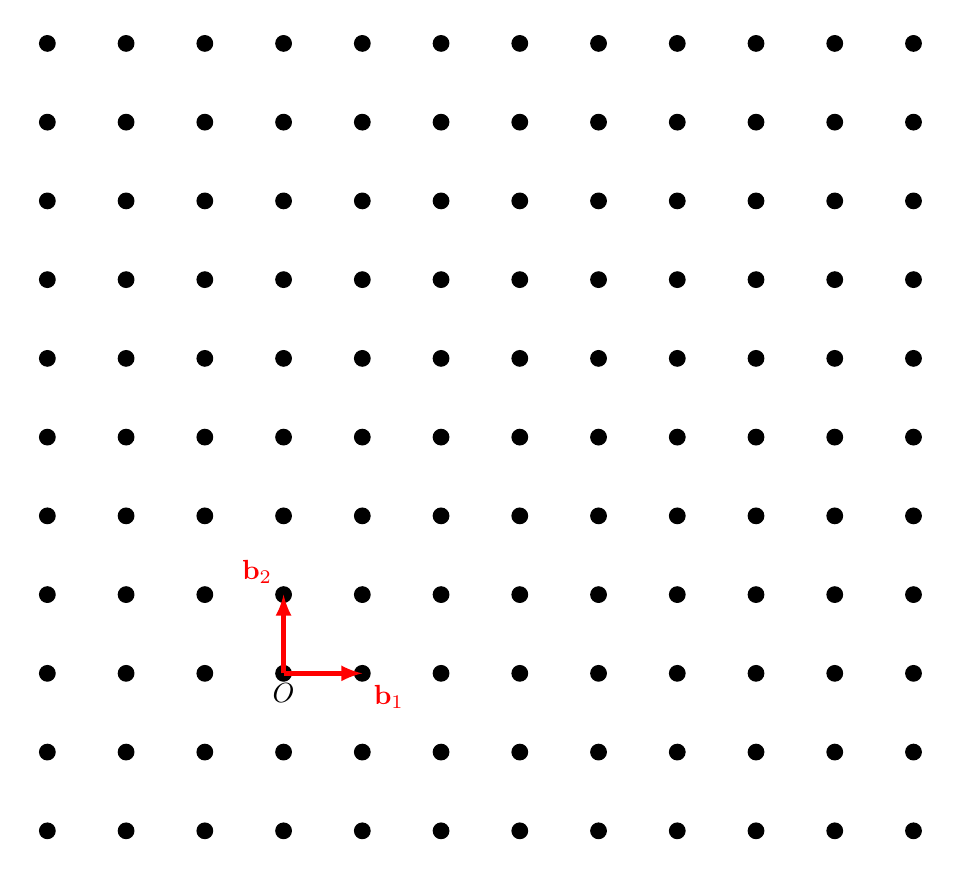
\begin{tikzpicture}
				\coordinate (Origin)  at (0,0);
				\node  at (0,0)  [below]{$O$};
				
				\clip (-3.25,-2.25) rectangle (8.2cm,8.2cm); % Clips the picture...
				\coordinate (Bone) at (0,1);
				\coordinate (Btwo) at (1,0);
				\foreach \x in {-10,-9,...,10}{% Two indices running over each
					\foreach \y in {-10,-9,...,10}{% node on the grid we have drawn 
						\node[draw,circle,inner sep=2pt,fill] at (\x,\y) {};
						\node[draw,circle,inner sep=1pt] at (\x,\y) {};
						% Places a dot at those points
					}
				}
				\draw [ultra thick,-latex,red] (Origin)
				-- (Bone) node [above left] {$\textbf{b}_2$};
				\draw [ultra thick,-latex,red] (Origin)
				-- (Btwo) node [below right] {$\textbf{b}_1$};
				
				
		\end{tikzpicture}}}
		\caption[A lattice]{The lattice formed from $\textbf{B} = \begin{pmatrix}1 & 0 \\ 0 & 1 \end{pmatrix}$} %$\textbf{B} = \begin{pmatrix}1 & 0 \\ 0 & 1 \end{pmatrix}$
		\label{fg:zn}
	\end{minipage}
	\begin{minipage}{.5\textwidth}
	\centering
	\framebox{
		\resizebox{.9\columnwidth}{.9\columnwidth}{%
	\begin{tikzpicture}
		\coordinate (Origin)  at (0,0);
		\node  at (0,0)  [below]{$O$};
		
		\clip (-3.25,-2.25) rectangle (8.2cm,8.2cm); % Clips the picture...
		\coordinate (Bone) at (1,2);
		\coordinate (Btwo) at (3,1);
		\foreach \x in {-10,-9,...,10}{% Two indices running over each
			\foreach \y in {-10,-9,...,10}{% node on the grid we have drawn 
				\node[draw,circle,inner sep=2pt,fill] at (\x+3*\y,2*\x+\y) {};
				\node[draw,circle,inner sep=1pt] at (\x,\y) {};
				% Places a dot at those points
			}
		}
		\draw [ultra thick,-latex,red] (Origin)
		-- (Bone) node [above left] {$\textbf{b}_1$};
		\draw [ultra thick,-latex,red] (Origin)
		-- (Btwo) node [below right] {$\textbf{b}_2$};
	

	\end{tikzpicture}}}
	\caption[A lattice]{The lattice formed from $\textbf{B} = \begin{pmatrix}1 & 3 \\ 2 & 1\end{pmatrix}$} %$
	\label{fg:b1-b2}
	\end{minipage}
\end{figure}
 
\paragraph{Fundamental parallelepiped} The \Define{fundamental parallelepiped} is the area bounded by all possible 0,1 combinations of the basis vectors, and is defined as the set of points $$\mathcal{P}(\textbf{B}) = \textbf{B}\cdot[0,1)^{n} = \left\{ \sum_{i=0}^{n} x_{i}\cdot\textbf{b}_{i}:\forall 0 \le x_{i} < 1 \right\}.$$
In Figure~\ref{fg:pb} you can see $\mathcal{P}(\textbf{B})$ highlighted.
If you think of the lattice as a wall, you can consider the fundamental parallelepiped as being a brick. The entire lattice is made up of an infinite amount of shifted copies of the fundamental parallelepiped, also known as a tiling. A visualisation of this can be seen in Figure~\ref{fg:tile}.
\\
The volume of a lattice, denoted $\mathtt{det}(\mathcal{L})$ is the defined as the volume of the fundamental parallelepiped, $\text{vol}(\mathcal{P}(\textbf{B}))$.
The volume of the fundamental parallelepiped is equal to the determinant of the basis:
$$\text{det}(\mathcal{L}(\textbf{B})) = \text{vol}(\mathcal{P}(\textbf{B})) = |\text{det}(\textbf{B})|. $$

\begin{figure}[ht]
	\begin{minipage}{.5\textwidth}
		\centering
		\framebox{
			\resizebox{.9\columnwidth}{.9\columnwidth}{%
				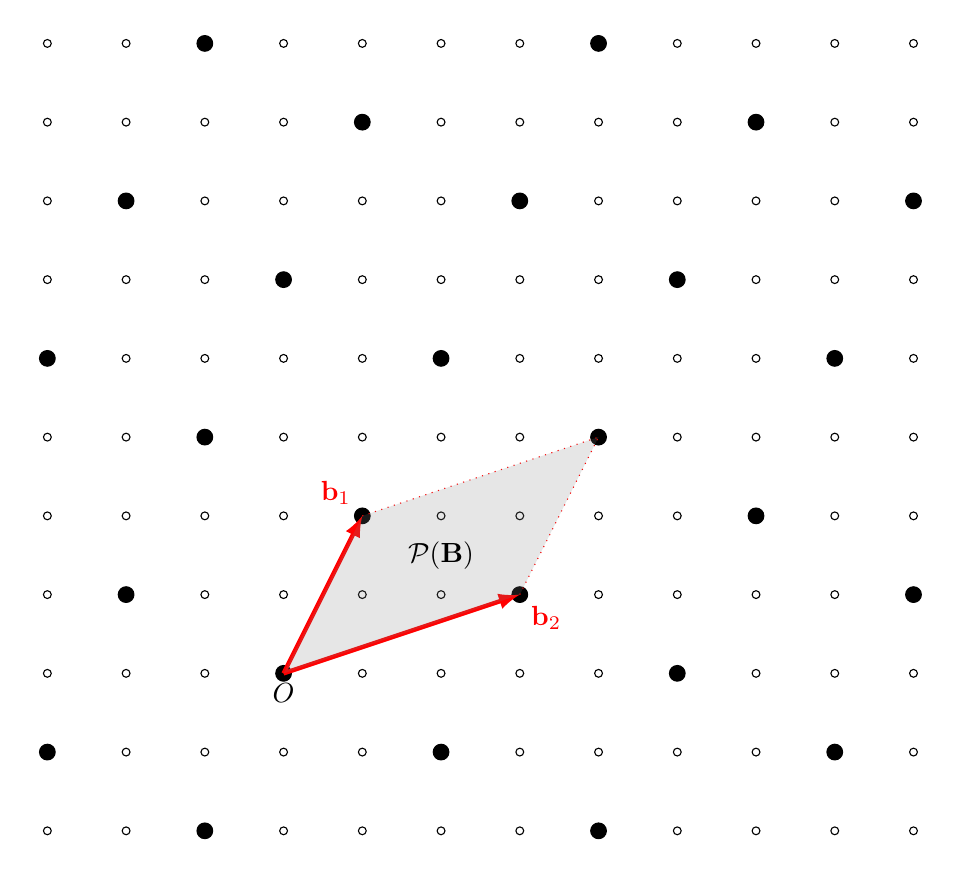
\begin{tikzpicture}
					\coordinate (Origin)  at (0,0);
					\node  at (0,0)  [below]{$O$};
					
					\clip (-3.25,-2.25) rectangle (8.2cm,8.2cm); % Clips the picture...
					\coordinate (Bone) at (1,2);
					\coordinate (Btwo) at (3,1);
					\coordinate (Bonetwo) at (4,3);
					\foreach \x in {-10,-9,...,10}{% Two indices running over each
						\foreach \y in {-10,-9,...,10}{% node on the grid we have drawn 
							\node[draw,circle,inner sep=2pt,fill] at (\x+3*\y,2*\x+\y) {};
							\node[draw,circle,inner sep=1pt] at (\x,\y) {};
							% Places a dot at those points
						}
					}
					\draw [ultra thick,-latex,red] (Origin)
					-- (Bone) node [above left] {$\textbf{b}_1$};
					\draw [ultra thick,-latex,red] (Origin)
					-- (Btwo) node [below right] {$\textbf{b}_2$};
					\draw [dotted,red] (Bone)
					-- (Bonetwo) node {};
					\draw [dotted,red] (Btwo)
					-- (Bonetwo) node {};
					\fill[gray,opacity=0.2] (Origin) -- (Bone) -- (Bonetwo) -- (Btwo) -- (Origin);
					
					\node at (2,1.5) {$\mathcal{P}(\textbf{B})$};
					
		\end{tikzpicture}}}
		\caption{The fundamental parallelepiped $\mathcal{P}(\textbf{B})$}
		\label{fg:pb}
	\end{minipage}
	\begin{minipage}{.5\textwidth}
	\centering
	\framebox{
		\resizebox{.9\columnwidth}{.9\columnwidth}{%
			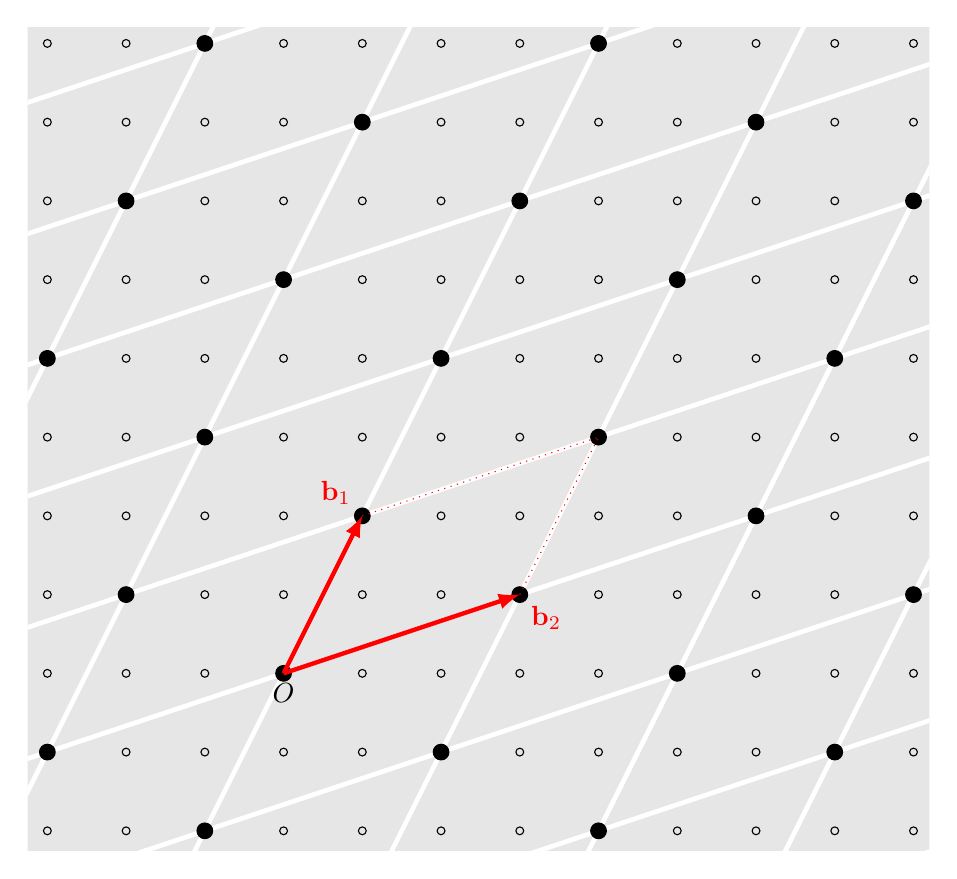
\begin{tikzpicture}

			 \clip (-3.25,-2.25) rectangle (8.2cm,8.2cm); % Clips the picture...	
				%\fill[gray,opacity=0.2] (Origin) -- (Bone) -- (Bonetwo) -- (Btwo) -- (Origin);
				\foreach \x in {-10,-9,...,10}{% Two indices running over each
					\foreach \y in {-10,-9,...,10}{% node on the grid we have drawn 
						%\vara = \x+3*\y
						%\varb = 2*\x+\y
						\fill[gray,opacity=0.2] (0+\x+3*\y,0+2*\x+\y) -- (1 + \x+3*\y,2+2*\x+\y) -- (4 +\x+3*\y,3+2*\x+\y) -- (3 +\x+3*\y,1+2*\x+\y) -- (0+\x+3*\y,0+2*\x+\y);
					}
				}
			  \foreach \x in {-10,-9,...,10}{% Two indices running over each
					  	\foreach \y in {-10,-9,...,10}{% node on the grid we have drawn 
					  		%\vara = \x+3*\y
					  		%\varb = 2*\x+\y
					  		\draw[ultra thick,white] (0+\x+3*\y,0+2*\x+\y) -- (1 + \x+3*\y,2+2*\x+\y) -- (4 +\x+3*\y,3+2*\x+\y) -- (3 +\x+3*\y,1+2*\x+\y) -- (0+\x+3*\y,0+2*\x+\y);
					  	}
			  	}
		  				\coordinate (Origin)  at (0,0);
		  \node  at (0,0)  [below]{$O$};
		  
		 
		  \coordinate (Bone) at (1,2);
		  \coordinate (Btwo) at (3,1);
		  \coordinate (Bonetwo) at (4,3);
		  \foreach \x in {-10,-9,...,10}{% Two indices running over each
		  	\foreach \y in {-10,-9,...,10}{% node on the grid we have drawn 
		  		\node[draw,circle,inner sep=2pt,fill] at (\x+3*\y,2*\x+\y) {};
		  		\node[draw,circle,inner sep=1pt] at (\x,\y) {};
		  		% Places a dot at those points
		  	}
		  }
		  \draw [ultra thick,-latex,red] (Origin)
		  -- (Bone) node [above left] {$\textbf{b}_1$};
		  \draw [ultra thick,-latex,red] (Origin)
		  -- (Btwo) node [below right] {$\textbf{b}_2$};
		  \draw [dotted,red] (Bone)
		  -- (Bonetwo) node {};
		  \draw [dotted,red] (Btwo)
		  -- (Bonetwo) node {};
				
				
	\end{tikzpicture}}}
	\caption{Tiling the lattice with $\mathcal{P}(\textbf{B})$}
	\label{fg:tile}
\end{minipage}
\end{figure}

\paragraph{Minimum distance} The \Define{minimum distance} ($\lambda_1$) on a lattice is the smallest distance between any two lattice points: $$\lambda_1 = \text{min}\{||\textbf{x} - \textbf{y}|| \forall \textbf{x},\textbf{y}\in\mathcal{L}, \textbf{x}\neq\textbf{y}\}.$$
The minimum distance of the lattice is also the length of the shortest vector in the lattice.
\\
Minkowski's theorem states that for any lattice, 
\[
    \lambda_1(\mathcal{L}) \leq \sqrt{n}\cdot\text{det}(\mathcal{L})^{1/n}. 
\]
This gives us an upper bound for the length of the shortest vector.
\subsection{Shortest Vector Problem} 
\Define{Shortest Vector Problem}.
\\
Instance: A lattice $\mathcal{L}(\textbf{B})$.
\\
Question: What is the shortest non-zero vector in the lattice? (i.e. find $\textbf{v} \in \mathcal{L}$ s.t. $||\textbf{v}|| = \lambda_1(\mathcal{L})$).
\\
~\\
There also exists an approximate version of this problem, where we are asked to find a vector that is at most $\gamma$ times the size of the longest vector. Where $\gamma = \gamma(n) \geq 1$.
\\
\Define{Approximate-Shortest Vector Problem}.
\\
Instance: A lattice $\mathcal{L}(\textbf{B})$.
\\
Question: Find a non-zero vector in the lattice that is at most $\gamma$ times longer than the shortest vector. (i.e. find $\textbf{v} \in \mathcal{L}$ s.t. $||\textbf{v}|| \leq \gamma(n)\cdot\lambda_1(\mathcal{L})$).
\\
~\\
SVP has been shown to be NP-Hard, for approximate-SVP the hardness depends on the approximation factor ($\gamma$). For $\gamma = O(1)$, approximate-SVP is "hard", for $\gamma = O(\sqrt{n})$ it's in NP $\cap$ co-NP, for $\gamma = 2^{\tilde{O}(n)}$ it's in P. For crypto we tend to rely on the hardness of approximate-SVP for $\gamma$ = poly($n$).
\\
There are a number of approaches for solving SVP, we'll discuss two of them.
\paragraph{Enumeration} The `brute force' method of solving SVP is enumeration, given a lattice we enumerate through every lattice point in some bounded region, typically the fundamental parallelepiped. Whilst very slow, this method is still often used as it has very low memory requirements.
\paragraph{Sieving} Sieving algorithms are randomised algorithms that, in some cases, run very efficiently but use an exponential amount of space. They work by generating some random lattice points and then taking the difference between these points (Figure~\ref{fg:sieve1}). The difference between any two lattice points is also a valid lattice point, and so this is then added to the list (Figure~\ref{fg:sieve2}). Hopefully as this is repeated a short vector is found.

\begin{figure}[ht]
	\begin{minipage}{.5\textwidth}
		\centering
		\framebox{
			\resizebox{.9\columnwidth}{.9\columnwidth}{%
				\begin{tikzpicture}
					\coordinate (Origin)  at (0,0);
					\node  at (0,0)  [below]{\Huge O};
					
					%\clip (-30,-30) rectangle (40,40); % Clips the picture...
					\coordinate (Bone) at (1,2);
					\coordinate (Btwo) at (3,1);
					\coordinate (Bonetwo) at (4,3);
					\foreach \x in {-30,-29,...,30}{% Two indices running over each
						\foreach \y in {-30,-29,...,30}{% node on the grid we have drawn 
							\pgfmathparse{\x+3*\y}
							\ifnum -20 < \pgfmathresult 
								\pgfmathparse{\x+3*\y}
								\ifnum  20 > \pgfmathresult 
								\pgfmathparse{2*\x+\y}
								\ifnum -20 < \pgfmathresult 
								\pgfmathparse{2*\x+\y}
								\ifnum 20 > \pgfmathresult 
							%\ifthenelse{-5 < (\x+3*\y) \AND (\x+3*\y< 5) \AND -5 < 2*\x+\y \AND 2*\x+\y<5}{
									\node[draw,circle,inner sep=2pt,fill,black] at (\x+3*\y,2*\x+\y) {};
								\fi
							\fi
							\fi
							\fi
							%\node[draw,circle,inner sep=1pt] at (\x,\y) {};
							% Places a dot at those points
						}
					}
					\coordinate (r1) at (9,-2);
					\coordinate (r2) at (-18,-6);
					\coordinate (r3) at (7,4); 
					\coordinate (r4) at (6,12); 
					\coordinate (r5) at (-6,-2); 
					\coordinate (r6) at (10,10); 
					\coordinate (r7) at (-6,-12);
					\coordinate (r8) at (-6,8);
					\coordinate (r9) at (-16,-12);
					\coordinate (r10) at (12,-6);
					
					\node[draw,circle,inner sep=5pt,fill,red] at (Origin) {};
					  			
					\node[draw,circle,inner sep=5pt,fill,red] at (r1) {};
					\node[draw,circle,inner sep=5pt,fill,red] at (r2) {};
					\node[draw,circle,inner sep=5pt,fill,red] at (r3) {};
					\node[draw,circle,inner sep=5pt,fill,red] at (r4) {};
					\node[draw,circle,inner sep=5pt,fill,red] at (r5) {};
					\node[draw,circle,inner sep=5pt,fill,red] at (r6) {};
					\node[draw,circle,inner sep=5pt,fill,red] at (r7) {};
					\node[draw,circle,inner sep=5pt,fill,red] at (r8) {};
					\node[draw,circle,inner sep=5pt,fill,red] at (r9) {};
					\node[draw,circle,inner sep=5pt,fill,red] at (r10) {};
					
				\draw [ultra thick,-latex,black] (r4)
				-- (r6);
				
				\draw [ultra thick,-latex,black] (r1)
				-- (r10);
				
				\draw [ultra thick,-latex,black] (r2)
				-- (r9);
					
	\end{tikzpicture}}}
		\caption{Choosing some random points and finding the differences.}
		\label{fg:sieve1}
	\end{minipage}
	\begin{minipage}{.5\textwidth}
		\centering
		\framebox{
			\resizebox{.9\columnwidth}{.9\columnwidth}{%
				\begin{tikzpicture}
					\coordinate (Origin)  at (0,0);
					\node  at (0,0)  [below]{\Huge O};
					
					%\clip (-30,-30) rectangle (40,40); % Clips the picture...
					\coordinate (Bone) at (1,2);
					\coordinate (Btwo) at (3,1);
					\coordinate (Bonetwo) at (4,3);
					\foreach \x in {-30,-29,...,30}{% Two indices running over each
						\foreach \y in {-30,-29,...,30}{% node on the grid we have drawn 
							\pgfmathparse{\x+3*\y}
							\ifnum -20 < \pgfmathresult 
							\pgfmathparse{\x+3*\y}
							\ifnum  20 > \pgfmathresult 
							\pgfmathparse{2*\x+\y}
							\ifnum -20 < \pgfmathresult 
							\pgfmathparse{2*\x+\y}
							\ifnum 20 > \pgfmathresult 
							%\ifthenelse{-5 < (\x+3*\y) \AND (\x+3*\y< 5) \AND -5 < 2*\x+\y \AND 2*\x+\y<5}{
							\node[draw,circle,inner sep=2pt,fill,black] at (\x+3*\y,2*\x+\y) {};
							\fi
							\fi
							\fi
							\fi
							%\node[draw,circle,inner sep=1pt] at (\x,\y) {};
							% Places a dot at those points
						}
					}
					\coordinate (r1) at (9,-2);
					\coordinate (r2) at (-18,-6);
					\coordinate (r3) at (7,4); 
					\coordinate (r4) at (6,12); 
					\coordinate (r5) at (-6,-2); 
					\coordinate (r6) at (10,10); 
					\coordinate (r7) at (-6,-12);
					\coordinate (r8) at (-6,8);
					\coordinate (r9) at (-16,-12);
					\coordinate (r10) at (12,-6);
					
					\node[draw,circle,inner sep=5pt,fill,red] at (Origin) {};
					
					\node[draw,circle,inner sep=5pt,fill,red] at (r1) {};
					\node[draw,circle,inner sep=5pt,fill,red] at (r2) {};
					\node[draw,circle,inner sep=5pt,fill,red] at (r3) {};
					\node[draw,circle,inner sep=5pt,fill,red] at (r4) {};
					\node[draw,circle,inner sep=5pt,fill,red] at (r5) {};
					\node[draw,circle,inner sep=5pt,fill,red] at (r6) {};
					\node[draw,circle,inner sep=5pt,fill,red] at (r7) {};
					\node[draw,circle,inner sep=5pt,fill,red] at (r8) {};
					\node[draw,circle,inner sep=5pt,fill,red] at (r9) {};
					\node[draw,circle,inner sep=5pt,fill,red] at (r10) {};
					
					\draw [ultra thick,-latex,black] (r4)
					-- (r6);
					
					\draw [ultra thick,-latex,black] (r1)
					-- (r10);
					
					\draw [ultra thick,-latex,black] (r2)
					-- (r9);
					
					\coordinate (n1) at (4,-2);
					\coordinate (n2) at (3,-4);
					\coordinate (n3) at (-2,6);
					
					\node[draw,circle,inner sep=5pt,fill,blue] at (n1) {};
					\node[draw,circle,inner sep=5pt,fill,blue] at (n2) {};
					\node[draw,circle,inner sep=5pt,fill,blue] at (n3) {};
					
					\draw [ultra thick,-latex,black] (n1)
					-- (Origin);
					
					\draw [ultra thick,-latex,black] (n2)
					-- (Origin);
					
					\draw [ultra thick,-latex,black] (n3)
					-- (Origin);
					
		\end{tikzpicture}}}
		\caption{Adding the new vectors to the list, ready to repeat.}
		\label{fg:sieve2}
	\end{minipage}
\end{figure}

\subsection{Breaking LWE}
The main method for breaking LWE involves turning it into a SVP instance. Given an LWE instance $(\textbf{A},\textbf{b}),~ \textbf{b} = \textbf{A}\cdot\textbf{s} + \textbf{e}$, we can construct an SVP instance by creating a lattice basis $$\textbf{B} = \begin{pmatrix}
	\textbf{A}^{\top} & 0 \\
	\textbf{b}^{\top} & 1 
\end{pmatrix} \in \mathbb{Z}^{(n+1)\times(m+1)}_{q}.$$ Every point on this lattice can be defined by $\begin{pmatrix}\textbf{x}^{\top}|y\end{pmatrix}\cdot\textbf{B} = \begin{pmatrix}\textbf{x}^\top\cdot\textbf{A}^{\top} + y\cdot\textbf{b}^{\top}\\ y\end{pmatrix}$, where $\textbf{x} \in \mathbb{Z}^{n}$ and $y\in\mathbb{Z}$.
The length of the vector represented by this point is minimised when $\textbf{x}^\top\cdot\textbf{A}^{\top} + y\cdot\textbf{b}^{\top}$ is at its minimum, in fact the length of this vector is at its shortest when $\textbf{x} = \textbf{s}$ and $y = -1$, giving us $\begin{pmatrix}\textbf{s}^{\top}\cdot\textbf{A}^{\top} -\textbf{b}^{\top}|-1\end{pmatrix} = \begin{pmatrix}(\textbf{A}\cdot\textbf{s}-\textbf{b})^\top|-1\end{pmatrix}= \begin{pmatrix}\textbf{e}^\top|-1\end{pmatrix}$.
\\
If we can find the shortest vector in this lattice $\begin{pmatrix}\textbf{e}^\top|-1\end{pmatrix}$, then we can calculate $\begin{pmatrix}\textbf{e}^\top|-1\end{pmatrix}\cdot\textbf{B}^{-1} =\begin{pmatrix}\textbf{s}^\top|-1\end{pmatrix}$ and therefore have solved the LWE instance.
\subsection{See further}
\paragraph{Homomorphic encryption} LWE is very versatile, and has opened up new branches of cryptography. It has allowed cryptographers to create the first homomorphic encryption system, where the exists some addition (or multiplication) such that applying that function to two ciphertexts and decrypting would give the same result as just adding (or multiplying) the initial plaintexts, i.e. $d(Add(e(p1),e(p2))) = p1 + p2$, where $e(),~d()$ are the encryption and decryption functions. 

\paragraph{What other crypto is there?} Cryptography is an ever expanding field of research, other interesting areas include:
\begin{itemize}
	\item Multi-party computation - multiple users want to perform a computation on all their inputs, without anyone revealing their inputs.
	\item Threshold cryptography - a group of $n$ users want to encrypt some data, such that for some $t<n$, any subgroup of these users of size at least $t$ can decrypt the data while any subgroup of these users of size less than $t$ are unable to.
	\item Zero knowledge proofs - prove to someone that you know some value without giving away the value.
	\item Random number generation.
\end{itemize}




\chapter{Error-correcting codes}


\section{Linear codes I: Introduction to error-correcting codes}
\label{sec:21}



\subsection{Error control}

\paragraph{The tenets of error control}
Messages are subject to errors when transmitted through a channel. The channel can either be spatial (data transmission) or temporal (storage).
%\begin{figure}
%\begin{center}
%\includegraphics[scale=0.15]{system.jpg}
%\end{center} \caption{Digital communication system}
%\end{figure}
The main advantage of digital data over analog data is that  we can perform error correction. We use two main assumptions:
\begin{itemize}
	\item We simplify the channel.
	
	\item We suppose errors occur infrequently.
\end{itemize}
The main idea is to \Important{add redundancy} to the data.


\paragraph{The codebook idea}
The language itself is an error correcting code:
\begin{quote}
    ``I am going to the con\Important{k}ert tonight.''\\ 
\end{quote}
In this case, it is easy to detect and correct the error:
\begin{quote}
    ``I am going to the concert tonight.''
\end{quote}
Some sequences of letters are correct, others are incorrect. The correct ones form a \Important{code}.


\subsection{Binary repetition and parity-check codes}

\paragraph{Basic error detection}
Binary \Define{parity-check code}: add one more bit to the sequence of bits so that the overall number of 1's is even. For instance,
\[
    1100011 \xrightarrow{\text{encoding}} 1100011\Structure{0}
\]
The codebook then consists of all sequences of a given length with an even number of bits equal to $1$. This was used in the first version of ASCII (7 bits for the symbol + 1 parity-check bit).


%\paragraph{ASCII table}
%\begin{figure}
%\includegraphics[scale=0.6]{asciifull.jpg}
%\end{figure}
%

The parity-check code can \Important{detect one error} (simply check the number of ones!) e.g. 
\[
	1100011 \xrightarrow{\text{encoding}} 11000110 \xrightarrow{\text{channel}} 110\Structure{1}0110
\]
It cannot detect two errors: 
\[
	1100011 \xrightarrow{\text{encoding}} 11000110 \xrightarrow{\text{channel}} 110\Structure{11}110
\]
It \Important{cannot correct any error}: e.g. if we receive $11010110$, what happened?
\begin{align*}
	1100011 \xrightarrow{\text{encoding}} 11000110 &\xrightarrow{\text{channel}} 110\Important{1}0110 \quad or \\
	1101011 \xrightarrow{\text{encoding}} 11010111 &\xrightarrow{\text{channel}} 1101011\Important{0} \quad ?
\end{align*}
In this case, there are eight possible scenarios, one for each error location.


\paragraph{Basic error correction}
Binary \Define{repetition code}: send the same bit $n$ times (e.g. $n=3$)
\begin{align*}
	0 &\to 000\\
	1 &\to 111.
\end{align*}
The codebook consists of two codewords: $\{000,111\}$.

The repetition code can \Important{correct $\lfloor \frac{n-1}{2} \rfloor$ errors} e.g. 
\begin{align*}
	0 &\xrightarrow{\text{encoder}} 000 \xrightarrow{\text{channel}} 0\Structure{1}0 \xrightarrow{\text{decoder}} 0\\
	1 &\xrightarrow{\text{encoder}} 111 \xrightarrow{\text{channel}} 11\Structure{0} \xrightarrow{\text{decoder}} 1
\end{align*}
It can detect $n-1$ errors e.g. $0 \to 000 \to \Structure{11}0$. However, the repetition code has a very low rate: $\frac{1}{n}$! We need more rate-efficient techniques.



\paragraph{Objectives}
We want to design a ``good'' error correcting code, i.e.
\begin{enumerate}
	\item Detects and corrects many errors
	\item High rate
	\item Easy to encode and decode.
\end{enumerate}
The first two are conflicting: compromise depending on the channel quality. We will mainly focus on \Important{error correction} over detection.


\subsection{Minimum distance}

\paragraph{Hamming distance}
The \Define{Hamming distance} between two vectors is the number of times they disagree. E.g. $\dH(100,101) = 1$. It is a metric:
\begin{enumerate}
	\item $\dH({\bf x},{\bf y}) \ge 0$,
	\item $\dH({\bf x},{\bf y}) = \dH({\bf y},{\bf x})$,
	\item $\dH({\bf x},{\bf y}) = 0$ if and only if ${\bf x}={\bf y}$,
	\item $\dH({\bf x},{\bf y}) \le \dH({\bf x},{\bf z}) + \dH({\bf z},{\bf y})$ (triangular inequality).
\end{enumerate}
Thus, it has a \Important{geometric} meaning.

The \Define{Hamming weight} of a vector is simply the number of nonzero coefficients:
\[
	\wH({\bf x}) = \dH({\bf x}, {\bf 0}).
\]


\paragraph{Hamming distance and error correction}
The \Important{decoding} problem is as follows. If the destination receives the vector ${\bf v}$, the decoder returns the unique nearest (in terms of Hamming distance) codeword to ${\bf v}$ if it exists.

Problem: what if that codeword is not unique? We thus need a sufficient condition to make sure the decoding is non-ambiguous.


\paragraph{Minimum distance}
A \Define{code} $\code{C}$ is a subset of $[q]^n$, where $[q]$ represents any set of size $q$. The \Define{minimum distance} of $\code{C}$, denoted $\dmin(\code{C})$, is the minimum Hamming distance between two distinct codewords in $\code{C}$:
\[
    \dmin(\code{C}) := \min\{ \dH({\bf c}, {\bf c}'): {\bf c}, {\bf c}' \in \code{C}, {\bf c} \ne {\bf c}' \}. 
\]

\begin{theorem}
A code can correct $t$ errors if and only if it has minimum distance $\dmin \ge 2t+1$.
\end{theorem}

\begin{proof}
For any ${\bf c} \in \GF(q)^n$, let $S_r({\bf c})$ denote the \Define{sphere} of Hamming radius $r$ centred around ${\bf c}$:
\[
    S_r({\bf c}) = \left\{ {\bf v} \in \GF(q)^n : \dH({\bf v}, {\bf c}) \le r  \right\}.
\]
Then it is clear that $\code{C}$ corrects $t$ errors if and only if $S_t({\bf c}) \cap S_t({\bf c}') = \emptyset$ for distinct codewords ${\bf c}$ and ${\bf c}'$.

Suppose $S_t({\bf c}) \cap S_t({\bf c}') \ne \emptyset$ for distinct codewords ${\bf c}$ and ${\bf c}'$, say $\dH({\bf v}, {\bf c}) \le t$ and $\dH({\bf v}, {\bf c}') \le t$. Then the triangular inequality yields
\[
    \dH({\bf c}, {\bf c}') \le \dH({\bf v}, {\bf c}) + \dH({\bf v}, {\bf c}') \le 2t,
\]
and hence $\dmin \le 2t$.

Conversely, let $\code{C}$ have minimum distance $\dmin \le 2t$. Let ${\bf c}, {\bf c}' \in \code{C}$ at Hamming distance $2t$; we now construct ${\bf v} \in S_t({\bf c}) \cap S_t({\bf c}')$. This is clear if $\dmin \le t$, so we assume $\dmin > t$. Let $\Delta$ be the set of coordinates where ${\bf c}$ and ${\bf c}'$ disagree, i.e. $|\Delta| \le 2t$ and ${\bf c}_j \ne {\bf c}_j$ for all $j \in \Delta$. Select $\Gamma \subseteq \Delta$ with $|\Gamma| = t$, and define
\[
    {\bf v}_\Gamma = {\bf c}_\Gamma, \qquad
    {\bf v}_{\Delta \setminus \Gamma} = {\bf c}'_{\Delta \setminus \Gamma}, \qquad
    {\bf v}_{\{1, \dots, n\} \setminus \Delta} = {\bf c}_{\{1, \dots, n\} \setminus \Delta} = {\bf c}'_{\{1, \dots, n\} \setminus \Delta}.
\]
Then indeed $\dH({\bf v}, {\bf c}) = \dmin  - t \le t$ and $\dH({\bf v}, {\bf c}') = t$.
\end{proof}


\subsection{Bounds on codes}


Let $A(n,q,d)$ be the maximum cardinality of a $q$-ary code of length $n$ and minimum distance (at least) $d$. 
The volume $|S_r({\bf c})|$ of the sphere does not depend on its centre and is denoted by 
$V(n,q,r)$.

\paragraph{Sphere-packing bound}
The \Important{sphere-packing bound} (a.k.a. Hamming bound) is an upper bound on $A(q,n,d)$.


\begin{theorem}[Sphere-packing bound.]
\[
	A(n,q,d) \le \frac{ q^n }{ V \left( n,q, \left\lfloor \frac{d-1}{2} \right\rfloor \right) } .
\]
\end{theorem}

\begin{proof}
Let $\code{C}$ be an optimal code with cardinality $A(n,q,d)$. Let $t = \left\lfloor \frac{d-1}{2} \right\rfloor$. The spheres of radius $t$ centred around the codewords do not overlap (they are the decoding regions!) and hence can be \Important{packed}. Thus there are $|\code{C}| V(n,q,t) \le q^n$ vectors in those spheres.
\end{proof}

\paragraph{Gilbert bound}
The \Important{Gilbert bound} (a.k.a. Gilbert-Varshamov bound) is a lower bound on $A(q,n,d)$. From the proof one can easily derive a greedy algorithm to produce a code whose cardinailty reaches or surpasses that bound.

\begin{theorem}[Gilbert bound]
\[
	A(n,q,d) \ge \frac{ q^n }{ V(n, q, d-1 ) }.
\]
\end{theorem}

\begin{proof}
Let $\code{C}$ be an optimal code with cardinality $A(n,q,d)$. For every vector ${\bf v} \in \GF(q)^n$, there exists ${\bf c} \in \code{C}$ at Hamming distance at most $d-1$, for otherwise $\code{C} \cup \{ {\bf v} \}$ would have minimum distance $\ge d$ and a larger cardinality. In other words, the spheres of radius $d-1$ centred around the codewords \Important{cover} the whole space. There are $q^n \le |\code{C}| V(n,q,d-1)$ vectors.
\end{proof}


\subsection{See further}

\paragraph{Other metrics}
In this course, we will focus on traditional error-correcting codes, where the codewords are vectors and the distance between two codewords is the Hamming distance. However, other metrics have been proposed for different situations. We mention two below.

Firstly, the Hamming metric does not take into account the amplitude of an error: if a coordinate is changed during transmission, then it yields one Hamming error, whatever it is. On the other hand, the \Important{Lee metric} has been proposed for situations where the amplitude matters, such as phase modulated signals (and again, errors with low amplitude are less likely than errors with high magnitude). Formally, let $[q] = \{0, 1, \dots, q-1\}$, and for any $a,b \in [q]$ let
\[
    l(a,b) = \min\{ |a - b|, q - |a - b| \}
\]
(imagine the symbols being placed on a cycle you can turn clockwise or anticlockwise). Then the Lee distance between ${\bf x}$ and ${\bf y}$ is simply $\sum_i l(x_i,y_i)$.

Secondly, consider data that is stored in a two-dimensional array (like your campus card). Typical errors may corrupt a whole (or at least a significant part of a) column or row of that array. The \Important{rank metric} was proposed for that scenario. The codewords are $m \times n$ matrices, and the distance between two matrices ${\bf M}$ and ${\bf N}$ is the rank distance $\mathrm{rank}({\bf M} - {\bf N})$. Note that corrupting a whole row corresponds to adding a matrix ${\bf E}$ where the nonzero entries are confined to that row (and hence $\mathrm{rank}({\bf E}) = 1$). The same holds for columns. Therefore, corrupting $t$ rows or columns amounts to adding a matrix ${\bf E}_t$ with $\mathrm{rank}({\bf E}_t) \le t$.

\paragraph{Other bounds on codes}
Many more bounds on codes have been derived. We can briefly mention the Singleton bound, the Plotkin bound, the Johnson bound, the code-anticode bound, linear programming bounds, etc.


\paragraph{The EAN}
The \Define{International Article Number} (underneath the barcode) uses a variant of the parity-check code: ${\bf c} = (c_1,\ldots,c_{13})$, where
\[
	c_{13} = -\sum_{i=0}^5 (c_{2i+1} + 3c_{2i+2}) \mod 10.
\]
For instance, let us determine the last symbol of this barcode: $5-045092-36551\Important{?}$
\begin{align*}
	c_{13} &= -\left[5 + (3 \times 0) + 4 + (3 \times 5) + 0 + (3 \times 9) + 2 + (3 \times 3) + 6 + (3 \times 5) + 5 + (3 \times 1)  \right] \mod 10\\
	&= -1 \mod 10\\
	&= 9.
\end{align*}

% \paragraph{ISBN-10}
% The \Define{ISBN-10} code: Another variant of the parity-check code 
% \[
% 	c_{10} = \sum_{i=1}^9 i c_i \mod 11.
% \]
% (The letter $X$ is used for $10$.) Two most common errors in handling an ISBN:
% \begin{itemize}
% 	\item An altered digit

% 	\item The transposition of adjacent digits
% \end{itemize}
% The ISBN-10 code detects one of these two errors.

% For example: ISBN-10 number $0-262-06141-\Important{?}$
% \begin{align*}
% 		c_{10} &= \big[ (1 \times 0) + (2 \times 2) + (3 \times 6) + (4 \times 2) + (5 \times 0)\\
% 		& + (6 \times 6) + (7 \times 1) + (8 \times 4) + (9 \times 1) \big]\\
% 		&= 4 + 7 + 8+3+7+10+9\\
% 		&=4.
% \end{align*}
% The new ISBN-13 (2005) uses the International Article Number instead.



\subsection{Exercises}



\begin{exercise}
Prove that the Hamming distance is a metric on $[q]^n$.
\end{exercise}




\begin{exercise}
Prove that if ${\bf x}, {\bf y} \in \{0,1\}^n$ have the same Hamming weight, then their Hamming distance is even.
\end{exercise}






% \begin{exercise}
% Let ${\bf c} \in [q]^n$ and consider the ball of radius $r$ around ${\bf c}$: $B_r({\bf c}) = \{ {\bf v} \in [q]^n : \dH( {\bf c} , {\bf v} ) \le r  \}$. Prove that
% \[
% 	|B_r({\bf c})| = \sum_{d=0}^r \binom{n}{d} (q-1)^d;
% \]
% which is denoted as $V(q,n,r)$ in the lecture slides.
% \end{exercise}





\begin{exercise}
Prove that 
\[
    V(q,n,r) = \sum_{d=0}^r \binom{n}{d} (q-1)^d.
\]
\end{exercise}


\begin{exercise}
Prove that for any ${\bf x}, {\bf y} \in [q]^n$ at distance $d$, and any $0 \le t \le d$, there are exactly $\binom{d}{t}$ vectors ${\bf v} \in [q]^n$ such that $\dH({\bf v}, {\bf x}) = t$ and $\dH({\bf v}, {\bf y}) = d-t$.
\end{exercise}


\begin{exercise}
Find out how the CIS id's (e.g. ``bcdf12'') are generated. I suspect at least one of the two digits is some form of parity-check, but I don't know!
\end{exercise}










\section{Linear codes II: Finite fields}
\label{sec:22}



\subsection{Construction of finite fields}

\paragraph{Finite fields}
A \Define{field} is an algebraic structure in which we can add, subtract, multiply and divide (and multiplication distributes over addition), just like over the real numbers.


More formally, a group is a pair $(G, \cdot)$ where $G$ is a set and $\cdot$ is binary operation on $G$ that satisfies the three following properties (for all $a,b,c \in G$):
\begin{enumerate}
    \item Associativity: $a \cdot (b \cdot c) = (a \cdot b) \cdot c$.
    
    \item Identity element: there exists $e \in G$ such that $a \cdot e = e \cdot a = a$.
    
    \item Inverses: there exists $a^{-1}$ such that $a \cdot a^{-1} = a^{-1} \cdot a = e$.
\end{enumerate}
If furthermore, the operation is commutative, i.e. $a \cdot b = b \cdot a$, then the group $(G, \cdot)$ is called abelian. A field is a $5$-tuple $(F, +, \times, 0, 1)$ such that
\begin{enumerate}
    \item $(F, +)$ is an abelian group with identity $0$.
    
    \item $(F^*, \times)$ is an abelian group with identity $1$.
    
    \item Multiplication distributes over addition: $a \times (b + c) = (a \times b) + (a \times c)$.
\end{enumerate}
For instance, $(\R, +, \times, 0, 1)$ is a field. We use similar notation for any other field $F$ e.g. writing $-a$ for the additive inverse of $a$.


\begin{theorem}[Galois] Any finite field is of order (size) $q = p^m$, where $p$ is a prime number and $m$ is any integer $\ge 1$. Moreover, all fields of size $q$ are the same (up to renaming elements).
\end{theorem}

We can then talk about the field of order $q$, commonly denoted as $\GF(q)$ or $\mathbb{F}_q$.



\paragraph{Prime fields $\GF(p)$} 
Finite fields of prime order $\GF(p)$ are simply modular arithmetic $\mod p$. E.g. $p=5$\\
~\\
\begin{tabular}{c|ccccc}
	+ & 0 & 1 & 2 & 3 & 4\\
	\hline
	0 & 0 & 1 & 2 & 3 & 4\\
	1 & 1 & 2 & 3 & 4 & 0\\
	2 & 2 & 3 & 4 & 0 & 1\\
	3 & 3 & 4 & 0 & 1 & 2\\
	4 & 4 & 0 & 1 & 2 & 3
\end{tabular} \hspace{2cm}
\begin{tabular}{c|ccccc}
	$\times$ & 0 & 1 & 2 & 3 & 4\\
	\hline
	0 & 0 & 0 & 0 & 0 & 0\\
	1 & 0 & 1 & 2 & 3 & 4\\
	2 & 0 & 2 & 4 & 1 & 3\\
	3 & 0 & 3 & 1 & 4 & 2\\
	4 & 0 & 4 & 3 & 2 & 1
\end{tabular}
~\\
~\\
We can indeed add, and subtract: $-1 = 4$, $-2 = 3$, $-3 = 2$, $-4 = 1$.\\
We can multiply and divide (not by zero, of course): $1^{-1} = 1$, $2^{-1} = 3$, $3^{-1} = 2$, $4^{-1} = 4$.

This holds for all prime $p$. The only nontrivial thing to prove is that every nonzero integer $\beta \in \Z_p^*$ has an inverse. This follows from a fundamental result about the gcd: if $a,b \in \Z$ have $\gcd(a,b) = d$, then there exist $s, t \in \Z$ such that $as + bt = d$. Since $\gcd(\beta, p) = 1$, there exists $\gamma$ such that $\beta \gamma = 1 \mod p$.


\paragraph{Extension fields $\GF(p^m)$}
The extension field $\GF(p^m)$ is constructed as follows. Let $P(x)$ be a polynomial of degree $m$ over $\GF(p)$. We say $P(x)$ is \Define{irreducible} if it cannot be factored as $P(x) = Q(x)R(x)$ with $\deg Q(x), \deg R(x) < m$. We say $P(x)$ is \Define{primitive} if it is irreducible and the smallest positive integer $n$ such that $P(x) \mid x^n - 1$ is $n = p^m-1$.

Now, choose a primitive polynomial $P(x)$ of degree $m$ over $\GF(p)$, and let $\alpha$ be a root. Then 
\[
    \GF(p^m) = \{ 0, 1, \alpha, \alpha^2, \dots, \alpha^{p-2} \}
\]



For example, let us construct $\GF(4)$. Let $\alpha$ be a root of $x^2 + x + 1$, i.e. 
\[
	\alpha^2 + \alpha + 1 = 0, \quad \mbox{or equivalently,} \quad \Structure{\alpha^2 = \alpha+1}.
\]


\begin{tabular}{c|c|c|c|c|}
	+ & 0 & 1 & $\alpha$ & $\alpha+1$\\
	\hline
	0 & 0 & 1 & $\alpha$ & $\alpha+1$\\
	\hline
	1 & 1 & 0 & $\alpha+1$ & $\alpha$\\
	\hline
	$\alpha$ & $\alpha$ & $\alpha+1$ & 0 & 1\\
	\hline
	$\alpha+1$ & $\alpha+1$ & $\alpha$ & 1 & 0\\
	\hline
\end{tabular}
\hfill
\begin{tabular}{c|c|c|c|c|}
	$\times$ & 0 & 1 & $\alpha$ & $\alpha^2$\\
	\hline
	0 & 0 & 0 & 0 & 0\\
	\hline
	1 & 0 & 1 & $\alpha$ & $\alpha^2$\\
	\hline
	$\alpha$ & 0 & $\alpha$ & $\alpha^2$ & 1\\
	\hline
	$\alpha^2$ & 0 & $\alpha^2$ & 1 & $\alpha$\\
	\hline
\end{tabular}
~\\
~\\
The field $\GF(8)$ can be constructed similarly. Let $\alpha$ be a root of $x^3 + x + 1$, i.e. 
\[
	\alpha^3 + \alpha + 1 = 0.
\]
Then 
\[
    \GF(8) = \{0,1,\alpha,\alpha^2,\alpha^3  = \alpha+1, \alpha^4 = \alpha^2 + \alpha, \alpha^5 = \alpha^2 + \alpha + 1, \alpha^6 = \alpha^2 + 1\}.
\]


\subsection{Properties}

\paragraph{Multiplicative structure}
The multiplicative structure of $\GF(q)^*$ is very simple: it is that of a cyclic group of order $q-1$. More concretely, 
\[
    \GF(q)^* = \{\alpha, \alpha^2, \dots, \alpha^{q-2}, \alpha^{q-1} = 1\},
\]
where $\alpha$ is the root of $P(x)$. This is the \Important{exponential notation}. Let $\beta \in \GF(q)^*$, then $\beta = \alpha^k$ for some $0 \le k \le q-2$, thus
\[
    \beta^{q-1} = \left( \alpha^k \right)^{q-1} = \left( \alpha^{q-1} \right)^k = 1.
\]
For any $\beta \in GF(q)^*$, the \Define{order} of $\beta$, denoted as $o(\beta)$ is the smallest positive integer $t$ such that $\beta^t = 1$. If $o(\beta) = q-1$, then $\beta$ is said to be \Define{primitive} (and hence any element in $\GF(q)^*$ can be expressed as a power of $\beta$).



\paragraph{Additive structure}
For any $\beta \in \GF(p^m)$, we have
\[
	p \beta = \underbrace{\beta + \beta + \dots + \beta}_{p \text{ times}} = 0.
\]
We say that $p$ is the \Define{characteristic} of $\GF(p^m)$. Consequently, for any $\beta, \gamma \in \GF(p^m)$, 
\[
	(\beta + \gamma)^p = \beta^p + \gamma^p.
\]

$\GF(p^m)$ forms a vector space of dimension $m$ over $\GF(p)$, with the \Define{polynomial basis} $(1, \alpha, \dots, \alpha^{m-1})$.
This yields the \Important{polynomial notation}:
\[
	\beta = \sum_{i=0}^{m-1} \beta_i \alpha^i \quad \beta_i \in \GF(p).
\]


\paragraph{Subfields}
In general, we can construct $\GF(q^m)$ from a primitive polynomial over $\GF(q)$. Then $\GF(q^m)$ contains $\GF(q^n)$ as a subfield if and only if $n \mid m$. For instance, $\GF(64) = \GF(2^6)$ contains $\GF(2^6)$, $\GF(2^3)$, $\GF(2^2)$ and $\GF(2^1)$ as subfields.

\begin{theorem} 
$\beta \in \GF(q^m)$ lies in the subfield $\GF(q)$ if and only if $\beta^{q-1} = 1$.
\end{theorem}

\subsection{See further}

\paragraph{\'{E}variste Galois}
Finite fields were discovered by the French mathematician \'{E}variste Galois (1811-1832). He made massive contributions to algebra (founding group theory, so-called Galois theory and finite fields) by the age of 21, before dying in a duel against an officer. His fascinating story combines genius, political activism, romanticism, and incomprehension.

%Implementation of Galois field operations.

\subsection{Exercises}

\begin{exercise}
Let $F$ be a field. Prove the following statements.
\begin{enumerate}
    \item For any element $a \in F$, $a0 = 0a = 0$.
    
    \item The field $F$ does not have any divisor of zero, i.e. if $ab = 0$, then either $a=0$ or $b=0$.
\end{enumerate}
\end{exercise}

\begin{exercise}
Give the addition and multiplication tables for $\GF(7)$.
\end{exercise}

\begin{exercise}
$\GF(16)$ is generated by $x^4 + x + 1$. Give the conversion exponential-polynomial (like what we did for $\GF(8)$ in Lecture 1).
\end{exercise}


\begin{exercise}
$\GF(9)$ is generated by $x^2 + x + 2$. Give the conversion exponential-polynomial (like what we did for $\GF(8)$ in Lecture 1).
\end{exercise}



\begin{exercise}
Prove the following. Let $\GF(q)$ have characteristic $p$ and $\beta, \gamma \in \GF(q)$. Then
\[
	(\beta + \gamma)^p = \beta^p + \gamma^p.
\]
\end{exercise}

\begin{exercise}
Verify that for any $\beta \in \GF(q)$, $\beta^q = \beta$. Conclude that the mapping $\sigma: \GF(q) \to \GF(q)$, $\sigma(\beta) = \beta^p$ (called the Frobenius automorphism) satisfies the following properties:
\begin{enumerate}
    \item it is a field automorphism, i.e. it preserves addition and multiplication,
    
    \item it fixes $\GF(p)$, i.e. $\sigma(b) = b$ for all $b \in \GF(p)$,
    
    \item it is a linear mapping when we view $\GF(q)$ as a vector space over $\GF(p)$.
\end{enumerate}
\end{exercise}



































\section{Linear codes III: Linear codes}
\label{sec:23}





\subsection{Linear codes}

$\GF(q)^n$ is a vector space, hence we can do linear algebra. Following the convention of coding theory, we use row vectors.

\paragraph{Generator matrix}
Let $\code{C}$ be a subspace of dimension $k$ of $\GF(q)^n$ generated by the vectors ${\bf v}_1, \ldots, {\bf v}_k$ (its basis). We can represent $\code{C}$ by a \Define{generator matrix} ${\bf G}$, a $k \times n$ matrix over $\GF(q)$ with ${\bf v}_1,\ldots,{\bf v}_k$ as rows:
\[
    {\bf G} = \begin{pmatrix}
    {\bf v}_1\\
    {\bf v}_2\\
    \dots\\
    {\bf v}_k
    \end{pmatrix} \in \GF(q)^{k \times n}.
\]
We then have 
\[
	\code{C} = \{{\bf m}{\bf G}: {\bf m} \in \GF(q)^k\}.
\]
The generator matrix is  an efficient way to \Important{encode} the data. The original message ${\bf m}$ of length $k$ is encoded into the corresponding codeword ${\bf c}$ by multiplying by the generator matrix:
\[
    {\bf c} = {\bf m}{\bf G}.
\]

\paragraph{Repetition and parity-check codes}
The \Define{repetition code} 
\[
    \Repetition(q,n) :=  \left\{ (a,\dots,a) : a \in \GF(q) \right\} 
\]
is the \Important{line} (subspace of dimension $1$) spanned by ${\bf v}_1 = (1,\ldots,1)$. Then
\[
	{\bf G}_{\Repetition} = \begin{pmatrix} 1 & \ldots & 1 \end{pmatrix}.
\]


The \Define{parity-check code} 
\[
    \Paritycheck(q,n) := \left\{ {\bf v} \in \GF(q)^n : \sum_{i=1}^n v_i = 0 \right\}
\]
is the \Important{hyperplane} (subspace of dimension $n-1$) with generator matrix
\[
    {\bf G}_{\Paritycheck(q,n)} = \left( \begin{array}{c|c}
    {\bf I}_{n-1} & (-1)^\top
    \end{array}\right).
\]
For instance, for $n=5$ we have
\[
	{\bf G}_{\Paritycheck} = \begin{pmatrix}
	 1 & 0 & 0 & 0 & -1\\
	 0 & 1 & 0 & 0 & -1\\
	0 & 0 & 1 & 0 & -1\\ 
	0 & 0 & 0 & 1 & -1
	\end{pmatrix}.
\]


\paragraph{Generator matrices}
In general, the generator matrix is not unique. For instance, $\Paritycheck(2,3)$, the length-3 parity-check code over $\GF(2)$ has six distinct generator matrices:
\begin{align*}
	\begin{pmatrix}
	1 & 1 & 0\\
	1 & 0 & 1
	\end{pmatrix} \quad & \quad
	\begin{pmatrix}
	1 & 1 & 0\\
	0 & 1 & 1
	\end{pmatrix}\\
	\begin{pmatrix}
	1 & 0 & 1\\
	1 & 1 & 0
	\end{pmatrix} \quad & \quad
	\begin{pmatrix}
	1 & 0 & 1\\
	0 & 1 & 1
	\end{pmatrix}\\
	\begin{pmatrix}
	0 & 1 & 1\\
	1 & 1 & 0
	\end{pmatrix} \quad & \quad
	\begin{pmatrix}
	0 & 1 & 1\\
	1 & 0 & 1
	\end{pmatrix}
\end{align*}



\paragraph{Dual subspace}
The inner product of two vectors ${\bf u}$ and ${\bf v}$ is given by:
\[
	{\bf u} \cdot {\bf v} := \sum_{i=1}^n u_i v_i = {\bf u} {\bf v}^\top.
\]
Be careful: unlike in the real case, we can have ${\bf v} \cdot {\bf v} = 0$, although ${\bf v} \ne 0$. For any subspace $\code{C}$, the set 
\[
	\code{C}^\perp := \{{\bf v} \in \GF(q)^n: {\bf c} \cdot {\bf v} = 0 \,\forall\, {\bf c} \in \code{C}\}
\]
is a subspace, called the \Define{dual subspace} of $\code{C}$. For any $\code{C}$, we have $(\code{C}^\perp)^\perp = \code{C}$ and
\[
    \dim(\code{C}) + \dim(\code{C}^\perp) = n.
\]

\begin{theorem}
Parity-check and repetition codes are dual.
\end{theorem}

\begin{proof}
For any ${\bf v} \in \GF(q)^n$, ${\bf v} \in \Paritycheck(q,n)$ if and only if $\sum_{i=1}^n v_i = 0$. This is equivalent to 
\[
    {\bf v} \cdot {\bf 0} = {\bf v} \cdot {\bf 1} = 0,
\]
which means ${\bf v} \in \Repetition(q,n)^\perp$.
\end{proof}

\paragraph{Parity-check matrix}
The \Define{parity-check matrix} ${\bf H}$ of $\code{C}$ is the generator matrix of $\code{C}^\perp$. ${\bf H}$ is an $(n-k \times n)$ matrix over $\GF(q)$. E.g.
\begin{align*}
	{\bf H}_{\Paritycheck} &= {\bf G}_{\Repetition},\\
	{\bf H}_{\Repetition} &= {\bf G}_{\Paritycheck}.
\end{align*}
We can then express $\code{C}$ as 
\[
	\code{C} = \left\{{\bf c} \in \GF(q)^n: {\bf c}{\bf H}^\top = {\bf 0} \right\}.
\]
Therefore, ${\bf H}$ gives an efficient way of \Important{detecting} errors. It will also be useful in \Important{correcting} them.


\paragraph{Relation between generator and parity-check matrices}
\begin{theorem}
For any $\code{C}$, let ${\bf G}$ and ${\bf H}$ be a generator matrix and a parity-check matrix of $\code{C}$, respectively. Then
\[
	{\bf G}{\bf H}^\top = {\bf 0},
\]
where ${\bf 0}$ is the all-zero matrix of size $(k \times n-k)$.
\end{theorem}


\paragraph{Equivalent codes}
Two linear codes are said to be \Define{equivalent} if one can be obtained from the other by permuting coordinates. In other words, $\code{C}$ and $\code{D}$ are equivalent if there exists a permutation $\pi \in S_n$ such that $\code{D} = \pi(\code{C})$. More explicitly, for any $\pi \in S_n$, consider the corresponding permutation matrix ${\bf P}$, which is an $n \times n$ matrix with
\[
	{\bf P}_{ij} = \begin{cases}
	1 &\text{if } \pi(i) = j,\\
	0 &\text{otherwise.}
	\end{cases}
\]
We then have
\[
	{\bf G}_\code{D} = {\bf G}_\code{C} {\bf P}.
\]

%As a consequence, any code $\code{C}$ is equivalent to a code with a generator matrix of the form $\left( \begin{array}{c|c} {\bf I}_k & {\bf Q} \end{array} \right)$, where the identity is indeed at the front!

It is clear that two equivalent codes have the same length, dimension, and minimum distance.





\paragraph{Systematic form}
Since ${\bf G}$ is a $k \times n$ matrix with full row rank, it contains a nonsingular $k \times k$ matrix ${\bf M}$ (i.e. $k$ linearly independent columns). Up to equivalence, we can assume those are the first $k$ columns:
\[
	{\bf G} = \left( \begin{array}{c|c}
				{\bf M} & {\bf P}
	\end{array} \right),
\]
for some $k \times (n-k)$ matrix ${\bf P}$. For any nonsingular $k \times k$ matrix ${\bf R}$, the matrix ${\bf R}{\bf G}$ is also a generator matrix of ${\bf G}$. Choosing ${\bf R} = {\bf M}^{-1}$, we obtain
\[
	{\bf G}' = \left( \begin{array}{c|c}
					{\bf I}_k & {\bf Q}
		\end{array} \right),
\]
for some $k \times (n-k)$ matrix ${\bf Q}$. A generator matrix containing ${\bf I}_k$ is said to be in \Define{systematic form}.






\subsection{Parameters of a linear code}

A \Define{linear code} is a subspace of $\GF(q)^n$.



\paragraph{Parameters of a linear code}
The main parameters of a linear code are its:
\begin{itemize}
	\item \Important{Length} $n$
	\item \Important{Dimension} $k$
	\item \Important{Minimum distance} $\dmin$
	\item Redundancy $r = n-k$
	\item Rate $R = k/n$
	\item Error-correction capability $t = \lfloor (\dmin-1)/2 \rfloor$
\end{itemize}
We usually write $[n,k,\dmin]_q$-``name of code,'' but we can omit $\dmin$ or $q$.\\
~\\

%\paragraph{Parameters of parity-check and repetition codes}
\begin{tabular}{|c|c|c|c|}
	\hline
	Parameter & Notation & $\Paritycheck(n,q)$ & $\Repetition(n,q)$\\
	\hline
	Length                      & $n$       & $n$       & $n$\\
	Dimension                   & $k$       & $n-1$     & $1$\\
	Minimum distance            & $\dmin$   & $2$       & $n$\\
	Redundancy                  & $r$       & $1$       & $n-1$\\
	Rate                        & $R$       & $1 - 1/n$ & $1/n$\\
	Error-correction capability & $t$       & $0$       & $\lfloor (n-1)/2 \rfloor$\\
	\hline
\end{tabular}



\paragraph{Minimum distance of a linear code}
%Claim: $\dmin$ is equal to the minimum weight of a nonzero codeword.

%Proof: follows from $d({\bf u}, {\bf v}) = \wH({\bf u} + {\bf v})$.

\begin{theorem} \label{th:dminH}
Viewing the columns of ${\bf H}$ as vectors in $\GF(q)^{n-k}$, $\dmin$ is the minimum number of linearly dependent columns of ${\bf H}$.
\end{theorem}

The minimum weight of a linear code $\code{C}$ is defined as
\[
	\wmin(\code{C}) = \min \{ \wH({\bf c}) : {\bf c} \in \code{C} \setminus \{ {\bf 0} \} \}.
\]

\begin{lemma} \label{lemma:dminwmin}
 For any linear code $\code{C}$, the minimum distance is equal to the minimum weight:
\[
	\dmin(\code{C}) = \wmin(\code{C}).
\]
\end{lemma}

\begin{proof}[Proof of Theorem \ref{th:dminH}]
For any set of columns ${\bf h}_{i_1}, \dots, {\bf h}_{i_m}$ of ${\bf H}$, those are linearly dependent if and only if there exist $c_{i_1}, \dots, c_{i_m} \in \GF(q)^*$ such that 
\[
	c_{i_1} {\bf h}_{i_1} + \dots + c_{i_m} {\bf h}_{i_m} = {\bf 0}.
\]
Denoting ${\bf c} \in \GF(q)^n$ with $c_j = 0$ outside of $\{i_1, \dots, i_m\}$, this is equivalent to ${\bf c}{\bf H}^\top = {\bf 0}$, and in turn ${\bf c} \in \code{C}$.
\end{proof}

E.g. for the $[5,1,5]$-repetition code,
\[
	{\bf H}_{\Repetition} = \begin{pmatrix}
	1 & 0 & 0 & 0 & -1\\
	0 & 1 & 0 & 0 & -1\\
	0 & 0 & 1 & 0 & -1\\
	0 & 0 & 0 & 1 & -1
	\end{pmatrix}.
\]
Any set of four columns is linearly independent, but the set of all five columns is linearly dependent. Therefore, $\dmin = 5$.






\subsection{See further}

\paragraph{Tables of linear codes}
We do not know (and probably will never know) the largest minimum distance of a linear code for a given length and minimum distance. \Important{Tables} of the best linear codes known so far are kept at \href{http://www.codetables.de/}{\texttt{codetables}}  (see more links there).

\paragraph{MacWilliams identity}
One of the most remarkable results for linear codes is the \Important{MacWilliams identity}, which relates the distance distribution of a linear code $\code{C}$ to that of its dual $\code{C}^\perp$. Let $A_0, A_1, \dots, A_n$ denote the weight (or distance) distribution of $\code{C}$:
\[
    A_i = |\{ {\bf c} \in \code{C} : \wH({\bf c}) = i \}|.
\]
(So in particular $A_0 = 1$, $A_1 = \dots = A_{\dmin  - 1} = 0$.) Then construct the weight enumerator of $\code{C}$ (a bivariate polynomial):
\[
    W_\code{C}(x,y) = \sum_{i=0}^n A_i x^{n-i} y^i.
\]

\begin{theorem}
Let $\code{C}$ be an $[n,k]_q$ linear code, then
\[
     W_{\code{C}^\perp} (x,y) = \frac{1}{|\mathcal{C}|} W_\code{C}(x + (q-1)y, x - y)
\]
\end{theorem}

Check it works for the repetition code/parity-check code pair!

\subsection{Exercises}

\begin{exercise}
Prove that two binary vectors ${\bf x}, {\bf y} \in \GF(2)^r$ are linearly independent if and only if they are nonzero and distinct.
\end{exercise}

\begin{exercise}
Prove that the parity-check and repetition codes are dual.
\end{exercise}



\begin{exercise}[Relating ${\bf G}$ and ${\bf H}$.] \label{q:GH}
Any linear code $\code{D}$ is equivalent to a code $\code{C}$ which has a generator matrix of the form ${\bf G}_\code{C} = ({\bf I}_k | {\bf M})$, where ${\bf M} \in \GF(q)^{k \times n-k}$. Give a parity-check matrix for $\code{C}$.

Say that $\code{D} = \code{C} {\bf P}$, for some permutation matrix ${\bf P}$. Give a generator matrix and a parity-check matrix for $\code{D}$.
\end{exercise}


\begin{exercise}
Prove Lemma \ref{lemma:dminwmin}.
\end{exercise}



\begin{exercise}
Give the parameters (length, dimension, redundancy, minimum distance) of the code with the following parity-check matrix over $\GF(3)$.
\[
	{\bf H} = \begin{pmatrix}
	1 & 0 & 1 & 1 & 2 & 0 & 1\\
	0 & 0 & 2 & 1 & 1 & 2 & 0\\
	1 & 1 & 1 & 1 & 1 & 2 & 2
	\end{pmatrix}.
\]
Is ${\bf v} = (0,1,1,1,1,1,2)$ a codeword?
\end{exercise}






\section{Binary codes I: Hamming codes}
\label{sec:24}



\subsection{Definition and properties}

%\paragraph{The binary Hamming code of redundancy $3$}

% \Structure{Definition:} This is the linear code with parity-check matrix
% \[
% 	{\bf H} = \begin{pmatrix}
% 	0 & 0 & 0 & 1 & 1 & 1 & 1\\
% 	0 & 1 & 1 & 0 & 0 & 1 & 1\\
% 	1 & 0 & 1 & 0 & 1 & 0 & 1
% 	\end{pmatrix}
% \]

% The columns are the integers $1$ to $7$ written in binary.\\
% \[
% 	1: (0,0,1), \quad 2: (0,1,0), \quad 3: (0,1,1), \quad \dots, \quad 7: (1,1,1).
% \]
%: this is the $[7,4,3]_2$-\Define{Hamming code}.





\paragraph{Definition}
For any $r \ge 2$, the \Define{Hamming code} $\Hamming(r)$ is a binary linear code with a parity-check matrix whose columns are all the integers from $1$ to $2^r-1$ in binary. Any two columns are linearly independent; the first three are linearly dependent. Therefore \Important{$\dmin = 3$}.

Here are the first few Hamming codes.
\begin{itemize}
	\item For $r=2$, the $[3,1,3]_2$-repetition code:
	\[
	    {\bf H} = \begin{pmatrix}
	    0 & 1 & 1\\
	    1 & 0 & 1
	    \end{pmatrix}.
	\]
	
	\item For $r=3$, the $[7,4,3]_2$-Hamming code:
	\[
    	{\bf H} = \begin{pmatrix}
    	0 & 0 & 0 & 1 & 1 & 1 & 1\\
    	0 & 1 & 1 & 0 & 0 & 1 & 1\\
    	1 & 0 & 1 & 0 & 1 & 0 & 1
    	\end{pmatrix}.
	\]
	
	\item For $r=4$, the $[15,11,3]_2$-Hamming code:
	\[
		{\bf H} = \begin{pmatrix}
		0 & 0 & 0 & 0 & 0 & 0 & 0 & 1 & 1 & 1 & 1 & 1 & 1 & 1 & 1\\
		0 & 0 & 0 & 1 & 1 & 1 & 1 & 0 & 0 & 0 & 0 & 1 & 1 & 1 & 1\\
		0 & 1 & 1 & 0 & 0 & 1 & 1 & 0 & 0 & 1 & 1 & 0 & 0 & 1 & 1\\
		1 & 0 & 1 & 0 & 1 & 0 & 1 & 0 & 1 & 0 & 1 & 0 & 1 & 0 & 1
		\end{pmatrix}.
	\]
\end{itemize}


In general, a Hamming code has parameters
\begin{itemize}
	\item \Important{Length} $n= 2^r - 1$
	\item \Important{Dimension} $k = 2^r-r-1$
	\item \Important{Minimum distance} $\dmin = 3$
	\item Redundancy $r = n-k$
	\item Rate $R = 1 - r/(2^r-1)$
	\item Error correction capability $t=1$
\end{itemize}

\paragraph{Generator matrix for $r=3$}
\[
	{\bf G} = \begin{pmatrix}
	1 & 1 & 1 & 0 & 0 & 0 & 0\\
	1 & 0 & 0 & 1 & 1 & 0 & 0\\
	0 & 1 & 0 & 1 & 0 & 1 & 0\\
	1 & 1 & 0 & 1 & 0 & 0 & 1\\
	\end{pmatrix}	
\]



\paragraph{Optimality of Hamming codes}
According to the \Important{sphere-packing bound}, if $\code{C}$ is a binary code of length $n$ and error-correction capability $t \ge 1$, then
\[
	|\code{C}| \le \frac{2^n}{n+1}.
\]

\begin{theorem}
Hamming codes reach the sphere-packing bound.
\end{theorem}



\subsection{Encoding and decoding}


\paragraph{Decoding}
Encoding is easy: use the generator matrix ${\bf G}$.

Decoder problem for any code:
\begin{itemize}
	\item Input: a vector ${\bf v} \in \GF(q)^n$. 

	\item Output: the unique codeword ${\bf c}$ at Hamming distance $\le t$ from ${\bf v}$.
\end{itemize}

Remarkable property of the Hamming code: a vector ${\bf v} \in \GF(2)^n$ either is a codeword, or is at Hamming distance $1$ from a unique codeword!


\paragraph{Example}
The source and destination use the $[7,4,3]_2$-Hamming code. The source wants to transmit the four-bit message 
\[
	{\bf m} = (0,0,1,1).
\]
The source encodes the message 
\[
    {\bf c} = {\bf m}{\bf G} = (1,0,0,0,0,1,1).
\]
During transmission on the channel, the sixth bit is flipped. The receiver then obtains
\[
    {\bf v} = {\bf c} + {\bf e}_6 = (1,0,0,0,0,0,1).
\]
% \begin{align*}
% 	{\bf m} = (0,0,1,1) &\xrightarrow{\text{encoding}} {\bf c} = (1,0,0,0,0,1,1)\\
% 	&\xrightarrow{\text{channel}} {\bf v} = (1,0,0,0,0,0,1)
% \end{align*}



\paragraph{Syndrome decoding}
The received vector ${\bf v}$ is either a codeword ${\bf c}$ or of the form ${\bf c} + {\bf e}_i$ for some $i$. If ${\bf v}$ is a codeword, we have ${\bf v}{\bf H}^\top = {\bf 0}$. Otherwise,
\begin{align*}
	{\bf v}{\bf H}^\top &= ({\bf c}+{\bf e}_i){\bf H}^\top\\
	&= {\bf c}{\bf H}^\top + {\bf e}_i{\bf H}^\top\\
	&= {\bf e}_i{\bf H}^\top\\
	&= i^{th} \mbox{ column of } {\bf H}.
\end{align*}

Decoding: Compute the \Define{syndrome} ${\bf v}{\bf H}^\top$ to obtain $i$, and hence the correct codeword ${\bf v} + {\bf e}_i$.


\paragraph{Example}
For the $[7,4,3]_2$-Hamming code. Receive ${\bf v} = (1,0,0,0,0,0,1)$.
Compute
\[
	{\bf v}{\bf H}^\top = (1,1,0).
\]
Then 
\[
    i = 1 \times 4 + 1 \times 2 + 1 \times 0 = 6
\]
and the codeword is ${\bf c} = {\bf v} + {\bf e}_6 = (1,0,0,0,0,1,1)$.



\paragraph{Recovering the original message}
Once we get the codeword ${\bf c}$, we still need to get the original message ${\bf m}$! This is easy, because our choice of generator matrix is \Important{systematic}: remove the positions $1,2, 4, \ldots, 2^{r-1}$ from ${\bf c}$.

E.g.: ${\bf c} = (1,0,\Structure{0},0,\Structure{0},\Structure{1},\Structure{1})$ means that the original message is ${\bf m} = (0,0,1,1)$.



\subsection{Perfect codes}

A code that reaches the sphere-packing bound is called \Define{perfect}. We have already encountered some perfect linear codes:
\begin{itemize}
    \item The trivial code $\code{C} = \GF(q)^n$, with error-correction capability $t = 0$;
    
    \item The repetition code $\Repetition(n,q)$ for some values of $n$ and $q$;
    
    \item One can argue that the trivial code $\code{C} = \{ {\bf 0} \}$ (the zero-dimensional subspace) is also perfect, as there is only one decoding sphere encompassing the whole space;
    
    \item The binary Hamming codes.
\end{itemize}
In a theoretical \textit{tour de force}, all perfect linear codes have been classified by Van Lint and Tiet\"av\"ainen in 1973. Firstly, one can define Hamming codes over all finite fields, and those are perfect. Secondly, there are the two Golay codes:
\begin{enumerate}
    \item the binary $[23, 12, 7]_2$ Golay code $\Golay_{23}$ with generator matrix
    \[
        {\bf G}_{\Golay_{23}} = \begin{pmatrix}
        1 & 0 & 0 & 0 & 0 & 0 & 0 & 0 & 0 & 0 & 0 & 0 &  1 & 0 & 0 & 1 & 1 & 1 & 1 & 1 & 0 & 0 & 0 \\
        0 & 1 & 0 & 0 & 0 & 0 & 0 & 0 & 0 & 0 & 0 & 0 &  0 & 1 & 0 & 0 & 1 & 1 & 1 & 1 & 1 & 0 & 1 \\
        0 & 0 & 1 & 0 & 0 & 0 & 0 & 0 & 0 & 0 & 0 & 0 &  0 & 0 & 1 & 0 & 0 & 1 & 1 & 1 & 1 & 1 & 0 \\
        0 & 0 & 0 & 1 & 0 & 0 & 0 & 0 & 0 & 0 & 0 & 0 &  1 & 0 & 0 & 1 & 0 & 0 & 1 & 1 & 1 & 1 & 1 \\
        0 & 0 & 0 & 0 & 1 & 0 & 0 & 0 & 0 & 0 & 0 & 0 &  1 & 1 & 0 & 0 & 1 & 0 & 0 & 1 & 1 & 1 & 0 \\
        0 & 0 & 0 & 0 & 0 & 1 & 0 & 0 & 0 & 0 & 0 & 0 &  1 & 1 & 1 & 0 & 0 & 1 & 0 & 0 & 1 & 1 & 1 \\
        0 & 0 & 0 & 0 & 0 & 0 & 1 & 0 & 0 & 0 & 0 & 0 &  1 & 1 & 1 & 1 & 0 & 0 & 1 & 0 & 0 & 1 & 0 \\
        0 & 0 & 0 & 0 & 0 & 0 & 0 & 1 & 0 & 0 & 0 & 0 &  1 & 1 & 1 & 1 & 1 & 0 & 0 & 1 & 0 & 0 & 1 \\
        0 & 0 & 0 & 0 & 0 & 0 & 0 & 0 & 1 & 0 & 0 & 0 &  0 & 1 & 1 & 1 & 1 & 1 & 0 & 0 & 1 & 0 & 0 \\
        0 & 0 & 0 & 0 & 0 & 0 & 0 & 0 & 0 & 1 & 0 & 0 &  0 & 0 & 1 & 1 & 1 & 1 & 1 & 0 & 0 & 1 & 1 \\
        0 & 0 & 0 & 0 & 0 & 0 & 0 & 0 & 0 & 0 & 1 & 0 &  0 & 1 & 0 & 1 & 0 & 1 & 0 & 1 & 0 & 1 & 1\\
        0 & 0 & 0 & 0 & 0 & 0 & 0 & 0 & 0 & 0 & 0 & 1 &  1 & 0 & 1 & 0 & 1 & 0 & 1 & 0 & 1 & 0 & 1
        \end{pmatrix},
    \]
    
    \item and the ternary $[11, 6, 5]_3$ Golay code $\Golay_{11}$ with generator matrix
    \[
        {\bf G}_{\Golay_{11}} = \begin{pmatrix}
        1 & 0 & 0 & 0 & 0 & 1 & 1 & 1 & 2 & 2 & 0\\
        0 & 1 & 0 & 0 & 0 & 1 & 1 & 2 & 1 & 0 & 2\\
        0 & 0 & 1 & 0 & 0 & 1 & 2 & 1 & 0 & 1 & 2\\
        0 & 0 & 0 & 1 & 0 & 1 & 2 & 0 & 1 & 2 & 1\\
        0 & 0 & 0 & 0 & 1 & 1 & 0 & 2 & 2 & 1 & 1
        \end{pmatrix}.
    \]
\end{enumerate}
And that's it!




\subsection{See further}

\paragraph{Weight  distribution of Hamming codes}
The dual of the Hamming code $\Hamming(r)$ is called the \Important{simplex code}. The simplex code has a remarkable property: all codewords are equidistant! More precisely, the weight distribution of the simplex code $\code{C} = \Hamming(r)^\perp$ is
\[
    A_0 = 1, A_{2^{r-1}} = 2^r - 1.
\]
So its weight enumerator is
\[
    W_\code{C}(x,y) = x^{2^r - 1} + (2^r - 1) x^{2^{r-1} - 1} y^{2^r}.
\]
The MacWilliams identity then gives the weight enumerator of the Hamming code:
\[
    W_{\Hamming(r)}(x,y) = W_{\code{C}^\perp}(x,y) = 2^{-r} W_\code{C}(x+y, x-y) = 2^{-r} \left\{ (x + y)^{2^r - 1} + (2^r - 1) (x + y)^{2^{r-1} - 1} (x-y)^{2^r} \right\},
\]
whence one can readily calculate the weight distribution of $\Hamming(r)$.


\subsection{Exercises}


\begin{exercise}
Give the whole codebook of the $[7,4,3]_2$-Hamming code.
\end{exercise}

\begin{exercise}
Give a generator matrix of the $[15,11,3]_2$-Hamming code.
\end{exercise}

\begin{exercise}
Decode the vector 
\[
    {\bf v} = (1,1,1,1,1,1,1,0,0,1,0,0,0,0,0)
\]
for the relevant Hamming code.
\end{exercise}

\begin{exercise}
Verify that all Hamming codes and both Golay codes are perfect.
\end{exercise}






\begin{exercise}
For which values of $n$ and $q$ is the repetition code $\Repetition(n,q)$ a perfect code?
\end{exercise}

















\begin{center}
\Huge{\textcolor{red}{ ENTERING CONSTRUCTION SITE! }}
\end{center}


\section{Binary codes II: Reed-Muller codes}
\label{sec:25}


(Change notation for message and codewords.)


\subsection{Definition}

\paragraph{Boolean functions}
We can express logical functions in $\GF(2)$: let $x,y \in \GF(2)$
\begin{align*}
	x \land y &= xy\\
	x \lor y &= x + y + xy\\
	\neg x &= x + 1\\
	x \oplus y &= x + y.
\end{align*}

A \Define{Boolean function} is any function $f : \GF(2)^m \to \GF(2)$.


\paragraph{Polynomial expansion of Boolean functions}
\begin{theorem} 
Any Boolean function $f(x_1, \dots, x_m)$ is a polynomial of the variables $x_1, \dots, x_m$.
\end{theorem}

%More explicitly, we have 
%\begin{align*}
	%f(v_1, \dots, v_m) &= \sum_{a \in \GF(2)^m} g(a) v_1^{m_1} \dots v_m^{m_m},\\
	%g(a) &= \sum_{b \subseteq a} f(b_1, \dots, b_m).
%\end{align*}
%
We can then talk about the degree of any Boolean function $f$.

We can represent any $f$ by the vector of all the values it takes. For any $a \in \GF(2)^m$, its lexicographic index is
\[
	l(a) := \sum_{i=1}^n m_i 2^{i-1} \quad (\text{in } \mathbb{N}). 
\]
We associate $a$ and $l(a)$. We then define the \Important{evaluation vector} 
\[
    {\bf f} = (f(0), f(1), \dots, f(2^m-1)) \in \GF(2)^{2^m}
\]

(Give example.)

\paragraph{Definition of Reed-Muller codes}
The $r$-th order binary \Define{Reed-Muller} (or RM) code $\ReedMuller(r,m)$ of length $n = 2^m$, for $0 \le r \le m$, is the set of all vectors ${\bf f}$, where $f(x_1, \dots, x_m)$ is a Boolean function of degree at most $r$.

\begin{lemma} 
$\ReedMuller(r,m)$ is linear.
\end{lemma}

\begin{proof}
If ${\bf f}, {\bf g} \in \ReedMuller(r,m)$, then $\deg f, \deg g \le r$ and hence $\deg (f+g) \le r$ and ${\bf f} + {\bf g} \in \ReedMuller(r,m)$.
\end{proof}

Alternatively, the set of polynomials of degree at most $r$ form a vector space. Its basis is given by all the monomials: (Use the standard order right here!)
\[
	1, \quad x_m, \dots, x_1, \quad x_m x_{m-1}, \dots, x_1 x_2, \quad \dots, \quad x_1 \cdots x_m.
\]
This shows that the dimension of $\ReedMuller(r,m)$ is
\[
	k = \sum_{d=0}^r \binom{m}{d}.
\]



The family of Reed-Muller codes contains some of the codes we have previously encountered:
\begin{itemize}
    \item $\ReedMuller(0,m)$ is the $[2^m, 1, 2^m]$-repetition code.

    \item $\ReedMuller(m,m) = \GF(2)^{2^m}$ is the $[2^m, 2^m, 1]$-trivial code.

    \item $\ReedMuller(m-1,m)$ is the $[2^m, 2^m - 1, 2]$-parity check code.
\end{itemize}


\paragraph{Example}
Let ${\bf G}$ be a generator matrix of $\ReedMuller(1,3)$. The space of polynomials in $3$ variables of degree at most $1$ has the following basis:
\[
	1, \quad x_3, \quad x_2, \quad x_1.
\]
The corresponding vectors are the rows of ${\bf G}$:
\[
	{\bf G} = \begin{pmatrix}
	1 & 1 & 1 & 1 & 1 & 1 & 1 & 1 \\
	0 & 0 & 0 & 0 & 1 & 1 & 1 & 1 \\
	0 & 0 & 1 & 1 & 0 & 0 & 1 & 1 \\
	0 & 1 & 0 & 1 & 0 & 1 & 0 & 1 
	\end{pmatrix}
\]
This is the \Define{standard generator matrix} for $\ReedMuller(1,3)$.



% \paragraph{Minimum distance}
% \Structure{Theorem.} $\ReedMuller(r,m)$ has minimum distance $2^{m-r}$.\\
% ~\\
% The proof is the combination of two important lemmata.\\
% ~\\
% \Structure{Definition}[The $({\bf u}, {\bf u} + {\bf v})$ construction]. Given an $(n, k_1, d_1)_2$ code $\code{C}_1$ and an $(n, k_2, d_2)_2$ code $\code{C}_2$ with the same lengths, we may form a new code 
% $$
% 	\code{C}_3 := \{ ({\bf u}, {\bf u} + {\bf v}) : {\bf u} \in \code{C}_1, {\bf v} \in \code{C}_2  \}.
% $$

% \Structure{Lemma.} $\code{C}_3$ is a $(2n, k_1 + k_2, \min\{2d_1, d_2\})_2$ code.

% \Structure{Lemma.} $\ReedMuller(r+1, m+1) = \{ ({\bf u}, {\bf u} + {\bf v}) : {\bf u} \in \ReedMuller(r+1,m), {\bf v} \in \ReedMuller(r,m)  \}.$
% 


\paragraph{Parameters of RM codes}
Parameters of $\ReedMuller(r,m)$:
\begin{itemize}
	\item \Important{Length} $n = 2^m$
	\item \Important{Dimension} $k = \sum_{d=0}^r \binom{m}{d}$
	\item Redundancy $n-k = \sum_{d=0}^{m-r} \binom{m}{d}$
	\item Rate $R = k/n$
	\item \Important{Minimum distance} $\dmin = 2^{m-r}$
	\item Error-correction capability $t = 2^{m-r-1} - 1$ if $r < m$ and $t=0$ if $r=m$
\end{itemize}
Note: $r$ is not the redundancy of $\ReedMuller(r,m)$.



\paragraph{Parity-check matrix}

\begin{theorem} 
$\ReedMuller(r,m)^\perp = \ReedMuller(m-r-1,m)$ for $0 \le r \le m-1$.
\end{theorem}
% \Structure{Proof.} Let ${\bf a} \in \ReedMuller(m-r-1,m)$, ${\bf b} \in \ReedMuller(r,m)$ and $a(v_1, \dots, v_m)$ and $b(v_1, \dots, v_m)$ be the corresponding polynomials.
% We have $\deg a \le m-r-1$ and $\deg b \le r$, hence $\deg (ab) \le m-1$ and ${\bf ab} \in \ReedMuller(m-1,m)$ has even weight. Therefore, ${\bf a} \cdot {\bf b} = 0$ and $\ReedMuller(m-r-1,m) \subseteq \ReedMuller(r,m)^\perp$. Since 
% $$
% 	\dim \ReedMuller(m-r-1,m) = n - \dim \ReedMuller(r,m),
% $$
% we obtain equality.\\
% ~\\
Therefore,
\[
	{\bf H}_{\ReedMuller(r,m)} = {\bf G}_{\ReedMuller(m-r-1,m)}.
\]



\subsection{Reed decoding}

\paragraph{Reed decoding}
The \Define{Reed decoding} algorithm only works for the \Important{standard generator matrix}. It is recursive, in the sense that the algorithm for $\ReedMuller(r,m)$ first determines the coordinates of the plaintext in the subspace generated by the monomial of degree $r$, and then apply the Reed decoding algorithm for $\ReedMuller(r-1,m)$. Decoding $\ReedMuller(0,m)$ is straightforward!

We illustrate it by studying $\ReedMuller(2,4)$: the $[16,11,4]$ second order RM code of length $16$.


\paragraph{The standard generator matrix}
~\\
\begin{tabular}{rccccccccccccccccc}
	${\bf 1}$  										& 1 & 1 & 1 & 1 & 1 & 1 & 1 & 1 & 1 & 1 & 1 & 1 & 1 & 1 & 1 & 1 \\
	\cline{2-17}
	${\bf x}_4$  									& 0 & 0 & 0 & 0 & 0 & 0 & 0 & 0 & 1 & 1 & 1 & 1 & 1 & 1 & 1 & 1 \\
	${\bf x}_3$  									& 0 & 0 & 0 & 0 & 1 & 1 & 1 & 1 & 0 & 0 & 0 & 0 & 1 & 1 & 1 & 1 \\
	${\bf x}_2$  									& 0 & 0 & 1 & 1 & 0 & 0 & 1 & 1 & 0 & 0 & 1 & 1 & 0 & 0 & 1 & 1 \\
	${\bf x}_1$  									& 0 & 1 & 0 & 1 & 0 & 1 & 0 & 1 & 0 & 1 & 0 & 1 & 0 & 1 & 0 & 1 \\
	\cline{2-17}
	${\bf x}_3 {\bf x}_4$  							& 0 & 0 & 0 & 0 & 0 & 0 & 0 & 0 & 0 & 0 & 0 & 0 & 1 & 1 & 1 & 1 \\
	${\bf x}_2 {\bf x}_4$  							& 0 & 0 & 0 & 0 & 0 & 0 & 0 & 0 & 0 & 0 & 1 & 1 & 0 & 0 & 1 & 1 \\
	${\bf x}_1 {\bf x}_4$  							& 0 & 0 & 0 & 0 & 0 & 0 & 0 & 0 & 0 & 1 & 0 & 1 & 0 & 1 & 0 & 1 \\
	${\bf x}_2 {\bf x}_3$  							& 0 & 0 & 0 & 0 & 0 & 0 & 1 & 1 & 0 & 0 & 0 & 0 & 0 & 0 & 1 & 1 \\
	${\bf x}_1 {\bf x}_3$  							& 0 & 0 & 0 & 0 & 0 & 1 & 0 & 1 & 0 & 0 & 0 & 0 & 0 & 1 & 0 & 1 \\
	${\bf x}_1 {\bf x}_2$  							& 0 & 0 & 0 & 1 & 0 & 0 & 0 & 1 & 0 & 0 & 0 & 1 & 0 & 0 & 0 & 1 \\
	\cline{2-17}
	${\bf x}_2 {\bf x}_3 {\bf x}_4$  				& 0 & 0 & 0 & 0 & 0 & 0 & 0 & 0 & 0 & 0 & 0 & 0 & 0 & 0 & 1 & 1 \\
	${\bf x}_1 {\bf x}_3 {\bf x}_4$  				& 0 & 0 & 0 & 0 & 0 & 0 & 0 & 0 & 0 & 0 & 0 & 0 & 0 & 1 & 0 & 1 \\
	${\bf x}_1 {\bf x}_2 {\bf x}_4$  				& 0 & 0 & 0 & 0 & 0 & 0 & 0 & 0 & 0 & 0 & 0 & 1 & 0 & 0 & 0 & 1 \\
	${\bf x}_1 {\bf x}_2 {\bf x}_3$  				& 0 & 0 & 0 & 0 & 0 & 0 & 0 & 1 & 0 & 0 & 0 & 0 & 0 & 0 & 0 & 1 \\
	\cline{2-17}
	${\bf x}_1 {\bf x}_2 {\bf x}_3 {\bf x}_4$  		& 0 & 0 & 0 & 0 & 0 & 0 & 0 & 0 & 0 & 0 & 0 & 0 & 0 & 0 & 0 & 1 
\end{tabular}
~\\


\paragraph{Reed decoding}
The message symbols 
\[
	{\bf m} = m_\emptyset m_4 m_3 m_2 m_1 m_{34} m_{24} m_{14} m_{23} m_{13} m_{12}
\]
are encoded into
\begin{align*}
	{\bf c} = {\bf m} {\bf G} &= m_\emptyset {\bf 1} + m_4 {\bf x}_4 + \dots + m_1 {\bf x}_1 + \dots + m_{12} {\bf x}_1 {\bf x}_2\\
	&= c_0 c_1 \dots c_{15}. 
\end{align*}
This is a single-error-correcting code ($t=1$). We will decode the error by majority logic decoding.


\paragraph{Majority logic decoding}
The first step is to recover the terms of highest degree $m_{12}, \dots, m_{34}$. If there are no errors, then
\begin{align*}
	m_{12} &= c_0 + c_1 + c_2 + c_3\\
	&= c_4 + c_5 + c_6 + c_7\\
	&= c_8 + c_9 + c_{10} + c_{11}\\
	&= c_{12} + c_{13} + c_{14} + c_{15},\\
	m_{13} &= c_0 + c_1 + c_4 + c_5\\
	&= c_2 + c_3 + c_6 + c_7\\
	&= c_8 + c_9 + c_{12} + c_{13}\\
	&= c_{10} + c_{11} + c_{14} + c_{15}.\\
	\vdots
	%m_{13} &= c_0 + c_4 + c_8 + c_{12}\\
	%&= c_1 + c_5 + c_9 + c_{13}\\
	%&= c_2 + c_6 + c_{10} + c_{14}\\
	%&= c_3 + c_7 + c_{11} + c_{15}.	
\end{align*}
We obtain 4 votes for $m_{12}$, 4 votes for $m_{13}$, etc. So if one error occurs, the \Important{majority vote} is still correct, and thus each $m_{ij}$ is obtained correctly.

To find the symbols $m_1, \dots, m_4$, let 
\begin{align*}
	{\bf v}' &= {\bf v} + (m_{34}{\bf x}_3 {\bf x}_4 + \dots + m_{12}{\bf x}_1 {\bf x}_2)\\
	&= {\bf v}'_0 \dots {\bf v}'_{15}.
\end{align*}
Again, if there is no error, we have
\begin{align*}
	m_1 &= c'_0 + c'_1\\
	&= c_2' + c_3'\\
	&\vdots\\
	&= c'_{14} + c'_{15},
\end{align*}
and so on for every $1 \le i \le 4$. We have 8 votes for each $m_i$, and hence majority still works.\\
~\\
Finally, determining $m_\emptyset$ is easy:
\[
	{\bf v}" = {\bf v}' + (m_4 {\bf x}_4 + \dots + m_1 {\bf x}_1) = m_\emptyset {\bf 1} + \text{error},
\]
and $m_\emptyset = 0$ or $1$ depending on the number of ones in $x"$.




\paragraph{A little more formally}
To find the terms of highest degree, we have to perform the following summations. We denote any vector ${\bf v} \in \GF(2)^{2^m}$ as
\[
	(v_0 = v_{(0, \dots, 0)}, \; v_1 = v_{(1,0,\dots,0)}, \; \dots, \; v_{2^m - 1} = v_{(1, \dots, 1)}).
\]
For any subset $\sigma = \{\sigma_1, \dots, \sigma_r\} \subseteq \{1, \dots, m\}$, consider the subspace
\[
	S(\sigma) = \left\{ {\bf s} \in \GF(2)^m : s_{\sigma_i} = 0 \,\forall 1 \le i \le r \right\}.
\]
Let $\tau = \{1, \dots, m\} \setminus \sigma$.

\begin{theorem} 
If there are no errors, $m_\sigma$ is given by
\[
	m_\sigma = \sum_{{\bf t} \in S(\tau)} c_{{\bf t} + {\bf s}} \quad \forall {\bf s} \in S(\sigma).
\]
This equation gives $2^{m-r}$ votes for $m_\sigma$, one for each value of ${\bf s}$.
\end{theorem}




\subsection{Applications}

Mariner 9


Space probe launched in 1971.
To photograph Mars from 900 miles
altitude, resolution: 1 pixel per 100m.

Data words (pixels) were 6 
bits long (64 shades of grey). 
Limits of directional antenna 
meant transmissions were 
limited to about 30 bits.

5 repetition code was 
considered - easy to 
implement, corrects 2 errors.
Instead a $[32, 6, 16]$-code 
was used. Reed-Muller code $\ReedMuller(1,5)$.
This can correct 7 errors!

Include images



\subsection{See further}

Relate to bent functions? Kerdock codes?

Hadamard codes and Hadamard matrices



\subsection{Exercises}

\begin{exercise}
Prove that any Boolean function is a polynomial. What is the polynomial form of 
\[
	f(x_1, x_2, x_3, x_4) = (x_1 \land x_2 \land \neg x_3) \lor (\neg x_2 \land \neg x_4) \lor (x_3 \land x_4)?
\]
\end{exercise}



\begin{exercise}
Prove directly (i.e. without using the dual) that $\ReedMuller(m-1,m)$ is a parity-check code.
\end{exercise}


\begin{exercise}
Use Reed decoding for $\ReedMuller(2,4)$ to decode
\[
	{\bf v} = (0,1,1,0,0,0,1,0,0,1,1,0,1,0,0,1).
\]
Comment on the number of votes you need for the decoding.
\end{exercise}












\section{Reed-Solomon codes I: Cyclic codes}
\label{sec:26}




\subsection{Cyclotomic cosets and minimal polynomials}



\paragraph{Minimal polynomial}

Let $\beta \in \GF(q^m)$. The \Define{minimal polynomial} of $\beta$ w.r.t. $\GF(q)$ is the smallest-degree nonzero polynomial $p(x)$ in $\GF(q)[x]$ such that $p(\beta) = 0$. The conjugates of $\beta$ w.r.t. $\GF(q)$ are the elements $\beta, \beta^q, \beta^{q^2}, \dots$. The set is called the \Define{conjugacy class} of $\beta$. The conjugacy class of $\beta$ contains $d$ elements, where $\beta^{q^d} = \beta$ and $d \mid m$.

\begin{theorem} 
The roots of the minimal polynomial of $\beta$ w.r.t. $\GF(q)$ are exactly the conjugates of $\beta$ w.r.t. $\GF(q)$.
\end{theorem}




\paragraph{Example for $\GF(8)$}
We are using the primitive polynomial $x^3 + x + 1$ over $\GF(2)$.\\
~\\
\begin{tabular}{c|c}
	Conjugacy class & Minimal polynomial\\
	\hline
	$\{0\}$ & $M_*(x) = (x - 0) = x$\\
	$\{\alpha^0 = 1\}$ & $M_0(x) = (x - 1) = x + 1$\\
	$\{\alpha, \alpha^2, \alpha^4\}$ & $M_1(x) = (x - \alpha)(x - \alpha^2)(x - \alpha^4) = x^3 + x + 1$\\
	$\{\alpha^3, \alpha^6, \alpha^5\}$ & $M_3(x) = (x - \alpha^3)(x - \alpha^6)(x - \alpha^5) = x^3 + x^2 + 1$
\end{tabular}




\paragraph{Factoring $x^n - 1$}

\Structure{Theorem.} The set of nonzero elements of in $\GF(q^m)$ form the complete set of roots of the polynomial $x^{q^m - 1} - 1$.\\
~\\
The order of $q$ modulo $n$ is the smallest integer $m$ such that $n$ divides $q^m - 1$.\\
~\\
If $m$ is the order of $q$ modulo $n$, then $\GF(q^m)$ is the smallest extension field of $\GF(q)$ which contains the primitive $n$-th roots of unity.\\
~\\
We will focus on $n = q^m-1$. Then factoring $x^{q^m - 1} - 1$ is done by computing the minimal polynomials in $\GF(q^m)$, e.g.
\[
	x^7 + 1 = (x+1)(x^3 + x + 1)(x^3 + x^2 + 1) \quad \text{in } \GF(2)[x].
\]





\subsection{Definition}


\paragraph{Definition of cyclic codes}
An $[n,k]$ linear code $\code{C}$ is \Define{cyclic} if for every codeword ${\bf c} = (c_0, c_1, \dots, c_{n-1}) \in \code{C}$, its cyclic shift ${\bf c}' = (c_{n-1}, c_0, \dots, c_{n-2})$ is also in $\code{C}$.

The key to understand cyclic codes is by viewing each codeword ${\bf c}$ as a code polynomial:
\[
	c(x) = c_0 + c_1 x + \dots + c_{n-1} x^{n-1}.
\]
Then the cyclic shift corresponds to multiplying by $x \mod (x^n-1)$:
\[
	x c(x) = c'(x) \mod (x^n - 1).
\]



\paragraph{Algebraic definition}
We place ourselves in $\GF(q)[x] / (x^n - 1)$. Let $c(x)$ be a codeword in $\code{C}$, then 
\[
	x c(x), \quad x^2 c(x), \quad \dots, \quad x^{n-1} c(x), \quad x^n c(x) = c(x) \in \code{C}.
\]
Since the code is linear, we obtain that for any $a(x)$, $a(x)c(x) \in \code{C}$. Thus $\code{C}$ is an \Important{ideal} of $\GF(q)[x] / (x^n - 1)$.

\begin{theorem} 
$\code{C}$ is a $q$-ary cyclic code of length $n$ if and only if the code polynomials form an ideal in $\GF(q)[x] / (x^n - 1)$.
\end{theorem}



\paragraph{Classification of cyclic codes}
\begin{theorem} 
Let $\code{C}$ be an $[n,k]_q$ cyclic code.
\begin{enumerate}
	\item There exists a unique monic polynomial $g(x)$ with minimal degree $r = n-k < n$. $g(x)$ is the \Define{generator polynomial} of $\code{C}$.
	
	\item Every code polynomial $c(x) \in \code{C}$ can be expressed uniquely as 
	\[
		c(x) = m(x) g(x),
	\]
	where $m(x)$ is the \Define{message polynomial}, of degree $\deg m(x) < k$.
	
	\item $g(x)$ is a factor of $x^n - 1$ in $\GF(q)[x]$.
\end{enumerate}
\end{theorem}


\paragraph{Generator matrix}
The generator matrix of $\code{C}$ with generator polynomial $g(x) = \sum_{i=0}^r g_i x^i$ is easy to determine:
\[
	{\bf G} = \begin{pmatrix}
	g_0		& g_1	& \dots 	& g_r 		& 			& 			& 		& {\bf 0}\\
			& g_0	& g_1 		& \dots 	& g_r 		& 			& 		& \\
			&    	& \ddots 	& \ddots 	& \ddots 	& \ddots 	& 		& \\
			& 		& 			& g_0		& g_1		& \dots		& g_r	& \\
	{\bf 0}	& 		& 			&			& g_0		& g_1		& \dots	& g_r 
	\end{pmatrix}.
\]
Indeed, $c(x) = m(x) g(x)$ corresponds to ${\bf c} = {\bf m} {\bf G}$.




\paragraph{Parity-check matrix}
There exists $h(x) \in \GF(q)[x]$ such that
\[
	g(x)h(x) = x^n - 1 \quad \text{in } \GF(q)[x].
\]
This is the \Define{parity polynomial} of $\code{C}$. Then $c(x) \in \code{C}$ if and only if
\[	c(x) h(x) = 0 \quad \text{in } \GF(q)[x] / (x^n - 1).
\]
For a polynomial $f(x) = \sum_{i=0}^d f_i x^i$ of degree $d$, its \Define{reciprocal} is
\[
	f^*(x) := x^d f(x^{-1}) = \sum_{i=0}^d f_{d-i} x^i.
\]

\begin{theorem} 
If $\code{C}$ is the cyclic code generated by $g(x)$, then $\code{C}^\perp$ is the cyclic code generated by $h^*(x)$, the reciprocal of the parity polynomial of $\code{C}$.
\end{theorem}

In matrix form, this is equivalent to ${\bf c} {\bf H}^\top = {\bf 0}$, where
\[
	{\bf H} = \begin{pmatrix}
	h_k		& \dots	& h_1 		& h_0		& 			& 			& {\bf 0}\\
			& h_k	& \dots		& h_1	 	& h_0 		& 			& 		& \\
			&    	& \ddots 	& \ddots 	& \ddots 	& \ddots 	& 		& \\
			& 		& 			& h_k		& \dots		& h_1		& h_0	& \\
	{\bf 0}	& 		& 			&			& h_k		& \dots		& h_1	& h_0 
	\end{pmatrix}.
\]






\subsection{Examples}

\paragraph{Trivial examples}
What happens when we choose $g(x) = 1$? $g(x) = x^n - 1$?\\
~\\
We can always factor $x^n-1$ as
\[
	x^n - 1 = (x-1)(1 + x + \dots + x^{n-1}).
\]
The $[n,1,n]$ repetition code is cyclic, with generator polynomial 
\[
	g_{\mathrm{repetition}}(x) = 1 + x + \dots + x^{n-1}.
\]
The $[n,n-1,2]$ parity-check code is cyclic, with generator polynomial 
\[
	g_{\mathrm{parity}}(x) = x - 1.
\]



\paragraph{Binary cyclic codes of length 7}
We need to factor $x^7 - 1$ in $\GF(2)[x]$. Let $\alpha$ be a root of of the primitive polynomial of $x^3 + x + 1$ (this generates $\GF(8)$).\\
~\\
The conjugacy classes and respective minimal polynomials are as follows (recall that $\alpha^7 = 1$)
\begin{align*}
	\{1\} &: x + 1\\
	\{ \alpha, \alpha^2, \alpha^4\} &: x^3 + x + 1\\
	\{ \alpha^3, \alpha^6, \alpha^5\} &: x^3 + x^2 + 1.
\end{align*}
Then any generator polynomial $g(x)$ is the product of some of these three polynomials. There are eight possibilities.

\subsection{Applications}

\paragraph{Burst error detection}
Cyclic codes are very useful to detect \Define{burst-errors}. A burst-error of length $b$ is a polynomial of the form 
$$
	e(x) = \sum_{i=j}^{j + b - 1} e_i x^i, \quad e_j \ne 0, \quad e_{j+b-1} \ne 0
$$
(where indices are computed cyclically).

A cyclic code can detect
\begin{itemize}
	\item all burst-errors of length $r$ or less,
	
	\item the fraction $1 - \frac{q^{1-r}}{q-1}$ of all burst-errors of length $r+1$,
	
	\item the fraction $1 - q^{-r}$ of all burst-errors of length $b > r+1$.
\end{itemize}


\paragraph{CRC}



\subsection{Exercises}


\begin{exercise}
List the conjugacy classes and the according minimal polynomials of $\GF(16)$ with respect to $\GF(2)$.
\end{exercise}


\begin{exercise}
List the conjugacy classes and the according minimal polynomials of $\GF(16)$ with respect to $\GF(4)$.
\end{exercise}


\begin{exercise}
Prove that the $[7,4,3]$-Hamming code is equivalent to a cyclic code. What is the generator polynomial?
\end{exercise}




\begin{exercise}
For all eight cyclic codes of length $7$ over $\GF(2)$, give their dimension and minimum distance.
\end{exercise}












\section{Reed-Solomon codes II: BCH and RS codes}
\label{sec:27}



\subsection{BCH codes}

\paragraph{The BCH bound}
The Bose--Ray-Chaudhuri--Hocquenghem (\Define{BCH}) bound is a lower bound on the minimum distance of cyclic codes where the generator polynomial has consecutive roots.

\begin{theorem}[BCH bound] Let $\code{C}$ be a cyclic code with generator polynomial $g(x)$ such that for some $b \ge 0$ and $\delta \ge 1$,
$$
	g(\alpha^b) = g(\alpha^{b+1}) = \dots = g(\alpha^{b + \delta - 2}) = 0.
$$
Then $d_{\min}(\code{C}) \ge \delta$.
\end{theorem}

The parameter $\delta$ is called the \Define{design distance} of $\code{C}$.



\begin{proof}
If $c(x) \in \code{C}$, then  $c(\alpha^b) = \dots = c(\alpha^{b + \delta - 2}) = 0.$ Hence the parity-check matrix of $\code{C}$ contains the following rows:
$$
	{\bf H}' = \begin{pmatrix}
	1 & \alpha^b &  \dots & \alpha^{(n-1)b}\\
	1 & \alpha^{b+1}  & \dots & \alpha^{(n-1)(b+1)}\\
	\vdots & \vdots & \dots & \vdots\\
	1 & \alpha^{b + \delta -2} & \dots & \alpha^{(n-1)(b + \delta-2)}
	\end{pmatrix}.
$$
Consider any set $\{ a_1, \dots, a_{\delta - 1} \}$ of $\delta - 1$ columns of ${\bf H}'$, we obtain a square matrix with
\begin{align*}
	&\det \begin{pmatrix}
	\alpha^{a_1 b} &  \dots & \alpha^{a_{\delta-1} b}\\
	\alpha^{a_1 (b+1)} & \dots & \alpha^{ a_{\delta-1} (b+1)}\\
	\vdots & \dots & \vdots\\
	\alpha^{a_1 (b + \delta -2) } & \dots & \alpha^{a_{\delta-1} (b + \delta -2)}
	\end{pmatrix}\\
	=& \alpha^{(a_1 + \dots + a_{\delta-1})b} \det \begin{pmatrix}
	1 &  \dots & 1\\
	\alpha^{a_1} & \dots & \alpha^{a_{\delta-1}}\\
	\vdots & \dots & \vdots\\
	\alpha^{(\delta -2) a_1} & \dots & \alpha^{(\delta-2) a_{\delta-1}}
	\end{pmatrix} \ne 0.
\end{align*}
\end{proof}


\paragraph{BCH codes}
A cyclic code of length $n = q^m - 1$ over $\GF(q)$ is a \Define{BCH code} of design distance $\delta$ if
$$
	g(x) = \lcm \{ M_b(x), \dots, M_{b + \delta - 2}(x) \}.
$$
~\\
(Technically, these are called primitive BCH codes, because in general we can construct BCH codes for any $n \, | \, q^m-1$.)\\
~\\
If $b=1$, the BCH code is called \Define{narrow-sense}.




\subsection{Reed-Solomon codes}

\paragraph{Reed-Solomon codes as BCH codes}

A \Define{Reed-Solomon code} is a $q^m$-ary BCH code of length $q^m - 1$.

$\ReedSolomon(n,k)$ is the narrow-sense Reed-Solomon code of length $n$ and dimension $k$ (this is a code over $\GF(q^m)$, where $n = q^m-1$). In $\GF(q^m)$, the cyclotomic cosets modulo $q^m - 1$ are singletons, so 
\[
    M_i(x) = x - \alpha^i \quad 0 \le i \le q^m - 2.
\]
Thus, the generator polynomial of $\ReedSolomon(n,k)$ is
\[
	g(x) = (x - \alpha) (x - \alpha^2) \cdots (x - \alpha^{n-k}).
\]
In general, the dual of a Reed-Solomon code is also a Reed-Solomon code.


\paragraph{Parity-check matrix of $\ReedSolomon(n,k)$}
For Reed-Solomon codes, the ${\bf H}'$ in the proof of the BCH bound is the whole parity-check matrix:
\[
	{\bf H}_{\ReedSolomon(n,k)} = \begin{pmatrix}
	1 & \alpha & \alpha^2 & \dots & \alpha^{n-1}\\
	1 & \alpha^2 & \alpha^4 & \dots & \alpha^{2(n-1)}\\
	\vdots & \vdots & \vdots & \dots & \vdots\\
	1 & \alpha^{n-k} & \alpha^{2(n-k)} & \dots & \alpha^{(n-1)(n-k)}
	\end{pmatrix}.
\]
E.g. for $\ReedSolomon(7,3)$
$$
	{\bf H}_{\ReedSolomon(7,3)} = \begin{pmatrix}
	1 & \alpha   & \alpha^2 & \alpha^3 & \alpha^4 & \alpha^5 & \alpha^6\\
	1 & \alpha^2 & \alpha^4 & \alpha^6 & \alpha   & \alpha^3 & \alpha^5\\
	1 & \alpha^3 & \alpha^6 & \alpha^2 & \alpha^5 & \alpha   & \alpha^4\\
	1 & \alpha^4 & \alpha   & \alpha^5 & \alpha^2 & \alpha^6 & \alpha^3
	%1 & \alpha^5 & \alpha^3 & \alpha   & \alpha^6 & \alpha^4 & \alpha^2
	\end{pmatrix}.
$$



\paragraph{Minimum distance of Reed-Solomon codes}

\begin{theorem}[Singleton bound] For any $(n,k)$ linear code $\code{C}$, 
\[
	d_{\min}(\code{C}) \le n-k+1.
\]
\end{theorem}

\begin{proof} 
Any set of $n-k+1$ columns of ${\bf H}$ must be linearly dependent.
\end{proof}

A code reaching the Singleton bound is called Maximum Distance Separable \Define{(MDS)}.

\begin{theorem} 
$\ReedSolomon(n,k)$ is an MDS code, i.e.
\[
	d_{\min} = \delta = n - k +1.
\]
\end{theorem}

This follows directly from the BCH bound.

(Parameters of Reed-Solomon codes.)

\paragraph{Reed-Solomon codes as polynomial evaluations}

For any polynomial $f(x)$ with coefficients in $\GF(q^m)$, let 
\[
    {\bf f} = (f(1), f(\alpha), \ldots, f(\alpha^{n-1})) \in \GF(q^m)^n
\]
be its evaluation vector.

\begin{theorem} 
The narrow-sense code $\ReedSolomon(n,k)$ is the set of all evaluations of polynomials of degree at most $k-1$ over all nonzero elements of $\GF(q^m)$, where $n=q^m-1$:
\[
	\ReedSolomon(n,k) = \{{\bf f} : \deg f(x) \le k-1\}.
\]
\end{theorem}

This yields the following generator matrix:
\[
	{\bf G}_{\ReedSolomon(n,k)} = \begin{pmatrix}
	1 & 1 & \dots & 1\\
	1 & \alpha & \dots & \alpha^{n-1}\\
	\vdots & \vdots & \dots & \vdots\\
	1 & \alpha^{k-1} & \dots & \alpha^{(k-1)(n-1)}
	\end{pmatrix}.
\]
E.g. for $\ReedSolomon(7,3)$,
\[
	{\bf G}_{\ReedSolomon(7,3)} = \begin{pmatrix}
	1 & 1 & 1 & 1 & 1 & 1 & 1\\
	1 & \alpha & \alpha^2 & \alpha^3 & \alpha^4 & \alpha^5 & \alpha^6\\
	1 & \alpha^2 & \alpha^4 & \alpha^6 & \alpha & \alpha^3 & \alpha^5
	\end{pmatrix}.
\]

E.g. encoding $(0, \alpha, \alpha^2)$, i.e. $f(x) = \alpha^2 + \alpha x$:
\begin{align*}
	{\bf f} &= (f(1), f(\alpha), f(\alpha^2), f(\alpha^3), f(\alpha^4), f(\alpha^5), f(\alpha^6))\\
	&= (\alpha^4, 0, \alpha^5, \alpha, \alpha^3, 1, \alpha^6).
\end{align*}


\subsection{Applications}



\subsection{See further}


\paragraph{MDS codes}
Other constructions: Extended Reed-Solomon codes, Generalized Reed-Solomon codes, Gabidulin codes, etc.\\
~\\
The dual of an MDS code is also an MDS code.\\
~\\
The main limitation of MDS codes is that they are short. For instance, $\ReedSolomon(n,k)$ has $n \le q-1$.\\
~\\
\Important{The MDS conjecture.} If an $(n,k,d = n - k + 1)_q$-MDS code exists, then one of the following holds:
\begin{enumerate}
	\item $k \le 1$ or $k \ge n-1$;
	
	\item $q$ is even, $n = q+2$ and $k \in \{3, q-1\}$;
	
	\item $n \le q+1$.
\end{enumerate}

\paragraph{Gabidulin codes}


\paragraph{Refinements of the BCH bound}
(Hartmann-Tzeng, Roos, and more)





\subsection{Exercises}

\begin{exercise}
Give the generator matrix and the parity-check matrix of $\ReedSolomon(7,5)$.
\end{exercise}



\begin{exercise} \label{q:RS_MDS}
Prove that Reed-Solomon codes are MDS, by viewing them as polynomial evaluations.
\end{exercise}



\begin{exercise} \label{q:MDS}
Prove that if $\code{C}$ is MDS, then so is $\code{C}^\perp$.
\end{exercise}












\section{Reed-Solomon codes III: Decoding}
\label{sec:28}




\subsection{The Extended Euclidean Algorithm}





\paragraph{Polynomials and the gcd's}
$\GF(q)[x]$: Set of polynomials over the field $\GF(q)$. Just like integers, polynomials over $\GF(q)$ have a \Define{long division}.

If $a(x), b(x) \in \GF(q)[x]$ with $\deg a(x) > \deg b(x)$, then 
\[
	a(x) = q(x) \cdot b(x) + r(x),
\]
where $\deg r(x) < \deg b(x)$. $q(x)$ is called the quotient and $r(x)$ the remainder. We can then use the Euclidean algorithm to determine the gcd between two polynomials.



\paragraph{Euclidean algorithm}
Input: $a(x), b(x) \in \GF(q)[x]$ with $\deg(a) > \deg(b)$\\
Output: $\gcd(a,b)$

\begin{algorithm}[H]
\caption{EUCLID$(a,b)$}
\begin{algorithmic}[1]
	\If{$b == 0$}
		\State{}
		\Return{$a$}
	\Else{}
		\State{}
		\Return{EUCLID$(b, a \mod b)$}
	\EndIf
\end{algorithmic}
\end{algorithm}



\paragraph{Extended Euclidean algorithm (EEA)}
The \Define{EEA} finds $s$ and $t$ such that 
\[
    sa + tb = \gcd(a,b).
\]
It uses four sets of variables $\{q_i, r_i, s_i, t_i\}$.

\begin{enumerate}
	\item Initial conditions: 
	$$
		r_{-1} = a, \,\, r_0 = b, \quad s_{-1} = 1, \,\, s_0 = 0, \quad t_{-1} = 0, \,\, t_0 = 1, \quad i=1.
	$$
	
	\item If $r_{i-1} \ne 0$, perform the long division $r_{i-2} = q_i r_{i-1} + r_i$.
	
	\item $s_i = s_{i-2} - q_i s_{i-1}$ and $t_i = t_{i-2} - q_i t_{i-1}$.
	
	\item Repeat steps 2 and 3 until $r_i = 0$. Then $r_{i-1} = \gcd(a,b)$ and $s_{i-1}a + t_{i-1}b = r_{i-1}$.
\end{enumerate}


(Give example.)









\subsection{EEA decoding}


\paragraph{The syndrome polynomial}
Consider the received polynomial $v(x) = c(x) + e(x)$, where
$$
	e(x) = \sum_{l=1}^\nu e_{i_l} x^{i_l}, \quad \nu \le t.
$$
~\\
The syndromes are
$$
	S_j = v(\alpha^j) = e(\alpha^j) = \sum_{l=1}^\nu e_{i_l} X_l^j, \quad j = 1, \dots, 2t.
$$
where $\{X_l = \alpha^{i_l}\}$ are the \Define{error locators}. Then let $S(x) = 1 + \sum_{j=1}^\infty S_j x^j$; we have
$$
	S(x) = 1 + \sum_{l=1}^\nu e_{i_l} \left( \frac {X_l x} {1 - X_l x} \right).
$$



\paragraph{The key equation}
Let $\Lambda(x)$ be the \Define{error-locator polynomial}, whose roots are the inverses of the error locators:
$$
	\Lambda(x) := \prod_{l=1}^\nu (1 - X_l x) = \sum_{m = 0}^\nu \Lambda_m x^m
$$

Then define the \Define{error magnitude polynomial}
\begin{align*}
	\Omega(x) &= \Lambda(x) S(x)\\
	&= \left[ \prod_{l=1}^\nu (1 - X_l x) \right] \left[ 1 + \sum_{l=1}^\nu e_{i_l} \left( \frac {X_l x} {1 - X_l x} \right) \right]\\
	&= \Lambda(x) + \sum_{l=1}^\nu \left[ e_{i_l} X_l x \prod_{j \ne l} (1 - X_l x) \right].
\end{align*}

We obtain the \Define{key equation}
$$
	\Lambda(x) S(x) = \Omega(x) \mod x^{2t+1}.
$$


\paragraph{Using the EEA}
The key equation is equivalent to 
$$
	\Theta(x) x^{2t+1} + \Lambda(x) S(x) = \Omega(x)
$$
for some $\Theta(x)$.\\
~\\
Use the \Define{EEA} to determine the gcd of $x^{2t+1}$ and $S(x)$ to generate sets of solutions $(t_i = \Lambda^{(i)}(x), r_i = \Omega^{(i)}(x))$ that satisfy
\begin{align*}
	s_i x^{2t+1} + t_i S(x) &= \Theta^{(i)}(x) x^{2t+1} + \Lambda^{(i)}(x) S(x)\\
	&= \Omega^{(i)}(x).
\end{align*}
\Structure{Theorem.} If $\deg \Omega^{(i)}(x) \le \deg \Lambda^{(i)}(x)$, then $\Lambda^{(i)}(x) = \Lambda(x)$ and $\Omega^{(i)}(x) = \Omega(x)$ (both up to the same multiplicative constant).


\paragraph{Determining the error locations}
\Define{Chien search} is an efficient way to find the roots of a polynomial; we use it on the error-locator polynomial.\\
~\\
Denote $\gamma_{j,i} = \Lambda_j \alpha^{ij}$, then $\gamma_{j,i+1} = \gamma_{j,i} \alpha^j$.\\
~\\
Initial values: $\gamma_{j,0} = \Lambda_j$ for $j=0, \dots, s = \deg \Lambda(x)$ and $l=s$.\\
~\\
For $i=0$ up to $q-2$, if
$$
	\Lambda(\alpha^i) = \sum_{j=0}^\nu \gamma_{j,i} = 0,
$$
then $\alpha^i$ is a root of $\Lambda$. Then $X_l = \alpha^{-i}$ and decrement $l$.


\paragraph{Determining the error magnitudes}
Let $f(x) = \sum_{i=0}^m f_i x^i \in \GF(q)[x]$. The \Define{formal derivative} $f'(x)$ is defined by
$$
	f'(x) = \sum_{i=1}^m i f_i x^{i-1}.
$$ 

\begin{theorem}[The Forney algorithm.] 
The error magnitudes are given by
$$
	e_{i_l} = \frac{- X_l \Omega(X_l^{-1})} {\Lambda'(X_l^{-1})}.
$$
\end{theorem}




\paragraph{The whole algorithm}

\begin{enumerate}
	\item Compute the syndromes $S_1, \dots, S_{n-k}$.
	
	\item Set the following initial conditions:
	$$
		r_{-1}(x) = x^{2t+1}, \quad r_0(x) = S(x), \quad t_{-1}(x) = 0, \quad t_0(x) = 1.
	$$
	
	\item Using the EEA, compute the successive remainders $r_i(x)$ and the corresponding $t_i(x)$ until $\deg r_i(x) \le t$.
	
	\item Find the roots of $t_i(x) = \Lambda(x)$ by Chien search, thus determining the error locations.
	
	\item Determine the magnitude of the errors by the Forney algorithm.
	
	\item Construct the error polynomial and determine the codeword polynomial.
\end{enumerate}


\subsection{See further}

\paragraph{Other decoding algorithms}
Due to their structure, RS codes have many decoding algorithms:
\begin{itemize}
	\item Extended Euclidean Algorithm

	\item Berlekamp-Massey

	\item Peterson-Gorenstein-Zierler

	\item Welch-Berlekamp

	\item Sudan

	\item Guruswami-Sudan

	\item K\"otter-Vardy
	
	\item Blahut's frequency-domain decoding...
\end{itemize}

But that's another story!




\subsection{Exercises}

\begin{exercise}
Run the EEA to find the gcd of $x^{10} + x^6 + 1$ and $x^7 + 1$ in $\GF(2)[x]$.
\end{exercise}


\begin{exercise}
Decode ${\bf v} = (0, 0, \alpha^5, 1, \alpha^2, 0, \alpha^2)$ using EEA decoding for $\code{RS}(7,3)$. (Use $\GF(8)$ generated by $x^3 + x + 1$.)
\end{exercise}







\section{Code-based cryptography I: The McEliece cryptosystem}
\label{sec:29}




\subsection{Generalised Reed-Solomon codes and Goppa codes}


\paragraph{Generalised Reed-Solomon codes}
Recall that $\ReedSolomon(n,k')$ is the set of evaluations of polynomials of degree $< k'$ over all nonzero elements of $\GF(q^m)$.\\
~\\
Let ${\bf \alpha} = (\alpha_1, \dots, \alpha_n)$ where the $\alpha_i$ are distinct elements of $\GF(q^m)$, and let ${\bf v} = (v_1, \dots, v_n)$ where the $v_i$ are nonzero elements of $\GF(q^m)$. Then
\[
	\GeneralizedReedSolomon_{k'} ({\bf \alpha}, {\bf v}) := \left\{ \left( v_1 f(\alpha_1), \dots, v_n f(\alpha_n) \right) : f(x) \in \GF(q^m)[x], \deg(f) < k' \right\}.
\]
~\\
Clearly, $\ReedSolomon(n,k') = \GeneralizedReedSolomon_{k'}({\bf \alpha}, {\bf 1})$ for $\alpha_i = \alpha^{i-1}$.
%Then $\GeneralizedReedSolomon_k({\bf \alpha}, {\bf v})$ consists of all vectors
%\[
%	(v_1 f(\alpha_1), v_2 f(\alpha_2), \dots, v_n f(\alpha_n) )
%\]
%where $f(x)$ is any polynomial of degree $< k$ with coefficients in $\GF(q^m)$.


\paragraph{Some properties of GRS}
Generator matrix
\[
	{\bf G} = \begin{pmatrix}
		v_1 & v_2 & \dots & v_n\\
		\alpha_1 v_1 & \alpha_2 v_2 & \dots &\alpha_n v_n\\
		\alpha_1^2 v_1 & \alpha_2^2 v_2 & \dots  & \alpha_n^2 v_n\\
		\dots & \dots & \dots & \dots\\
		\alpha_1^{r-1} v_1  & \alpha_2^{r-1} v_2 & \dots & \alpha_n^{r-1} v_n
	\end{pmatrix}
\]
where $r = n - k'$.\\
~\\
GRS codes are MDS: $\dmin = r + 1$.


\paragraph{Properties of GRS}
The dual of a GRS code is another GRS code:
\[
	\GeneralizedReedSolomon_{k'}( {\bf \alpha}, {\bf v} )^\perp = \GeneralizedReedSolomon_r( {\bf \alpha}, {\bf y} )
\]
for some ${\bf y}$, we obtain the parity-check matrix of $\GeneralizedReedSolomon_{k'}( {\bf \alpha}, {\bf v} )$.

\begin{align*}
	{\bf H} &= \begin{pmatrix}
		y_1 & y_2 & \dots & y_n\\
		\alpha_1 y_1 & \alpha_2 y_2 & \dots & \alpha_n y_n\\
		\alpha_1^2 y_1 & \alpha_2^2 y_2 & \dots & \alpha_n^2 y_n\\
		\dots & \dots & \dots & \dots\\
		\alpha_1^{r-1} y_1 & \alpha_2^{r-1} y_2 & \dots & \alpha_n^{r-1} y_n
	\end{pmatrix}\\
	&= \begin{pmatrix}
			1 & 1 & \dots & 1\\
			\alpha_1 & \alpha_2 & \dots & \alpha_n \\
			\alpha_1^2 & \alpha_2^2 & \dots & \alpha_n^2 \\
			\dots & \dots & \dots & \dots\\
			\alpha_1^{r-1} & \alpha_2^{r-1} & \dots & \alpha_n^{r-1}
		\end{pmatrix}
		\begin{pmatrix}
		y_1 	&  		& 		& 0		\\
		 		& y_2 	& 		&  		\\
				&		& \ddots& 		\\
		0		&		&		&y_n	
		\end{pmatrix}.
\end{align*}



\paragraph{Alternant codes}
The \Define{alternant code} $\Alternant({\bf \alpha}, {\bf y})$ consists of all the codewords of $\GeneralizedReedSolomon_{k'}( {\bf \alpha}, {\bf v} )$ with coefficients in $\GF(q)$:
\[
	\Alternant({\bf \alpha}, {\bf y}) = \GeneralizedReedSolomon_{k'}( {\bf \alpha}, {\bf v} ) \cap \GF(q)^n.
\]
Parameters of the alternant code:
\begin{enumerate}
	\item Length $n$
	
	\item Dimension $k \ge n-mr$
	
	\item Minimum distance $d \ge r+1$.
	
	\item A parity-check $\bar{\bf H}$ of $\Alternant(\alpha, y)$ can be obtained by replacing each element $a \in \GF(q^m)$ in ${\bf H}$ for the GRS code by its expansion as a vector in $\GF(q)^m$.
\end{enumerate}






\paragraph{Hamming codes are alternant codes}

Let $q=2$, $m \ge 2$, $n = 2^m - 1$, $r=1$, and consider $\ReedSolomon(n,n-1)$. For instance, if $m=3$ we obtain $\ReedSolomon(7,6)$ with parity-check matrix
\[
	{\bf H}_{\ReedSolomon(7,6)} = \begin{pmatrix}
	1 & \alpha & \alpha^2 & \alpha^3 & \alpha^4 & \alpha^5 & \alpha^6
	\end{pmatrix}.
\]
So for the alternant code, 
\[
	\bar{\bf H}  = \begin{pmatrix}
	0 & 0 & 1 & 0 & 1 & 1 & 1 \\
	0 & 1 & 0 & 1 & 1 & 1 & 0 \\
	1 & 0 & 0 & 1 & 0 & 1 & 1 
	\end{pmatrix}.
\]
That is the Hamming code (up to equivalence)! Note that in this case, $d = 3 > r + 1$.





\paragraph{Goppa codes}

Let $G(x)$ be a polynomial in $\GF(q^m)[x]$ of degree $r$, called the Goppa polynomial.\\
~\\
Let $L = \{ \alpha_1, \dots, \alpha_n \} \subseteq \GF(q^m)$ such that $G(\alpha_i) \ne 0$ for all $\alpha_i \in L$. (Usually, $L$ is chosen to be all the non-roots of $G(x)$.)\\
~\\
With any vector ${\bf a} = (a_1, \dots, a_n) \in \GF(q)^n$, we associate the rational function
\[
	R_a(x) = \sum_{i=1}^n \frac{ a_i }{ x - \alpha_i }.
\]

The \Define{Goppa code} $\Goppa(L,G)$ consists of all vectors ${\bf a}$ such that
\[
	R_a(x) \equiv 0 \mod G(x).
\]
If $G(x)$ is irreducible, $\Goppa(L,G)$ is called an irreducible Goppa code.



\paragraph{Properties of Goppa codes}
Parameters of $\Goppa(L,G)$:
\begin{enumerate}
	\item Length $n = |L|$, 

	\item Dimension $k \ge n - mr$, $r = \deg G(x)$,
	
	\item Minimum distance $d \ge r + 1$.
\end{enumerate}
~\\
In fact,
\[
	\Goppa(L,G) = \Alternant({\bf \alpha}, {\bf y})
\]
for $y_i = G(\alpha_i)^{-1}$.



\paragraph{Parity-check matrix}

\begin{align*}
	{\bf H} &= \begin{pmatrix}
		G(\alpha_1)^{-1} & G(\alpha_2)^{-1} & \dots & G(\alpha_n)^{-1}\\
		\alpha_1 G(\alpha_1)^{-1} & \alpha_2 G(\alpha_2)^{-1} & \dots & \alpha_n G(\alpha_n)^{-1}\\
		\alpha_1^2 G(\alpha_1)^{-1} & \alpha_2^2 G(\alpha_2)^{-1} & \dots & \alpha_n^2 G(\alpha_n)^{-1}\\
		\dots & \dots & \dots & \dots\\
		\alpha_1^{r-1} G(\alpha_1)^{-1} & \alpha_2^{r-1} G(\alpha_2)^{-1} & \dots & \alpha_n^{r-1} G(\alpha_n)^{-1}
	\end{pmatrix}\\
	&= \begin{pmatrix}
			1 & 1 & \dots 1\\
			\alpha_1 & \alpha_2 & \dots & \alpha_n \\
			\alpha_1^2 & \alpha_2^2 & \dots & \alpha_n^2 \\
			\dots & \dots & \dots & \dots\\
			\alpha_1^{r-1} & \alpha_2^{r-1} & \dots & \alpha_n^{r-1}
		\end{pmatrix}
		\begin{pmatrix}
		G(\alpha_1)^{-1} 	&  		& 		& 0		\\
		 		& G(\alpha_2)^{-1} 	& 		&  		\\
				&		& \ddots& 		\\
		0		&		&		&G(\alpha_2)^{-1}	
		\end{pmatrix}.
\end{align*}



\paragraph{Binary Goppa codes}

For binary Goppa codes, we can significantly improve the lower bound on the minimum distance.\\
~\\
\Structure{Theorem.} Suppose that $G(x)$ has no multiple roots, then
\[
	\dmin(\Goppa (L,G) ) \ge 2 \deg G(x) + 1.
\]
~\\
Patterson gave an efficient decoding algorithm (based on the EEA) to correct $r$ errors.





\subsection{The McEliece public-key cryptosystem}


\paragraph{McEliece cryptosystem (1978)}
Let $\code{F}$ be a family of $t$-error correcting $q$-ary linear $(n,k)$ codes.

\begin{description}
\item[Key generation]~ 
\begin{enumerate}
    \item select $\code{C} \in \code{F}$. 

    \item Public key: ${\bf G} \in \GF(q)^{k \times n}$, a generator matrix of $\code{C}$.
    
    \item Secret key: $\Phi : \GF(q)^n \to \code{C}$, a $t$-bounded decoder.
\end{enumerate}

\item[Encryption] $E_{\bf G} : \GF(q)^k \to \GF(q)^n$,
\[
	E_{\bf G}( {\bf m} ) = {\bf m} {\bf G} + {\bf e},
\]
where ${\bf e}$ is a random error vector of weight $t$.

\item[Decryption] $D_\Phi : \GF(q)^n \to \GF(q)^k$,
\[
	D_\Phi({\bf y}) = \Phi({\bf v}) {\bf G}^*,
\]
with ${\bf G}{\bf G}^* = {\bf I}$.
\end{description}

Indeed it works: 
\[
    D_\Phi( E_{\bf G}( {\bf m} ) ) = \Phi( {\bf m} {\bf G} + {\bf e} ) {\bf G}^* = {\bf m}{\bf G} {\bf G}^* = {\bf m}.
\]


\paragraph{McEliece's original system (1978)}
\begin{description}
\item[Secret key]~
\begin{itemize}
	\item $\bar{\bf G}$: generator matrix of a binary irreducible Goppa code.
	\item ${\bf S}$: $k \times k$ nonsingular matrix.
	\item ${\bf P}$: $n \times n$ permutation matrix.
\end{itemize}

\item[Public key]
\[
    {\bf G} = {\bf S}\bar{\bf G}{\bf P}.
\]

\item[Encryption] 
\[
    {\bf v} = {\bf m}{\bf G} + {\bf e}.
\]

\item[Decryption]~
\begin{enumerate}
	\item Compute ${\bf z} = {\bf v} {\bf P}^{-1}$.
	\item Decode ${\bf z}$ to obtain a codeword ${\bf c}$ and the corresponding original message  $\bar{\bf m}$ (for $\bar{\bf G}$).
	\item Compute ${\bf m} = \bar{\bf m} {\bf S}^{-1}$.
\end{enumerate}
\end{description}

Original parameters:
\begin{itemize}
	\item plaintext size: $k=524$ bits
	
	\item ciphertext size: $n = 1024$ bits

	\item error weight: $t = 50$ bits
%
%	\item public key size: $n k = 536,576$ bits
\end{itemize}

%A bit undersized today (attacked in [Bernstein, Lange, Peters, 08] with about $2^{60}$ CPU cycles)







%\paragraph{McEliece/Niederreiter Security}
%
%The following two problems must be difficult enough:
%1. Retrieve an efficient $t$-bounded decoder from the public key (i.e.
%a generator matrix or a parity check matrix)
%The legitimate user must be able to decode thus some structure
%exists, it must remain hidden to the adversary
%2. Decode $t$ errors in a random $q$-ary $(n,k)$ code
%Without knowledge of the trapdoor the adversary is reduced to
%use generic decoding techniques
%The parameters $n$, $k$ and $t$ must be chosen large enough
%



\paragraph{Toy example}
Original McEliece system with the $[7,4,3]_2$-Hamming code.\\
%~\\
Secret key:
\begin{align*}
	\bar{\bf G} &= \begin{pmatrix}
		1 & 1 & 1 & 0 & 0 & 0 & 0\\
		1 & 0 & 0 & 1 & 1 & 0 & 0\\
		0 & 1 & 0 & 1 & 0 & 1 & 0\\
		1 & 1 & 0 & 1 & 0 & 0 & 1\\
		\end{pmatrix},\\
	{\bf S} &= \begin{pmatrix}
	1 & 1 & 0 & 0\\
	0 & 1 & 1 & 0\\
	1 & 1 & 1 & 0\\
	1 & 0 & 0 & 1
	\end{pmatrix},\\
	{\bf P} &= \begin{pmatrix}
	0 & 0 & 0 & 0 & 0 & 0 & 1\\
	1 & 0 & 0 & 0 & 0 & 0 & 0\\
	0 & 1 & 0 & 0 & 0 & 0 & 0\\
	0 & 0 & 1 & 0 & 0 & 0 & 0\\
	0 & 0 & 0 & 1 & 0 & 0 & 0\\
	0 & 0 & 0 & 0 & 1 & 0 & 0\\
	0 & 0 & 0 & 0 & 0 & 1 & 0
	\end{pmatrix}
\end{align*}
Public key:
\[
	{\bf G} = {\bf S} \bar{\bf G} {\bf P} = 
	\begin{pmatrix}
	1 & 1 & 1 & 1 & 0 & 0 & 0\\
	1 & 0 & 0 & 1 & 1 & 0 & 1\\
	0 & 1 & 0 & 1 & 1 & 0 & 0\\
	0 & 1 & 1 & 0 & 0 & 1 & 0
	\end{pmatrix}.
\]
Plaintext: ${\bf m} = (1,0,1,0)$.\\
~\\
Ciphertext:
\begin{align*}
	{\bf c} &= {\bf m} {\bf G} = (1,0,1,0,1,0,0),\\
	{\bf e} &= (1,0,0,0,0,0,0)\\
	{\bf y} &= (0,0,1,0,1,0,0).
\end{align*}
Decryption:
\begin{alignat*}{2}
	{\bf z} &= {\bf y} {\bf P}^{-1} &&= (0,0,0,1,0,1,0)\\
%	{\bf s} &= {\bf z} {\bf H}^\top &= (0,1,0)\\
	\bar{\bf c} &= {\bf z} + {\bf e}_2 	&&= (0,1,0,1,0,1,0)\\
	& \phantom{ = } \ \bar{\bf m} &&= (0,0,1,0) \\
	{\bf m} &= \bar{\bf m} {\bf S}^{-1} &&= (1,0,1,0).
\end{alignat*}




\paragraph{Advantages/Disadvantages of the McEliece System}
Advantages:
\begin{enumerate}
\item Both encryption and decryption have quadratic
complexity in block length. (That compares very well to the RSA
system).

\item Encryption and decryption can also be very efficiently implemented in hardware.

\item No polynomial time quantum algorithm is known to
decode a general linear block code. Even better, it is known
that decoding a general linear code is an NP-hard
problem.
\end{enumerate}

Disadvantages
\begin{enumerate}
	\item The public key is fairly large. - About 0.5 Mbits compared to 0.1 Mbits for RSA and 0.02 Mbits for elliptic curves.

	\item The data rate is only about one half.
\end{enumerate}


\subsection{See further}

\paragraph{Niederreiter cryptosystem (1986)}
Let $\code{F}$ be a family of $t$-error correcting $q$-ary linear $(n,k)$ codes, $r = n-k$. Let $S_n(t)$ denote the set of error vectors of length $n$ and Hamming weight $t$: 
\[
    S_n(t) = \left\{ {\bf e} \in \GF(q)^n : \wH({\bf e}) = t \right\}.
\]

\begin{description}
\item[Key generation]~
\begin{enumerate}
    \item Choose $\code{C} \in \code{F}$.
    
    \item Public key: ${\bf H} \in \GF(q)^{r \times n}$, a parity-check matrix of $\code{C}$.

    \item Secret key: $\Psi : \GF(q)^r \to \GF(q)^n$, a $t$-bounded ${\bf H}$-syndrome decoder
\end{enumerate}


\item[Encryption] $E_{\bf H} : S_n(t) \to \GF(q)^r$, 
\[
    E_{\bf H}( {\bf e} ) = {\bf e} {\bf H}^\top.
\]

\item[Decryption] $D_\Psi : \GF(q)^r \to S_n(t)$,
\[
    D_\Psi( {\bf s}) = \Psi({\bf s}).
\]

\end{description}


Indeed it works:
\[
	D_\Psi( E_{\bf H}( {\bf e} ) ) = \Psi( {\bf e}{\bf H}^\top ) = {\bf e}.
\]



\subsection{Exercises}



\begin{exercise} 
Prove that GRS codes are MDS.
\end{exercise}


\begin{exercise}
Why would it be impractical to use long Hamming codes for the McEliece system?
\end{exercise}

\begin{exercise}
Implement the McEliece cryptosystem with original $n$ and $k$, but using a Reed-Muller code with similar error-correction capability. You need to implement the key generation, encryption and decryption algorithms.
\end{exercise}




















\section{Code-based cryptography II: Cryptanalysis}
\label{sec:30}





\subsection{Security of McEliece cryptosystem}

% \paragraph{McEliece cryptosystem (1978)}
% Let $\code{F}$ be a family of $t$-error correcting $q$-ary linear $(n,k)$ codes.\\
% ~\\
% Key generation: select $\code{C} \in \code{F}$.\\
% ~\\
% Public key: ${\bf G} \in \GF(q)^{k \times n}$, a generator matrix of $\code{C}$.\\
% ~\\
% Secret key: $\Phi : \GF(q)^n \to \code{C}$, a $t$-bounded decoder.\\
% ~\\
% Encryption: $E_{\bf G} : \GF(q)^k \to \GF(q)^n$,
% \[
% 	E_{\bf G}( {\bf m} ) = {\bf m} {\bf G} + {\bf e},
% \]
% where ${\bf e}$ is a random error vector of weight $t$.\\
% ~\\
% Decryption: $D_\Phi : \GF(q)^n \to \GF(q)^k$,
% \[
% 	D_\Phi({\bf y}) = \Phi({\bf v}) {\bf G}^*,
% \]
% with ${\bf G}{\bf G}^* = {\bf I}$.

% Indeed it works: $D_\Phi( E_{\bf G}( {\bf m} ) ) = \Phi( {\bf m} {\bf G} + {\bf e} ) {\bf G}^* = {\bf m}{\bf G} {\bf G}^* = {\bf m}$.







\paragraph{Hard Decoding Problems}

In [Berlekamp, McEliece,  van Tilborg, 78]\\
~\\
Syndrome Decoding is NP-complete.\\
~\\
Instance: ${\bf H} \in \GF(2)^{r \times n}$, ${\bf s} \in \GF(2)^r$, $w$ integer.\\
%~\\
Question: Is there ${\bf e} \in \GF(2)^n$ such that $\wH({\bf e}) \le w$ and ${\bf e} {\bf H}^T = {\bf s}$?\\
~\\
Computational Syndrome Decoding is NP-hard.\\
~\\
Instance: ${\bf H} \in \GF(2)^{r \times n}$, ${\bf s} \in \GF(2)^r$, $w$ integer.\\
%~\\
Output: ${\bf e} \in \GF(2)^n$ such that $\wH({\bf e}) \le w$ and ${\bf e} {\bf H}^T = {\bf s}$.



\paragraph{(Probably) Hard Structural Problems}

Goppa code Distinguishing is in NP.\\
~\\
Instance: ${\bf G} \in \GF(2)^{k \times n}$.\\
%~\\
Question: Does ${\bf G}$ span a binary Goppa code?\\
~\\
NP: the property is easy to check given $(L, G)$.\\
%~\\
Completeness status is unknown.\\
~\\
Goppa code Reconstruction.\\
~\\
Instance: ${\bf G} \in \GF(2)^{k \times n}$.\\
%~\\
Output: $(L, G)$ such that ${\bf G}$ is a generator matrix of $\Gamma(L,G)$.\\
~\\
Complexity is unknown.



\paragraph{Security reduction for McEliece}
A $(T, \epsilon)$-\Define{adversary} for McEliece (with Goppa codes) is an algorithm $\Lambda$ that runs in time $T$ such that,
\[
	\probability \left( \Lambda( {\bf x} {\bf G} + {\bf e} ) = {\bf e} | {\bf G} \in \text{Goppa} \right) \ge \epsilon.
\]

A $(T, \epsilon)$-\Define{distinguisher} for Goppa codes is an algorithm $\Delta : \GF(2)^{k \times n} \to \{ True, False \}$ that runs in time $T$ such that
\[
	\mathrm{Advantage}(\Delta) := \left| \probability \left( \Delta({\bf G}) ) - \probability( \Delta({\bf G}) | {\bf G} \in \text{Goppa} \right) \right| \ge \epsilon.
\]

A $(T, \epsilon)$-\Define{decoder} is a decoding algorithm that runs in time $T$ and which decodes successfully with probability at least $\epsilon$.\\
~\\
\begin{theorem} 
If there exists a $(T, \epsilon)$-adversary against McEliece then there
exists either a $(T, \epsilon/2)$-decoder for $t$ errors in a random $[n, k]$ code,
or a $(T +O(n^2), \epsilon/2)$-distinguisher for Goppa codes.
\end{theorem}


\subsection{Attacks against McEliece}


%\paragraph{Malleability Attacks}
%Create New Ciphertext. folklore
%
%
%If y is a ciphertext and a is a codeword then y +a is a ciphertext
%
%Not a desirable feature a priori...
%
%Resend-message Attack. [Berson, 97]
%
%The same message x is sent twice with the same public key G
%Then the message can be recovered
%
%Reaction Attack. [Kobara, Imai, 00]
%
%We assume the decryption system can be used as an oracle and
%behaves differently when
%- its input is at distance $> t$ from the code,
%- its input is at distance $\le t$ from the code.
%Then the oracle can be tranformed into a decoder
%



\paragraph{Best Known Attacks}
\Important{Decoding attacks.} For the public-key encryption schemes the best
attack is always Information Set Decoding (ISD).

\Structure{Key attacks.} Most proposals using families other than binary Goppa codes have been broken. For binary Goppa codes there are only exhaustive attacks enumerating either generator polynomials or supports.




\paragraph{Prange Algorithm (Information Set Decoding) 1962}

An \Define{information set} for a linear code $\code{C}$ is a set $I =\{ i_1, \dots, i_k \}$ of columns of ${\bf G}$ such that the corresponding $k \times k$ matrix ${\bf G}_I$ is \Important{invertible}.

For any codeword ${\bf c}$, we then have 
\[
    {\bf c} = {\bf c}_I {\bf G}_I^{-1} {\bf G}.
\]
Suppose we received ${\bf y} = {\bf c} + {\bf e}$ with ${\bf e}$ of weight $\le t$.
\begin{enumerate}
	\item \label{it:1} Choose an information set $I$ and suppose that none of these positions have errors ($e_I = {\bf 0}$ and hence ${\bf y}_I = {\bf c}_I$).

	\item This yields an estimate for ${\bf c}$: 
	\[
		\hat{\bf c} = {\bf y}_I {\bf G}_I^{-1} {\bf G}.
	\]
	
	\item If $\dH(\hat{\bf c}, {\bf y}) \le t$, then return $\hat{\bf c}$; 	else, go to Step \ref{it:1}.
\end{enumerate}


\paragraph{Complexity of ISD}
The probability of finding $k$ coordinates $I$ such that ${\bf e}_I = {\bf 0}$ is
\[
	P = \frac{ \binom{n-t}{k} }{ \binom{n}{k} }.
\]
In general, not all sets of $k$ coordinates form an information set, but we can view this upper bound on the probability of success for the adversary as a ``security guarantee.''

This estimate yields an expected running time of $O(n^3 \cdot P^{-1})$. If $t = \tau n$ and $k = \kappa n$ for some $0 < \tau, \kappa < 1$, then the running time is exponential:
\[
	O \left( n^3 \cdot 2^{ n ( H(\kappa) - H( \kappa/ (1- \tau)) ) } \right).
\]



\paragraph{Lee and Brickell's attack}

(Add)


\paragraph{Improvements (non-exhaustive list)}
\begin{itemize}
\item Prange 1962;
\item Lee, Brickel 1988;
\item Stern 1989 and Dumer 1991;
\item Canteaut, Chabaud 1998;
\item May, Meurer, Thomae 2011;
\item Becker, Joux, May, Meurer, 2012;
\item May, Ozerov, 2015.
\end{itemize}

For instance, for a binary code of length $0.5n$, correcting an amount of $10$\% of errors costs $O(2^{0.09n})$ using BJMM. Note that most of the improvements concern binary codes.


\paragraph{Key attacks}
How to propose a family of codes? The family should contain ``large'' enough codes to resist to message recovery attacks and be large enough (to avoid brute force search). Moreover, the structure of the code should be easily hidden (which is the hardest task).

So far, Goppa codes have been resistant to key recovery attacks because they meet both criteria. Other classes of codes are insecure, e.g. GRS, Reed-Muller, LDPC, etc.


\paragraph{A distinguisher for GRS codes}
We now give a key property of GRS codes, which can then be used to produce a distinguisher and hence break McEliece using GRS codes.

For any $[n,k]_q$-linear code $\code{C}$, let
\[
	\code{C}^2 := \left\{ {\bf c} * {\bf d} := (c_1 d_1, \dots, c_n d_n ) : {\bf c}, {\bf d} \in \code{C} \right\}.
\]
Clearly, $\code{C}^2$ is a linear code too. Its dimension is at most $\binom{k+1}{2}$.

\begin{theorem} 
For a random linear code with $\binom{k+1}{2} < n$, $\code{C}^2$ has dimension $\binom{k+1}{2}$ with high probability.

On the other hand, 
\[
    \GeneralizedReedSolomon_k({\bf \alpha}, {\bf v} )^2 = \GeneralizedReedSolomon_{2k-1}({\bf \alpha}, {\bf v} * {\bf v}).
\]
\end{theorem}




\subsection{See further}




\paragraph{Other attacks}

Resend-message Attack. [Berson, 97]

The same message x is sent twice with the same public key G
Then the message can be recovered

Reaction Attack. [Kobara, Imai, 00]

We assume the decryption system can be used as an oracle and
behaves differently when
- its input is at distance $> t$ from the code,
- its input is at distance $\le t$ from the code.
Then the oracle can be transformed into a decoder

\paragraph{The GPT cryptosystem}


\subsection{Exercises}



\begin{exercise}
Prove that a linear code is MDS if and only if $I$ is an information set for any $I \subseteq [n]$ of cardinality $k$.
\end{exercise}



\begin{exercise}
The aim of this question is to count the information sets of the Hamming code. Prove the following facts.
\begin{enumerate}
	\item $I \subseteq [n]$ is an information set of $\code{C}$ if and only if $\bar{I} = [n] \setminus I$ is an information set of $\code{C}^\perp$.
	
	\item There are exactly
	\[
		(2^r - 1) \cdot (2^r - 2) \cdots (2^r - 2^{r-1})
	\]
	nonsingular matrices in $\GF(2)^{r \times r}$.
	
	\item The Hamming code of length $n = 2^r - 1$ has exactly
	\[
		\frac{ (2^r - 1) \cdot (2^r - 2) \cdots (2^r - 2^{r-1}) }{ r! }
	\]
	information sets.
	
	\item The probability that a random set of $k$ columns is an information set tends to
	\[
		\phi\left( \frac{1}{2} \right) \approx 0.2888,
	\]
	where $\phi(x)$ is Euler's function.
\end{enumerate}
\end{exercise}


\begin{exercise}
Use information set decoding to decrypt the ciphertext in the toy example of Lecture 9. Choose at least one ``wrong'' information set, that does contain an error.
\end{exercise}









\chapter{Information Theory}



\section{Entropy I: The basics}
\label{sec:31}



\subsection{Discrete random variables}

\paragraph{Definitions}
A \Structure{discrete random variable} $X$ is a mapping $p_X$ from a countable set $\alphabet{X}$ to $\mathbb{R}^+$ such that
$$
	\sum_{x \in \alphabet{X}} p_X(x) = 1.
$$
We usually just write $p(x)$ instead of $p_X(x)$.\\
~\\
Any element $x \in \alphabet{X}$ is called an event. We also use the interpretation $p(x) = \mathrm{Pr}\{X = x\}$.\\
~\\
Usually, $\alphabet{X}$ will be a finite subset of the real numbers.\\
~\\
We can then form functions of the random variable $X$: if $f: \mathbb{R} \to \mathbb{R}$, then $f(X)$ is the random variable such that
$$
	p_{f(X)}(y) = \sum_{x : f(x) = y} p(x).
$$


\paragraph{Expectation and standard deviation}
The expectation of a discrete random variable $X$ is
$$
	\expectation (X) := \sum_{x \in \alphabet{X}} p(x) x.
$$

The variance of $X$ is
\begin{align*}
	\mathrm{Var} X 	&:= \expectation( (X - \expectation(X) )^2)\\
					&=\expectation (X^2) - \expectation (X)^2.
\end{align*}

The standard deviation of $X$ is
$$
	\sigma =\sqrt{\mathrm{Var} X}.
$$



\paragraph{Classical examples}
The Bernoulli$(p)$ random variable is
$$
	X = \begin{cases}
		1 &\text{with probability } p\\
		0 &\text{with probability } 1-p.
		\end{cases}
$$

More generally, the binomial distribution $B(n,p)$ is defined by
$$
	p(w) = \binom{n}{w} p^w (1-p)^{n-w} \quad (w \in \{0,1, \dots, n\}).
$$

The uniform random variable $U$ on $\alphabet{X}$ is simply defined as
$$
	p_U(x) = \frac{1}{|\alphabet{X}|}.
$$




\subsection{Entropy}

\paragraph{Entropy}
Let $X$ be a discrete random variable with alphabet $\alphabet{X}$ and probability mass function
$$
	p(x) = \probability(X = x), \forall \, x \in \alphabet{X}.
$$
(If we consider several random variables, we will use $p_X(x)$.)

The \Define{entropy} of a discrete random variable $X$ is defined as
\begin{align*}
	H(X) &:= - \sum_{x \in \alphabet{X}} p(x) \log p(x)\\
	&= - \expectation_p ( \log p(X) ).
\end{align*}

We use the convention $0 \log 0 = 0$ (i.e. events with zero probability do not contribute to the entropy). Unless specified otherwise, the logarithm is in base $2$ and the entropy is expressed in bits.


The most basic example is that of a \Important{Bernoulli} random variable:
\begin{align*}
	X &= \begin{cases}
			1 & \mbox{with probability } p\\
			0 & \mbox{with probability } 1-p.
		\end{cases}\\
	\Define{H(p)} := H(X) &= -p \log p - (1-p) \log(1-p)
\end{align*}
$H(p)$ is plotted below. We have the following intuitive properties:
\begin{enumerate}
    \item $H(p) = H(1-p)$, since switching $p$ for $1-p$ only flips the roles of $0$ and $1$;
    
    \item $H(0) = H(1) = 0$, since in that case, the Bernoulli random variable $X$ is actually deterministic.
    
    \item $H(1/2) = 1$, since in that case, $X$ is a ``pure'' random bit.
\end{enumerate}

\begin{center}
\includegraphics[width=10cm]{InformationTheory/h.jpg}
\end{center}


\paragraph{Intuition: Information $\sim$ Uncertainty}

Intuitively, the entropy of $X$ is:
\begin{itemize}
	\item the amount of \Important{uncertainty} we have about $X$;

	\item the amount of \Important{information} contained in $X$.	
\end{itemize}
In more detail, the information contained in the event $x$ is
\[
	-\log p(x) = \log \frac{1}{p(x)}.
\]
The more infrequent an event, the more informative it is! Thus, the entropy is the average amount of information given by the random variable $X$.





\paragraph{Entropy examples}
\begin{itemize}
\item The entropy of a random bit is 1 bit.

\item The entropy of a random digit (0-9) is
\[
    \log 10 = 3.32 \text{ bits.}
\]

\item What has greater entropy, a race $X$ with seven runners, with probabilities
\[
    \left( \frac{1}{6}, \frac{1}{6}, \frac{1}{6}, \frac{1}{8}, \frac{1}{8}, \frac{1}{8}, \frac{1}{8} \right)
\]
 of winning or a race $Y$ with eight runners with winning probabilities
\[
    \left( \frac{1}{12}, \frac{1}{12}, \frac{1}{12}, \frac{1}{12}, \frac{1}{12}, \frac{1}{12}, \frac{1}{4}, \frac{1}{4} \right)?
\]
Answer: the entropies are respectively
\begin{align*}
    H(X) &= - \left( \frac{3}{6} \log \frac{1}{6} \right) - \left( \frac{4}{8} \log \frac{1}{8} \right) \\
    &= 2 + \frac{1}{2} \log 3 \\
    & = 2.79.\\
    H(Y) &= - \left( \frac{6}{12} \log \frac{1}{12} \right) - \left( \frac{2}{4} \log \frac{1}{4} \right) \\
    &= 2 + \frac{1}{2} \log 3\\
    &= 2.79.
\end{align*}
\end{itemize}

\subsection{Properties}

\paragraph{Basic properties}

\begin{enumerate}
	\item \Important{$H(X) \ge 0$}, with equality if and only if $X$ is deterministic.
	
	\item $H(X)$ only depends on the distribution $p(x)$, not on the values taken by $X$.
	
	\item The events with zero probability do not contribute to the entropy.
	
	\item The entropy is a continuous function of the distribution.
\end{enumerate}









\paragraph{Jensen's inequality}

A function $f(x)$ is \Define{convex} over an interval $(a,b)$ if for every $x_1, x_2 \in (a,b)$ and $0 \le \lambda \le 1$, 
\[
	f(\lambda x_1 + (1- \lambda) x_2) \le \lambda f(x_1) + (1- \lambda) f(x_2).
\]
A function is \Define{strictly convex} if equality holds if and only if $\lambda \in \{0,1\}$. A function $f$ is \Define{concave} if $-f$ is convex.

It is easy to show that $\log x$ is strictly concave and hence $-\log x = \log \frac{1}{x}$ is strictly convex.

\begin{theorem}[Jensen's inequality]
If $f$ is a convex function and $Y$ is a random variable, then
\[
	\expectation ( f(Y) ) \ge f( \expectation( Y ) ).
\]
Moreover, if $f$ is strictly convex, then equality implies that $Y$ is a constant.
\end{theorem}



\paragraph{Entropy of the uniform distribution}

The entropy of the uniform distribution on $\alphabet{X}$ is
\[
	H(U) = \sum_{x \in \alphabet{X}} \frac{1}{|\alphabet{X}|} \log |\alphabet{X}| =  \log |\alphabet{X}|.
\]

\begin{theorem}
For any $X$ on $\alphabet{X}$, 
\[
	H(X) \le  \log |\alphabet{X}| = H(U).
\]
\end{theorem}

\begin{proof}
This is a direct application of Jensen's inequality:
\begin{align*}
    H(X) - \log|\alphabet{X}| &= H(X) + \log \frac{1}{|\alphabet{X}|}\\
    &= \sum_x p(x) \log \frac{1}{p(x)} + \sum_x p(x) \log \frac{1}{|\alphabet{X}|}\\
    &= \sum_x p(x) \log \left( \frac{1} {|\alphabet{X}| p(x)} \right)\\
    &\le \log \sum_x p(x) \left( \frac{1} {|\alphabet{X}| p(x)} \right)\\
    &= \log \sum_x \frac{1}{|\alphabet{X}|}\\
    &= 0.
\end{align*}
\end{proof}

\paragraph{An axiomatic view of entropy}

Surprisingly enough, the entropy can be uniquely characterised based on a set of ``intuitive'' properties that any measure of information should satisfy.
\begin{enumerate}
    \item For any permutation $\pi$, $H(p_1, \dots, p_n) = H(p_{\pi(1)}, \dots, p_{\pi(n)})$.
    
    \item $H(p_1, \dots, p_n)$ is maximised for the uniform dsitribution $p_1 = p_2 = \dots = p_n = 1/n$.
    
    \item $H(p_1, \dots, p_n) \ge 0$, with equality only if $p_i = 1$ for some $i$.
    
    \item $H(p_1, \dots, p_n, 0) = H(p_1, \dots, p_n)$.
    
    \item $H(1/n, \dots, 1/n) \le H(1/(n+1), \dots, 1/(n+1))$.
    
    \item $H$ is continuous.
    
    \item $H(1/(mn), \dots, 1/(mn)) = H(1/n, \dots, 1/n) + H(1/m, \dots, 1/m)$.
    
    \item $H(p_1, \dots, p_m, q_1, \dots, q_n) = H(p,q) + p H(p_1/p, \dots, p_m/p) + q H( q_1/q, \dots, q_n/q )$, where $p = p_1 + \dots p_m$ and $q = q_1 + \dots q_n$.
\end{enumerate}

\subsection{See further}


R\'enyi entropy

\subsection{Exercises}




\begin{exercise}[Entropy with different bases]
For any $b>1$, Let $H_b(X) = - \sum_x p(x) \log_b(p(x))$. Show that
$$
	H_b(X) = (\log_b a) H_a(X)
$$
for all $a,b > 0$.
\end{exercise}

\begin{exercise}
What is the entropy of a (uniform) random letter (A-Z)? What if you include upper and lower case letters, and common punctuation?
\end{exercise}


\begin{exercise}
Why did we get the same entropy for the two races $X$ and $Y$?
\end{exercise}

















\section{Entropy II: Mutual information}
\label{sec:32}




\subsection{Joint entropy and conditional entropy}

\paragraph{Joint entropy and conditional entropy}


The \Define{joint entropy} $H(X,Y)$ of a pair of discrete random variables $(X,Y)$ with a joint distribution $p(x,y)$ is defined as
\begin{align*}
	H(X,Y) &:= - \sum_{(x,y) \in \alphabet{X} \times \alphabet{Y}} p(x,y) \log p(x,y)\\
	&= -\expectation \left( \log p(X,Y) \right).
\end{align*}

The \Define{conditional entropy} of $Y$ given $X$ is defined as
\begin{align*}
	H(Y|X) &:= \sum_{x \in \alphabet{X}} p(x) H(Y|X=x)\\
	&= -\expectation_{p(x,y)} \left( \log p(Y|X) \right).
\end{align*}


\paragraph{Chain rule}
\begin{theorem}[Chain rule]
\[
	H(X,Y) = H(X) + H(Y|X).
\]
\end{theorem}

\begin{proof}
\begin{align*}
	p(X,Y) &= p(X) p(Y|X)\\
	\log p(X,Y) &= \log p(X) + \log p(Y|X)\\
	\expectation ( \log p(X,Y) ) &= \expectation ( \log p(X) ) + \expectation (\log p(Y|X)).
\end{align*}
\end{proof}

\begin{corollary}
$H(X,Y|Z) = H(X|Z) + H(Y|X,Z)$.
\end{corollary}




\subsection{Mutual information}


\paragraph{Relative entropy}


The \Define{relative entropy} (or \Define{Kullback Leibler divergence}) between two probability mass functions $p(x)$ and $q(x)$ is defined as
\begin{align*}
	D(p||q) &:= \sum_{x \in \alphabet{X}} p(x) \log \frac{p(x)}{q(x)}\\
	&= \expectation_p \log\frac{p(X)}{q(X)}.
\end{align*}

We use the convention $0 \log \frac{0}{q} = 0$ and $p \log \frac{p}{0} = \infty$. Remark: $D(p||q) \ne D(q||p)$ in general!



\paragraph{Mutual information}

The \Define{mutual information} $I(X;Y)$ is defined as
\begin{align*}
	I(X;Y) &:= \sum_{(x,y) \in \alphabet{X} \times \alphabet{Y}} p(x,y) \log \frac{p(x,y)}{p(x)p(y)}\\
	&= D(p(x,y) || p(x) p(y))\\
	&= \expectation_{p(x,y)} \left( \log \frac{p(X,Y)}{p(X)p(Y)} \right).
\end{align*}

Intuitively, $I(X;Y)$ is
\begin{enumerate}
	\item the amount of information about $X$ contained in $Y$;

	\item the amount of information about $Y$ contained in $X$;
	
	\item the amount of information in common between $X$ and $Y$.
\end{enumerate}


We have the following relations:
\begin{align*}
	I(X;Y) &= I(Y;X),\\
	I(X;X) &= H(X),\\
	I(X;Y) &= H(X) - H(X|Y)\\
	&= H(Y) - H(Y|X)\\
	&= H(X) + H(Y) - H(X,Y).
\end{align*}





\paragraph{Venn diagram of entropy}
%\begin{figure}[!htp]
\begin{center}
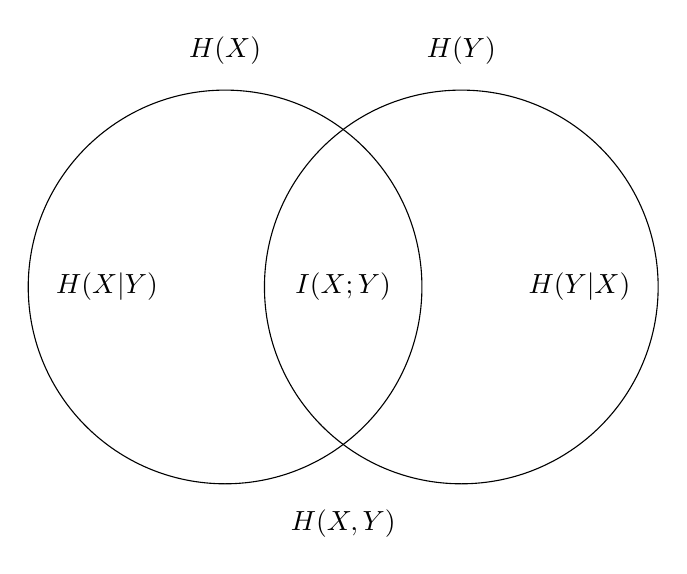
\begin{tikzpicture}
	\draw (0,0) circle (2.5cm);
	\draw (3,0) circle (2.5cm);
	
	\node (I)   at (1.5,0) {$I(X;Y)$}; 
	\node (HXY) at (-1.5,0) {$H(X|Y)$};
	\node (HYX) at (4.5,0) {$H(Y|X)$};
	\node (H)   at (1.5,-3) {$H(X,Y)$};
	\node (HX)  at (0,3) {$H(X)$};
	\node (HY)  at (3,3) {$H(Y)$};
\end{tikzpicture}
\end{center}
%\caption{Venn diagram of entropy} \label{fig:Venn_entropy}
%\end{figure}






\subsection{Further properties}


\paragraph{Conditional mutual information}

The \Define{conditional relative entropy} $D(p(y|x) || q(y|x))$ is defined as
\begin{align*}
	D(p(y|x) || q(y|x)) &:= \sum_x p(x) \sum_y p(y|x) \log \frac{p(y|x)}{q(y|x)}\\
	&= \expectation_{p(x,y)} \left( \log \frac{p(Y|X)}{q(y|X)} \right).
\end{align*}
The \Define{conditional mutual information} of $X$ and $Y$ given $Z$ is defined as
\begin{align*}
	I(X;Y|Z) &:= H(X|Z) - H(X|Y,Z)\\
	&= \expectation_{p(x,y,z)} \left( \log \frac{p(X,Y|Z)}{p(X|Z)p(Y|Z)} \right).
\end{align*}


\paragraph{Longer chain rules}

\begin{theorem}
Let $X_1,\ldots,X_n$ and $Y$ be random variables. Then
\begin{align*}
	H(X_1,\ldots,X_n) &= \sum_{i=1}^n H(X_i | X_{i-1}, \ldots, X_1)\\
	I(X_1,\ldots,X_n; Y) &= \sum_{i=1}^n I(X_i; Y | X_{i-1}, \ldots, X_1).
\end{align*}
\end{theorem}






\paragraph{Information inequality}

\begin{theorem}
Let $p(x)$, $q(x)$, $x \in \alphabet{X}$ be two probability mass functions. Then
\[
	D(p||q) \ge 0
\]
with equality if and only if $p(x) = q(x)$ for all $x$.
\end{theorem}

\begin{proof}
\begin{align*}
	-D(p||q) &= \expectation_p \left( \log \frac{q(x)}{p(x)} \right)\\
	&\le \log \expectation_p \left( \frac{q(x)}{p(x)} \right)\\
	&= \log \sum_x q(x)\\
	&\le 0.
\end{align*}
\end{proof}




\paragraph{Shannon's inequality}
\begin{corollary}[Non-negativity of mutual information]
For any two random variables $X$ and $Y$,
\[
	I(X;Y) \ge 0,
\]
with equality if and only if $X$ and $Y$ are independent.
\end{corollary}

Using a similar proof, we obtain results for the conditional mutual information.

\begin{corollary}[Shannon's inequality]
$D(p(y|x) || q(y|x)) \ge 0$ with equality if and only if $p(y|x) = q(y|x)$ for all $y$ and $x$ with $p(x) > 0$. Thus,
\[
	I(X;Y|Z) \ge 0,
\]
with equality if and only if $X$ and $Y$ are conditionally independent given $Z$.
\end{corollary}



\paragraph{More inequalities}
\begin{theorem}
$H(X) \le \log |\alphabet{X}|$, with equality if and only if $X$ has a uniform distribution over $\alphabet{X}$.
\end{theorem}

\begin{proof}
Let $u(x) = \frac{1}{|\alphabet{X}|}$ be the uniform distribution on $\alphabet{X}$, then
$$
	H(X) = \log |\alphabet{X}| - D(p||u) \le \log |\alphabet{X}|.
$$
\end{proof}

\begin{theorem}[Conditioning reduces entropy]
$$
	H(X|Y) \le H(X)
$$
with equality if and only if $X$ and $Y$ are independent.
\end{theorem}





\subsection{Exercises}


\begin{exercise}[Example of entropy]
Let $X$ and $Y$ be random variables on $\{x_0,x_1\}$ and $\{y_0,y_1\}$, respectively. They have the following joint distribution:
\begin{align*}
	p(x_0,y_0) &= 0\\
	p(x_0,y_1) &= \frac{1}{8}\\
	p(x_1,y_0) &= \frac{3}{4}\\
	p(x_1,y_1) &= \frac{1}{8}.
\end{align*}

Calculate $H(X)$, $H(Y)$, $H(X,Y)$ and $I(X;Y)$.
\end{exercise}



\begin{exercise}
Prove that for any random variables $X_1,\ldots,X_n$,
$$
	H(X_1,\ldots,X_n) \le \sum_{i=1}^n H(X_i),
$$
with equality if and only if the $X_i$ are independent.
\end{exercise}



\begin{exercise}[Entropy of functions of a random variable] 
Let $X$ be a discrete random variable and $g(X)$ be any function of that variable. Show that
$$
	H(X) \ge H(g(X)).
$$
In other words, processing data cannot increase the amount of information.
Hint: compute $H(X,g(X))$ in two different ways.
\end{exercise}



Random variables $X$, $Y$, and $Z$ are said to form a \Define{Markov chain} in that order (denoted as $X \to Y \to Z$) if the joint probability mas function can be written as
$$
	p(x,y,z) = p(x) p(y|x) p(z | y).
$$

In other words, each variable only depends on the preceding variable in the chain: $Z$ depends on $Y$, $Y$ depends on $X$, and $X$ is independent from $Y$ and $Z$.

\begin{exercise}
Prove that if $Z = f(Y)$, then $X \to Y \to Z$.
\end{exercise}


\begin{exercise}
Prove that $X$ and $Z$ are conditionally independent given $Y$, i.e.
$$
	p(x,z|y) = p(x|y) p(z|y).
$$
\end{exercise}








\begin{exercise}
Prove the following theorem and corollary, called the data processing inequality.

If $X \to Y \to Z$, then
\[
	I(X;Y) \ge I(X;Z).
\]
In particular, if $Z = g(Y)$, then $I(X;Y) \ge I(X;g(Y))$.

Why is this called the data processing inequality?
\end{exercise}









\section{Capacity I: Definition and examples}
\label{sec:33}




\subsection{Definition}

\paragraph{A communication system}
A source produces a message $W$, encodes it into a sequence $X^n$ and sends it through a channel.\\
~\\
The receiver obtains a corrupted version $Y^n$ and decodes it to some estimate $\hat{W}$ of $W$.

\begin{center}
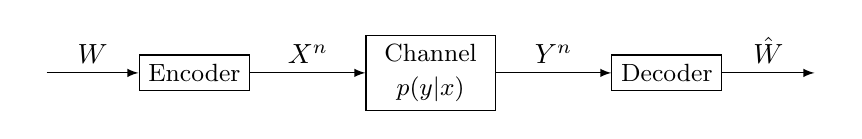
\begin{tikzpicture}[auto]
	\node (s) at (0,0) {}; %{\small{Message}};
	\node[draw] (e) at (2,0) {\small{Encoder}};
	\node[draw, text width=4em, text badly centered] (c) at (5,0) {\small{Channel} \small{$p(y|x)$}};
	\node[draw] (d) at (8,0) {\small{Decoder}};
	\node (r) at (10,0) {}; %{\small{Estimate}};
	
	\draw[-latex] (s) to node {$W$} (e);
	\draw[-latex] (e) to node {$X^n$} (c);
	\draw[-latex] (c) to node {$Y^n$} (d);
	\draw[-latex] (d) to node {$\hat{W}$} (r);
\end{tikzpicture}
\end{center}





\paragraph{Discrete channel}


A \Define{discrete channel} consists of an input alphabet $\alphabet{X}$, and output alphabet $\alphabet{Y}$, and a probability transition matrix $p(y | x)$ that expresses the probability of observing the output symbol $y$ given that we send the symbol $x$.

The channel is called \Define{memoryless} if the probability distribution of the output only depends on the input at that time and is conditionally independent of previous inputs or outputs.

The \Define{channel capacity} of a discrete memoryless channel is defined as
\[
	C = \max_{p(x)} I(X;Y).
\]

Intuitively, the mutual information $I(X.Y)$ is the amount of information the output $Y$ has about the input $X$: that's the amount of information that has been successfully transmitted through the channel. Changing the input distribution $p(x)$ amounts to different sorts of ``encoding'' the data: finding the best input that allows for the most information transmitted through the channel.

The mathematical definition of the capacity makes sense: for a given channel, the output probability distribution $p(y)$ is a function of the input probability distribution $p(x)$:
\[
    p(y) = \sum_x p(x) p(y | x),
\]
and hence the mutual information $I(X;Y)$ is a function of $p(x)$.

\subsection{Examples}

\paragraph{Noiseless binary channel}
Suppose that the channel can carry one bit and it is perfect: $p(y|x) = 1$ if $y=x$. Then $I(X;Y) = H(X)$, which is maximised for $p(x) = (1/2, 1/2)$. 
Thus,
$$
	C = 1.
$$ 



\paragraph{Noisy typewriter}
The alphabet is $\mathbb{Z}_{2q}$ and the input is either unchanged with probability $1/2$ or turned to the next symbol with probability $1/2$:
$$
	p(x|x) = p(x+1 \mod 2q | x) = \frac{1}{2}.
$$

(give figure.)

\begin{theorem}
The \Important{capacity of the noisy typewriter} is $\log q$.
\end{theorem}

\begin{proof}
The proof contains two parts. 

Firstly, we prove that the mutual information is always upper bounded by $\log q$. We have
\begin{align*}
	I(X;Y) &= H(Y) - H(Y|X)\\
	&= H(Y) - 1 \le \log (2q) - 1 = \log q.
\end{align*}

The second part is to exhibit an input distribution that matches our upper bound. Here, we reach capacity if we send every other symbol equiprobably, i.e. 
\[
	p(x) = \begin{cases}
	\frac{1}{q} & \text{if } x \equiv 0 \mod 2\\
	0 & \text{if } x \equiv 1 \mod 2,
	\end{cases}
\]
then we see that $H(X) = \log q$ and $H(Y) = \log(2q)$.
\end{proof}



\paragraph{Binary symmetric channel}

\Important{Binary Symmetric Channel}: $x, y \in \{0,1\}$, 
$$
	p(x|x) = 1-p, \quad p(1- x|x) = p.
$$

(give figure)


(Give figure and intuition behind several data points.)

The capacity $C(p)$ of the BSC has a few intuitive properties.
\begin{enumerate}
    \item $C(0) = 1$: in this case the channel is perfect.
    
    \item $C(p) = C(1-p)$: making that switch amounts to changing the roles of $0$ and $1$ at the destination.
    
    \item $C(1/2) = 0$: in this case, $Y$ receives random noise.
\end{enumerate}

\begin{theorem}
The capacity of a BSC with crossover probability $p$ is
\[
	C(p) = 1 - H(p).
\]
\end{theorem}


\begin{proof}
$$
	I(X;Y) = H(Y) - H(p) \le 1 - H(p),
$$
with equality if and only if $H(Y) = 1$, which is achieved when the input has a uniform distribution. 
\end{proof}



\subsection{The channel coding theorem}



\begin{definition}
The $n$-th extension of the discrete memoryless channel (DMC) is the channel $(\alphabet{X}^n, p(y^n | x^n), \alphabet{Y}^n)$, where
$$
	p(y_k | x^k, y^{k-1}) = p(y_k | x_k), \quad k=1,\ldots,n.
$$
\end{definition}

We shall use the channel without feedback, i.e. $p(x_k | x^{k-1}, y^{k-1}) = p(x_k | x^{k-1})$ hence
$$
	p(y^n | x^n) = \prod_{i=1}^n p(y_i | x_i).
$$





\begin{definition}
An $(M,n)$ \Structure{code} for the channel $(\alphabet{X}, p(y|x), \alphabet{Y})$ consists of the following:
\begin{enumerate}
	\item An index set $\{1,\ldots,M\}$.
	
	\item An encoding function $X^n : \{1,\ldots,M\} \to \alphabet{X}^n$, yielding codewords $X^n(1), \ldots, X^n(M)$. The set of codewords is called the codebook.
	
	\item A decoding function $g: \alphabet{Y}^n \to \{1,\ldots,M\}$.
\end{enumerate}
\end{definition}

The \Structure{rate} of an $(M,n)$ code is
$$
	R := \frac{\log M}{n} \, \text{bits per transmission.}
$$



\begin{definition}
Conditional probability of error 
\begin{align*}
	\lambda_w &:= \mathrm{Pr}\{g(Y^n) \ne w | X^n = X^n(w)\}\\
	&= \sum_{y^n : g(y^n) \ne w} p(y^n | x^n(w))
\end{align*}

\Structure{Maximal probability of error} $\lambda^{(n)}$ for an $(M,n)$ code is 
$$
	\lambda^{(n)} := \max \{\lambda_w : w \in \{1,\ldots,M\} \}.
$$
\end{definition}

We say a rate $R$ is \Structure{achievable} if there exists a sequence of $(2^{nR}, n)$ codes s.t. $\lambda^{(n)} \to 0$.



The channel coding theorem states that the channel capacity is equal to the maximum rate with which we can transmit data reliably (i.e., with negligible probability of error).

\begin{theorem}[The channel coding theorem]
All rates below capacity $C$ are achievable.\\
Specifically, for every rate $R < C$, there exists a sequence of $(2^{nR}, n)$ codes with maximum probability of error $\lambda^{(n)} \to 0$.\\
~\\
Conversely, any sequence of $(2^{nR}, n)$ codes with $\lambda^{(n)} \to 0$ must have $R \le C$.
\end{theorem}









% %\title{Capacity II\\ The channel coding theorem}

% \subsection{The theorem}

% \paragraph

% \begin{definition}
% The $n$-th extension of the discrete memoryless channel (DMC) is the channel $(\alphabet{X}^n, p(y^n | x^n), \alphabet{Y}^n)$, where
% $$
% 	p(y_k | x^k, y^{k-1}) = p(y_k | x_k), \quad k=1,\ldots,n.
% $$
% \end{definition}

% We shall use the channel without feedback, i.e.
% $$
% 	p(y^n | x^n) = \prod_{i=1}^n p(y_i | x_i).
% $$

% 

% \paragraph

% \begin{definition}
% An $(M,n)$ code for the channel $(\alphabet{X}, p(y|x), \alphabet{Y})$ consists of the following:
% \begin{enumerate}
% 	\item An index set $\{1,\ldots,M\}$.
	
% 	\item An encoding function $X^n : \{1,\ldots,M\} \to \alphabet{X}^n$, yielding codewords $X^n(1), \ldots, X^n(M)$. The set of codewords is called the codebook.
	
% 	\item A decoding function $g: \alphabet{Y}^n \to \{1,\ldots,M\}$.
% \end{enumerate}
% \end{definition}

% The rate of an $(M,n)$ code is
% $$
% 	R := \frac{\log M}{n} \, \text{bits per transmission.}
% $$
% 

% \paragraph
% \begin{definition}
% Conditional probability of error 
% \begin{align*}
% 	\lambda_w &:= \mathrm{Pr}\{g(Y^n) \ne w | X^n = X^n(w)\}\\
% 	&= \sum_{y^n : g(y^n) \ne w} p(y^n | x^n(w))
% \end{align*}

% \Structure{Maximal probability of error} $\lambda^{(n)}$ for an $(M,n)$ code is 
% $$
% 	\lambda^{(n)} := \max \{\lambda_w : w \in \{1,\ldots,M\} \}.
% $$
% \end{definition}

% We say a rate $R$ is \Structure{achievable} if there exists a sequence of $(2^{nR}, n)$ codes s.t. $\lambda^{(n)} \to 0$.\\
% ~\\
% Average probability of error $P_e^{(n)} := \frac{1}{M} \sum_w \lambda_w$.


% 


% \paragraph

% \begin{theorem}[The channel coding theorem]
% All rates below capacity $C$ are achievable.\\
% Specifically, for every rate $R < C$, there exists a sequence of $(2^{nR}, n)$ codes with maximum probability of error $\lambda^{(n)} \to 0$.\\
% ~\\
% Conversely, any sequence of $(2^{nR}, n)$ codes with $\lambda^{(n)} \to 0$ must have $R \le C$.
% \end{theorem}

% 






% \subsection{The Asymptotic Equipartition Property (AEP)}

% \paragraph{The Asymptotic Equipartition Property}

% Analogue of the law of large numbers for information theory.\\
% ~\\
% Context: an information source with probability distribution $p(x)$ keeps producing random variables $X_1,\ldots,X_n$ i.i.d with distribution $p(x)$.\\ 
% ~\\
% Claim: For $n$ large, almost all sequences $X_1,\ldots,X_n$ are very similar, and their behaviour is dictated by the entropy.
% 

% \paragraph{The AEP}

% \begin{theorem}[AEP]
% If $X_1,X_2,\ldots$ are i.i.d $\sim p(x)$, then
% $$
% 	- \frac{1}{n} \log p(X_1,\ldots, X_n) \to H(X) \quad \text{in probability.}
% $$
% \end{theorem}

% \begin{proof}
% Since the $X_i$ are i.i.d, so are $\log p(X_i)$. The weak law of large numbers gives
% \begin{align*}
% 	- \frac{1}{n} \log p(X_1,\ldots,X_n) &= - \frac{1}{n} \sum_i \log p(X_i)\\
% 	&\to -\mathrm{E} \log p(X) \quad \text{in probability}\\
% 	&= H(X).
% \end{align*}
% \end{proof}

% 

% \paragraph{Typical sets}

% \begin{definition}
% The \Structure{typical set} $A_\epsilon^{(n)}$ w.r.t. $p(x)$ is the set of sequences $x^n = (x_1,\ldots,x_n) \in \alphabet{X}^n$ such that
% 	$$
% 		H(X) - \epsilon \le -\frac{1}{n} \log p(x^n) \le H(X) + \epsilon.
% 	$$
% \end{definition}

% \begin{theorem}[The AEP for Typical Sequences]
% \begin{enumerate}
% 	\item $\mathrm{Pr}\{A_\epsilon^{(n)}\} \ge 1 - \epsilon$ for $n$ large enough.
	
% 	\item $|A_\epsilon^{(n)}| \le 2^{n(H(X) + \epsilon)}$.
	
% 	\item $|A_\epsilon^{(n)}| \ge (1- \epsilon) 2^{n(H(X) - \epsilon)}$ for $n$ large enough.
% \end{enumerate}
% \end{theorem}

% The typical set has probability nearly $1$, all elements of the typical set are nearly equiprobable, and the number of elements in the typical set is nearly $2^{nH(X)}$.

% 

% %\paragraph{Proof of the AEP}
% %
% %\begin{proof}
% %We've already proved Property 1.\\
% %~\\
% %Property 2:
% %\begin{align*}
% %	1 &= \sum_{x^n \in \alphabet{X}^n} p(x^n)\\
% %	&\ge \sum_{x^n \in A_\epsilon^{(n)}} p(x^n)\\
% %	&\ge \sum_{x^n \in A_\epsilon^{(n)}} 2^{-n(H(X) + \epsilon)}\\
% %	&= 2^{-n(H(X) + \epsilon)} |A_\epsilon^{(n)}|.
% %\end{align*}
% %\end{proof}
% %
% %
% %
% %\paragraph
% %Property 3: let $n$ large enough, then
% %\begin{align*}
% %	1- \epsilon &< \mathrm{Pr}\{A_\epsilon^{(n)}\}\\
% %	&\le \sum_{x^n \in A_\epsilon^{(n)}} 2^{-n(H(X) - \epsilon)}\\
% %	&= 2^{-n(H(X) - \epsilon)} |A_\epsilon^{(n)}|.
% %\end{align*}
% %
% %


% \paragraph{Example of the AEP}
% Consider $n$ coin flips $X_1,\ldots,X_n$, where heads (1) has probability $p$ and tails (0) probability $1-p$.\\
% We expect to see around $np$ heads on average, and all runs with roughly $np$ heads are nearly equiprobable.\\ 
% ~\\
% For any sequence $x^n \in\{0,1\}^n$ with $w$ heads,
% $$
% 	p(x^n)  = p^w (1-p)^{n-w}.
% $$

% The AEP indeed yields
% $$
% 	-\frac{1}{n} \log p(X_1,\ldots,X_n) \to H(p)
% $$
% and more precisely, for typical sets and $n$ large enough:
% \begin{align*}
% 	A_\epsilon^{(n)} &= \{x^n : |w - np| \le \epsilon n/ |\log p - \log (1-p)|\}\\
% 	\mathrm{Pr}\{A_\epsilon^{(n)}\} &\ge 1-\epsilon\\
% 	(1- \epsilon) 2^{n(H(p) - \epsilon)} &\le |A_\epsilon^{(n)}| \le 2^{n(H(p) + \epsilon)}.
% \end{align*}
% 



% %\paragraph{AEP and data compression}
% %???Give this as a practical exercise.
% %
% %Let $X_1,\ldots, X_n$ be i.i.d. We want a short description of this sequence. 
% %
% %\begin{theorem}
% %Let $X^n$ be i.i.d $\sim p(x)$ and $\epsilon > 0$. Then there exists a code which maps sequences $x^n$ of length $n$ into binary strings of length $l(x^n)$ such that the encoding is one-to-one and
% %$$
% %	\mathrm{E} \left[ \frac{1}{n}l(X^n) \right] \le H(X) + \epsilon.
% %$$
% %\end{theorem}
% %
% %Idea of proof:
% %\begin{enumerate}
% %	\item Split $\alphabet{X}^n$ into typical sequences (in $A_\epsilon^{(n)}$) and atypical ones.
% %	
% %	\item In $A_\epsilon^{(n)}$, encode using at most $\log |A_\epsilon^{(n)}| +1 \le n(H(X) + \epsilon) + 1$ bits.
% %	
% %	\item Use brute force enumeration of atypical ones (unimportant: they are unlikely to occur).
% %\end{enumerate}
% %
% %


% \paragraph{The joint AEP}

% \begin{definition}
% $A_\epsilon^{(n)}$: set of jointly typical sequences $(x^n, y^n)$ w.r.t. $p(x,y)$,
% \begin{align*}
% 	A_\epsilon^{(n)} := &\Big\{ (x^n, y^n) \in \alphabet{X}^n \times \alphabet{Y}^n :\\
% 	& \left| -\frac{1}{n} \log p(x^n) - H(X) \right| < \epsilon,\\
% 	& \left| -\frac{1}{n} \log p(y^n) - H(Y) \right| < \epsilon,\\
% 	& \left| -\frac{1}{n} \log p(x^n, y^n) - H(X,Y) \right| < \epsilon \Big\},\\
% \end{align*}
% where
% $$
% 	p(x^n, y^n) = \prod_{i=1}^n p(x_i, y_i).
% $$
% \end{definition}

% 

% \paragraph{The joint AEP}
% \begin{theorem}[Joint AEP]
% Let $(X^n, Y^n)$ be $n$-sequences drawn i.i.d. according to $p(x^n, y^n)$. Then
% \begin{enumerate}
% 	\item $\mathrm{Pr}\{ (X^n, Y^n) \in A_\epsilon^{(n)}\} \to 1$ as $n \to \infty$.
	
% 	\item $|A_\epsilon^{(n)}| \le 2^{nH(X,Y) + \epsilon}$.
	
% 	\item If $(\tilde{X}^n, \tilde{Y}^n) \sim p(x^n) p(y^n)$, then
% 	$$
% 		\mathrm{Pr}\{ (\tilde{X}^n, \tilde{Y}^n) \in A_\epsilon^{(n)} \} \le 2^{-n(I(X;Y) - 3 \epsilon)}.
% 	$$
% 	Also, for $n$ large enough,
% 	$$
% 		\mathrm{Pr}\{ (\tilde{X}^n, \tilde{Y}^n) \in A_\epsilon^{(n)} \} \ge (1 - \epsilon) 2^{-n(I(X;Y) + 3 \epsilon)}.		
% 	$$
	
% \end{enumerate}
% \end{theorem}
% 


% \subsection{Achievability}

% \paragraph{Intuition}
% The channel coding theorem states that the channel capacity is equal to the maximum rate with which we can transmit data reliably (i.e., with negligible probability of error)\\
% ~\\
% Basic idea: for large block lengths, any channel looks like a noisy typewriter and the channel has a subset of inputs that produce essentially disjoint sequences at the output.\\
% ~\\
% For each typical input $n$-sequence there are roughly $2^{nH(Y|X)}$ possible $Y$ sequences, all of them equally likely.\\
% ~\\
% We wish to ensure that two different $X$ sequences produce different $Y$ sequences.\\
% ~\\
% There are roughly $2^{nH(Y)}$ typical $Y$ sequences, hence roughly $2^{nH(Y) - nH(Y|X)} = 2^{nI(X;Y)}$ different sets: code rate of $I(X;Y)$.
% 

% \paragraph
% We first prove that rates $R < C$ are achievable.\\
% ~\\
% Fix $p(x)$. Generate independently $2^{nR}$ codewords according to the distribution
% $$
% 	p(x^n) = \prod_{i=1}^n p(x_i).
% $$
% The codewords are represented as the rows of a matrix
% $$
% 	\alphabet{C} = \begin{pmatrix}
% 	x_1(1) & \ldots  & x_n(1)\\
% 	\vdots & \vdots & \vdots\\
% 	x_1(2^{nR}) & \ldots & x_n(2^{nR})
% 	\end{pmatrix}
% $$
% The probability of generating a particular code $\alphabet{C}$ is 
% $$
% 	\mathrm{Pr}\{\alphabet{C}\} = \prod_{w=1}^{2^{nR}} \prod_{i=1}^n p(x_i(w)).
% $$
% 

% \paragraph
% Consider the following sequence of events:
% \begin{enumerate}
% 	\item A \Structure{random code} $\alphabet{C}$ is generated.
	
% 	\item Sender and receiver know $\alphabet{C}$ and the channel $p(y|x)$.
	
% 	\item A message $W$ is chosen according to a uniform distribution
% 	$$
% 		\mathrm{Pr}\{W = w\} = 2^{-nR}, \quad w=1,\ldots,2^{nR}.
% 	$$
	
% 	\item The $w$-th codeword $X^n(w)$ is sent over the channel.
	
% 	\item The receiver receives $Y^n$ according to
% 	$$
% 		p(y^n | x^n(w)) = \prod_{i=1}^n p(y_i | x_i(w)).
% 	$$
	
% 	\item The receiver guesses which message was sent using \Structure{typical set decoding}: he declares that $\hat{W}$ was sent if 
% 	\begin{itemize}
% 		\item $(X^n(\hat{W}), Y^n)$ is joint typical and
		
% 		\item $(X^n(w), Y^n)$ is not jointly typical for any other $w$.
% 	\end{itemize}
	
% 	\item Decoding error if $\hat{W} \ne W$. Let $E$ be the error event.
% \end{enumerate}

% 

% \paragraph{Analysis of Probability of error}

% Idea: consider the average over all codes.\\
% %
% %We have
% %\begin{align*}
% 	%Pr(\alphabet{E}) &= \sum_{\alphabet{C}} P(\alphabet{C}) P_e^{(n)} (\alphabet{C})\\
% 	%&= \sum_{\alphabet{C}} P(\alphabet{C}) \frac{1}{2^{nR}} \sum_{w=1}^{2^{nR}} \lambda_w(\alphabet{C})\\
% 	%&= \frac{1}{2^{nR}} \sum_{w=1}^{2^{nR}} \sum_{\alphabet{C}} P(\alphabet{C}) \lambda_w(\alphabet{C}).
% %\end{align*}
% ~\\
% By symmetry of the code construction, the average probability of error averaged over all codes does not depend on the particular index that was sent.\\
% ~\\
% So, let us assume $W=1$ was transmitted. We obtain
% \begin{align*}
% 	\mathrm{Pr}\{E\} &= \sum_{\alphabet{C}} P(\alphabet{C}) P_e^{(n)} (\alphabet{C})\\
% 	&= \mathrm{Pr}\{E | W=1\}.
% \end{align*}

% 

% \paragraph
% Denoting the event $E_w := \{(X^n(w), Y^n) \in A_\epsilon^{(n)}\}$, we have
% \begin{align*}
% 	\mathrm{Pr}\{E | W=1\} &= P(E^c_1 \cup E_2 \cup \ldots \cup E_{2^{nR}})\\
% 	&\le P(E_1^c) + \sum_{w=2}^{2^{nR}} P(E_w).
% \end{align*}

% By the joint AEP, $P(E_1^c) \le \epsilon$ for $n$ large enough.\\
% ~\\
% By the code generation, $X^n(1)$ and $X^n(i)$ are independent, so are $Y^n$ and $X^n(w)$, $w \ne 1$. Hence by the joint AEP,
% $$
% 	P(E_w) \le 2^{-n(I(X;Y) - 3 \epsilon)},
% $$
% whence
% $$
% 	\mathrm{Pr}\{E\} \le 2 \epsilon
% $$
% for $R < I(X;Y) - 3 \epsilon$ and $n$ large enough.
% 

% \paragraph
% We finish the proof as such.
% \begin{enumerate}
% 	\item Choose $p(x)$ which achieves capacity: this replaces $I(X;Y)$ with $C$.
	
% 	\item Get rid of average over codebooks. There exists a codebook $\alphabet{C}$ with average error $\le 2 \epsilon$.
	
% 	\item Throw away half the codewords in $\alphabet{C}$ (the ones with highest $\lambda_w$) to obtain $\alphabet{C}^*$.\\
% 	We have $\lambda^{(n)}(\alphabet{C}^*) \le 4 \epsilon$ and the rate of $\alphabet{C}^*$ is $R - \frac{1}{n} \to R$.
% \end{enumerate}
% 



% \subsection{Converse}

% \paragraph{Fano's inequality}
% The decoder wishes to estimate $X$ with distribution $p(x)$. They observe $Y$, related to $X$ by the conditional distribution $p(y|x)$.\\
% ~\\
% From $Y$, they calculate an estimate $g(Y) = \hat{X}$ of $X$.\\
% ~\\
% Let the probability of error be 
% \[
% 	P_e := \mathrm{Pr}\{ \hat{X} \ne X\}.
% \]

% Fano's inequality relates $P_e$ to $H(X|Y)$.

% \begin{theorem}[Fano's inequality]
% \[
% 	H(P_e) + P_e \log(|\alphabet{X}| - 1) \ge H(X|Y).
% \]
% \end{theorem}
% 

% %This can be weakened to
% %\begin{align*}
% %	1 + P_e \log |\alphabet{X}| &\ge H(X|Y)\\
% %	P_e &\ge \frac{H(X|Y) - 1}{\log |\alphabet{X}|}.
% %\end{align*}


% \paragraph{Proof of Fano's inequality}
% Define an error random variable
% \[
% 	E = \begin{cases}
% 	1 & \mbox{if } \hat{X} \ne X\\
% 	0 & \mbox{if } \hat{X} = X.
% 	\end{cases}
% \]

% By the Venn diagram of entropy,
% \[
% 	H(X|Y) = H(E|Y) + H(X|E,Y) - H(E|X,Y).
% \]

% However,
% \begin{align*}
% 	H(E|X,Y) &= 0,\\
% 	H(E|Y) &\le H(E) = H(P_e),\\
% 	H(X|E,Y) &= (1-P_e) H(X|Y,E=0) + P_e H(X|Y,E=1)
% 	\le P_e \log(|\alphabet{X}| - 1).
% \end{align*}

% Thus $H(X|Y) \le H(P_e) + P_e \log(|\alphabet{X}| - 1)$.
% 




% \paragraph{Converse to the coding theorem}

% We will show that if the probability of error tends to zero, then the code rate must be at most $C$.

% \begin{lemma}[Fano's inequality]
% For a DMC with a codebook $\alphabet{C}$ and the input messages uniformly distributed, let $P_e^{(n)} = \mathrm{Pr}\{W \ne g(Y^n)\}$. Then
% $$
% 	H(W | Y^n) \le 1 + P_e^{(n)} n R.
% $$
% \end{lemma}

% We can easily show that using the channel multiple times does not increase the capacity.

% \begin{lemma}
% Let $Y^n$ be the result of passing $X^n$ through a DMC. Then
% $$
% 	I(X^n; Y^n) \le nC.
% $$
% \end{lemma}


% 


% \paragraph{Proof of converse}

% If $\lambda^{(n)} \to 0$, then $P_e^{(n)} \to 0$.\\
% ~\\
% For each $n$, let $W$ be drawn according to a uniform distribution, then $P_e^{(n)} = \mathrm{Pr}\{\hat{W} \ne W\}$ and
% \begin{align*}
% 	nR &= H(W) = H(W|Y^n) + I(W;Y^n)\\
% 	&\le 1 + P_e^{(n)} nR + nC.
% \end{align*}
% Divide by $n$, take the limit:
% $$
% 	R \le C.
% $$

% 

% %\paragraph{Strong converse}
% %We showed that
% %$$
% %	P_e^{(n)} \ge  1- \frac{C}{R} - \frac{1}{nR} \to 1 - \frac{C}{R}.
% %$$
% %Therefore, if the rate is higher than the capacity, the probability of error is bounded away from zero.\\
% %~\\
% %In fact, there is a \Structure{strong converse}: if $R > C$, then $P_e^{(n)} \to 1$ exponentially. The capacity is a clear dividing point!
% %

\subsection{See further}

Sketch of the proof of achievability?



\subsection{Exercises}

\begin{exercise}
Determine the capacity of the following additive channel, where $X \in \{0,1\}$ and $\mathrm{Pr}\{Z = 0\} = \mathrm{Pr}\{Z = a\} = \frac{1}{2}$ for some real number $a > 0$.\\
~\\
\begin{center}
\begin{tikzpicture}
	\node (x) at (0,0) {$X$};
	\node (y) at (4,0) {$Y$};
	\node (z) at (2,2) {$Z$};
	\node[draw, shape=circle] (p) at (2,0) {$+$};
	
	\draw[-latex] (x) -- (p);
	\draw[-latex] (z) -- (p);
	\draw[-latex] (p) -- (y);
\end{tikzpicture}
\end{center}
\end{exercise}

\begin{remark}
We also use the notation 
$$
	Z = \begin{pmatrix}
		0, & a\\
		\frac{1}{2}, & \frac{1}{2}
	\end{pmatrix}.
$$
\end{remark}



\begin{exercise}
The Z-channel with error probability $p$, also called binary asymmetric channel, is a channel where the transition $0 \to 1$ never occurs.

\begin{center}
\begin{tikzpicture}[auto]
	\node (s0) at (0,3) {$0$};
	\node (s1) at (0,0) {$1$};
	\node (d0) at (3,3) {$0$};
	\node (d1) at (3,0) {$1$};
	
	\node (x) at (-1,1.5) {$X$};
	\node (y) at (4,1.5) {$Y$};
	
	\draw[-latex] (s0) -- (d0);
	\draw[-latex] (s1) to node[pos=0.3] {$p$} (d0);
	\draw[-latex] (s1) to node {$1-p$} (d1);
\end{tikzpicture}
\end{center}

What is the capacity of this channel?
\end{exercise}














\section{Capacity II: Multiple access and broadcast channels}
\label{sec:34}

\paragraph{Network information theory}
A system with many senders and many receivers contains many new elements in the communication problem: interference, cooperation and feedback. These issues are the domain of \Structure{Network Information Theory}.

\Structure{Problem:} given many senders and receivers and a channel transition matrix which describes the effects of the interference and the noise in the network, determine whether or not the sources can be transmitted over the channel. This requires determining the capacity region of the network.

Determining the capacity region of systems with multiple senders/receivers is the main challenge of research in information theory nowadays. We will only look at some very special cases.




\subsection{Multiple access channel}

\paragraph{Definition}

A \Define{Multiple Access Channel} consists of three alphabets $\alphabet{X}_1, \alphabet{X}_2, \alphabet{Y}$ and a probability transition matrix $p(y | x_1, x_2)$. Thus, there are two senders and one receiver on this channel.


\begin{center}
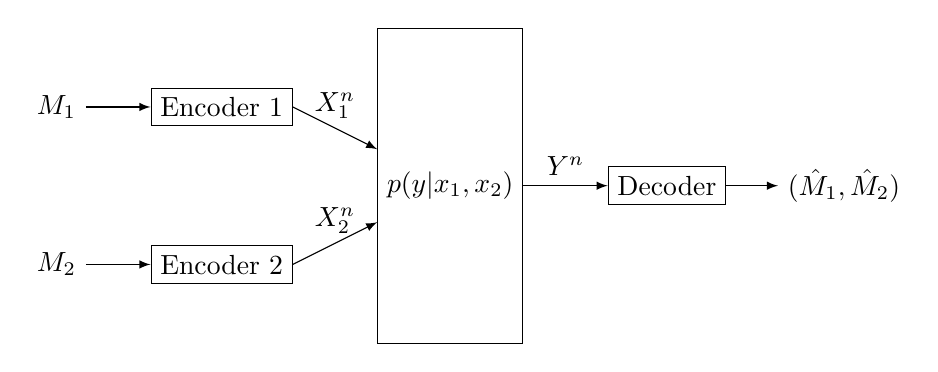
\begin{tikzpicture}
	%\draw (0,0) rectangle (4,4);
	
	\node 							(M1)	at (0,3)	{$M_1$};
	\node 							(M2)	at (0,1)	{$M_2$};
	\node[draw, left] 				(E1)	at (3,3) 	{Encoder 1};
	\node[draw, left] 				(E2)	at (3,1) 	{Encoder 2};
	\node[draw, minimum height=4cm]	(C)		at (5,2) 	{$p(y|x_1, x_2)$};
	\node[draw, right] 				(Dec)	at (7,2) 	{Decoder};
	\node 							(HM)	at (10,2) 	{$(\hat{M}_1, \hat{M}_2)$};
	
	\draw[-latex] (M1) 	-- (E1);
	\draw[-latex] (M2) 	-- (E2);
	\draw[-latex] (E1.east) -- (C) node[pos=0.5, above]{$X_1^n$};
	\draw[-latex] (E2.east) -- (C) node[pos=0.5, above]{$X_2^n$};
	\draw[-latex] (C)	-- (Dec.west) node[pos=0.5, above]{$Y^n$};
	\draw[-latex] (Dec)	-- (HM);

\end{tikzpicture}
\end{center}

\paragraph{Codes}

A $((2^{nR_1}, 2^{nR_2}), n  )$ code for the MAC consists of two sets of integers $\alphabet{W}_1 = \{ 1, 2, \dots, 2^{nR_1} \}$ and $\alphabet{W}_2 = \{ 1, 2, \dots, 2^{nR_2} \}$ called the messages sets and two encoding functions
\begin{align*}
	X_1 : \alphabet{W}_1 \to \alphabet{X}_1^n,\\
	X_2 : \alphabet{W}_2 \to \alphabet{X}_2^n,
\end{align*}
and a decoding function 
\[
	g: \alphabet{Y}^n \to \alphabet{W}_1 \times \alphabet{W}_2.
\]
The average probability of error is
\[
	P_e^{(n)} = \frac{1}{2^{nR_1 + nR_2}} \sum_{(w_1, w_2) \in \alphabet{W}_1 \times \alphabet{W}_2} \probability( g(Y^n) \ne (w_1, w_2) | (w_1, w_2) \text{ was sent} ).
\]
A rate pair $(R_1, R_2)$ is \Define{achievable} if there exists a sequence of $((2^{nR_1}, 2^{R_2}), n  )$ codes with $P_e^{(n)} \to 0$.


\paragraph{Capacity region}
The \Structure{capacity region} of the MAC is the closure of the set of achievable $(R_1, R_2)$ rate pairs.

\begin{theorem}
The capacity region of a MAC $( \alphabet{X}_1 \times \alphabet{X}_2 , p(y | x_1, x_2), \alphabet{Y} )$ is the closure of the convex hull of all $(R_1, R_2)$ satisfying
\begin{align*}
	R_1 &< I(X_1 ; Y | X_2),\\
	R_2 &< I(X_2 ; Y | X_1),\\
	R_1 + R_2 &< I(X_1, X_2 ; Y)
\end{align*}
for some product distribution $p_1(x_1) p_2(x_2)$ on $\alphabet{X}_1 \times \alphabet{X}_2$.
\end{theorem}


\begin{center}
\begin{tikzpicture}
	
	\draw[-latex] (0,0) node[below left]{0} -- (5,0) node[below]{$R_1$};
	\draw[-latex] (0,0) -- (0,4) node[left]{$R_2$};
	
	\draw[thick] (0,3) node[left]{$C_2$} -- (2,3) -- (4,1) -- (4,0) node[below]{$C_1$};
		
\end{tikzpicture}
\end{center}


The inequality
\[
	R_1 + R_2 < I(X_1, X_2 ; Y)
\]
corresponds to viewing the channel as a single-user channel with source $(X_1, X_2)$. This inequality is simply  the channel coding theorem for that channel.

The inequality
\[
	R_1 < I(X_1; Y | X_2)
\]
means that once we know $X_2$, the channel then reduces to a single-user channel with source $X_1$. The channel coding theorem then yields $R_1 < I(X_1; Y | X_2)$. The inequality $R_2 < I(X_2; Y | X_1)$ is similar. 









\paragraph{Example: independent channels}
Assume that we have two independent BSC, one from sender 1 (with crossover probability $p_1$), the other from sender 2 (with $p_2$).\\
~\\
Since there is no interference between the senders, we can achieve any pair $(R_1, R_2)$ as long as each rate corresponds to each BSC.\\
~\\
Thus, the capacity region is then defined by the inequalities
\begin{align*}
	R_1 &\le 1 - H(p_1)\\
	R_2 &\le 1 - H(p_2).
\end{align*}











\paragraph{Binary multiplier channel}
In this case, $\alphabet{X}_1 = \alphabet{X}_2 = \alphabet{Y} = \{0,1\}$. The output is given by
\[
	Y = X_1 X_2.
\]
If $X_2 = 1$, then $Y = X_1$ and hence $X_1$ can transmit at a rate of $1$ bit per transmission. Thus $R_1 \le 1$ (and similarly, $R_2 \le 1$.)\\
~\\
Since $Y$ is binary, $R_1 + R_2 \le 1$. By timesharing, we can achieve any rate pair $(R, 1-R)$.\\
~\\
\Structure{Timesharing:} for any $n$ and $k \le n$, let 
\begin{align*}
	X_{1,1} \dots X_{1,k} &\text{ i.i.d} \sim B(1/2)\\
	X_{1,k+1} \dots X_{1,n} &= 1,\\
	X_{2,1} \dots X_{2,k} &= 1\\
	X_{2,k+1} \dots X_{2,n} &\text{ i.i.d} \sim B(1/2),\\
\end{align*}
This achieves a rate of $(k/n, 1-k/n)$.



\paragraph{Generalisation to $m$ users}
The situation is similar for $m \ge 2$ users.\\
~\\
Let $[m] = \{1, 2, \dots, m\}$. For any $S \subseteq [m]$, denote its complement as $\bar{S}$, denote $R_S = \sum_{i \in S} R_i$ and $X_S = \{ X_i: i \in S \}$.\\
~\\
\Structure{Theorem.} The capacity region of the $m$-user MAC is the closure of the convex hull of the rate vectors satisfying 
\[
	R_S \le I \left(  X_S; Y \ | \ X_{\bar{S}}  \right)
\]
for all $S \subseteq [m]$, for some product distribution $p_1(x_1) \dots p_m(x_m)$.



\subsection{Broadcast channel}

\paragraph{The broadcast channel}


\begin{center}
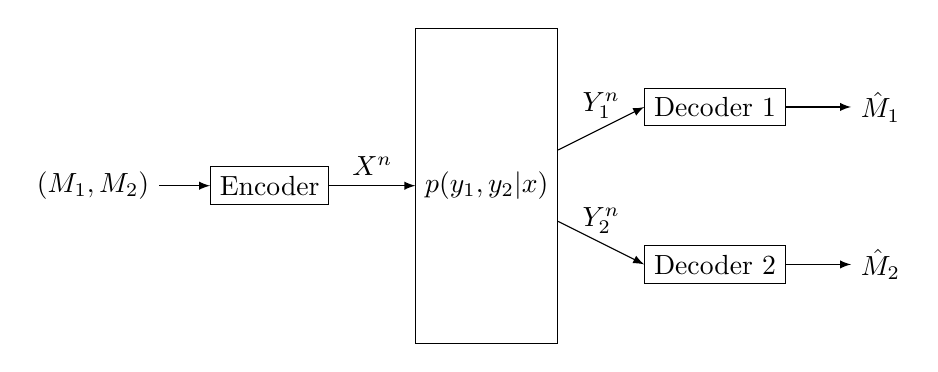
\begin{tikzpicture}
	%\draw (0,0) rectangle (4,4);
	
	\node 							(M)		at (0,2)	{$(M_1, M_2)$};
	\node[draw, left] 				(Enc)	at (3,2) 	{Encoder};
	\node[draw, minimum height=4cm]	(C)		at (5,2) 	{$p(y_1,y_2|x)$};
	\node[draw, right] 				(D1)	at (7,3) 	{Decoder 1};
	\node 							(HM1)	at (10,3) 	{$\hat{M}_1$};
	\node[draw, right] 				(D2)	at (7,1) 	{Decoder 2};
	\node 							(HM2)	at (10,1) 	{$\hat{M}_2$};
	
	\draw[-latex] (M) 	-- (Enc);
	\draw[-latex] (Enc) -- (C) node[pos=0.5, above]{$X^n$};
	\draw[-latex] (C)	-- (D1.west) node[pos=0.5, above]{$Y_1^n$};
	\draw[-latex] (D1)	-- (HM1);
	\draw[-latex] (C)	-- (D2.west) node[pos=0.5, above]{$Y_2^n$};
	\draw[-latex] (D2)	-- (HM2);
\end{tikzpicture}
\end{center}



\paragraph{Some definitions for the broadcast channel}
A broadcast channel consists of three alphabets $\alphabet{X}, \alphabet{Y}_1, \alphabet{Y}_2$ and a probability transition matrix $p(y_1, y_2 | x)$. The broadcast channel is memoryless if
\[
	p(y_1^n, y_2^n | x^n) = \prod_{i=1}^n p(y_{1i}, y_{2i} | x_i).
\]
$((2^{nR_1}, 2^{nR_2}), n)$ codes are defined as you might expect (with one encoder and two decoders this time).\\
~\\
The probability of error is ``disjunctive'':
\[
	P_e^{(n)} = \probability( g_1(Y_1^n) \ne M_1 \text{ or } g_2(Y_2^n) \ne M_2 ).
\]
~\\
A rate pair $(R_1, R_2)$ is achievable if there exists a sequence of codes with that rate pair and $P_e^{(n)} \to 0$.



\paragraph{Physically degraded broadcast channels}
A broadcast channel is called \Structure{physically degraded} if one of the following equivalent conditions is satisfied:
\begin{enumerate}
	\item $Y_2$ is a random degradation of $Y_1$;
	
	\item $X \to Y_1 \to Y_2$ (Markov chain);
	
	\item $p(y_1, y_2 | x) = p(y_1 | x) p(y_2 | y_1)$.
\end{enumerate}

\Structure{Theorem.} The capacity region for sending independent information over the degraded broadcast channel $X \to Y_1 \to Y_2$ is the convex hull of the closure of all $(R_1, R_2)$ satisfying
\begin{align*}
	R_2 &\le I(U; Y_2)\\
	R_1 &\le I(X; Y_1 | U),
\end{align*}
for some joint distribution $p(u) p(x | u) p(y_1, y_2 | x)$, where the auxiliary random variable $U$ is defined over $\alphabet{U}$ with $|\alphabet{U}| \le \min \{ |\alphabet{X}|, |\alphabet{Y}_1|, |\alphabet{Y}_2| \}$.




\paragraph{A bit of explanation}
The main idea is \Structure{superposition coding}.\\
~\\
The auxiliary variable $U$ serves as a cloud centre that can be distinguished by both $Y_1$ and $Y_2$.\\
~\\
Each cloud consists of $2^{nR_1}$ codewords $X^n$ distinguishable by the receiver $Y_1$.
$Y_2$ can only see the clouds, while $Y_1$ can see the individual codewords within the clouds.\\
~\\
Using superposition coding, one can achieve any rate pair s.t.
\begin{align*}
	R_2 &< I(U; Y_2),\\
	R_1 &\le I(X; Y_1 | U),\\
	R_1 + R_2 &< I(X; Y_1)
\end{align*}
for some $p(u,x)$.\\
~\\
(The bound on $|\alphabet{U}|$ follows from convex set theory; this is outside the scope of this lecture.)


\subsection{Exercises}



\begin{exercise}
Suppose the rate pairs $(R_1,R_2)$ and $(R'_1,R'_2)$ are achievable for a DM-MAC. Show that $(\lambda R_1 + (1- \lambda)R'_1, \lambda R_2 + (1- \lambda)R'_2)$ is also achievable for any $\lambda \in [0,1]$.
\end{exercise}



\begin{exercise}
Prove that the capacity region of the DM-BC depends on $p(y_1, y_2|x)$ only through the conditional marginal distributions $p(y_1|x)$ and $p(y_2|x)$.
\end{exercise}




\begin{exercise}
The Binary Symmetric Broadcast Channel (BS-BC) is a Broadcast channel where each receiver sees a BSC. It is illustrated below.

\begin{center}
\begin{tikzpicture}
	\node (X) 	at (0,2) {$X$};
	\node[draw, circle] (C1) 	at (2,3) {$+$};
	\node[draw, circle] (C2) 	at (2,1) {$+$};
	\node (D1) 	at (4,3) {$Y_1$};
	\node (D2) 	at (4,1) {$Y_2$};
	\node (Z1) 	at (2,4.5) {$Z_1 \sim B(p_1)$};
	\node (Z2) 	at (2,-0.5) {$Z_2 \sim B(p_2)$};
	
	\draw[-latex] (X) -- (1,2) -- (C1);
	\draw[-latex] (1,2) -- (C2);
	\draw[-latex] (Z1) -- (C1);
	\draw[-latex] (C1) -- (D1);
	\draw[-latex] (Z2) -- (C2);
	\draw[-latex] (C2) -- (D2);
\end{tikzpicture}
\end{center}

The noises $Z_1$ and $Z_2$ are independent; without loss, you may assume $p_1, p_2 \le 1/2$.

Prove that the BSC-BC is degraded.
\end{exercise}



\begin{exercise}
Prove that the whole capacity region of the degraded broadcast channel is indeed given by  superposition coding. You may use the results from the lecture.
\end{exercise}





\section{Compression I: Entropy coding}
\label{sec:35}



\subsection{Source codes}

\paragraph{Source code}

We wish to encode the values of a random variable $X$ into string of symbols over a finite alphabet $\alphabet{D} = \{0,1,\ldots,D-1\}$.\\
~\\
In this lecture, we will use $\alphabet{D} = \{0,1\}$, but the analysis is the same for any $D$.


A \Define{binary source code} for a random variable $X$ is a mapping $C : \alphabet{X} \to \{0,1\}^*$.

We denote the codeword corresponding to $x$ as $C(x)$ and its length as $l(x)$.\\
~\\
The \Define{expected length} of the code is
\[
	L(C) := \mathrm{E} l(x) = \sum_{x \in \alphabet{X}} p(x) l(x).
\]




\paragraph{Uniquely decodable codes}

Since we are going to encode  sequences of symbols $x_1 \ldots x_n$ from $X$, we need to make sure that no two sequences will be mapped to the same string of bits.\\
~\\
We denote $x^n = x_1 x_2 \ldots x_n$ and
$$
	C(x^n) := C(x_1) C(x_2) \ldots C(x_n)
$$
as the concatenation of these $n$ codewords.

\begin{definition}
The code is \Structure{uniquely decodable} if
$$
	x^n \ne y^m \Rightarrow C(x^n) \ne C(y^m).
$$
\end{definition}




\paragraph{Prefix codes}

The $i$-th prefix of $x^n = x_1 \ldots x_n$ is simply $x^i := x_1 \ldots x_i$.

\begin{definition}
A code is a \Structure{prefix code} (a.k.a. instantaneous code) if no codeword is a prefix of any other codeword.
\end{definition}
~\\
Clearly, a prefix code is uniquely decodable.








\subsection{Kraft inequality}

\paragraph{Binary trees}
A \Structure{binary tree} is a rooted tree where each parent has at most two children.\\
~\\
Prefix codes and binary trees are equivalent.\\
~\\
From a binary tree $T$, label the edges from a parent to each child as $0$ and $1$. Let the leaves be $\alphabet{X} = \{x_1, \dots, x_k \}$, then the code $C_T :\alphabet{X} \to \{0,1\}^*$ defined by the labels from the root to each leaf is a prefix code.\\
~\\
Conversely, from a prefix code $C$, it is easy to reconstruct a binary tree $T$ such that $C = C_T$.



\paragraph{Kraft sequences}
A (binary) \Structure{Kraft sequence} is a sequence of integers $l_1, \dots, l_k$ such that 
\[
	\sum_{i=1}^k 2^{-l_i} \le 1.
\]

Binary trees and Kraft sequences are equivalent.\\
~\\
From a binary tree $T$, let $L_T = l_1, \dots, l_k$ denote the respective depths of its leaves. Then it is easy to show that $l_T$ is a Kraft sequence.\\
~\\
Conversely, given any Kraft sequence $L = l_1, \dots, l_k$, we can construct a binary tree $T$ such that $L_T = L$ as follows.\\
~\\
Call the first node of depth $l_1$ as codeword $1$, and remove its descendants from the tree. Then call the first remaining node of level $l_2$ as codeword 2, etc.%\\
%~\\
%Exercise: build the tree for $(l_1,l_2,l_3,l_4) = (1,2,4,4)$.


\paragraph{The triple equivalence}

We have a triple equivalence
\[
	\text{Prefix code } C_T \sim \text{Binary tree } T \sim \text{Kraft sequence } L_T.
\]

As a result, the codeword lengths of any uniquely prefix code form a Kraft sequence, i.e.
$$
	\sum_{x \in \alphabet{X}} 2^{-l(x)} \le 1.
$$






\paragraph{Kraft inequality for uniquely decodable codes}

\begin{theorem}
The codeword lengths of any uniquely decodable code form a Kraft sequence, i.e.
$$
	\sum_{x \in \alphabet{X}} 2^{-l(x)} \le 1.
$$
%
%Conversely, given a set of codeword lengths which satisfy this inequality, it is possible to construct a prefix code with these codeword lengths.
\end{theorem}

Note: 
\begin{enumerate}
	\item The inequality was first proved by Kraft for prefix codes; it was then generalised to uniquely decodable codes by McMillan.
	
	\item This shows that prefix codes are the best kind of uniquely decodable codes.
\end{enumerate}


% \paragraph{Proof of the Kraft inequality}
% We prove $\sum_x 2^{-l(x)} \le 1 + \epsilon$ for any $\epsilon > 0$.\\
% ~\\
% Denote $l_{\max} := \max_{x \in \alphabet{X}} l(x)$ and let $k$ such that $(k l_{\max})^{1/k} \le 1 + \epsilon$.\\
% ~\\
% The number of sequences $x^k$ mapped to codewords of length $m$ satisfy 
% $$
% 	|\{x^k : l(x^k) = m\}| \le 2^m.
% $$

% We have
% \begin{align*}
% 	\left( \sum_{x \in \alphabet{X}} 2^{-l(x)} \right)^k &= \sum_{x^k \in \alphabet{X}^k} 2^{-l(x^k)}\\
% 	&= \sum_{m=1}^{kl_{\max}} |\{x^k : l(x^k) = m\}| \cdot 2^{-m}\\
% 	&\le k l_{\max}.
% \end{align*}
% Thus 
% \[
% 	\sum_{x \in \alphabet{X}} 2^{-l(x)} \le (k l_{\max})^{1/k} \le 1 + \epsilon.
% \]
% 




\subsection{Optimal codes}

\paragraph{The source coding theorem}

\begin{theorem}
Let $L^*$ be the minimum expected length of a binary uniquely decodable code for $X$. Then
$$
	H(X) \le L^* < H(X) + 1.
$$
\end{theorem}

\begin{proof}
We first prove the lower bound. We have
\begin{align*}
	H(X) - L^* &= \sum_i p_i \log \frac{1}{p_i} - \sum_i p_i l_i^* \\
	&= \sum_i p_i \log \frac{2^{-l_i*}}{p_i}\\
	&\le \log \sum_i p_i \frac{2^{-l_i*}}{p_i}\\
	&\le \log 1 = 0.
\end{align*}
\end{proof}



\paragraph{Shannon code}

For the upper bound, we use the converse of the Kraft inequality.\\
~\\
The \Structure{Shannon code} is a (suboptimal) code where
$$
	l(x) = \left\lceil \log \frac{1}{p(x)} \right\rceil.
$$
This is a Kraft sequence:
$$
	\sum_{x \in \alphabet{X}} 2^{-\left\lceil \log \frac{1}{p(x)} \right\rceil} \le \sum_{x \in \alphabet{X}} p(x) = 1.
$$
As such, the Shannon code always exists!\\
~\\
We have
\begin{align*}
	L^* &\le \sum_{x \in \alphabet{X}} p(x) \left\lceil \log \frac{1}{p(x)} \right\rceil\\
	&< \sum_{x \in \alphabet{X}} p(x) \left(\log \frac{1}{p(x)} + 1 \right)\\
	&< H(X) + 1.
\end{align*}

The practical will show how to construct the Shannon code.






\paragraph{Triple equivalence: optimal case}

Say a code $C$ is \Structure{optimal} if it achieves the minimum expected length for some probability distribution.\\
~\\
Say a binary tree is \Structure{optimal} if every parent has exactly two children.\\
~\\
Say a Kraft sequence is \Structure{optimal} if $\sum_{i=1}^k 2^{-l_i} = 1$.\\
~\\
Then for any binary tree $T$,
\[
	C_T \text{ is optimal } \iff T \text{ is optimal } \iff  L_T \text{ is optimal}.
\]



\subsection{Exercises}


\begin{exercise}
We have seen that the optimal expected length of a code is upper bounded by $H(X) + 1$. Show that this is tight, i.e. for any $\epsilon > 0$, give an example of a source $X$ for which the optimal length is at least $H(X) + 1 - \epsilon$.
\end{exercise}



\begin{exercise}
Prove the following theorem. 

\begin{theorem}\label{th:source_coding}
Let $X_1,\ldots,X_n$ be i.i.d. $\sim p(x)$ and denote the minimum expected codeword length per input symbol
$$
	L_n := \mathrm{E} \frac{1}{n} l(X_1,\ldots,X_n).
$$
Then
$$
	L_n \to H(X).
$$
\end{theorem}

\end{exercise}




\begin{exercise}
Here is a construction of the Shannon code. Let $\alphabet{X} = \{1,\ldots,m\}$ and $X$ be a random variable on $\alphabet{X}$ with $p_i := \Pr\{ X = i\}$ sorted such that $p_1 \ge \dots \ge p_m$. Define
$$
	F_i := \sum_{k=1}^{i-1} p_i.
$$
Then the codeword for $i$ is the number $F_i \in [0,1]$ rounded down to $l_i := \lceil \log \frac{1}{p_i} \rceil$ bits.

\begin{enumerate}
	\item Show that the Shannon code is a prefix code.
	
	\item Give the Shannon code for the distribution $(1/2, 1/4, 1/8, 1/8)$. What is the expected length? How does it compare with the entropy?
	
	\item Give the Shannon code for the distribution $(7/16, 3/16, 3/16, 2/16, 1/16)$. What is the expected length? How does it compare with the entropy?
\end{enumerate}
\end{exercise}
























\section{Compression II: Rate distortion theory}
\label{sec:36}



\subsection{Introduction}


\paragraph{Distortion}
\begin{definition}
A \Define{distortion measure} is a mapping
$$
	d: \alphabet{X} \times \hat{\alphabet{X}} \to \mathbb{R}^+.
$$
\end{definition}

A distortion measure is bounded if $d(x,\hat{x}) < \infty$ for all $x, \hat{x}$.

In most cases, $\alphabet{X} = \hat{\alphabet{X}}$ and $d(x,x) = 0$ for all $x \in \alphabet{X}$.\\
~\\
Popular distortion measures:
\begin{enumerate}
	\item Hamming distortion
	$$
		d(x,\hat{x}) = \begin{cases}
		0 &\text{if } x = \hat{x},\\
		1&\text{if } x \ne \hat{x}.
		\end{cases}
	$$
	
	\item Squared error distortion
	$$
		d(x,\hat{x}) = (x - \hat{x})^2.
	$$
\end{enumerate}




\paragraph{Rate distortion function}

Unlike the first example, in general we are interested in compressing (quantizing) a whole sequence of messages from the source $X$.

\begin{definition}
The \Define{rate distortion function} for a source $X$ and distortion measure $d$ is
$$
	R(D) := \min \{ I(X; \hat{X}) : \mathrm{E} d(x,\hat{x}) \le D\}.
$$
\end{definition}

This is the lowest rate to which we can compress (or quantize) the source $X$ if we allow an average distortion of $D$.




\paragraph{Examples}
\begin{theorem}
The rate distortion function for a Bernoulli$(p)$ source with Hamming distortion is given by
$$
	R(D) = \begin{cases}
	H(p) - H(D), & 0 \le D \le \min\{p,1-p\}\\
	0 & D > \min\{p,1-p\}.
	\end{cases}
$$
\end{theorem}

\begin{proof}
W.l.o.g., $p < 1/2$. We wish to minimise $I(X;\hat{X})$; we use exclusive or $X \oplus \hat{X}$.\\
The distortion condition is equivalent to $\mathrm{Pr}\{X \ne \hat{X}\} \le D$, hence
\begin{align*}
	I(X; \hat{X}) &= H(X) - H(X | \hat{X})\\
	&= H(p) - H(X \oplus \hat{X} | \hat{X})\\
	&\ge H(p) - H(X \oplus \hat{X})\\
	&\ge H(p) - H(D).
\end{align*}
Thus $R(D) \ge H(p) - H(D)$.
\end{proof}


\paragraph{Achievability}

We achieve $R(D)$ by choosing $(X, \hat{X})$ to have the joint distribution given by the BSC below.\\
(For $D \ge p$, simply let $\hat{X} = 0$ with probability $1$)

\begin{figure}
\centering
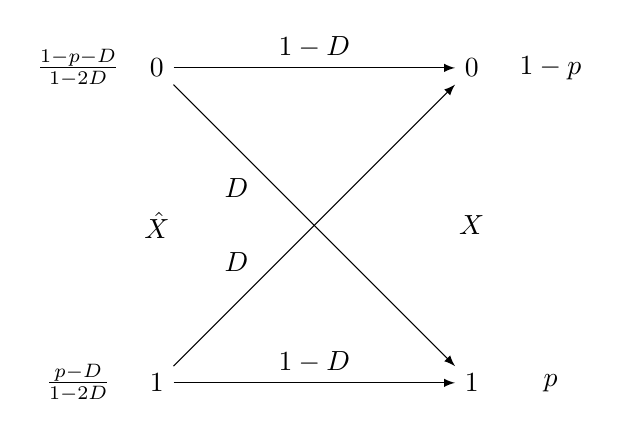
\begin{tikzpicture}[auto]
	\node (s00) at (-1,4) {$\frac{1-p-D}{1-2D}$};
	\node (s0) at (0,4) {$0$};
	\node (s11) at (-1,0) {$\frac{p-D}{1-2D}$};
	\node (s1) at (0,0) {$1$};
	\node (d00) at (5,4) {$1-p$};
	\node (d0) at (4,4) {$0$};
	\node (d11) at (5,0) {$p$};
	\node (d1) at (4,0) {$1$};
	
	\node (xh) at (0,2) {$\hat{X}$};
	\node (x) at (4,2) {$X$};
	
	\draw[-latex] (s0) to node {$1-D$} (d0);
	\draw[-latex] (s0) to node[swap, pos=0.3] {$D$} (d1);
	\draw[-latex] (s1) to node[pos=0.3] {$D$} (d0);
	\draw[-latex] (s1) to node {$1-D$} (d1);
\end{tikzpicture}
\end{figure}





\subsection{The rate distortion theorem}



\paragraph{Definitions}
Assume that we have a source that produces a sequence $X_1,\ldots,X_n$ i.i.d. $\sim p(x)$.\\
~\\
The encoder describes the sequence $X^n$ by an index $f_n(X^n) \in \{1,\ldots,2^{nR}\}$.\\
~\\
The decoder represents $X^n$ by an estimate $\hat{X}^n$.


\begin{figure}
\centering
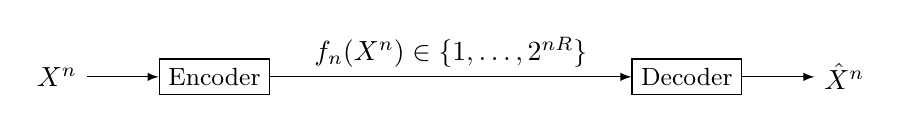
\begin{tikzpicture}[auto]
	\node (s) at (0,0) {$X^n$}; %{\small{Message}};
	\node[draw] (e) at (2,0) {\small{Encoder}};
	\node[draw] (d) at (8,0) {\small{Decoder}};
	\node (r) at (10,0) {$\hat{X}^n$}; %{\small{Estimate}};
	
	\draw[-latex] (s) -- (e);
	\draw[-latex] (e) to node {$f_n(X^n) \in \{1,\ldots, 2^{nR}\}$} (d);
	\draw[-latex] (d) -- (r);
\end{tikzpicture}
\end{figure}





The distortion between $x^n$ and $\hat{x}^n$ is the average
$$
	d(x^n, \hat{x}^n) = \frac{1}{n} \sum_{i=1}^n d(x_i, \hat{x}_i).
$$
%(Some consider the maximum instead, but the theory is even harder)\\
~\\
A $(2^{nR},n)$ \Define{rate distortion code} consists of
\begin{enumerate}
	\item An encoding function $f_n : \alphabet{X}^n \to \{1,\ldots,2^{nR}\}$
	
	\item A decoding (a.k.a. reproduction) function $g_n : \{1,\ldots,2^{nR}\} \to \hat{\alphabet{X}}^n $.
\end{enumerate}
The \Define{distortion} of the code is
$$
	\expectation \left( d(X^n, g_n(f_n(X^n))) \right).
$$
The set of $n$-tuples $\hat{X}^n(1) = g_n(1), \ldots, \hat{X}^n(2^{nR}) = g_n(2^{nR})$  constitute the \Important{codebook}, and $f_n^{-1}(1), \ldots, f_n^{-1}(2^{nR})$ are the \Important{assignment regions}.




\paragraph{The rate distortion theorem}
A rate distortion pair $(R,D)$ is \Define{achievable} if there exists a sequence of $(2^{nR},n)$ rate distortion codes $(f_n,g_n)$ such that
$$
	\lim_{n \to \infty} \expectation \left( d( X^n, g_n(f_n(X^n))) \right) \le D.
$$

\begin{theorem}[Rate distortion theorem]
The rate distortion function $R(D)$ is the infimum of rates $R$ such that $(R,D)$ is achievable.
\end{theorem}


\subsection{Exercises}


\begin{exercise}
Consider a source $X$ uniformly distributed in the set $\{1,2,\dots,m\}$. Find the rate distortion function for this source with Hamming distortion.
\end{exercise}





\begin{exercise}[Rate distortion function with infinite distortion]
Find the rate distortion function for $X \sim \text{Bernoulli}(1/2)$ and distortion
\[
	d(x, \hat{x}) = \begin{cases}
	0 &\text{if } x = \hat{x},\\
	1 &\text{if } x=1, \hat{x} = 0,\\
	\infty &\text{if } x=0, \hat{x} = 1.
	\end{cases}
\]
\end{exercise}












\section{Capacity and rate distortion I: The Blahut-Inamoto algorithms}
\label{sec:37}


\section{Capacity and rate distortion II: Gaussian variables}
\label{sec:38}



\subsection{Continuous random variables}


\paragraph{Continuous random variables}
A \Structure{continuous random variable} $X$ is a mapping $p$ from $\mathbb{R}$ to $\mathbb{R}^+$ such that
\[
	 \int_{-\infty}^\infty p(x) dx = 1.
\]


Any element $x \in \alphabet{X}$ is called an event; $p(x)$ is called the probability density function of $X$. We also use the interpretation
\[
	\mathrm{Pr} \{ X \le x\} = \int_{-\infty}^x p(t) dt.
\]

Again, we can create functions of the random variable $X$. We denote the support of $X$ as
\[
	S := \{x \in \mathbb{R} : p(x) > 0\}.
\]


\paragraph{Expectation and standard deviation}
The \Define{expectation} of a continuous random variable $X$ is
\[
	\mathrm{E} X := \int_S x p(x) dx.
\]

The \Structure{variance} of $X$ is
\begin{align*}
	\mathrm{Var} X 	&:= \mathrm{E} (X - \mathrm{E}X)^2\\
					&= \mathrm{E} X^2 - (\mathrm{E} X)^2.
\end{align*}

The \Define{standard deviation} of $X$ is
\[
	\sigma =\sqrt{\mathrm{Var} X}.
\]


\paragraph{Simple examples}
The \Define{uniform distribution} over an interval $[a,b]$ ($b > a$) is defined as
\[
	p(x) = \begin{cases}
		\frac{1}{b-a} &\text{if } a \le x \le b\\
		0 &\text{otherwise}.
	\end{cases}
\]
(Give expectation and variance.)

The most important continuous random variable is the \Define{normal (or Gaussian) distribution} $\alphabet{N}(\mu, \sigma^2)$, defined as
\[
	p(x) = \frac{1}{\sqrt{2 \pi \sigma^2}} \exp^{- \frac{(x-\mu)^2}{2 \sigma^2}}.
\]
It can be proved that
\begin{align*}
	\mathrm{E} \alphabet{N}(\mu, \sigma^2) &= \mu,\\
	\mathrm{Var} \alphabet{N}(\mu, \sigma^2) &= \sigma^2.
\end{align*}




\subsection{Differential entropy}

\paragraph{Differential entropy}

The \Define{differential entropy} $h(X)$ of a continuous random variable $X$ with density $f(x)$ is defined as
\[
	h(X) = - \int_S f(x) \log f(x) dx,
\]
where $S$ is the support of the random variable.\\
~\\
Remarks:
\begin{enumerate}
	\item $h(X)$ does not always exist.
	
	\item Also, $h(X)$ could be negative!
\end{enumerate}




\paragraph{Differential entropy of a uniform distribution}
\begin{example}
Let $X$ have density
\[
	f(x) = \begin{cases}
	1/a & \mbox{if } x \in [0,a]\\
	0 & \mbox{otherwise}.
	\end{cases}
\]
Then
\[
	h(X) = \log a.
\]
\end{example}

This example shows that the differential entropy does take values into account!



\paragraph{Related concepts}
Joint entropy, conditional entropy are defined similarly. So is the \Define{divergence}
$$
	D(f||g) := \int f \log \frac{f}{g}
$$
and the \Define{mutual information}
\begin{align*}
	I(X;Y) &= D(f(x,y) || f(x)f(y))\\
	&= \int f(x,y) \log \frac{f(x,y)}{f(x)f(y)} dx dy.
\end{align*}

We still have $D(f||g) \ge 0$ with equality iff $f=g$ almost everywhere.






\paragraph{A quick note on integration by parts}

You have seen integration by parts on closed intervals $[a,b]$:
$$
	\int_a^b u'(x) v(x) dx =  \left[u(x) v(x) \right]_a^b - \int_a^b u(x) v'(x) dx.
$$

We will have to use integration by parts over (half)-open intervals, such as $(- \infty, \infty)$ or $[0, \infty)$. This is not allowed in general, but we will never meet any bad example, so you can safely assume that integration by parts is always allowed.



\subsection{The Gaussian channel and its capacity}

\paragraph{The Gaussian channel}
This is the most important continuous alphabet channel.

\begin{figure}
\centering
\begin{tikzpicture}
	\node (x) at (0,0) {$X$};
	\node (y) at (4,0) {$Y$};
	\node (z) at (2,2) {$Z$};
	\node[draw, shape=circle] (p) at (2,0) {$+$};
	
	\draw[-latex] (x) -- (p);
	\draw[-latex] (z) -- (p);
	\draw[-latex] (p) -- (y);
\end{tikzpicture}
\end{figure}

The noise $Z$ is drawn from a Gaussian distribution with variance $N$. Thus
\[
	Y = X + Z, \quad Z \sim \alphabet{N}(0,N).
\]

It is also called Additive White Gaussian Noise (\Define{AWGN}) channel.



\paragraph{Capacity: naive approach}
Clearly, if the noise variance is zero, then the receiver receives the transmitted symbol perfectly. Since $X$ can take any real value, the channel can transmit an arbitrary real number with no error.

If the noise variance is non-zero and there is no constraint on the input, we can choose an infinite subset of inputs arbitrarily far apart, so that they are distinguishable at the output with arbitrarily small probability of error. Again, this has infinite capacity.


\paragraph{Power constraint}
Most common limitation on the input is a \Important{power constraint}. We assume an average power constraint: for any codeword $x^n$ transmitted over the channel, we require
$$
	\frac{1}{n} \sum_{i=1}^n x_i^2 \le P.
$$
This channel models many practical situations, such as radio and satellite links. (For wireless channels, we use so-called Rayleigh fading with Gaussian noise.)


The \Define{capacity} of the Gaussian channel with power constraint $P$ is defined as
\[
	C := \max \{I(X;Y) : \expectation(X^2) \le P \}.
\]

\begin{theorem}
The capacity of a Gaussian channel with power constraint $P$ and noise variance $N$ is
$$
	C = \frac{1}{2} \log \left( 1 + \frac{P}{N} \right).
$$
\end{theorem}




% \paragraph{Proof of the theorem}
% We have
% \begin{align*}
% 	I(X;Y) &= h(Y) - h(Y|X)\\
% 	&= h(Y) - h(Z).\\
% \end{align*}

% We have $h(Z) = \frac{1}{2} \log 2 \pi e N$. Also,
% $$
% 	\mathrm{E}Y^2 = P + N,
% $$
% whence
% \begin{align*}
% 	h(Y) &\le \frac{1}{2} \log 2 \pi e (P+N),\\
% 	I(X;Y) &\le \frac{1}{2} \log \left(1 + \frac{P}{N} \right).
% \end{align*}
% The maximum is achieved when $X \sim \alphabet{N}(0,P)$.

% 


%\subsection{Channel coding theorem}

\paragraph{Channel coding theorem for the Gaussian channel}

We will show that the capacity is still the supremum of the achievable rates for the channel: the arguments will be similar to the discrete channel case.

\begin{definition}
$(M,n)$ code for the Gaussian channel with power constraint $P$:
\begin{enumerate}
	\item An index set $\{1,\ldots, M\}$.
	
	\item An encoding function $x^n: \{1,\ldots,M\} \to \alphabet{X}^n$ satisfying the power constraint $P$, i.e. for every codeword
	$$
		\frac{1}{n} \sum_{i=1}^n x_i^2(w) \le P.
	$$
	
	\item A decoding function $g: \alphabet{Y}^n \to \{1,\ldots, M\}$.
\end{enumerate}
\end{definition}

The rate and the probability of error are defined as before.\\
A rate is achievable if the max probability of error tends to zero.




% \paragraph{Achievability}
% \begin{enumerate}
% 	\item \Structure{Codebook generation.} We generate the codewords $X_i(w), i=1,\ldots, n, w = 1, \ldots, M$ i.i.d. $\sim \alphabet{N}(0,P-\epsilon)$.\\
% 	Since $\frac{1}{n} \sum_i X_i^2 \to P-\epsilon$, the probability that a codeword does not satisfy the power constraint is very small.
	
% 	\item \Structure{Encoding.} To transmit the message $w \in \{1,\ldots, M\}$, the sender sends $X^n(w)$.
	
% 	\item \Structure{Decoding.} Joint typical decoding  (and returns error if the chosen codeword does not satisfy the power constraint).
	
% 	\item \Structure{Probability of error.} Without loss, assume that the codeword $1$ was sent: $Y^n = X^n(1) + Z^n$.
% \end{enumerate}
% 

% \paragraph{Probability of error}
% Let
% \begin{align*}
% 	E_0 &= \left\{ \frac{1}{n} \sum_{i=1}^n X_i^2(1) > P \right\},\\
% 	E_w &= \{ (X^n(w), Y^n) \in A_\epsilon^{(n)} \}.
% \end{align*}

% Then for $n$ large enough and $R < I(X;Y) - 3 \epsilon$,
% \begin{align*}
% 	\mathrm{Pr}\{E\} &= \mathrm{Pr}\{E | W=1\}\\
% 	&= \mathrm{Pr}\{E_0 \cup E_1^c \cup E_2 \cup \ldots \cup E_{2^{nR}}\}\\
% 	&\le 3 \epsilon.
% \end{align*}
% (The joint AEP for continuous variables is the same as the one for discrete variables.)\\
% ~\\
% Again, choose a good codebook and delete half the codewords to finish the proof.
% 

% \paragraph{Converse}
% Consider any $(2^{nR},n)$ code that satisfies the power constraint.\\
% ~\\
% The uniform distribution over $\{1,\ldots,2^{nR}\}$ induces a probability distribution on $x^n(w)$ and $y^n$. We use Fano's inequality:
% $$
% 	H(W|Y^n) \le 1 + nRP_e^{(n)} = n\epsilon_n,
% $$
% where $\epsilon_n \to 0$ as $P_e^{(n)} \to 0$. Hence
% \begin{align*}
% 	nR &= H(W)\\
% 	&= I(W; Y^n) + H(W| Y^n)\\
% 	&\le h(Y^n) - h(Z^n) + n \epsilon_n\\
% 	&\le \sum_{i=1}^n (h(Y_i) - h(Z_i)) + n \epsilon_n.
% \end{align*}
% 

% \paragraph
% Now let $P_i$ be the average power of the $i$-th column of the codebook, i.e.
% $$
% 	P_i := \frac{1}{2^{nR}} \sum_w x_i^2(w).
% $$
% Since the average power of $Y_i$ is $P_i + N$, we obtain
% \begin{align*}
% 	h(Y_i) &\le \frac{1}{2} \log 2 \pi e (P_i + N),\\
% 	\frac{1}{n} \sum_{i=1}^n (h(Y_i) - h(Z_i)) &\le \frac{1}{2n} \sum_{i=1}^n \log \left( 1 + \frac{P_i}{N} \right)\\
% 	&\le \frac{1}{2} \log \left( 1 + \frac{P}{N} \right),\\
% 	R &\le \frac{1}{2} \log \left( 1 + \frac{P}{N} \right) + \epsilon_n.
% \end{align*}
% (We have used $\frac{1}{n} \sum_i P_i \le P$ and the concavity of $f(x) = \frac{1}{2} \log(1 + x)$.)
% 


%\paragraph{Exercises}
%
%\begin{enumerate}
	%\item Fill the gaps in upper bound on mutual information
	%
	%\item Fill in the gaps in upper bound on probability of error
%\end{enumerate}
%
%



\subsection{Rate distortion for a Gaussian source}


\paragraph{Gaussian source}

Let us use a Gaussian source with squared error distortion. Therefore, the distortion criterion is
\[
	\expectation(X - \hat{X})^2 \le D.
\]

\begin{theorem} \label{th:gaussian_R}
For an $\alphabet{N}(0,\sigma^2)$ source with squared error distortion,
\[
	R(D) = \begin{cases}
	\frac{1}{2} \log \frac{\sigma^2}{D}, & 0 \le D \le \sigma^2\\
	0, & D > \sigma^2.
	\end{cases}
\]
\end{theorem}



\subsection{Exercises}


Recall that a random variable $X \sim \alphabet{N}(0, \sigma^2)$ under a normal distribution with zero mean and standard deviation $\sigma$ has density
$$
	\phi(x) = \frac{1}{\sqrt{2\pi \sigma^2}} e^{-\frac{x^2}{2 \sigma^2}} \quad x \in \mathbb{R}.
$$

\begin{exercise}
Prove that 
$$
	h(X)  = \frac{1}{2} \log 2 \pi e \sigma^2 \, \text{bits}.
$$
Hint: You may find it easier to compute the entropy in nats:
$$
	h_e(X) = - \int \phi \ln \phi \,\,\text{nats},
$$
and then $h(X) = \frac{1}{\ln 2} h_e(X)$.
\end{exercise}


\begin{remark}
Since $h(Z + a) = h(Z)$ for any random variable $Z$ and any $a \in \mathbb{R}$, any normal distribution $\alphabet{N}(a,\sigma)$ will have the same differential entropy as above.
\end{remark}



\begin{exercise}
Prove that for any $Y$ with standard deviation $\sigma$, $h(Y) \le h(X)$ for $X \sim \alphabet{N}(0,\sigma^2)$. 
\end{exercise}


\begin{exercise}
Consider $k$ parallel Gaussian channels 
\[
	Y_j = X_j + Z_j, \quad j=1, 2, \dots, k
\]
where $Z_j \sim \alphabet{N}(0, N_j)$, and the noise is assumed to be independent from channel to channel. Consider a common power constraint on the total power of the inputs, i.e.
\[
	\expectation \left( \sum_{j=1}^k X_j^2 \right) \le P.
\]
In order to simplify notation, we denote $X = (X_1, \dots, X_k)$ and $Y = (Y_1, \dots, Y_k)$.

Show that 
\[
	I(X; Y) \le \sum_{j=1}^k \frac{1}{2} \log \left( 1 + \frac{ P_j }{ N_j } \right),
\]
where $P_j = E X_j^2$ and $\sum_j P_j = P$. Give an input distribution which reaches that value.
\end{exercise}



\begin{exercise}
\begin{enumerate}
	\item Let $Y_1$ and $Y_2$ be conditionally independent given $X$. Prove that
	\[
		I(X; Y_1, Y_2) = I(X; Y_1) + I(X; Y_2) - I(Y_1; Y_2).
	\]
	
	\item Let $K$ be a Gaussian channel, with input $X$ and output $Y = X + Z$ and $Z \sim \alphabet{N}(0,N)$. Consider the ``two-step'' Gaussian channel $K'$, where the input $X$ is sent through $K$ twice, hence the output is $(Y_1, Y_2) = (X + Z_1, X + Z_2)$ and $Z_1, Z_2$ are i.i.d. $ \sim \alphabet{N}(0,N)$. Based on the previous item, show that the capacity of the ``two-step'' Gaussian channel is no more than twice than the capacity of the original Gaussian channel.
\end{enumerate}
\end{exercise}



\begin{exercise}
Prove Theorem \ref{th:gaussian_R}. Hint: the proof is similar to the Hamming rate distortion function of a Bernoulli variable. For instance, for the second part of the proof yuo want to consider this channel:

\begin{center}
\begin{tikzpicture}
	\node (x) at (0,0) {$\hat{X} \sim \alphabet{N}(0,\sigma^2 - D)$};
	\node (y) at (6,0) {$X \sim \alphabet{N}(0,\sigma^2)$};
	\node (z) at (3,2) {$Z \sim \alphabet{N}(0, D)$};
	\node[draw, shape=circle] (p) at (3,0) {$+$};
	
	\draw[-latex] (x) -- (p);
	\draw[-latex] (z) -- (p);
	\draw[-latex] (p) -- (y);
\end{tikzpicture}
\end{center}

\end{exercise}














\section{Secrecy I: Cryptosystems}
\label{sec:39}


\subsection{Cryptosystems and perfect secrecy}

\paragraph{Definition}
A \Structure{cryptosystem} is a five-tuple $(\alphabet{P}, \alphabet{C}, \alphabet{K}, \alphabet{E}, \alphabet{D} )$, where
\begin{enumerate}
	\item $\alphabet{P}$ is a finite set of possible plaintexts $x$.
	
	\item $\alphabet{C}$ is a finite set of possible ciphertexts $y$.
	
	\item $\alphabet{K}$, the keyspace, is a finite set of possible keys $k$.
	
	\item $\alphabet{E}$ is a set of encryption rules $e_k : \alphabet{P} \to \alphabet{C}$ for every $k \in \alphabet{K}$.
	
	\item $\alphabet{D}$ is a set of decryption rules $d_k : \alphabet{C} \to \alphabet{P}$ for every $k \in \alphabet{K}$.
	
	\item For each $k \in \alphabet{K}$, we have
	\[
		d_k( e_k(x) ) = x 
	\]
	for every plaintext $x \in \alphabet{P}$.
\end{enumerate}

Note: since $e_k$ is injective, we have $|\alphabet{C}| \ge |\alphabet{P}|$. Also, we have $|\alphabet{E}| = |\alphabet{D}| = |\alphabet{K}|$.





(Give the figure.)




% \paragraph{Shift cipher}

% For the \Define{shift cipher}, $\alphabet{P} = \alphabet{C} = \alphabet{K} = \mathbb{Z}_q$, where
% \begin{align*}
% 	e_k(x) &= (x + k) \mod q,\\
% 	d_k(x) &= (x - k) \mod q.
% \end{align*}

% Then for any $x \in \mathbb{Z}_q$,
% \[
% 	d_k(e_k(x)) = x.
% \]

% We can use it for $q = 26$ and $A \cong 0$, $B \cong 1$, $\dots$, $Z \cong 25$.





\paragraph{Perfect secrecy}
Assumptions:
\begin{enumerate}
	\item The key is chosen (by Alice and Bob) using some fixed probability distribution $K$.

	\item The plaintext is chosen at random according to a random variable $P$.
	
	\item Since the key is chosen before Alice knows what the plaintext will be, $K$ and $P$ are independent random variables.
	
	\item The ciphertext is also a random variable $C$.
\end{enumerate}

%Denote $C(K) = \{ e_K(x) : x \in \alphabet{P} \}$.





\paragraph{Perfect secrecy}

We say that a cryptosystem has \Define{perfect secrecy} if one of the following equivalent properties is satisfied.
\begin{enumerate}
	\item $p(x | y) = p(x)$ for all $x \in \alphabet{P}$, $y \in \alphabet{C}$.
	
	\item $P$ and $C$ are independent.
	
	\item $I(P;C) = 0$.
\end{enumerate}

In other words, the ciphertext gives nothing away about the plaintext.




\paragraph{The shift cipher has perfect secrecy}
\begin{theorem}
Suppose the shift cipher is used, where each key is used with equal probability (i.e. $K$ is uniform). Then for any plaintext probability $P$, the shift cipher has perfect secrecy.
\end{theorem}

\begin{proof}
We have
\[
	I(P;C) = H(C) - H(C | P) = H(C) - H(K) \le 0.
\]
Thus $I(P;C) = 0$ and we have perfect secrecy.
\end{proof}

As an aside, we have also proved that $H(C) = H(K) = \log q$ in that case: the ciphertexts are also equiprobable.



\subsection{Spurious keys and unicity distance}


\paragraph{Key equivocation}
The conditional entropy $H(K | C)$ is called the \Define{key equivocation:} that's how much uncertainty is left about the key when the ciphertext is known.

\begin{theorem} 
For any cryptosystem, the key equivocation is given by
\[
	H(K|C) = H(K) + H(P) - H(C).
\]
\end{theorem}

\begin{proof} 
We have
\[
	H(K,P,C) = H(C | P,K) + H(K,P) = H(K) + H(P),
\]
since the encoding is deterministic ($H(C | K,P) = 0$) and the key and the plaintext are independent ($I(K;P) = 0$).

Similarly, we also have
\[
	H(K,P,C) = H(P | C, K) + H(K, C) = H(C) + H(K | C).
\]
Combining, we obtain the result.
\end{proof}


\paragraph{Spurious keys}
Suppose a string of plaintext $x^n = x_1 x_2 \dots x_n$ is encrypted using one key, producing $y^n = y_1 y_2 \dots y_n$.

Eve wants to determine the key. We are looking at ciphertext-only attacks, and we assume that Eve has infinite computational power. We also assume that Eve knows the plaintext is in a ``natural'' language, such as English. In general, Eve will be able to rule out certain keys, but many ``possible'' keys remain, only one of which is the correct key. The remaining possible, but incorrect, keys are the spurious keys.

For example, say the shift cipher is used and Eve receives \texttt{WNAJW}, then we can check that there are only two meaningful plaintexts, namely \texttt{RIVER} and \texttt{ARENA}, for encryption keys \texttt{F} and \texttt{W}. One of these is correct, the other one is spurious.




\paragraph{Language redundancy}
Let $P^n$ be the random distribution on all $n$-grams of plaintext. The entropy (per letter) of a natural language $L$ is
\[
	H_L = \lim_{n \to \infty} \frac{ H(P^n) }{ n }.
\]
For instance, for the English language, we have (roughly)
\[
	H(P) \sim 4.19, \quad H(P^2) \sim 3.90, \quad  \dots \quad H_L \le 1.5.
\]
The \Define{redundancy} of the language $L$ is defined as
\[
	R_L = 1 - \frac{ H_L }{ \log |\alphabet{P}| }.
\]




\paragraph{Bound on the number of spurious keys}
\begin{theorem}
Consider a cryptosystem with $|\alphabet{C}| = |\alphabet{P}|$ and uniform key. Then given a string of ciphertext of length $n$ ($n$ large enough), the expected number of spurious keys $s_n$ satisfies
\[
	s_n \ge \frac{ |\alphabet{K}| }{ |\alphabet{P}|^{n R_L} } - 1.
\]
\end{theorem}

Note: the RHS tends to zero exponentially quickly as $n \to \infty$.
 

\begin{proof}
The key equivocation is
\[
	H(K | C^n) = H(K) + H(P^n) - H(C^n),
\]
where 
\begin{align*}
	H(K) 	&= 		\log |\alphabet{K}|,\\
	H(P^n) 	&\sim 	n H_L = n (1 - R_L) \log |\alphabet{P}|,\\
	H(C^n) 	&\le 	n \log |\alphabet{C}| = n \log |\alphabet{P}|.
\end{align*}
Thus,
\[
	H(K | C^n) \ge \log |\alphabet{K}| - n R_L \log |\alphabet{P}|.
\]

Given $y^n \in \alphabet{C}^n$, let 
\[
	K(y^n) = \{ K \in \alphabet{K} : \exists x^n \in \alphabet{P}^n, p(x^n) > 0, e_K(x^n) = y^n \},
\]
then $s_n + 1 = \sum_{y^n} p(y^n) |K(y^n)|$.

We can relate it to the key evocation as follows.
\begin{align*}
	H(K | C^n) &= \sum_{y^n \in \alphabet{C}^n} p(y^n) H(K | y^n)\\
	&\le \sum_{y^n \in \alphabet{C}^n} p(y^n) \log |K(y^n)|\\
	&\le \log \sum_{y^n \in \alphabet{C}^n} p(y^n) |K(y^n)|\\
	&= \log (s_n + 1).
\end{align*}
Combining, we obtain the result.

\end{proof}

\paragraph{Unicity distance}
The \Define{unicity distance} of a cryptosystem is defined to be the value of $n$ at which the expected number of spurious keys becomes zero. In other words, it is the average amount of ciphertext required for an opponent to be able to uniquely compute the key (given enough computing time).

We have
\[
	s_n \ge \frac{ |\alphabet{K}| }{ |\alphabet{P}|^{n R_L} } - 1.
\]
If we view the RHS as an actual estimate for $s_n$ and solve for $n$, we get that the unicity distance is about
\[
	\frac{ \log |\alphabet{K}| }{ R_L \log |\alphabet{P}| }.
\]
Some people then use this estimate as their \textit{de facto} definition.




\subsection{Exercises}




\begin{exercise}
let $n$ be a positive integer. A Latin square of order $n$ is an $n \times n$ array $L$ of the integers $[n] = \{1, \dots, n\}$ such that every one of the $n$ integers occurs exactly once in every row and every column of $L$. An example of a Latin square of order $4$ is given as follows.
\[
	L = \begin{pmatrix}
	1 & 2 & 3 & 4\\
	2 & 3 & 4 & 1\\
	3 & 4 & 1 & 2\\
	4 & 1 & 2 & 3
	\end{pmatrix}.
\]

\begin{enumerate}
	\item For any $n$, give a construction of a Latin square of order $n$. (Actually, there are incredibly many of those!)
	
	\item Given a Latin square $L$ of order $n$, define a cryptosystem with $\alphabet{K} = \alphabet{P} = \alphabet{C} = [n]$ which has perfect secrecy if $\alphabet{K}$ is uniform. 
\end{enumerate}
\end{exercise}




\begin{exercise}
Suppose a cryptosystem achieves perfect secrecy for a particular plaintext probability distribution. Prove that perfect secrecy is maintained for any plaintext distribution.
\end{exercise}





\begin{exercise}
Prove that if a cryptosystem has perfect secrecy and $|\alphabet{K}| = |\alphabet{C}| = |\alphabet{P}|$, then every cipherext is equiprobable.
\end{exercise}









\section{Secrecy II: Secrecy capacity}
\label{sec:40}



%\title{Secrecy II\\Secrecy capacity}


\subsection{Perfect secrecy}

\paragraph{Perfect secrecy revisited}
(Use same notation as previous lecture)

A sender (Alice) wishes to communicate a message $M \in [2^{nR}]$ to a receiver
(Bob) over a public channel in the presence of an eavesdropper (Eve) who
observes the channel output. Alice and Bob share a key $K \in \mathbb{N}$, which is
unknown to Eve. 

How many key bits $(H(K))$ are needed so that Eve cannot obtain any information about the message?

\begin{center}
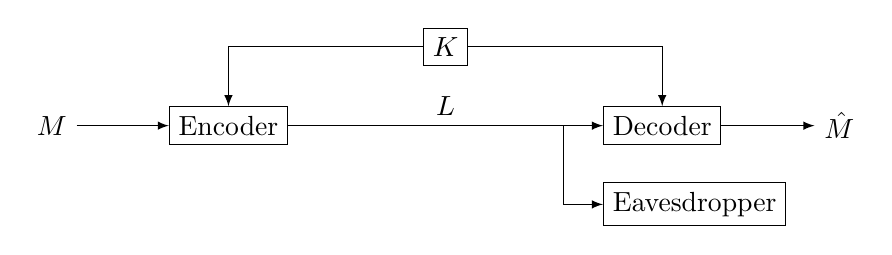
\begin{tikzpicture}
	%\draw (0,0) rectangle (4,4);
	
	\node 						(M)		at (0,1)	{$M$};
	\node[draw, left] 			(Enc)	at (3,1) 	{Encoder};
	\node[draw] 				(K) 	at (5,2) 	{$K$};
	\node[draw, right] 			(Dec)	at (7,1) 	{Decoder};
	\node 						(HM)	at (10,1) 	{$\hat{M}$};
	\node[draw, right] 			(Eve)	at (7,0) 	{Eavesdropper};
	
	\draw[-latex] (M) 	-- (Enc);
	\draw[-latex] (Enc) -- (Dec) node[pos=0.5, above]{$L$};
	\draw[-latex] (Dec)	-- (HM);
	
	\draw[-latex] (K) -| (Enc);
	\draw[-latex] (K) -| (Dec);	
	\draw[-latex] (6.5,1) |- (Eve);
\end{tikzpicture}
\end{center}



\paragraph{Perfect secrecy}

The message (plaintext) is uniform: $M \sim U(2^{nR})$. The encoder (encryption function) assigns a ciphertext $c(m,k)$ to each message $m \in [2^{nR}]$ and key $k$, and the decoder (decryption function) assigns a message $\hat{m}(c,k)$ to each ciphertext $c$ and key $k$. The communication system is said to have \Define{perfect secrecy} if
\begin{itemize}
	\item $\probability( M \ne \hat{M}( C(M,K), K ) ) = 0$, i.e. the message is decoded correctly, and
	
	\item the information leakage $I(C;M) = 0$, i.e. the ciphertext reveals no information about the message.
\end{itemize}



\paragraph{Perfect secrecy theorem}

\begin{theorem}[Shannon's perfect secrecy theorem]
The system has perfect secrecy if and only if $H(K) \ge H(M)$. (Check the very statement.)
\end{theorem}

\begin{proof}
For perfect secrecy, we must have
\begin{align*}
	H(M) &= H(M | C)\\
	&\le H(M, K | C)\\
	&= H(K | C)\\
	&\le H(K).
\end{align*} 
To prove sufficiency, use the shift cipher for instance.
\end{proof}


\paragraph{Consequences of perfect secrecy}
So this is bad news! Alice and Bob need to share a key as long as the message
itself. There are several directions to avoid this limitation of Shannon's secrecy system
\begin{itemize}
    \item Computational security: how to exploit the computational hardness of
    recovering the message from the ciphertext without knowing the key?
    
    \item \Important{Wiretap channel:} how to use the better quality of Alice-Bob channel to outdo
    Eve
\end{itemize}
We shall take a look at the wiretap channel.




\subsection{Secrecy capacity}



\paragraph{Secure Communication over a DMC}
Consider the following extension of the Shannon secrecy system to DMC.\\
~\\
\begin{center}
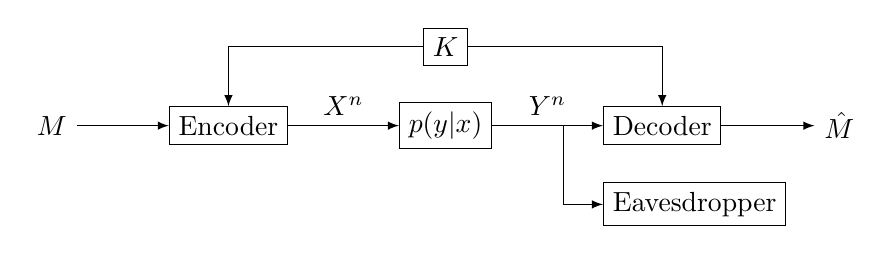
\begin{tikzpicture}
	%\draw (0,0) rectangle (4,4);
	
	\node 						(M)		at (0,1)	{$M$};
	\node[draw, left] 			(Enc)	at (3,1) 	{Encoder};
	\node[draw] 				(K) 	at (5,2) 	{$K$};
	\node[draw, right] 			(Dec)	at (7,1) 	{Decoder};
	\node 						(HM)	at (10,1) 	{$\hat{M}$};
	\node[draw, right] 			(Eve)	at (7,0) 	{Eavesdropper};
	\node[draw]					(C)		at (5,1) 	{$p(y|x)$};
	
	\draw[-latex] (M) 	-- (Enc);
	\draw[-latex] (Enc) -- (C) node[pos=0.5, above]{$X^n$};
	\draw[-latex] (C)	-- (Dec) node[pos=0.5, above]{$Y^n$};
	\draw[-latex] (Dec)	-- (HM);
	
	\draw[-latex] (K) -| (Enc);
	\draw[-latex] (K) -| (Dec);	
	\draw[-latex] (6.5,1) |- (Eve);
\end{tikzpicture}
\end{center}


\paragraph{Secrecy codes}
Formally, a $(2^{nR}, 2^{n R_K}, n)$ secrecy code for the Shannon system consists of:
\begin{enumerate}
	\item A message set $[2^{nR}]$ and a key set $[2^{nR_K}]$

	\item A randomized encoder that generates codeword $X^n(m, k) \in \alphabet{X}^n$ according to the conditional pmf $p(x^n|m, k)$ for each message-key pair
	$(m, k) \in [2^{nR}] \times [2^{nR_K}]$
	
	\item A decoder that assigns a message $\hat{m}(y^n, k)$ or an error message $e$ to each
	received sequence $y^n \in \alphabet{Y}^n$ and key $k \in [2^{nR_K}]$
\end{enumerate}



\paragraph{Information leakage}

We assume that the message-key pair $(M,K)$ is uniformly distributed over
$[2^{nR}] \times [2^{nR_K}]$. The \Define{information leakage rate} associated with the $(2^{nR}, 2^{nR_K}, n)$ secrecy code is defined as
\[
	R_l^{(n)} = \frac{1}{n} I(M; Y^n).
\]
The average probability of error for the secrecy code is defined as
\[
	P_e^{(n)} = \probability( M \ne \hat{M}(Y^n, K) ).
\]
A rate $R$ is \Define{achievable} at key rate $R_K$ if there exists a sequence of
$(2^{nR}, 2^{nR_K}, n)$ codes with $R_l^{(n)} \to 0$ and $P_e^{(n)} \to 0$ as $n \to \infty$


\paragraph{Secrecy capacity}
The \Define{secrecy capacity} $C(R_K)$ of the DMC as the supremum of all achievable
rates at key rate $R_K$.

This asymptotic notion of secrecy is weaker than Shannon's original notion of
perfect secrecy. Can we send at a higher rate?

\begin{theorem} 
The secrecy capacity is
\[
	C(R_K) = \min \left\{ R_K, \; \max_{p(x)}\, I(X;Y) \right\}.
\]
\end{theorem}
Thus secure communication is still limited by the key rate until saturated by the
channel capacity.



\subsection{The wiretap channel}



\paragraph{The Wiretap Channel}
A discrete-memoryless wiretap channel (\Define{DM-WTC}) $(\alphabet{X}, p(y, z|x), \alphabet{Y} \times \alphabet{Z})$ is a DM-Broadcast Channel with sender $X$, legitimate receiver $Y$ and eavesdropper $Z$.

The sender $X$ wishes to send a message $M \in [2^{nR}]$ reliably to the receiver
$Y$ while keeping it secret from the eavesdropper $Z$.

\begin{center}
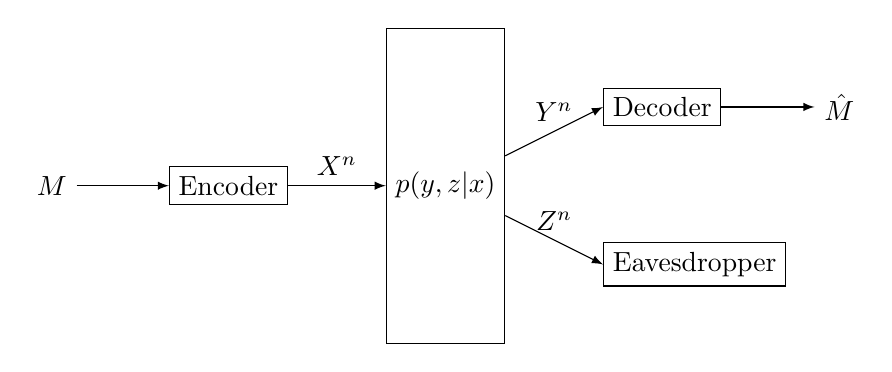
\begin{tikzpicture}
	%\draw (0,0) rectangle (4,4);
	
	\node 							(M)		at (0,2)	{$M$};
	\node[draw, left] 				(Enc)	at (3,2) 	{Encoder};
	\node[draw, right] 				(Dec)	at (7,3) 	{Decoder};
	\node 							(HM)	at (10,3) 	{$\hat{M}$};
	\node[draw, right] 				(Eve)	at (7,1) 	{Eavesdropper};
	\node[draw, minimum height=4cm]	(C)		at (5,2) 	{$p(y,z|x)$};
	
	\draw[-latex] (M) 	-- (Enc);
	\draw[-latex] (Enc) -- (C) node[pos=0.5, above]{$X^n$};
	\draw[-latex] (C)	-- (Dec.west) node[pos=0.5, above]{$Y^n$};
	\draw[-latex] (Dec)	-- (HM);
	\draw[-latex] (C)	-- (Eve.west) node[pos=0.5, above]{$Z^n$};

\end{tikzpicture}
\end{center}



\paragraph{Codes for the wiretap channel}

A $(2^{nR}, n)$ \Define{secrecy code} for the DM-WTC consists of:
\begin{enumerate}
	\item A message set $[2^{nR}]$

	\item A randomized encoder that generates a codeword $X^n(m)$, $m \in [2^{nR}]$,
according to $p(x^n|m)$

	\item A decoder that assigns a message $\hat{m}(y^n)$ or an error message $e$ to each
received sequence $y^n \in \alphabet{Y}^n$
\end{enumerate}

The message is drawn uniformly at random: $M \sim U[2^{nR}]$. The \Define{information leakage rate} is defined as 
\[
	R_l^{(n)} := \frac{1}{n} I(M;Z^n)
\]


\paragraph{Secrecy capacity of the wiretap channel}
The probability of error, achievability, and the secrecy capacity $C_S$ are defined as
for the problem of secure communication over DMC.

\begin{theorem} 
The secrecy capacity of the DM-WTC $(\alphabet{X}, p(y, z|x), \alphabet{Y} \times \alphabet{Z})$ is given by
\[
	C_S = \max_{p(u,x)} ( I(U; Y ) - I(U;Z) )
\]
for $|\alphabet{U}| \le |\alphabet{X}|$.
\end{theorem}


\paragraph{Physically degraded wiretap channel}


The wiretap channel was first introduced by Wyner, who assumed that the
channel to the eavesdropper is a physically degraded version of the channel to
the receiver, i.e. $p(y, z|x) = p(y|x)p(z|y)$. Under this assumption,
\begin{align*}
I(U; Y ) - I(U;Z) 	&= I(U; Y |Z)\\
					&\le I(X; Y |Z)\\
					&= I(X; Y ) - I(X;Z)
\end{align*}
Hence, the secrecy capacity in this case is
\[
	C_S = \max_{p(x)} (I(X; Y ) - I(X;Z)).
\]




\paragraph{Binary Symmetric Wiretap Channel}

Consider the BS-WTC: 
\begin{align*}
	Y &= X \oplus Z_1,\\
	Z &= X \oplus Z_2,
\end{align*}
where $Z_1$ and $Z_2$ are independent $Bern(p_1)$ and $Bern(p_2)$ variables, respectively.

\begin{theorem} 
The secrecy capacity for this channel is
\[
	C_S = \begin{cases}
		H(p_2) - H(p_1) &\text{for } p_2 \ge p_1,\\
		0 &\text{otherwise}.
	\end{cases}
\]
\end{theorem}


\subsection{Exercises}


\begin{exercise}
Prove that the secrecy capacity for the BS-WTC channel is
\[
	C_S = \begin{cases}
		H(p_2) - H(p_1) &\text{for } p_2 \ge p_1,\\
		0 &\text{otherwise}.
	\end{cases}
\]
\end{exercise}















\bibliographystyle{plain}
\bibliography{codes_and_cryptography}





\end{document}
